\documentclass[a4paper]{report}

% ===================================================
% 1. CẤU HÌNH CƠ BẢN VÀ TIẾNG VIỆT
% ===================================================
\usepackage[utf8]{inputenc}
\usepackage{vntex} % Hỗ trợ tiếng Việt chuẩn
\usepackage[a4paper, left=2cm, right=2cm, top=2cm, bottom=3.5cm]{geometry}
\usepackage{indentfirst} % Thụt đầu dòng đoạn văn đầu tiên
\usepackage{setspace} % Cãn giãn dòng
\usepackage{parskip} % Xử lý khoảng cách giữa các đoạn

% ===================================================
% 2. TOÁN HỌC VÀ KHOA HỌC
% ===================================================
\usepackage{amsmath, amssymb, latexsym, mathtools}
\usepackage[overload]{empheq}
\usepackage[thinc]{esdiff} % Viết đạo hàm đẹp
\usepackage{systeme} % Hệ phương trình

% ===================================================
% 3. HÌNH ẢNH VÀ ĐỒ HỌA
% ===================================================
\usepackage{graphicx} % Chuẩn mới thay cho graphics/epsfig
\usepackage{subcaption} % Hình phụ (a, b)
\usepackage{float} % Để dùng [H] cho hình ảnh đứng yên
\usepackage{placeins} % Lệnh \FloatBarrier
\usepackage{tikz} % Vẽ hình vector
\usetikzlibrary{arrows,snakes,backgrounds,calc}

% ===================================================
% 4. BẢNG BIỂU (TABLES)
% ===================================================
\usepackage{array, tabularx, caption}
\usepackage{ltablex, multirow, multicol}
\usepackage{hhline}
\usepackage{colortbl} % Tô màu bảng
\usepackage{longtable}

% ===================================================
% 5. ĐỊNH DẠNG VÀ KHUNG (FORMATTING & FRAMES)
% ===================================================
\usepackage[table]{xcolor} % Gom xcolor vào 1 chỗ
\usepackage{titlesec} % Định dạng tiêu đề chương/mục
\usepackage{mdframed} % Khung văn bản
\usepackage{tcolorbox} % Hộp màu đẹp hơn
\usepackage{longfbox}
\usepackage{fancyhdr} % Header và Footer
\usepackage{enumitem} % Thay thế cho enumerate, mạnh mẽ hơn

% ===================================================
% 6. CODE VÀ THUẬT TOÁN
% ===================================================
\usepackage[lined,boxed,commentsnumbered]{algorithm2e}
\usepackage{listings}
\usepackage{courier} % Font chữ cho code

\usepackage{amsmath, amssymb, amsfonts} % Toán học
\usepackage{graphicx}
\usepackage{hyperref}
\usepackage{indentfirst}
\usepackage{float}     % Để cố định vị trí hình ảnh/bảng [H]
\usepackage{booktabs}  % Kẻ bảng đẹp (\toprule, \midrule)
\usepackage{xcolor}
\usepackage{array}     % Căn chỉnh bảng tốt hơn
\usepackage{longtable} % Bảng dài qua trang
\usepackage{listings}  % Hiển thị code/SQL

\usepackage{xurl}

% --- CẤU HÌNH CODE LISTING ---
\lstset{
  basicstyle=\ttfamily\small,
  breaklines=true,
  frame=single,
  backgroundcolor=\color{gray!10},
  keywordstyle=\color{blue}\bfseries,
  commentstyle=\color{green!50!black},
  stringstyle=\color{red},
  showstringspaces=false
}

% --- CẤU HÌNH VẼ HÌNH (TIKZ) ---
\usepackage{tikz}
\usetikzlibrary{shapes.geometric, arrows, positioning, fit, backgrounds, calc, shadows}

% --- ĐỊNH DẠNG ---
\setlength{\parskip}{6pt}
\renewcommand{\baselinestretch}{1.2}

% --- FLOAT SPACING (giảm khoảng trắng quanh ảnh) ---
\setlength{\textfloatsep}{10pt plus 2pt minus 4pt}
\setlength{\floatsep}{8pt plus 2pt minus 4pt}
\setlength{\intextsep}{8pt plus 2pt minus 4pt}
\setlength{\dbltextfloatsep}{10pt plus 2pt minus 4pt}
\renewcommand{\topfraction}{0.85}
\renewcommand{\bottomfraction}{0.70}
\renewcommand{\textfraction}{0.10}
\renewcommand{\floatpagefraction}{0.80}

% --- LỆNH TIỆN ÍCH: link nhảy đến hình ---
% Dùng: \figref{fig:label} -> "Hình X.Y" có thể click
\newcommand{\figref}[1]{\hyperref[#1]{Hình~\ref*{#1}}}

% Định nghĩa màu cho code
\definecolor{dkgreen}{rgb}{0,0.6,0}
\definecolor{gray}{rgb}{0.5,0.5,0.5}
\definecolor{mauve}{rgb}{0.58,0,0.82}

% Cấu hình listings
\lstset{
  frame=tb,
  language=R, % Mặc định là R, có thể đổi khi dùng
  aboveskip=3mm,
  belowskip=3mm,
  showstringspaces=false,
  columns=flexible,
  basicstyle={\small\ttfamily},
  numbers=none,
  numberstyle=\tiny\color{gray},
  keywordstyle=\color{blue},
  commentstyle=\color{dkgreen},
  stringstyle=\color{mauve},
  breaklines=true,
  breakatwhitespace=true,
  tabsize=3
}
\usepackage{tikz}
\usetikzlibrary{shapes, arrows.meta, shapes.geometric, positioning, fit, backgrounds, shadows, matrix}
% ===================================================
% 7. TẠO MỤC LỤC VÀ LIÊN KẾT (LOAD CUỐI CÙNG)
% ===================================================
\usepackage{tocloft} % Định dạng mục lục
\usepackage{lastpage} % Đếm tổng số trang
\usepackage{hyperref} % Tạo link (thường load cuối cùng để tránh lỗi)
\usepackage{fancyvrb}
% Cấu hình Hyperref
\hypersetup{
    urlcolor=black,
    linkcolor=black,
    citecolor=black,
    colorlinks=true
}
% Cấu hình tiêu đề chương (Chapter)
\titlespacing*{\chapter}{0pt}{0pt}{40pt}
\titleformat{\chapter}[hang]
  {\normalfont\Large\bfseries}
  {Chương \thechapter:}
  {1em}
  {}

\setcounter{secnumdepth}{4}
\setcounter{tocdepth}{2}

% Cấu hình Paragraph
\titleformat{\paragraph}
{\normalfont\normalsize\bfseries}{\theparagraph}{1em}{}
\titlespacing*{\paragraph}
{0pt}{3.25ex plus 1ex minus .2ex}{1.5ex plus .2ex}

% Cấu hình Mục lục
\renewcommand{\cfttoctitlefont}{\Huge\bfseries}
\renewcommand{\cftaftertoctitle}{}
\renewcommand{\contentsname}{Mục lục}

% ===================================================
% 8. HEADER & FOOTER SETUP
% ===================================================
\setlength{\headheight}{40pt}
\pagestyle{fancy}
\fancyhead{} % clear all header fields
\fancyhead[L]{
 \begin{tabular}{rl}
    \begin{picture}(25,15)(0,0)
    \put(0,-8){
\includegraphics[width=8mm, height=8mm]{figures/common/hcmut.jpg}}
    \end{picture}&
    \begin{tabular}{l}
        \textbf{\bf \ttfamily  TRƯỜNG ĐẠI HỌC BÁCH KHOA - ĐHQG-HCM}\\
        \textbf{\bf \ttfamily  KHOA KHOA HỌC VÀ KỸ THUẬT MÁY TÍNH }
    \end{tabular}
 \end{tabular}
}
\fancyhead[R]{} % Bên phải header để trống
\fancyfoot{} % clear all footer fields
\fancyfoot[L]{\scriptsize \ttfamily ĐỒ ÁN CHUYÊN NGÀNH - CO4029}
\fancyfoot[R]{\scriptsize \ttfamily Trang {\thepage}/\pageref{LastPage}}
\renewcommand{\headrulewidth}{0.3pt}
\renewcommand{\footrulewidth}{0.3pt}

% Áp dụng header/footer cho trang đầu chương (thường trang chapter sẽ trắng trơn, lệnh này ép nó hiện)
\makeatletter
\let\ps@plain\ps@fancy
\makeatother

% ===================================================
% BẮT ĐẦU NỘI DUNG DOCUMENT
% ===================================================
\begin{document}
\hypersetup{pageanchor=false}
\pagenumbering{roman}
\pagestyle{empty}

% --- TRANG BÌA ---
\begin{titlepage}
    \begin{tikzpicture}[remember picture,overlay,inner sep=0,outer sep=0]
         \draw[blue!70!black,line width=4pt] ([xshift=-1.5cm,yshift=-2cm]current page.north east) coordinate (A)--([xshift=2.4cm,yshift=-2cm]current page.north west) coordinate(B)--([xshift=2.4cm,yshift=2cm]current page.south west) coordinate (C)--([xshift=-1.5cm,yshift=2cm]current page.south east) coordinate(D)--cycle;

         \draw ([yshift=0.5cm,xshift=-0.5cm]A)-- ([yshift=0.5cm,xshift=0.5cm]B)--
         ([yshift=-0.5cm,xshift=0.5cm]B) --([yshift=-0.5cm,xshift=-0.5cm]B)--([yshift=0.5cm,xshift=-0.5cm]C)--([yshift=0.5cm,xshift=0.5cm]C)--([yshift=-0.5cm,xshift=0.5cm]C)-- ([yshift=-0.5cm,xshift=-0.5cm]D)--([yshift=0.5cm,xshift=-0.5cm]D)--([yshift=0.5cm,xshift=0.5cm]D)--([yshift=-0.5cm,xshift=0.5cm]A)--([yshift=-0.5cm,xshift=-0.5cm]A)--([yshift=0.5cm,xshift=-0.5cm]A);

         \draw ([yshift=-0.3cm,xshift=0.3cm]A)-- ([yshift=-0.3cm,xshift=-0.3cm]B)--
         ([yshift=0.3cm,xshift=-0.3cm]B) --([yshift=0.3cm,xshift=0.3cm]B)--
         ([yshift=-0.3cm,xshift=0.3cm]C)--([yshift=-0.3cm,xshift=-0.3cm]C)--([yshift=0.3cm,xshift=-0.3cm]C)-- ([yshift=0.3cm,xshift=0.3cm]D)--([yshift=-0.3cm,xshift=0.3cm]D)--([yshift=-0.3cm,xshift=-0.3cm]D)--([yshift=0.3cm,xshift=-0.3cm]A)--([yshift=0.3cm,xshift=0.3cm]A)--([yshift=-0.3cm,xshift=0.3cm]A);
    \end{tikzpicture}

    \begin{center}
     ĐẠI HỌC QUỐC GIA THÀNH PHỐ HỒ CHÍ MINH \\
     TRƯỜNG ĐẠI HỌC BÁCH KHOA \\
     \textbf{KHOA KHOA HỌC VÀ KỸ THUẬT MÁY TÍNH}
    \end{center}

    \vspace{0.5cm}

    \begin{figure}[h!]
    \begin{center}
     
\includegraphics[width=3cm]{figures/common/hcmut.jpg}
    \end{center}
    \end{figure}

    \vspace{0.5cm}

    \begin{center}
    \begin{tabular}{c}
    \textbf{\Large BÁO CÁO ĐỒ ÁN CHUYÊN NGÀNH}\\
    \\
    \hline
    \\
    \textbf{\large{XÂY DỰNG HỆ THỐNG QUẢN LÝ THƯ VIỆN TRỰC TUYẾN}} \\
    \textbf{\large{TÍCH HỢP AI HỖ TRỢ TÌM KIẾM VÀ GỢI Ý SÁCH}}\\
    \vspace{0.5cm}
    \textbf{\huge }\\
    \hline
    \end{tabular}
    \end{center}

    \vspace{1cm}
    \begin{center}
        \textbf{\large ProjectID: HK251-DAGD1-512} \\
        \textbf{\large NHÓM: HAI ANH TRAI QUẢNG TRỊ} \\
    \end{center}
    \vspace{2cm}

    \begin{table}[h]
        \centering
        \begin{tabular}{rrl}
             & Giảng viên hướng dẫn: & TS. Trương Tuấn Anh \\
             &                       & CN. Dương Huỳnh Anh Đức \\
             & Thành viên:           & Võ Quang Thắng - 2213214\\
             &                       & Hồ Sỹ Thắng - 2213188\\
        \end{tabular}
    \end{table}

    \vspace{2cm}
    \begin{center}
    {\footnotesize TPHCM, tháng 5 năm 2026}
    \end{center}
\end{titlepage}

\newpage
\input{tex/frontmatter/01_acknowledgements}
\newpage
\input{tex/frontmatter/02_abstract}
\newpage
% --- PHẦN TIÊU ĐỀ ---
\thispagestyle{empty}

\noindent
\vspace{0.2cm}
\begin{center}
    \textbf{\LARGE PHÂN CÔNG CÔNG VIỆC}
\end{center}
\vspace{1cm}

\begin{center}
\renewcommand{\arraystretch}{1.5}
\begin{longtable}{|c|p{8.1cm}|p{2.8cm}|p{2.4cm}|}
\hline
\textbf{STT} & \textbf{Nội dung công việc / Chương mục} & \textbf{Sinh viên thực hiện} & \textbf{Ghi chú} \\
\hline
\endfirsthead
\multicolumn{4}{c}%
{\tablename\ -- \textit{Tiếp theo từ trang trước}} \\
\hline
\textbf{STT} & \textbf{Nội dung công việc / Chương mục} & \textbf{Sinh viên thực hiện} & \textbf{Ghi chú} \\
\hline
\endhead
\hline \multicolumn{4}{r}{\textit{Tiếp tục ở trang sau}} \\
\endfoot
\hline
\endlastfoot

% 1. Nghiên cứu
1 & \textbf{Nghiên cứu tổng quan và Cơ sở lý thuyết} \newline
- Chương 1: Giới thiệu dự án \newline
- Chương 2: Kiến thức và công nghệ nền tảng \newline
- Chương 3: Công trình liên quan
& Hồ Sỹ Thắng \newline Võ Quang Thắng & Làm chung \\
\hline

% 2. Phân tích
2 & \textbf{Phân tích yêu cầu và hệ thống đề xuất} \newline
- Chương 4: Hệ thống đề xuất \newline
- Phân tích Use Case, Activity Diagram \newline
- Thiết kế cơ sở dữ liệu, ràng buộc nghiệp vụ và luồng xử lý chính
& Hồ Sỹ Thắng \newline Võ Quang Thắng & Làm chung \\
\hline

% 3. Thiết kế kiến trúc
3 & \textbf{Thiết kế kiến trúc hệ thống (Chương 5)} \newline
- Kiến trúc Modular Monolith + Clean Architecture cho Back-end \newline
- Thiết kế AI Service, schema dữ liệu AI và luồng tích hợp với Back-end \newline
- Xác định luồng giao tiếp giữa Front-end, Back-end, AI Service và hạ tầng dữ liệu
& Hồ Sỹ Thắng \newline Võ Quang Thắng & Làm chung \\
\hline

% 4. Back-end
4 & \textbf{Hiện thực Back-end (Spring Boot)} \newline
- Xây dựng REST API, xử lý nghiệp vụ và phân quyền JWT \newline
- Hiện thực các module quản lý sách, bạn đọc, mượn/trả, đặt trước, phí phạt \newline
- Thiết kế service layer, repository, domain event và tích hợp cơ sở dữ liệu \newline
- Hỗ trợ tích hợp các API phục vụ Front-end và AI Service
& Hồ Sỹ Thắng \newline Võ Quang Thắng & Võ Quang Thắng chính; Hồ Sỹ Thắng hỗ trợ \\
\hline

% 5. AI
5 & \textbf{Hiện thực module AI (Python FastAPI)} \newline
- Tìm kiếm ngữ nghĩa (SBERT + pgvector) \newline
- Hệ thống gợi ý lai ghép (content-based, ALS, trending fallback) \newline
- Pipeline xử lý PDF, chunking, embedding và reduce metadata bằng Gemini \newline
- Thiết kế API nội bộ để Back-end gọi sang AI Service \newline
- Thiết kế fallback khi Gemini/AI lỗi, callback bảo mật bằng HMAC và luồng xử lý nền cho tài liệu PDF
& \textbf{Hồ Sỹ Thắng} & Phụ trách chính \\
\hline

% 6. Front-end
6 & \textbf{Hiện thực Front-end (React + Vite)} \newline
- Thiết kế và hoàn thiện giao diện người dùng cho độc giả, thủ thư và admin \newline
- Tích hợp API Back-end, luồng xác thực, thông báo realtime và các trạng thái nghiệp vụ \newline
- Tích hợp các tính năng AI như tìm kiếm ngữ nghĩa, gợi ý sách và hiển thị metadata
& Hồ Sỹ Thắng \newline Võ Quang Thắng & Làm chung \\
\hline

% 7. Kiểm thử
7 & \textbf{Kiểm thử hệ thống (Chương 7)} \newline
- Kiểm thử Backend: JUnit~5, Mockito, MockMvc, Testcontainers \newline
- Kiểm thử Frontend: Jest, Testing Library, service contract \newline
- Kiểm thử API và các luồng nghiệp vụ chính của hệ thống \newline
- Tổng hợp kết quả test, chụp artifact và đưa bằng chứng kiểm thử vào báo cáo
& Hồ Sỹ Thắng \newline Võ Quang Thắng & Frontend, AI: Hồ Sỹ Thắng; Backend: Võ Quang Thắng; Tích hợp: Làm chung \\
\hline

% 8. Kiểm thử AI
8 & \textbf{Kiểm thử và Đánh giá module AI} \newline
- Kiểm thử PDF processing, chunking và metadata quality \newline
- Kiểm thử SQL contract cho schema AI/public \newline
- Kiểm thử semantic search, recommendation fallback và live Gemini report khi có quota API \newline
- Kiểm thử chất lượng tag/summary, alias tiếng Anh, fallback metadata và webhook callback bảo mật
& \textbf{Hồ Sỹ Thắng} & Phụ trách chính \\
\hline

% 9. Kiểm thử phi chức năng
9 & \textbf{Kiểm thử theo yêu cầu phi chức năng} \newline
- Đối chiếu các yêu cầu phi chức năng ở Chương 4 với tiêu chí kiểm chứng được \newline
- Kiểm thử usability ở mức state/helper UI, hiệu năng qua pagination/limit/timeout \newline
- Kiểm thử reliability thông qua fallback AI/Gemini/recommendation khi dịch vụ phụ trợ lỗi \newline
- Kiểm thử security qua JWT/role, HMAC callback, webhook/payment signature và presigned upload \newline
- Tổng hợp bảng mapping phi chức năng và artifact kết quả test trong Chương 7
& \textbf{Hồ Sỹ Thắng} & Phụ trách chính \\
\hline

% 10. Đóng gói và hạ tầng
10 & \textbf{Đóng gói và nghiên cứu hạ tầng triển khai (Chương 8)} \newline
- Đóng gói các thành phần bằng Docker và Dockerfile đa giai đoạn \newline
- Cấu hình Docker Compose cho Back-end, Front-end, AI Service và các dịch vụ phụ trợ \newline
- NGINX Reverse Proxy, cấu hình biến môi trường, DNS và SSL/TLS cho môi trường triển khai
& Hồ Sỹ Thắng \newline Võ Quang Thắng & Làm chung \\
\hline

% 11. Tổng kết
11 & \textbf{Tổng kết và Hoàn thiện báo cáo} \newline
- Chương 9: Tổng kết \newline
- Tổng hợp báo cáo, chỉnh sửa format \newline
- Bố cục lại hình ảnh, sơ đồ triển khai, cấu trúc thư mục mã nguồn FE/BE/AI và artifact kiểm thử \newline
- Chuẩn bị slide thuyết trình
& Hồ Sỹ Thắng \newline Võ Quang Thắng & Làm chung \\
\hline

\end{longtable}
\end{center}

\newpage

% Table of contents
\tableofcontents
\newpage
\FloatBarrier
\listoffigures
\vspace{0.5cm}
\newpage
\listoftables
\newpage

% Nội dung chính
\cleardoublepage
\hypersetup{pageanchor=true}
\pagestyle{fancy}
\pagenumbering{arabic}
\setcounter{page}{1}
% File: I.Introduction_project.tex
% Nội dung Chương 1: Giới thiệu

\chapter{Giới thiệu}
\label{chap:GioiThieu}

Chương này trình bày tổng quan về đề tài, bao gồm lý do lựa chọn, mục tiêu cần
đạt được, phạm vi nghiên cứu và phát triển, ý nghĩa khoa học--thực tiễn của dự
án, đồng thời giới thiệu cấu trúc tổng thể của báo cáo.
% ------------------------------------
\section{Động cơ của đề tài}
\label{sec:DongCo}

Trong bối cảnh chuyển đổi số giáo dục đang diễn ra mạnh mẽ, việc hiện đại hóa
các hệ thống thư viện tại trường đại học là một yêu cầu cấp thiết. Các hệ thống
thư viện hiện tại, như Koha hay OPAC-HCMUT, dù đáp ứng được nhu cầu quản lý cơ
bản nhưng vẫn còn nhiều hạn chế. Cụ thể, các hệ thống này chủ yếu dựa trên tìm
kiếm từ khóa đơn giản, chưa khai thác tốt nội dung số của tài liệu PDF, chưa có
cơ chế gợi ý dựa trên hành vi người dùng, và giao diện chưa thật sự tối ưu cho
trải nghiệm sử dụng trên nhiều thiết bị. Thêm vào đó, các nghiệp vụ như đặt
trước, nhắc hạn trả, thông báo thời gian thực, theo dõi phí phạt và thống kê xu
hướng đọc thường còn rời rạc, gây tốn nhiều thời gian cho thủ thư.

Từ thực tiễn đó, có một nhu cầu rõ rệt từ các bên liên quan:
\begin{itemize}
    \item \textbf{Sinh viên và giảng viên:} Cần một công cụ tìm kiếm tài liệu
    nhanh chóng, chính xác, hỗ trợ cả truy vấn tiếng Việt/tiếng Anh và gợi ý tài
    liệu liên quan để phục vụ học tập, nghiên cứu.
    \item \textbf{Thủ thư và nhà quản lý:} Mong muốn có một hệ thống tự động hóa
    các công việc lặp lại như quản lý ấn phẩm, bản sao, mượn--trả, đặt trước,
    phí phạt, thông báo và báo cáo thống kê.
    \item \textbf{Nhà trường:} Hướng tới việc thúc đẩy văn hóa đọc và năng lực
    số của sinh viên thông qua một nền tảng thư viện hiện đại, có khả năng mở
    rộng và tích hợp với các dịch vụ số khác.
\end{itemize}

Vì vậy, việc phát triển một \textbf{Hệ thống quản lý thư viện trực tuyến tích
hợp AI hỗ trợ tìm kiếm và gợi ý sách} là cần thiết, không chỉ để giải quyết các
hạn chế của hệ thống cũ mà còn để thử nghiệm cách kết hợp phần mềm quản lý thư
viện truyền thống với AI service xử lý nội dung tài liệu.

\section{Mục tiêu}
\label{sec:MucTieu}

Đề tài đặt ra mục tiêu tổng quát là xây dựng một hệ thống quản lý thư viện trực
tuyến thông minh, vừa đảm bảo các chức năng quản lý cốt lõi, vừa tích hợp AI/NLP
để nâng cao trải nghiệm tìm kiếm, khám phá và đọc tài liệu của người dùng.

Các mục tiêu cụ thể bao gồm:
\begin{itemize}
    \item \textbf{Xây dựng hệ thống quản lý thư viện trực tuyến:} Cung cấp các
    chức năng chính như quản lý ấn phẩm, bản sao, tác giả, nhà xuất bản, danh
    mục, tag, người dùng, mượn--trả, đặt trước, phí phạt và thông báo.
    \item \textbf{Ứng dụng AI/NLP để nâng cao trải nghiệm:}
    \begin{itemize}
        \item Phát triển công cụ tìm kiếm kết hợp lexical search và semantic
        search, hỗ trợ truy vấn tiếng Việt/tiếng Anh thông qua tag canonical và
        alias dịch.
        \item Xây dựng hệ thống gợi ý sách dựa trên hành vi người dùng, kết hợp
        content-based recommendation, collaborative filtering và fallback theo
        xu hướng.
        \item Tích hợp pipeline xử lý PDF để sinh tóm tắt nội dung, audience và
        đúng 5 tag học thuật phục vụ tìm kiếm, gợi ý và hiển thị chi tiết sách.
    \end{itemize}
    \item \textbf{Hỗ trợ công tác quản lý:} Tự động hóa thống kê, dashboard,
    nhắc hạn trả, xử lý quá hạn, hàng chờ đặt trước và thanh toán phí phạt, giúp
    thủ thư dễ dàng theo dõi vận hành thư viện.
    \item \textbf{Đảm bảo khả năng triển khai và mở rộng:} Xây dựng backend theo
    mô hình modular monolith, frontend SPA tách biệt và AI service độc lập để
    thuận tiện triển khai, kiểm thử và tách module trong tương lai.
\end{itemize}

\section{Phạm vi}
\label{sec:PhamVi}

Đề tài sẽ tập trung vào các phạm vi nghiên cứu và phát triển như sau:
\begin{itemize}
    \item \textbf{Về chức năng quản lý:} Hệ thống thực hiện các chức năng cốt
    lõi bao gồm quản lý ấn phẩm, bản sao, tác giả, nhà xuất bản, danh mục, tag,
    người dùng, vai trò, mượn--trả, đặt trước, hàng chờ, hạn trả, phí phạt,
    thanh toán, thông báo và dashboard thống kê.

    \item \textbf{Về ứng dụng AI:}
    \begin{itemize}
        \item Xây dựng hệ thống tìm kiếm kết hợp từ khóa, tag/category alias và
        vector semantic search; ưu tiên lexical search với truy vấn ngắn để giữ
        tính chính xác và dùng semantic search để mở rộng khả năng khám phá.
        \item Tích hợp hệ thống gợi ý cá nhân hóa dựa trên lịch sử xem, wishlist,
        mượn sách, đánh giá và dữ liệu vector nội dung.
        \item Phát triển mô-đun AI ETL xử lý PDF, làm sạch văn bản, chia chunk,
        sinh embedding, tóm tắt nội dung, audience và tag; phần dịch metadata
        tiếng Anh đầy đủ được tắt mặc định để giảm tải LLM, chỉ giữ alias tag
        tiếng Anh phục vụ tìm kiếm song ngữ.
    \end{itemize}

    \item \textbf{Về nền tảng công nghệ:} Hệ thống gồm frontend React/Vite,
    backend Spring Boot modular monolith, PostgreSQL/Flyway, Kafka/WebSocket,
    S3-compatible storage, PayOS và AI service Python/FastAPI/Celery dùng
    embedding model kết hợp Gemini ở bước reduce metadata.

    \item \textbf{Về phạm vi triển khai:} Sản phẩm của đề tài là hệ thống web
    hoàn chỉnh ở mức đồ án tốt nghiệp, được kiểm chứng bằng dữ liệu và kịch bản
    nghiệp vụ phù hợp với quy mô thư viện cấp khoa hoặc trường; một số tích hợp
    ngoài như PayOS, S3 và Gemini phụ thuộc cấu hình môi trường triển khai.
\end{itemize}

\section{Ý nghĩa}
\label{sec:YNghia}

\subsection{Ý nghĩa thực tiễn}
\label{subsec:YNghiaThucTien}
\begin{itemize}
    \item \textbf{Nâng cao trải nghiệm người dùng:} Giúp sinh viên và giảng viên
    tìm kiếm tài liệu nhanh hơn, xem được tag/tóm tắt nội dung, nhận gợi ý tài
    liệu liên quan và theo dõi trạng thái mượn--trả/đặt trước trực tuyến.
    \item \textbf{Tối ưu hóa công tác quản lý:} Giảm tải công việc thủ công cho
    thủ thư thông qua dashboard, scheduler, notification, quản lý phí phạt,
    thanh toán và các công cụ tra cứu nghiệp vụ.
    \item \textbf{Thúc đẩy chuyển đổi số:} Góp phần xây dựng mô hình thư viện số
    hiện đại, phù hợp với chủ trương chuyển đổi số trong giáo dục và phát triển
    năng lực số cho sinh viên.
\end{itemize}

\subsection{Ý nghĩa khoa học}
\label{subsec:YNghiaKhoaHoc}
\begin{itemize}
    \item \textbf{Ứng dụng AI/NLP vào bài toán thực tế:} Đề tài áp dụng xử lý
    văn bản PDF, embedding, semantic search và hệ thống gợi ý vào bài toán tìm
    kiếm tài liệu trong thư viện đại học.
    \item \textbf{Kết hợp mô hình và hệ thống:} Dự án là cầu nối giữa kỹ thuật
    AI và hệ thống phần mềm hoàn chỉnh: AI service không đứng riêng lẻ mà được
    nối với catalog, search, recommendation, notification và giao diện người
    dùng.
    \item \textbf{Đề xuất giải pháp khả thi:} Hệ thống áp dụng hướng hybrid
    search và hybrid recommendation ở mức phù hợp với dữ liệu và hạ tầng của đồ
    án, đồng thời có cơ chế fallback để tránh phụ thuộc tuyệt đối vào LLM.
\end{itemize}

\section{Cấu trúc báo cáo}
\label{sec:CauTruc}

Ngoài các phần đầu mục như Tóm tắt, Mục lục, Danh mục hình ảnh và bảng biểu, nội dung chính của báo cáo được cấu trúc thành 10 chương như sau:
\begin{itemize}
    \item \textbf{Chương 1 - Giới thiệu:} Trình bày tổng quan về động cơ, mục tiêu, phạm vi và ý nghĩa của đề tài, đồng thời giới thiệu cấu trúc tổng thể của báo cáo.

    \item \textbf{Chương 2 - Kiến thức và công nghệ nền tảng:} Trình bày các cơ sở lý thuyết, kiến thức chuyên ngành và các công nghệ cốt lõi được sử dụng để phát triển dự án.

    \item \textbf{Chương 3 - Công trình liên quan:} Phân tích, so sánh các nghiên cứu và hệ thống tương tự để xác định khoảng trống nghiên cứu mà đề tài giải quyết.

    \item \textbf{Chương 4 - Hệ thống đề xuất:} Mô tả tổng quan hệ thống được đề xuất, bao gồm đối tượng người dùng, yêu cầu chức năng, phi chức năng, yêu cầu dữ liệu và các luồng nghiệp vụ chính.

    \item \textbf{Chương 5 - Phân tích và Thiết kế:} Trình bày chi tiết quá trình phân tích và thiết kế hệ thống, bao gồm kiến trúc phần mềm, thiết kế cơ sở dữ liệu, thiết kế AI Service và thiết kế giao diện.

    \item \textbf{Chương 6 - Hiện thực hệ thống:} Mô tả quá trình hiện thực frontend, backend và AI service, bao gồm giao diện cho Độc giả/Thủ thư, API nghiệp vụ, pipeline xử lý dữ liệu AI và các tích hợp hạ tầng.

    \item \textbf{Chương 7 - Kiểm thử:} Trình bày chiến lược kiểm thử phân tầng cho frontend, backend và AI service, bao gồm unit/context test, controller/integration test, SQL contract test, AI metadata quality test và live Gemini artifact.

    \item \textbf{Chương 8 - Triển khai hệ thống:} Mô tả quá trình đóng gói Docker, cấu hình NGINX, CI/CD và triển khai lên môi trường VPS thực tế.

    \item \textbf{Chương 9 - Tổng kết:} Tóm tắt kết quả đạt được, nhận xét ưu điểm và hạn chế còn tồn tại của hệ thống.

    \item \textbf{Chương 10 - Tài nguyên và Mã nguồn:} Cung cấp các đường dẫn đến mã nguồn (GitHub) và bản thiết kế giao diện (Figma) của dự án.
\end{itemize}

\newpage
\chapter{Kiến thức và công nghệ nền tảng}

Chương này trình bày tổng quan về các khái niệm, kiến thức và các lĩnh vực công nghệ nền tảng được vận dụng để xây dựng "Hệ thống quản lý thư viện trực tuyến tích hợp AI hỗ trợ tìm kiếm và gợi ý sách".

\section{Các Lĩnh vực Công nghệ Chính}

Dự án được định hướng phát triển dựa trên kiến trúc phần mềm hiện đại, trong đó các thành phần chính được phân tách rõ ràng để thuận lợi cho việc bảo trì và mở rộng sau này.

\begin{itemize}
    \item \textbf{Công nghệ phía Server (Back-End):} Đây là thành phần trung tâm, chịu trách nhiệm xử lý toàn bộ logic nghiệp vụ của hệ thống, cung cấp các giao diện lập trình ứng dụng (API), quản lý dữ liệu mượn-trả, và thực hiện các tác vụ thống kê.

    \item \textbf{Công nghệ phía Client (Front-End):} Thành phần này đảm nhiệm việc xây dựng giao diện người dùng, giúp người dùng cuối (thủ thư, bạn đọc) tương tác với hệ thống một cách trực quan và thân thiện trên nền tảng web.

    \item \textbf{Hệ quản trị Cơ sở dữ liệu:} Hệ thống sử dụng một hệ quản trị cơ sở dữ liệu quan hệ để tổ chức, lưu trữ và truy xuất toàn bộ dữ liệu của thư viện, bao gồm thông tin sách, người dùng, và lịch sử giao dịch.

    \item \textbf{Trí tuệ Nhân tạo (AI) và Học máy (Machine Learning):}
    \begin{itemize}
        \item \textbf{Hệ thống gợi ý (Recommendation System):} Trọng tâm của dự án là áp dụng mô hình \textbf{Hybrid}, một phương pháp kết hợp ưu điểm của hai kỹ thuật chính:
        \begin{enumerate}
            \item \textbf{Lọc dựa trên nội dung (Content-Based Filtering):} Gợi ý tài liệu dựa trên sự tương đồng về thuộc tính và nội dung của chúng.
            \item \textbf{Lọc cộng tác (Collaborative Filtering):} Đề xuất tài liệu dựa trên hành vi và sở thích của các nhóm người dùng tương tự nhau.
        \end{enumerate}

        \item \textbf{Xử lý Ngôn ngữ Tự nhiên (NLP):} Các kỹ thuật NLP được ứng dụng để nâng cao trải nghiệm người dùng, bao gồm: phát triển công cụ \textbf{tìm kiếm ngữ nghĩa} cho tiếng Việt và tích hợp khả năng \textbf{tự động tóm tắt nội dung sách}.
    \end{itemize}
\end{itemize}

\section{Nền tảng Kiến thức Khoa học}

Để triển khai các lĩnh vực công nghệ trên, nhóm nghiên cứu cần vận dụng các nền tảng kiến thức sau:

\begin{itemize}
    \item \textbf{Kiến trúc và Phát triển Hệ thống:}
    \begin{itemize}
        \item Hiểu biết về kiến trúc \textbf{Client-Server} và nguyên lý thiết kế \textbf{RESTful API} để đảm bảo sự giao tiếp hiệu quả giữa Front-End và Back-End.
        \item Kiến thức về thiết kế và mô hình hóa cơ sở dữ liệu quan hệ (ví dụ: ERD) để xây dựng một cấu trúc lưu trữ tối ưu.
    \end{itemize}

    \item \textbf{Khoa học Dữ liệu và Trí tuệ Nhân tạo:}
    \begin{itemize}
        \item \textbf{Nguyên lý các thuật toán gợi ý:} Nắm vững bản chất, ưu và nhược điểm của các phương pháp Content-Based, Collaborative Filtering, và cách chúng bổ trợ cho nhau trong một mô hình Hybrid.
        \item \textbf{Các kỹ thuật xử lý ngôn ngữ tự nhiên:} Có kiến thức về các phương pháp tiền xử lý văn bản, mô hình hóa ngôn ngữ (word embedding), và các thuật toán đo lường độ tương đồng ngữ nghĩa (ví dụ: \textbf{cosine similarity}).
    \end{itemize}
\end{itemize}

\section{Kết chương}

Nội dung chương này đã hệ thống hóa các lĩnh vực công nghệ và nền tảng kiến thức khoa học cần thiết cho dự án. Các thành phần công nghệ chính bao gồm \textbf{Back-End}, \textbf{Front-End}, \textbf{Cơ sở dữ liệu quan hệ} và các module \textbf{Trí tuệ nhân tạo}. Trọng tâm của dự án nằm ở việc áp dụng các kiến thức về \textbf{Hệ thống gợi ý Hybrid} và \textbf{Xử lý Ngôn ngữ Tự nhiên} để tạo ra một sản phẩm thông minh và khác biệt.

Với các nền tảng kiến thức đã trình bày, nhóm xác nhận đã bao quát đầy đủ các yêu cầu lý thuyết cần thiết để triển khai dự án, từ việc xây dựng một ứng dụng web hoàn chỉnh đến tích hợp các tính năng AI nâng cao theo đúng mục tiêu đề ra.

\chapter{Công trình liên quan}

Chương này tập trung phân tích các công trình nghiên cứu khoa học và các hệ thống phần mềm đã có liên quan đến lĩnh vực thư viện số và hệ thống gợi ý. Từ đó, chương sẽ chỉ ra những khoảng trống nghiên cứu và định vị hướng đi của đề tài.

\section{Các công trình nghiên cứu khoa học}

Qua việc tổng hợp các công trình nghiên cứu, có thể thấy các hướng tiếp cận phổ biến trong việc xây dựng hệ thống gợi ý sách cho thư viện có những đặc điểm sau:

\begin{itemize}
    \item \textbf{Ưu điểm và xu hướng chung:}
    \begin{itemize}
        \item Hầu hết các mô hình gợi ý đều theo hướng \textbf{hybrid}, kết hợp giữa Lọc dựa trên nội dung (Content-Based) và Lọc cộng tác (Collaborative Filtering) để cân bằng giữa độ cá nhân hóa và khả năng khai thác hành vi người dùng.
        \item Một số nghiên cứu cải tiến kết quả bằng cách thêm các cơ chế xếp hạng (ranking) hoặc gợi ý theo cụm người dùng (clustering), đặc biệt hiệu quả trong môi trường dữ liệu vừa và nhỏ.
        \item Việc đánh giá mô hình thường dựa trên dữ liệu thực tế từ các thư viện, giúp kiểm chứng rõ ràng hiệu quả của thuật toán.
    \end{itemize}

    \item \textbf{Hạn chế phổ biến:}
    \begin{itemize}
        \item Nhiều công trình tập trung sâu vào phần mô hình thuật toán nhưng ít chú trọng đến việc triển khai thành một hệ thống hoàn chỉnh với đầy đủ backend và frontend.
        \item Các hướng đi hiện đại như tìm kiếm ngữ nghĩa (semantic search) hay các mô hình Transformer tuy tiềm năng nhưng đòi hỏi chi phí tính toán và nguồn lực lớn, vượt quá khả năng của nhiều dự án quy mô nhỏ.
    \end{itemize}
\end{itemize}

\section{Các hệ thống và phần mềm tương tự}

Hiện nay, có nhiều hệ thống quản lý thư viện điện tử đã được triển khai rộng rãi, tiêu biểu có thể kể đến:

\begin{itemize}
    \item \textbf{Opac-HCMUT-VNU:} Là hệ thống của Đại học Quốc Gia TP.HCM, đáp ứng tốt các nghiệp vụ tra cứu và mượn-trả cơ bản. Tuy nhiên, chức năng tìm kiếm vẫn chủ yếu dựa vào từ khóa và lọc và chưa tích hợp tính năng gợi ý thông minh, tìm kiếm theo ngữ nghĩa.

    \item \textbf{Koha:} Là một phần mềm quản lý thư viện mã nguồn mở rất phổ biến, cung cấp đầy đủ chức năng quản lý và báo cáo. Mặc dù vậy, giao diện của Koha đã cũ, chưa hỗ trợ gợi ý tự động và chưa có cơ chế phân tích hành vi người dùng.

    \item \textbf{Aleph (Ex Libris):} Đây là một hệ thống thương mại quy mô lớn, tích hợp nhiều cơ sở dữ liệu học thuật. Nhược điểm chính của hệ thống này là chi phí triển khai cao và không phù hợp cho các thư viện quy mô nhỏ như cấp khoa hoặc trường đại học nhỏ.
\end{itemize}

\section{Kết chương và xác định khoảng trống nghiên cứu}

Từ việc phân tích các công trình khoa học và hệ thống thực tế, nhóm nhận thấy một số \textbf{khoảng trống (gaps)} quan trọng mà đề tài này hướng đến giải quyết:

\begin{enumerate}
    \item \textbf{Khoảng trống giữa Mô hình và Thực thi:} Nhiều nghiên cứu tập trung vào việc xây dựng các mô hình gợi ý phức tạp nhưng lại bỏ qua việc triển khai chúng thành một hệ thống phần mềm hoàn chỉnh, có tính ứng dụng thực tế. Đa số các mô hình hiện nay tập trung nhiều vào thuật toán gợi ý, trong khi ít chú trọng đến việc triển khai thành hệ thống hoàn chỉnh.

    \item \textbf{Khoảng trống về Trải nghiệm Người dùng:} Các hệ thống hiện tại, kể cả mã nguồn mở như Koha, thường có giao diện cũ, chưa tối ưu cho các thiết bị hiện đại và thiếu các tính năng thông minh giúp nâng cao trải nghiệm tìm kiếm, khám phá tài liệu của người dùng.

    \item \textbf{Khoảng trống về Tính khả thi:} Các giải pháp gợi ý tiên tiến thường yêu cầu nguồn dữ liệu lớn hoặc xử lý phức tạp, vượt quá phạm vi và nguồn lực của một nhóm sinh viên.
\end{enumerate}

\textbf{Hướng đi của dự án:} Đề tài này không đặt nặng việc phát triển một mô hình AI quá chuyên sâu. Thay vào đó, dự án tập trung vào việc \textbf{bắc cầu cho các khoảng trống trên} bằng cách:
\begin{itemize}
    \item Xây dựng một \textbf{hệ thống hoàn chỉnh} với kiến trúc frontend-backend tách biệt, dễ bảo trì và mở rộng.
    \item Ưu tiên \textbf{trải nghiệm người dùng} với giao diện hiện đại và tích hợp các tính năng gợi ý, tìm kiếm thông minh một cách liền mạch.
    \item Áp dụng một \textbf{giải pháp AI khả thi} (mô hình hybrid cơ bản) để tạo ra một sản phẩm hoạt động ổn định, có giá trị thực tiễn và phù hợp với bối cảnh của một đồ án tốt nghiệp.
\end{itemize}

\chapter{Hệ thống đề xuất}
\label{chap:HeThongDeXuat}

\section{Mô tả hệ thống}
\label{sec:MoTaHeThong}

Hệ thống được đề xuất là một \textbf{hệ thống quản lý thư viện trực tuyến tích hợp AI hỗ trợ tìm kiếm, gợi ý và khai thác nội dung tài liệu PDF}. Mục tiêu của dự án không chỉ là tạo một trang tra cứu sách, mà là xây dựng một nền tảng có đủ nghiệp vụ thư viện: quản lý ấn phẩm, bản sao, người dùng, mượn--trả, đặt trước, phí phạt, thông báo và dashboard vận hành. Trên nền nghiệp vụ đó, AI được dùng ở những điểm thật sự có giá trị như làm giàu metadata từ PDF, tìm kiếm ngữ nghĩa và gợi ý tài liệu theo hành vi người dùng.

Hệ thống được thiết kế để phục vụ hai nhóm người dùng chính, mỗi nhóm có vai trò và nhu cầu riêng biệt:
\begin{itemize}
    \item \textbf{Bạn đọc (Sinh viên, Giảng viên, Nghiên cứu viên):} Là nhóm người dùng trực tiếp khai thác tài nguyên thư viện. Họ cần tìm kiếm tài liệu nhanh, xem tình trạng bản sao, đọc tóm tắt AI, thêm sách vào wishlist, đánh giá sách, gửi yêu cầu mượn, theo dõi sách đang mượn, đặt trước sách, xem phí phạt và nhận thông báo kịp thời.

    \item \textbf{Thủ thư (Người quản lý thư viện):} Là nhóm người dùng vận hành hệ thống. Thủ thư quản lý ấn phẩm, tác giả, nhà xuất bản, danh mục, tag, bản sao vật lý, upload bìa và PDF, xử lý mượn--trả tại quầy, xác nhận nhận sách, quản lý đặt trước, ghi nhận sách hư/mất, xử lý phí phạt bằng tiền mặt hoặc PayOS và theo dõi dashboard thống kê.
\end{itemize}

\section{Hướng tiếp cận thiết kế}
\label{subsec:DesignApproach}

Hệ thống Quản lý Thư viện được thiết kế theo phương pháp ``từ dưới lên'' (bottom-up design). Hướng tiếp cận này phù hợp với hệ thống hiện tại vì mỗi phần nghiệp vụ có thể được xây dựng và kiểm thử tương đối độc lập trước khi ghép thành luồng hoàn chỉnh trên giao diện. Backend được tổ chức theo modular monolith, frontend là React SPA, còn AI service là một service riêng xử lý PDF, semantic search và recommendation.

Quá trình thiết kế được thực hiện theo các bước sau:
\begin{enumerate}
    \item Xác định các module cốt lõi của hệ thống như auth, user, catalog, circulation, recommendation và AI service.
    \item Xây dựng và kiểm thử từng module theo trách nhiệm riêng: xác thực, quản lý ấn phẩm, quản lý bản sao, giao dịch mượn--trả, thông báo, wishlist, rating, tìm kiếm và gợi ý.
    \item Tích hợp các module thành các luồng nghiệp vụ đầy đủ, ví dụ: tạo ấn phẩm, upload PDF, AI xử lý metadata, người dùng tìm kiếm, gửi yêu cầu mượn, thủ thư xác nhận và hệ thống gửi thông báo.
    \item Lặp lại quy trình này để hoàn thiện frontend, backend, AI service và các tích hợp ngoài như S3-compatible storage, Kafka/WebSocket và PayOS.
\end{enumerate}
\newpage
\section{Yêu cầu}
\label{sec:YeuCau}

\subsection{Yêu cầu chức năng}
\label{subsec:YeuCauChucNang}
Các yêu cầu chức năng của hệ thống được đặc tả chi tiết trong bảng dưới đây, phân loại theo từng nhóm chức năng và người dùng tương tác.

\begin{longtable}{|p{0.1\textwidth}|p{0.22\textwidth}|p{0.13\textwidth}|p{0.45\textwidth}|}
\caption{Bảng đặc tả yêu cầu hệ thống} \label{tab:YeuCauHeThong} \\
\hline
\textbf{ID} & \textbf{Tên yêu cầu} & \textbf{Loại} & \textbf{Mô tả chi tiết} \\
\hline
\endfirsthead
\multicolumn{4}{c}%
{{\bfseries \tablename\ \thetable{} -- tiếp theo}} \\
\hline
\textbf{ID} & \textbf{Tên yêu cầu} & \textbf{Loại} & \textbf{Mô tả chi tiết} \\
\hline
\endhead
\hline
\endfoot
%-- Yêu cầu về Dữ liệu --%
\textbf{R1} & Quản lý thực thể dữ liệu & Dữ liệu & Hệ thống phải lưu trữ và quản lý các nhóm dữ liệu cốt lõi: \textbf{ấn phẩm}, \textbf{bản sao}, \textbf{người dùng}, \textbf{giao dịch mượn--trả}, \textbf{đặt trước}, \textbf{phí phạt}, \textbf{đánh giá}, \textbf{wishlist}, \textbf{thông báo} và dữ liệu phục vụ AI. \\
\hline
\textbf{R2} & Phân biệt Ấn phẩm và Bản sao & Dữ liệu & Hệ thống phải phân biệt giữa \textbf{ấn phẩm} và \textbf{bản sao vật lý}. Mỗi bản sao có barcode riêng, trạng thái riêng, tình trạng sách và vị trí kệ để thủ thư có thể quản lý lưu thông chính xác. \\
\hline
\textbf{R3} & Thuộc tính Ấn phẩm & Dữ liệu & Mỗi ấn phẩm phải có metadata cơ bản như ISBN, tiêu đề, tác giả, nhà xuất bản, danh mục, tag, ngôn ngữ, năm xuất bản, mô tả, ảnh bìa và file PDF nếu có. Hệ thống cũng lưu summary, nhóm độc giả mục tiêu và tag do AI sinh ra sau khi xử lý tài liệu. \\
\hline
%-- Yêu cầu về Người dùng và Nghiệp vụ --%
\textbf{R4} & Quản lý vai trò người dùng & Chức năng & Hệ thống phải hỗ trợ xác thực và phân quyền theo vai trò, tối thiểu gồm \textbf{Bạn đọc} và \textbf{Thủ thư}. Bạn đọc được đăng ký, đăng nhập, quản lý hồ sơ cá nhân; thủ thư được truy cập các màn hình quản lý nghiệp vụ. \\
\hline
\textbf{R5} & Nghiệp vụ mượn--trả và phí phạt & Nghiệp vụ & Hệ thống phải hỗ trợ bạn đọc gửi yêu cầu mượn, thủ thư cho mượn trực tiếp hoặc xác nhận nhận sách, trả sách bằng barcode, ghi nhận sách hư/mất, tự tính phí quá hạn hoặc phí sự cố và xử lý thanh toán bằng tiền mặt hoặc PayOS. \\
\hline
%-- Yêu cầu về Chức năng --%
\textbf{R6} & Tìm kiếm hybrid & Chức năng & Hệ thống phải cung cấp tìm kiếm catalog theo keyword, tác giả, danh mục, tag, ngôn ngữ, năm xuất bản, chi nhánh và tình trạng bản sao; đồng thời hỗ trợ \textbf{tìm kiếm ngữ nghĩa} trên nội dung PDF thông qua AI service và pgvector. \\
\hline
\textbf{R7} & Chức năng Đặt trước & Chức năng & Bạn đọc phải có khả năng \textbf{đặt trước} sách khi cần. Hệ thống lưu hàng chờ đặt trước, cho phép bạn đọc hủy đặt trước, thủ thư tra cứu yêu cầu và xác nhận nhận sách khi bản sao sẵn sàng. \\
\hline
\textbf{R8} & Gợi ý, wishlist và đánh giá & Chức năng & Hệ thống phải hỗ trợ gợi ý sách cá nhân hóa dựa trên hành vi người dùng, có fallback khi dữ liệu còn ít; đồng thời cho phép bạn đọc thêm sách vào wishlist, đánh giá, bình luận và tương tác với review. \\
\hline
\textbf{R9} & Hệ thống thông báo tự động & Chức năng & Hệ thống phải gửi thông báo cho người dùng về các sự kiện quan trọng như yêu cầu mượn, xác nhận nhận sách, sách sắp đến hạn, sách quá hạn, phí phạt, đặt trước và phản hồi review. Thông báo được lưu trong hệ thống và đẩy realtime qua WebSocket. \\
\hline
\end{longtable}

\subsection{Yêu cầu phi chức năng}
\label{subsec:YeuCauPhiChucNang}
Hệ thống cần đảm bảo các yêu cầu phi chức năng trọng yếu sau:
\begin{itemize}
    \item \textbf{Tính khả dụng (Usability):} Giao diện người dùng phải nhất quán, trực quan và dễ học cho cả bạn đọc và thủ thư. Frontend cần hỗ trợ các luồng chính như tìm kiếm, xem chi tiết sách, đặt trước, theo dõi sách đang mượn, phí phạt, thông báo, quản lý ấn phẩm và xử lý mượn--trả trên các kích thước màn hình phổ biến.

    \item \textbf{Hiệu năng (Performance):} Các chức năng tương tác phải có thời gian phản hồi nhanh trong điều kiện tải thông thường. Các truy vấn catalog cần được phân trang; semantic search và recommendation cần giới hạn số lượng kết quả, dùng connection pool và timeout để tránh ảnh hưởng đến backend chính.

    \item \textbf{Độ tin cậy (Reliability):} Hệ thống phải hoạt động ổn định ngay cả khi một dịch vụ phụ trợ gặp lỗi. Khi AI service hoặc Gemini lỗi, hệ thống cần ghi nhận trạng thái xử lý, có fallback cho metadata/gợi ý và không làm nghẽn các nghiệp vụ chính như tra cứu, mượn--trả hoặc thanh toán.

    \item \textbf{Bảo mật (Security):} Hệ thống cần có cơ chế xác thực và phân quyền rõ ràng bằng JWT và kiểm tra vai trò ở backend. Các API quản trị chỉ dành cho thủ thư; callback từ AI service và webhook thanh toán cần được kiểm tra chữ ký hoặc cơ chế xác thực tương ứng; upload file phải đi qua đường dẫn có kiểm soát như presigned URL.

    \item \textbf{Khả năng bảo trì và mở rộng (Maintainability \& Scalability):} Mã nguồn phải được tổ chức rõ ràng theo frontend, backend và AI service. Backend theo modular monolith giúp tách ranh giới nghiệp vụ; AI service tách riêng giúp mở rộng pipeline PDF, semantic search và recommendation mà không làm phức tạp phần nghiệp vụ thư viện.
\end{itemize}

\subsection{Yêu cầu dữ liệu}
\label{subsec:YeuCauDuLieu}
Hệ thống yêu cầu và quản lý các nhóm dữ liệu chính sau:
\begin{itemize}
    \item \textbf{Dữ liệu lõi (Core Data):} Bao gồm thông tin ấn phẩm, bản sao, barcode, tác giả, nhà xuất bản, danh mục, tag, file bìa, file PDF và thông tin tài khoản người dùng.

    \item \textbf{Dữ liệu nghiệp vụ (Transactional Data):} Gồm các bản ghi yêu cầu mượn, xác nhận nhận sách, trả sách, đặt trước, phí phạt, thanh toán tiền mặt, thanh toán PayOS, trạng thái bản sao và thông báo.

    \item \textbf{Dữ liệu hành vi và AI (Behavioral/AI Data):} Gồm lịch sử tìm kiếm, lượt xem chi tiết sách, wishlist, rating, lịch sử mượn, vector embedding của chunk PDF, summary AI, audience, tag AI và trạng thái ETL. Đây là nguồn dữ liệu phục vụ semantic search và recommendation.
\end{itemize}

\section{Kết chương}
\label{sec:KetChuong4}

Chương này đã trình bày tổng quan hệ thống quản lý thư viện trực tuyến tích hợp AI. Hệ thống được định hướng như một sản phẩm hoàn chỉnh, trong đó nghiệp vụ thư viện vẫn là phần lõi, còn AI được dùng để làm giàu dữ liệu, hỗ trợ tìm kiếm ngữ nghĩa và gợi ý tài liệu.

Phần trọng tâm của chương đã đặc tả các yêu cầu cốt lõi của hệ thống, từ quản lý ấn phẩm, bản sao, người dùng, mượn--trả, đặt trước, phí phạt và thông báo cho đến các chức năng thông minh như semantic search, recommendation, wishlist và rating. Đồng thời, các \textbf{yêu cầu phi chức năng} như tính khả dụng, hiệu năng, độ tin cậy, bảo mật và khả năng bảo trì cũng được xác định theo đúng kiến trúc frontend--backend--AI service hiện tại.

Những yêu cầu này tạo thành một nền tảng vững chắc, là cơ sở để tiến hành quá trình phân tích và thiết kế chi tiết hệ thống sẽ được trình bày ở Chương 5.

% ======= NỘI DUNG =======
\chapter{Phân tích và Thiết kế}
\label{chap:PhanTichVaThietKe}

\section{Phân tích}
\label{sec:PhanTich}

% ======= NỘI DUNG PHẦN PHÂN TÍCH USE CASE =======
\subsection{Mô hình hóa tương tác (Use-case Diagram)}
\label{subsec:BieuDoCaSuDung}

Phần phân tích use case được xây dựng theo phạm vi hệ thống đã hiện thực. Hệ
thống có các tác nhân chính gồm \textbf{Khách}, \textbf{Bạn đọc},
\textbf{Thủ thư} và \textbf{Quản trị viên}; ngoài ra còn có các hệ thống phụ
trợ như \textbf{Google OAuth}, \textbf{PayOS}, \textbf{Dịch vụ Email} và
\textbf{Gemini API}. Để tránh một sơ đồ quá dày, use case được trình bày thành
một sơ đồ tổng quát và sáu sơ đồ module chi tiết.

\begin{figure}[H]
 \centering
 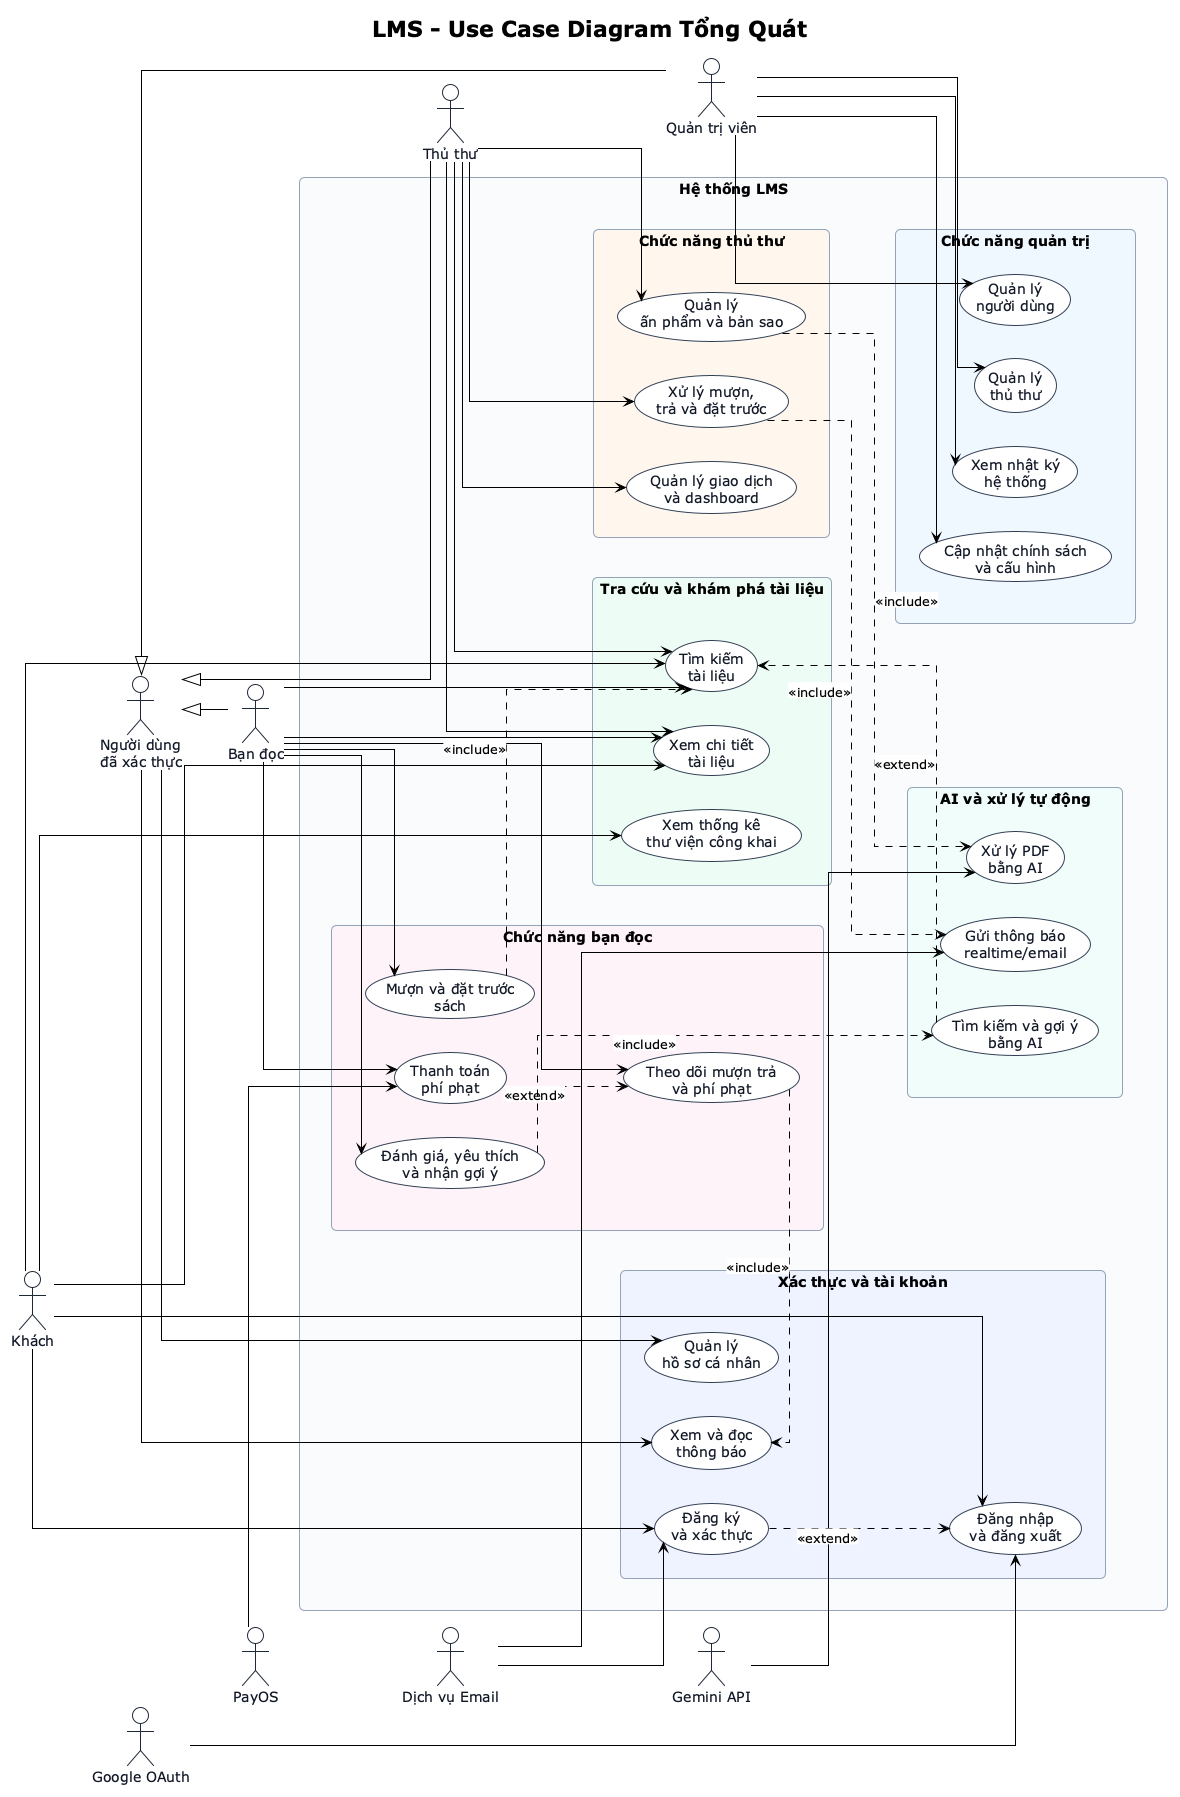
\includegraphics[width=\linewidth, height=0.82\textheight, keepaspectratio]{figures/ch05/usecase/overview.png}
 \caption{Biểu đồ Use Case tổng quát}
 \label{fig:usecase_overview}
\end{figure}

\begin{figure}[H]
 \centering
 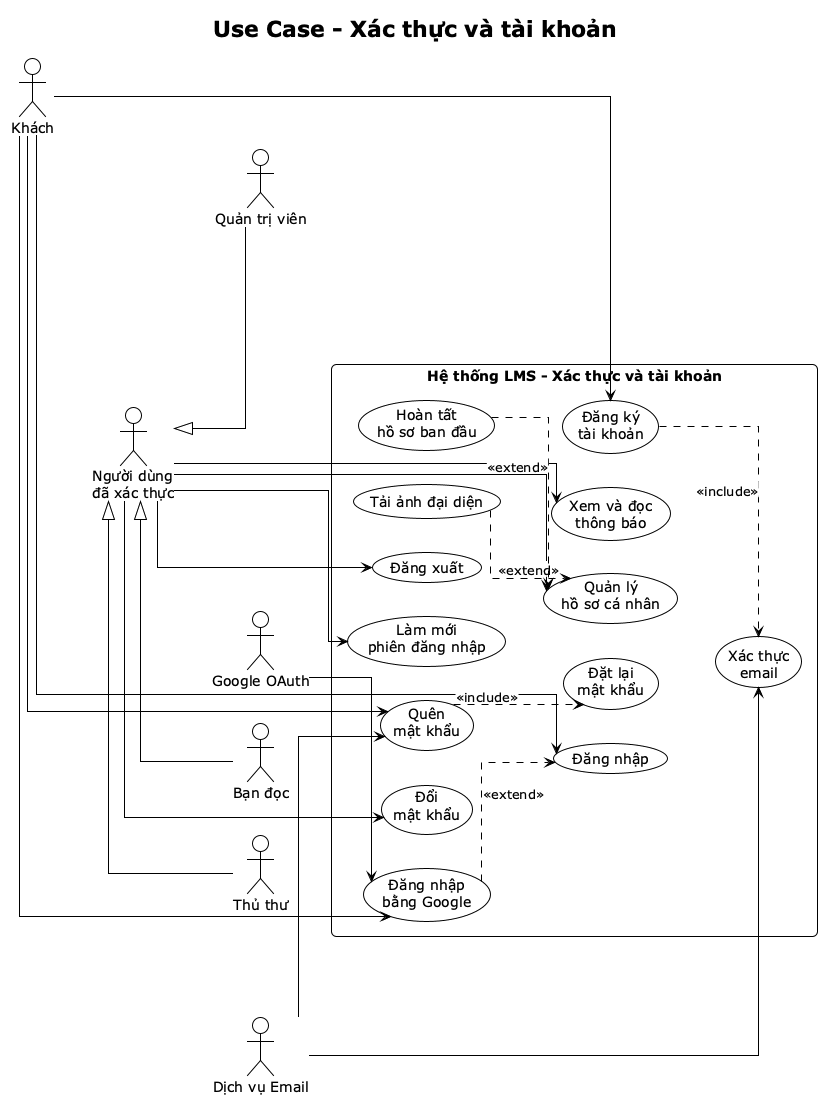
\includegraphics[width=\linewidth, height=0.78\textheight, keepaspectratio]{figures/ch05/usecase/modules/01_auth_account.png}
 \caption{Use Case module Xác thực và tài khoản}
 \label{fig:usecase_auth_account}
\end{figure}

\begin{figure}[H]
 \centering
 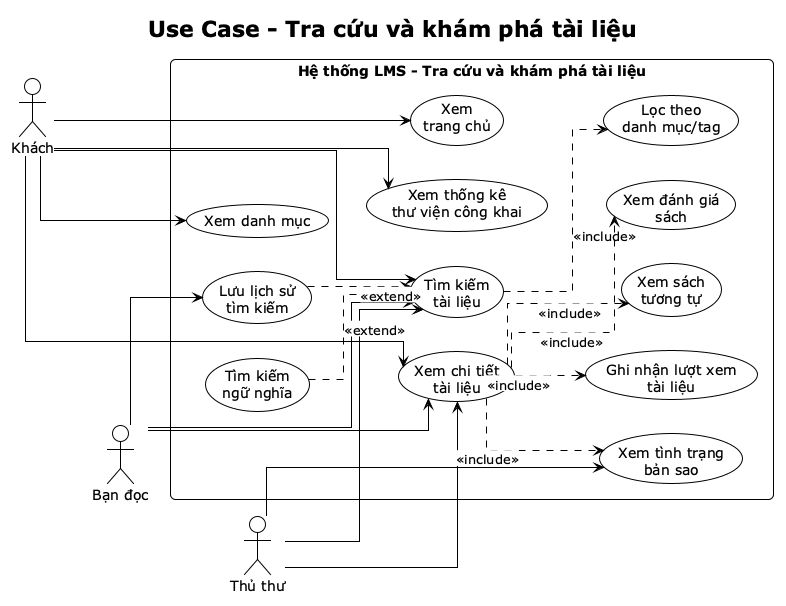
\includegraphics[width=\linewidth, height=0.78\textheight, keepaspectratio]{figures/ch05/usecase/modules/02_discovery_catalog.png}
 \caption{Use Case module Tra cứu và khám phá tài liệu}
 \label{fig:usecase_discovery_catalog}
\end{figure}

\begin{figure}[H]
 \centering
 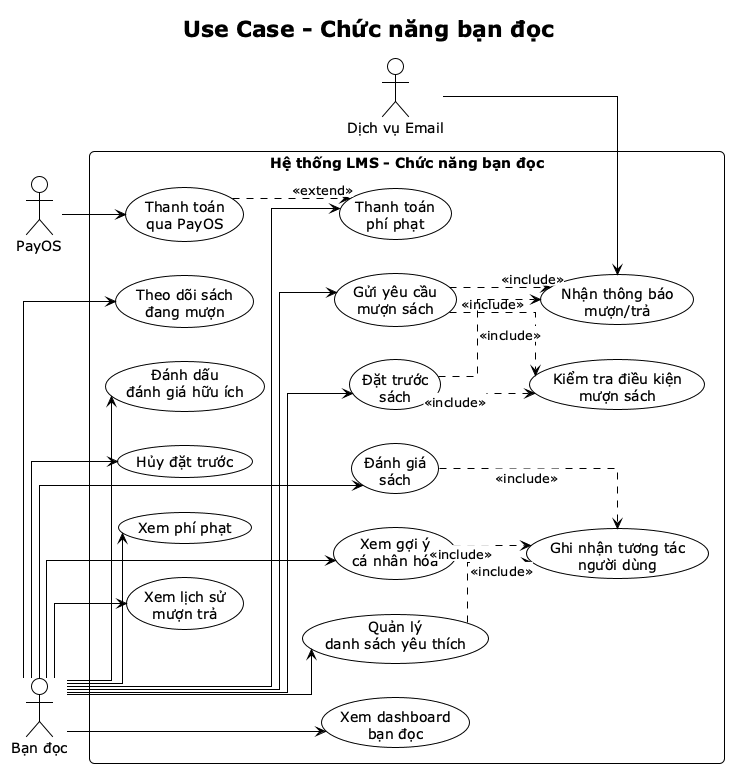
\includegraphics[width=\linewidth, height=0.78\textheight, keepaspectratio]{figures/ch05/usecase/modules/03_reader_services.png}
 \caption{Use Case module Chức năng bạn đọc}
 \label{fig:usecase_reader_services}
\end{figure}

\begin{figure}[H]
 \centering
 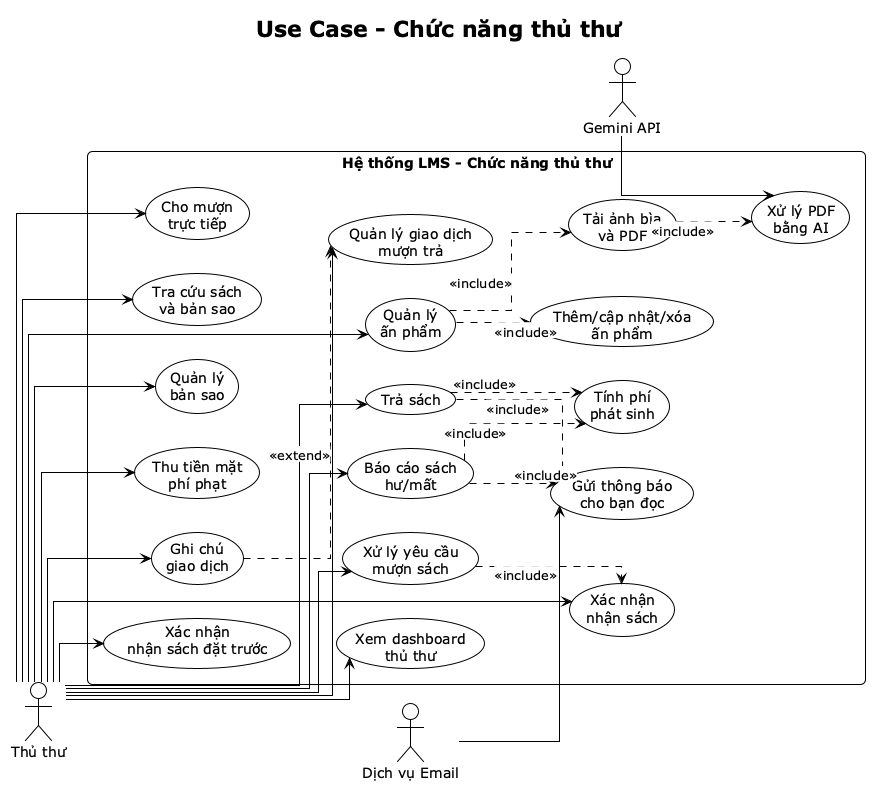
\includegraphics[width=\linewidth, height=0.78\textheight, keepaspectratio]{figures/ch05/usecase/modules/04_librarian_operations.png}
 \caption{Use Case module Chức năng thủ thư}
 \label{fig:usecase_librarian_operations}
\end{figure}

\begin{figure}[H]
 \centering
 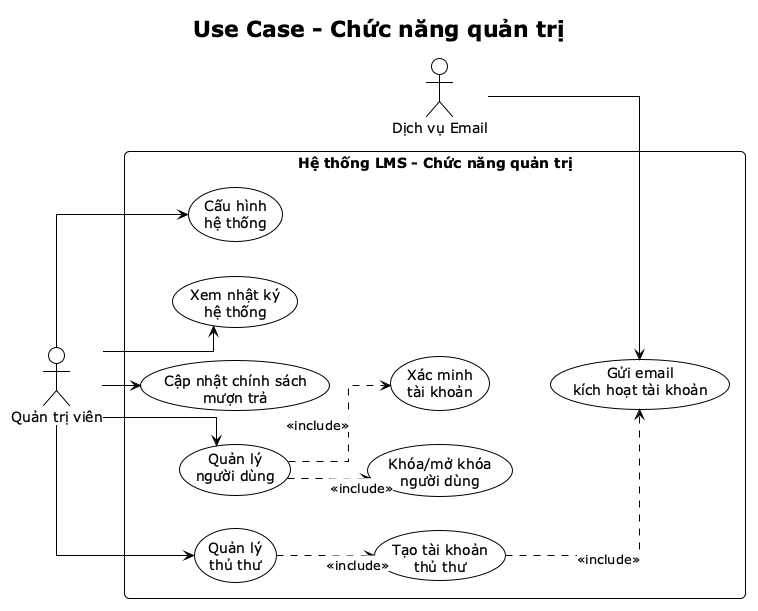
\includegraphics[width=\linewidth, height=0.78\textheight, keepaspectratio]{figures/ch05/usecase/modules/05_admin_management.png}
 \caption{Use Case module Chức năng quản trị}
 \label{fig:usecase_admin_management}
\end{figure}

\begin{figure}[H]
 \centering
 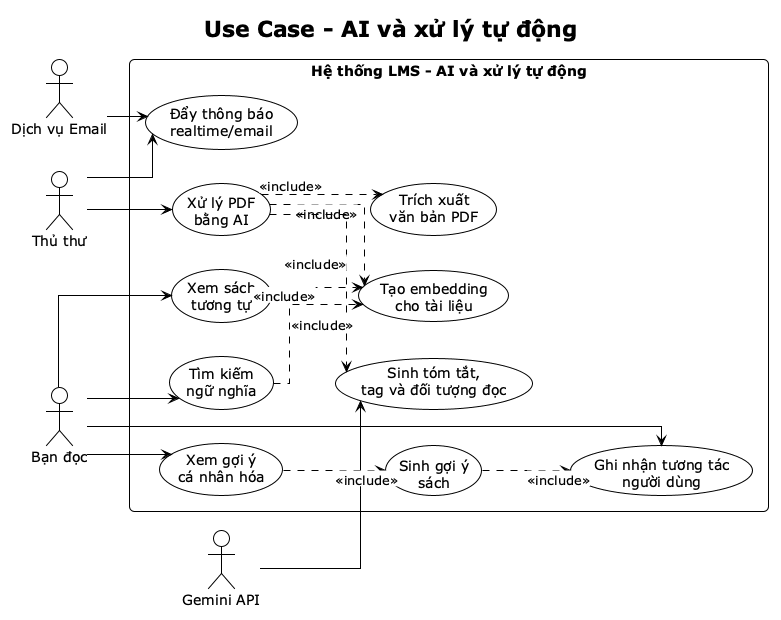
\includegraphics[width=\linewidth, height=0.78\textheight, keepaspectratio]{figures/ch05/usecase/modules/06_ai_automation.png}
 \caption{Use Case module AI và xử lý tự động}
 \label{fig:usecase_ai_automation}
\end{figure}

Sơ đồ tổng quát trong Hình~\ref{fig:usecase_overview} cho thấy ranh giới chính
của hệ thống: nhóm xác thực/tài khoản, nhóm tra cứu tài liệu, nhóm nghiệp vụ
bạn đọc, nhóm nghiệp vụ thủ thư, nhóm quản trị và nhóm AI tự động. Các sơ đồ
module từ Hình~\ref{fig:usecase_auth_account} đến
Hình~\ref{fig:usecase_ai_automation} làm rõ các quan hệ
\texttt{include}/\texttt{extend}: đăng ký bao gồm xác thực email; tìm kiếm có
thể mở rộng sang semantic search; mượn/đặt trước bao gồm kiểm tra điều kiện
mượn; upload PDF bao gồm xử lý AI; trả sách và báo hư/mất bao gồm tính phí và
gửi thông báo.

\begin{table}[H]
\centering
\caption{Đối chiếu nhóm Use Case với hiện thực hệ thống}
\label{tab:usecase_mapping_reality}
\begin{tabularx}{\linewidth}{|p{0.22\linewidth}|>{\raggedright\arraybackslash}X|>{\raggedright\arraybackslash}X|}
\hline
\textbf{Nhóm} & \textbf{Use case chính} & \textbf{Hiện thực tương ứng} \\
\hline
Xác thực và tài khoản & Đăng ký, xác thực email, đăng nhập thường, đăng nhập Google, refresh token, quên/đặt lại mật khẩu, hồ sơ, avatar, đổi mật khẩu, thông báo & Auth/User modules, OAuth2 Google, JWT/refresh token, email verification/reset password, profile API và notification API. \\
\hline
Tra cứu và khám phá tài liệu & Trang chủ, tìm kiếm catalog, semantic search, lọc danh mục/tag, chi tiết tài liệu, bản sao, đánh giá, sách tương tự, thống kê công khai & Public pages và catalog/recommendation API: \texttt{/api/v1/publications/search}, \texttt{/api/v1/ai/semantic-search}, \texttt{/api/v1/publications/\{id\}}, \texttt{/items}, \texttt{/ratings}, \texttt{/similar}. \\
\hline
Chức năng bạn đọc & Mượn, đặt trước, hủy đặt trước, theo dõi sách đang mượn, lịch sử mượn trả, phí phạt, PayOS, wishlist, rating, gợi ý cá nhân hóa & Reader pages, circulation/reservation/fine APIs, PayOS payment, wishlist/rating APIs và recommendation API. \\
\hline
Chức năng thủ thư & Quản lý ấn phẩm, bản sao, upload bìa/PDF, AI ETL, xử lý yêu cầu mượn, mượn trực tiếp, trả sách, báo hư/mất, ghi chú giao dịch, thu tiền mặt & Librarian pages, catalog/item APIs, presigned upload, backend AI gateway, circulation transaction APIs, fine cash payment và notification/email events. \\
\hline
Chức năng quản trị & Quản lý thủ thư, quản lý người dùng, khóa/mở khóa, xác minh tài khoản, chính sách mượn trả, nhật ký hệ thống & Admin pages và admin APIs: librarian/user management, circulation policy, audit log và account verification. \\
\hline
AI và xử lý tự động & Semantic search, recommendation, sách tương tự, xử lý PDF, trích xuất text, embedding, sinh summary/tag/audience, ghi nhận tương tác, realtime/email notification & AI service FastAPI/Celery, RabbitMQ, Gemini API, PostgreSQL pgvector, interaction tracking, Kafka/email/WebSocket notification. \\
\hline
\end{tabularx}
\end{table}

\subsubsection{Đặc tả các nhóm Use Case chính}
\begin{table}[H]
\centering
\caption{Bảng đặc tả UC-01: Xác thực và tài khoản}
\label{tab:uc_auth_account}
\begin{tabularx}{\linewidth}{|p{0.24\linewidth}|>{\raggedright\arraybackslash}X|}
\hline
\textbf{Thuộc tính} & \textbf{Mô tả chi tiết} \\
\hline
\textbf{Tên Use Case} & Xác thực và tài khoản \\
\hline
\textbf{Mã số} & UC-01 \\
\hline
\textbf{Tác nhân} & Khách, Người dùng đã xác thực, Bạn đọc, Thủ thư, Quản trị viên, Google OAuth, Dịch vụ Email \\
\hline
\textbf{Mô tả ngắn gọn} & Quản lý vòng đời đăng ký, xác thực email, đăng nhập thường/Google, refresh token, quên mật khẩu, đặt lại mật khẩu, hồ sơ cá nhân, avatar, đổi mật khẩu và thông báo người dùng. \\
\hline
\textbf{Tiền điều kiện} & Người dùng truy cập trang đăng ký/đăng nhập hoặc đã có phiên đăng nhập hợp lệ khi thao tác với hồ sơ và thông báo. \\
\hline
\textbf{Hậu điều kiện} & \textbf{Thành công:} Tài khoản được tạo/xác thực, phiên đăng nhập được cấp, thông tin hồ sơ hoặc trạng thái thông báo được cập nhật. \newline \textbf{Thất bại:} Hệ thống giữ nguyên dữ liệu và trả thông báo lỗi xác thực, validation hoặc quyền truy cập. \\
\hline
\textbf{Luồng chính} &
1. Khách đăng ký tài khoản hoặc đăng nhập bằng email/mật khẩu hoặc Google OAuth. \newline
2. Backend kiểm tra dữ liệu, mã hóa mật khẩu, tạo token hoặc xử lý callback OAuth2. \newline
3. Với tài khoản mới hoặc quên mật khẩu, hệ thống gửi email xác thực/đặt lại mật khẩu. \newline
4. Người dùng đã xác thực quản lý hồ sơ, avatar, mật khẩu và đọc thông báo. \newline
5. Hệ thống cập nhật trạng thái tài khoản, refresh token, hồ sơ hoặc notification tương ứng. \\
\hline
\textbf{Luồng thay thế} &
\textbf{Email đã tồn tại hoặc token hết hạn:} hệ thống trả lỗi và yêu cầu người dùng nhập lại hoặc gửi lại email. \newline
\textbf{OAuth2 không hợp lệ:} backend từ chối callback và chuyển người dùng về luồng đăng nhập. \\
\hline
\end{tabularx}
\end{table}

\begin{table}[H]
\centering
\caption{Bảng đặc tả UC-02: Tra cứu và khám phá tài liệu}
\label{tab:uc_discovery_catalog}
\begin{tabularx}{\linewidth}{|p{0.24\linewidth}|>{\raggedright\arraybackslash}X|}
\hline
\textbf{Thuộc tính} & \textbf{Mô tả chi tiết} \\
\hline
\textbf{Tên Use Case} & Tra cứu và khám phá tài liệu \\
\hline
\textbf{Mã số} & UC-02 \\
\hline
\textbf{Tác nhân} & Khách, Bạn đọc, Thủ thư \\
\hline
\textbf{Mô tả ngắn gọn} & Cho phép người dùng xem trang chủ, tìm kiếm catalog, tìm kiếm ngữ nghĩa, lọc theo danh mục/tag, xem chi tiết tài liệu, bản sao, đánh giá, sách tương tự và thống kê công khai. \\
\hline
\textbf{Tiền điều kiện} & Catalog có dữ liệu ấn phẩm; với semantic search, tài liệu liên quan đã có vector embedding trong AI database. \\
\hline
\textbf{Hậu điều kiện} & \textbf{Thành công:} Danh sách hoặc chi tiết ấn phẩm được hiển thị, lịch sử tìm kiếm/lượt xem được ghi nhận khi phù hợp. \newline \textbf{Thất bại:} Hệ thống hiển thị trạng thái không có kết quả hoặc thông báo lỗi dịch vụ AI. \\
\hline
\textbf{Luồng chính} &
1. Người dùng nhập từ khóa, chọn bộ lọc hoặc nhập truy vấn tự nhiên. \newline
2. Frontend gọi API catalog search hoặc semantic search. \newline
3. Backend lọc catalog bằng PostgreSQL hoặc chuyển truy vấn sang AI service để tìm vector gần nhất. \newline
4. Hệ thống trả danh sách ấn phẩm, trạng thái bản sao, rating, AI summary và sách tương tự. \newline
5. Khi người dùng mở chi tiết, hệ thống ghi nhận lượt xem và hiển thị metadata liên quan. \\
\hline
\textbf{Luồng thay thế} &
\textbf{Không có kết quả:} giao diện hiển thị trạng thái rỗng và giữ bộ lọc để người dùng điều chỉnh. \newline
\textbf{AI service không sẵn sàng:} hệ thống vẫn có thể dùng tìm kiếm catalog thông thường. \\
\hline
\end{tabularx}
\end{table}

\begin{table}[H]
\centering
\caption{Bảng đặc tả UC-03: Chức năng bạn đọc}
\label{tab:uc_reader_services}
\begin{tabularx}{\linewidth}{|p{0.24\linewidth}|>{\raggedright\arraybackslash}X|}
\hline
\textbf{Thuộc tính} & \textbf{Mô tả chi tiết} \\
\hline
\textbf{Tên Use Case} & Chức năng bạn đọc \\
\hline
\textbf{Mã số} & UC-03 \\
\hline
\textbf{Tác nhân} & Bạn đọc, PayOS, Dịch vụ Email \\
\hline
\textbf{Mô tả ngắn gọn} & Cho phép bạn đọc xem dashboard, gửi yêu cầu mượn, đặt trước, hủy đặt trước, theo dõi sách đang mượn, xem lịch sử, xem/thanh toán phí phạt, quản lý wishlist, đánh giá sách và nhận gợi ý cá nhân hóa. \\
\hline
\textbf{Tiền điều kiện} & Bạn đọc đã đăng nhập, tài khoản hoạt động và không vi phạm các điều kiện nghiệp vụ đang được kiểm tra như giới hạn mượn hoặc phí phạt chưa thanh toán. \\
\hline
\textbf{Hậu điều kiện} & \textbf{Thành công:} Giao dịch mượn/đặt trước/phí phạt/wishlist/rating được cập nhật; tương tác người dùng được ghi nhận cho recommendation. \newline \textbf{Thất bại:} Hệ thống giữ nguyên trạng thái và trả thông báo lỗi. \\
\hline
\textbf{Luồng chính} &
1. Bạn đọc xem dashboard và mở chi tiết tài liệu. \newline
2. Bạn đọc gửi yêu cầu mượn hoặc đặt trước; backend kiểm tra chính sách mượn và trạng thái bản sao. \newline
3. Hệ thống tạo giao dịch hoặc reservation, gửi thông báo/email khi cần. \newline
4. Bạn đọc theo dõi sách đang mượn, lịch sử, phí phạt và thanh toán qua PayOS nếu chọn thanh toán online. \newline
5. Bạn đọc thêm wishlist, đánh giá sách hoặc xem gợi ý cá nhân hóa; hệ thống ghi nhận tương tác. \\
\hline
\textbf{Luồng thay thế} &
\textbf{Không đủ điều kiện mượn:} hệ thống từ chối yêu cầu và nêu lý do. \newline
\textbf{Thanh toán PayOS thất bại:} phí phạt giữ trạng thái chưa thanh toán để xử lý lại hoặc thu tiền mặt. \\
\hline
\end{tabularx}
\end{table}

\begin{table}[H]
\centering
\caption{Bảng đặc tả UC-04: Chức năng thủ thư}
\label{tab:uc_librarian_operations}
\begin{tabularx}{\linewidth}{|p{0.24\linewidth}|>{\raggedright\arraybackslash}X|}
\hline
\textbf{Thuộc tính} & \textbf{Mô tả chi tiết} \\
\hline
\textbf{Tên Use Case} & Chức năng thủ thư \\
\hline
\textbf{Mã số} & UC-04 \\
\hline
\textbf{Tác nhân} & Thủ thư, Dịch vụ Email, Gemini API \\
\hline
\textbf{Mô tả ngắn gọn} & Thủ thư quản lý ấn phẩm, bản sao, file bìa/PDF, kích hoạt AI ETL, xử lý mượn/trả/đặt trước, báo hư/mất, ghi chú giao dịch, thu tiền mặt và gửi thông báo cho bạn đọc. \\
\hline
\textbf{Tiền điều kiện} & Thủ thư đã đăng nhập và có quyền thao tác với catalog/circulation. Các barcode, publication hoặc transaction liên quan tồn tại trong hệ thống. \\
\hline
\textbf{Hậu điều kiện} & \textbf{Thành công:} Catalog, bản sao, giao dịch, phí phạt hoặc trạng thái AI ETL được cập nhật; thông báo/email được gửi khi nghiệp vụ yêu cầu. \newline \textbf{Thất bại:} Dữ liệu không đổi và hệ thống hiển thị lỗi. \\
\hline
\textbf{Luồng chính} &
1. Thủ thư quản lý metadata ấn phẩm, bản sao và upload file bìa/PDF. \newline
2. Khi upload PDF, backend lưu URL tài liệu và kích hoạt AI ETL để xử lý nội dung. \newline
3. Thủ thư tra cứu bạn đọc, barcode, yêu cầu mượn hoặc reservation. \newline
4. Hệ thống xử lý mượn trực tiếp, xác nhận nhận sách, trả sách, báo hư/mất và tính phí phát sinh. \newline
5. Thủ thư theo dõi dashboard/giao dịch, ghi chú nghiệp vụ và thu tiền mặt khi cần. \\
\hline
\textbf{Luồng thay thế} &
\textbf{Barcode/giao dịch không hợp lệ:} hệ thống từ chối cập nhật. \newline
\textbf{AI service lỗi:} trạng thái ETL ghi nhận thất bại, catalog vẫn lưu metadata thủ công để thủ thư xử lý lại sau. \\
\hline
\end{tabularx}
\end{table}

\begin{table}[H]
\centering
\caption{Bảng đặc tả UC-05: Chức năng quản trị}
\label{tab:dt_admin_management}
\begin{tabularx}{\linewidth}{|p{0.24\linewidth}|>{\raggedright\arraybackslash}X|}
\hline
\textbf{Thuộc tính} & \textbf{Mô tả chi tiết} \\
\hline
\textbf{Tên Use Case} & Chức năng quản trị \\
\hline
\textbf{Mã số} & UC-05 \\
\hline
\textbf{Tác nhân} & Quản trị viên, Dịch vụ Email \\
\hline
\textbf{Mô tả ngắn gọn} & Quản trị viên quản lý tài khoản thủ thư, người dùng, trạng thái khóa/mở khóa, xác minh tài khoản, chính sách mượn trả, nhật ký hệ thống và cấu hình hệ thống. \\
\hline
\textbf{Tiền điều kiện} & Quản trị viên đã đăng nhập với vai trò admin. \\
\hline
\textbf{Hậu điều kiện} & Tài khoản, chính sách hoặc dữ liệu audit/config được cập nhật theo thao tác hợp lệ; email kích hoạt được gửi khi tạo tài khoản thủ thư. \\
\hline
\textbf{Luồng chính} & 1. Admin mở màn hình quản trị. \newline
2. Admin tạo/cập nhật tài khoản thủ thư hoặc quản lý người dùng. \newline
3. Hệ thống kiểm tra quyền, cập nhật trạng thái người dùng, gửi email kích hoạt nếu cần. \newline
4. Admin cập nhật chính sách mượn trả hoặc xem nhật ký hệ thống để kiểm soát vận hành. \\
\hline
\textbf{Luồng thay thế} & Nếu dữ liệu không hợp lệ hoặc admin không đủ quyền cho thao tác cụ thể, hệ thống từ chối và ghi nhận lỗi phù hợp. \\
\hline
\end{tabularx}
\end{table}

\begin{table}[H]
\centering
\caption{Bảng đặc tả UC-06: AI và xử lý tự động}
\label{tab:dt_ai_automation}
\begin{tabularx}{\linewidth}{|p{0.24\linewidth}|>{\raggedright\arraybackslash}X|}
\hline
\textbf{Thuộc tính} & \textbf{Mô tả chi tiết} \\
\hline
\textbf{Tên Use Case} & AI và xử lý tự động \\
\hline
\textbf{Mã số} & UC-06 \\
\hline
\textbf{Tác nhân} & Bạn đọc, Thủ thư, Gemini API, Dịch vụ Email \\
\hline
\textbf{Mô tả ngắn gọn} & AI service hỗ trợ semantic search, sách tương tự, recommendation, xử lý PDF, trích xuất text, tạo embedding, sinh summary/tag/audience, ghi nhận tương tác và đẩy thông báo realtime/email. \\
\hline
\textbf{Tiền điều kiện} & Tài liệu đã được upload hoặc người dùng có truy vấn/tương tác cần xử lý. AI service có thể truy cập database, RabbitMQ, model embedding và Gemini API khi cần sinh metadata. \\
\hline
\textbf{Hậu điều kiện} & Vector, metadata AI, recommendation cache hoặc notification được cập nhật. Nếu Gemini không khả dụng, pipeline ghi lỗi hoặc dùng fallback theo logic ETL. \\
\hline
\textbf{Luồng chính} & 1. Backend gửi yêu cầu xử lý tài liệu hoặc truy vấn AI. \newline
2. AI API nhận request, Celery worker xử lý job qua RabbitMQ. \newline
3. Worker trích xuất PDF, tạo embedding, ghi vector, gọi Gemini để sinh summary/tag/audience. \newline
4. Kết quả được ghi về PostgreSQL/pgvector và callback trạng thái về backend. \newline
5. Semantic search/recommendation dùng dữ liệu vector và tương tác người dùng để trả kết quả. \\
\hline
\textbf{Luồng thay thế} & Nếu LLM lỗi/quota, hệ thống ghi trạng thái thất bại hoặc dùng deterministic fallback; nếu chưa có vector, semantic search bỏ qua tài liệu đó cho đến khi ETL hoàn tất. \\
\hline
\end{tabularx}
\end{table}

\subsection{Mô hình lớp (Class diagram)}
\label{subsec:ClassDiagram}

Class diagram trong Hình~\ref{fig:class_diagram_lms} mô tả các lớp domain
chính của hệ thống theo nhóm User/Authentication, Catalog, Circulation,
Recommendation/AI và Payment/Notification. Sơ đồ tập trung vào entity, thuộc
tính nghiệp vụ, phương thức domain và quan hệ giữa các lớp, giúp liên kết phần
phân tích use case với thiết kế dữ liệu và cấu trúc backend.

\begin{figure}[H]
 \centering
 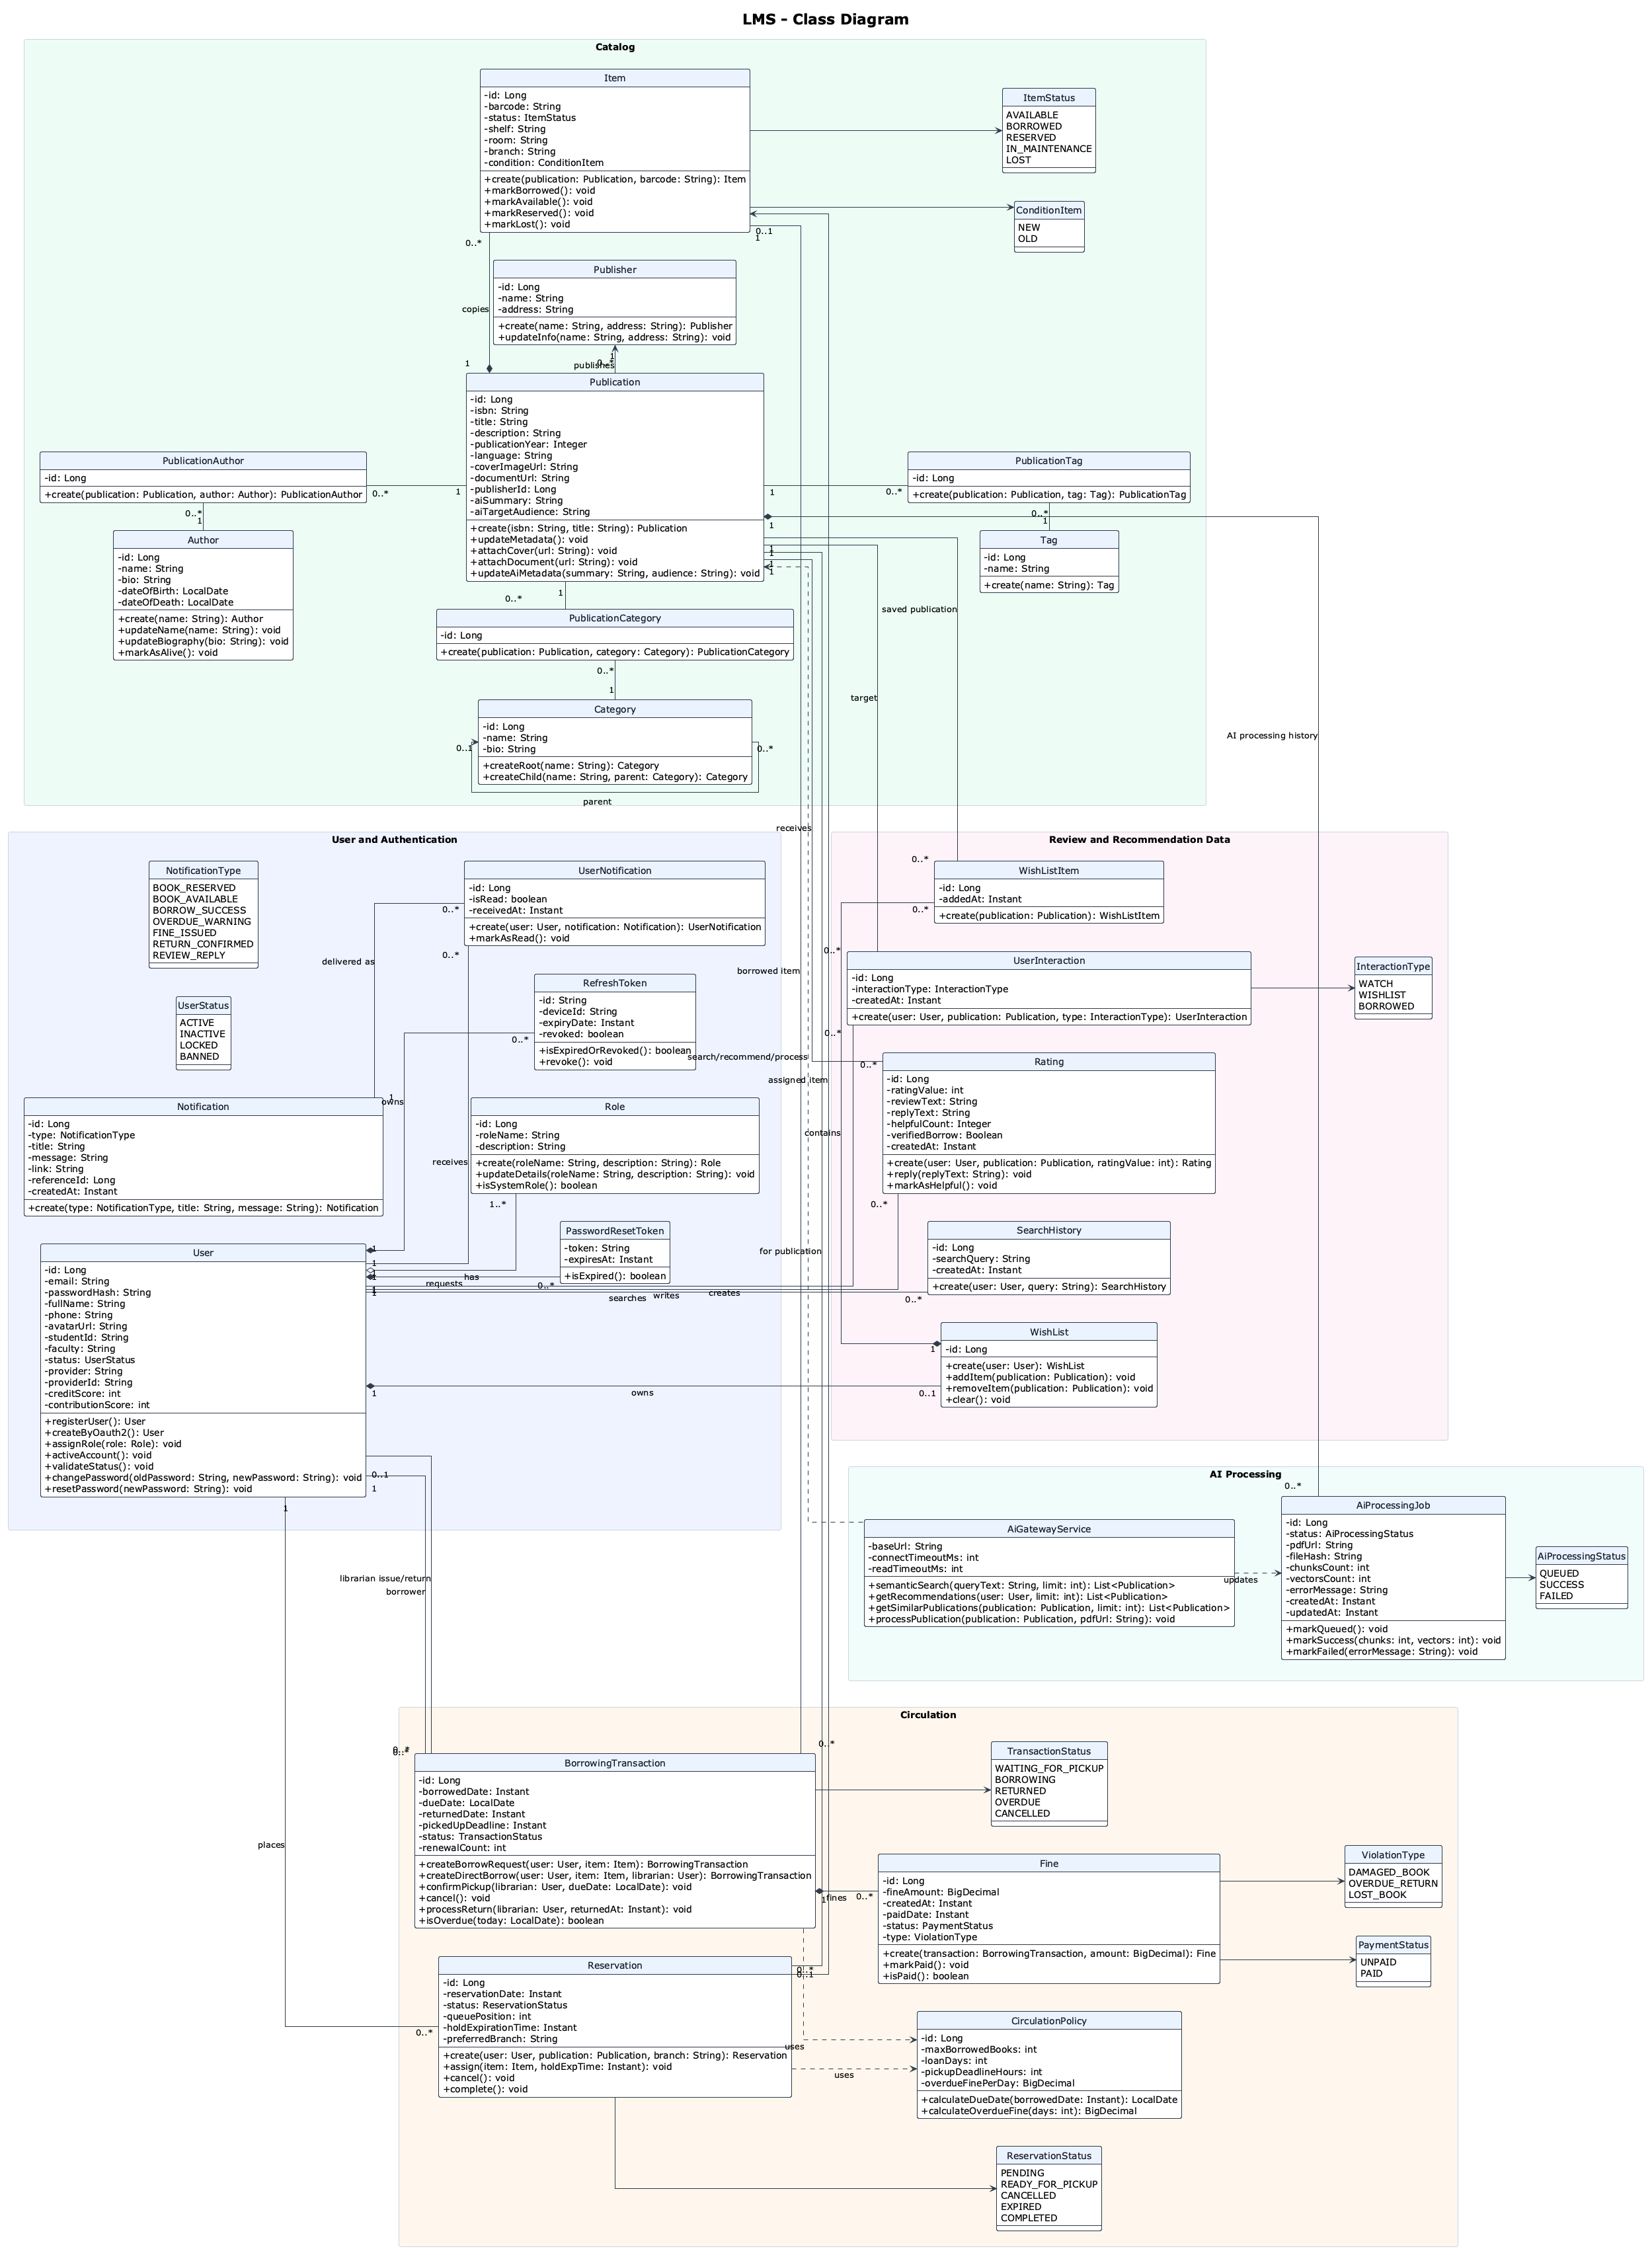
\includegraphics[width=\linewidth, height=0.9\textheight, keepaspectratio]{figures/ch05/class/classdiagram.png}
 \caption{Class diagram tổng quát của hệ thống}
 \label{fig:class_diagram_lms}
\end{figure}

\subsection{Mô hình hoá quy trình nghiệp vụ (Activity diagram)}
\label{subsec:ActivityDiagram}

Các activity diagram trong phần này mô tả những luồng nghiệp vụ đã được hiện thực thành màn hình và API. Riêng chức năng \textbf{gia hạn sách} không được đưa vào phạm vi hiện tại vì backend chưa có use case/controller hoàn chỉnh cho thao tác này; hệ thống chỉ lưu \texttt{renewal\_count} trong mô hình dữ liệu để có thể mở rộng về sau.

% + Đăng ký tài khoản
\begin{figure}[htbp]
 \centering
 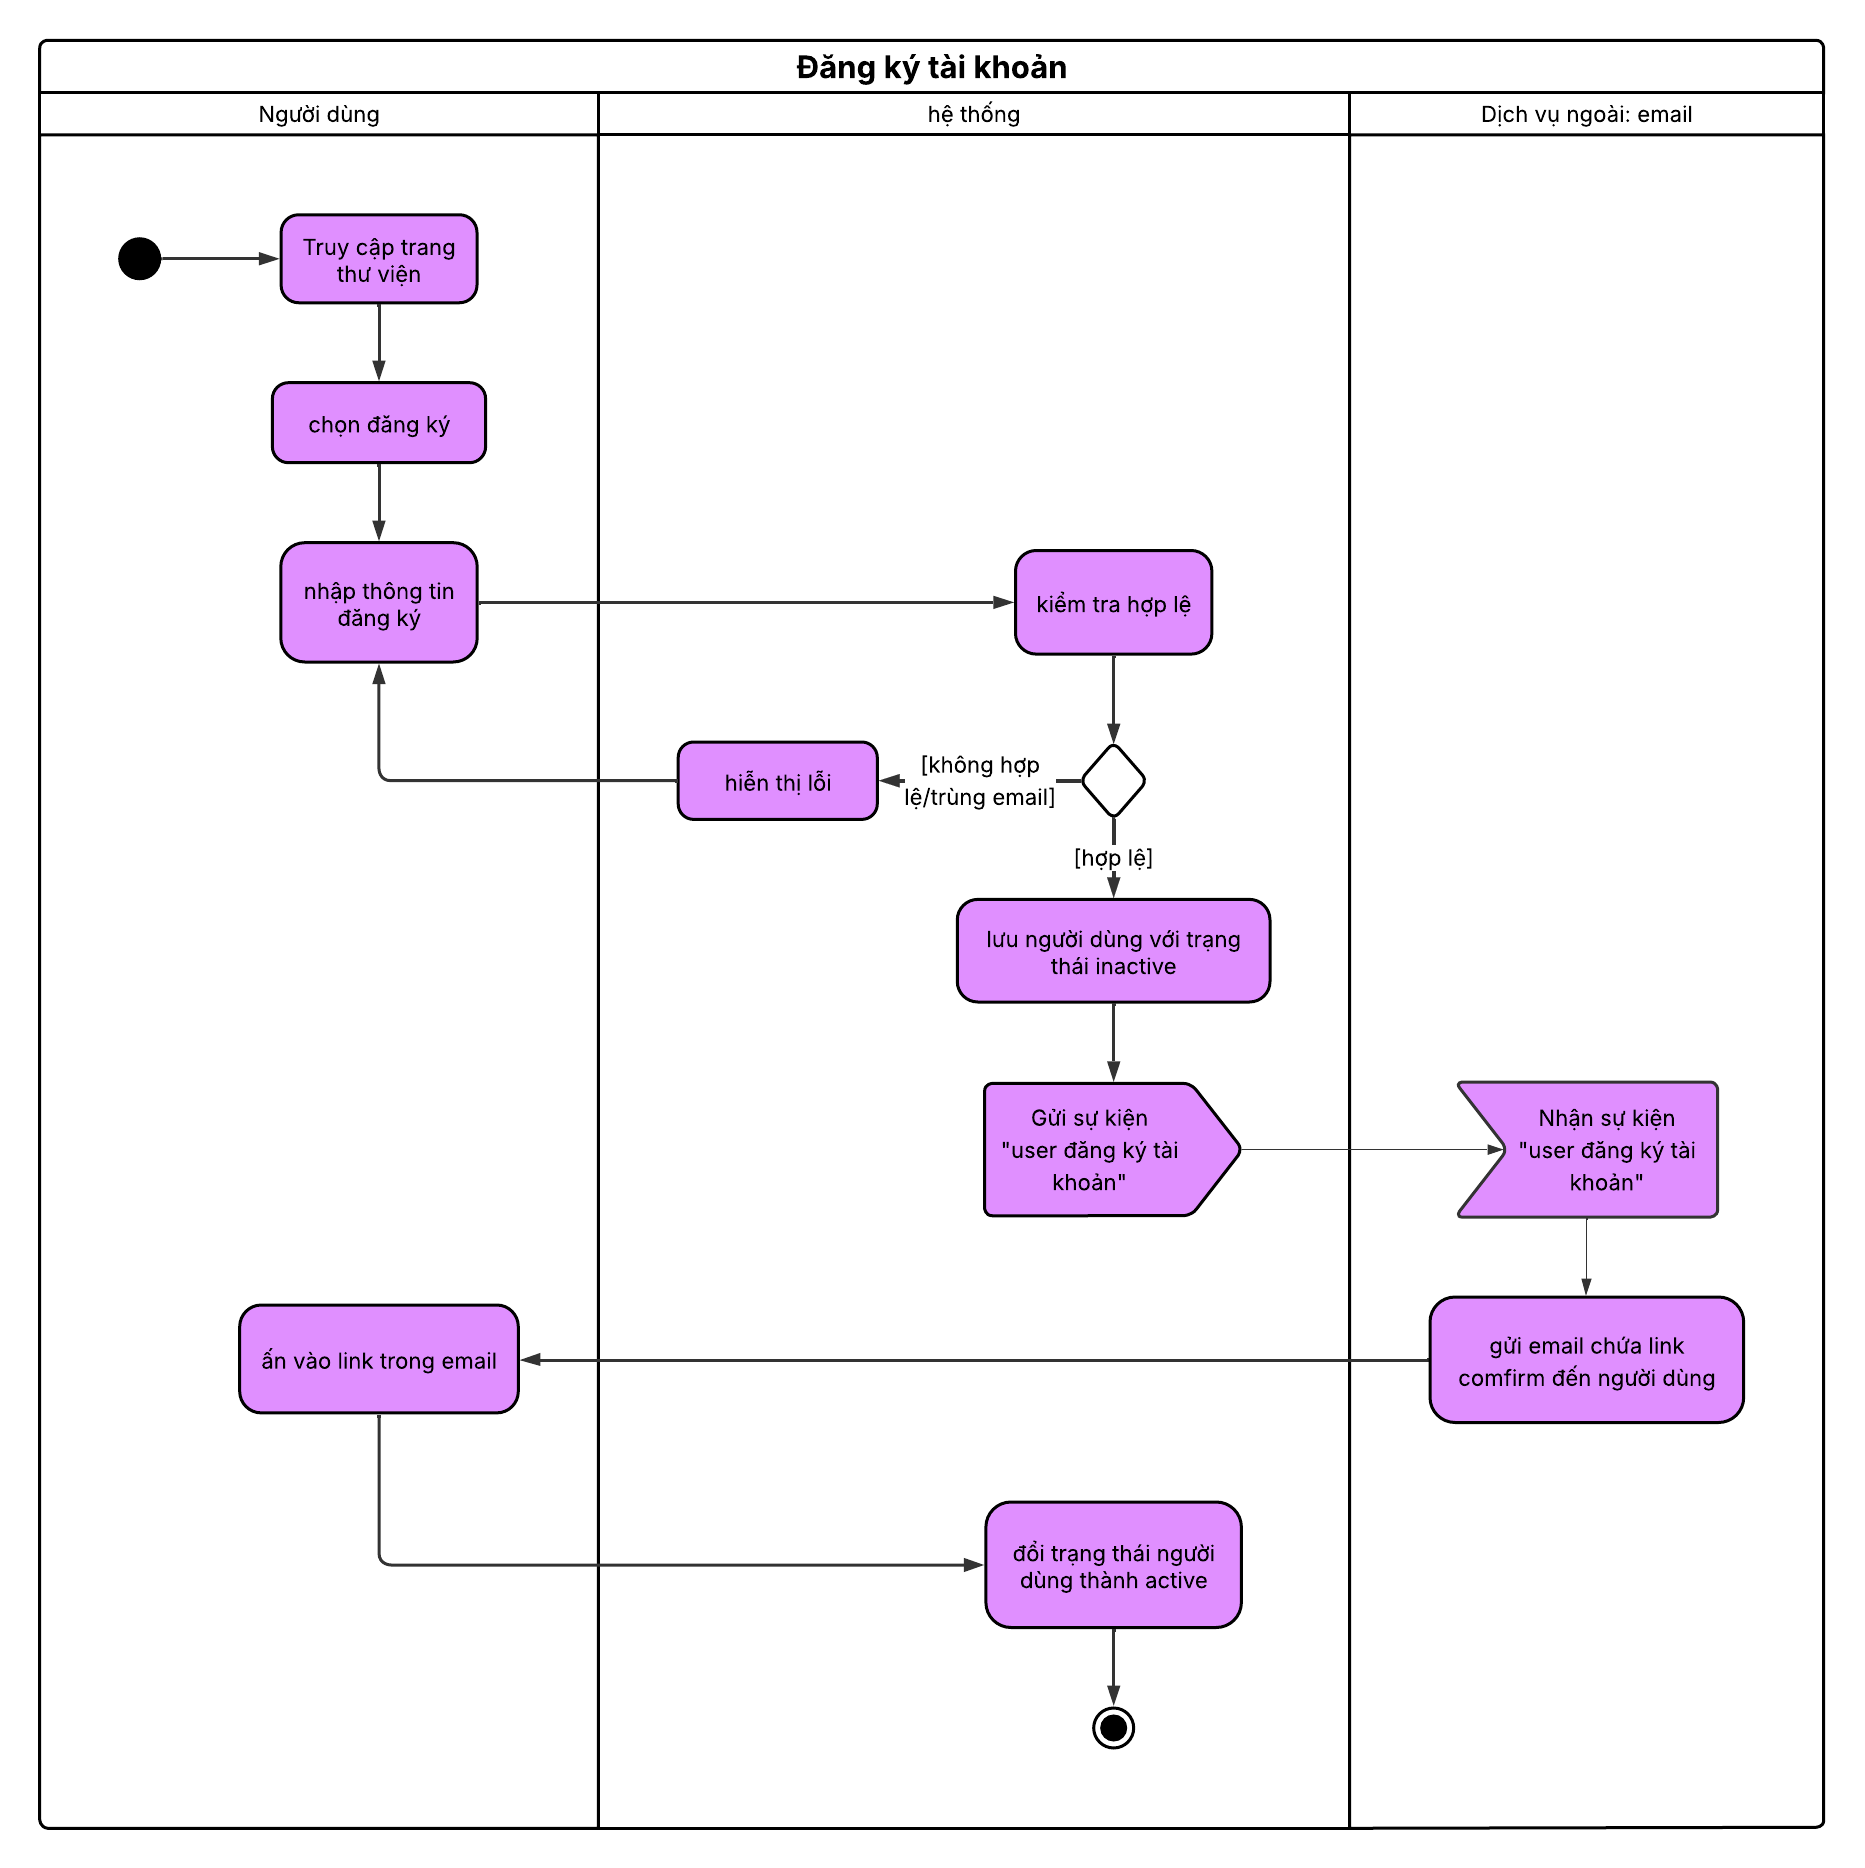
\includegraphics[width=1\linewidth]{figures/ch05/activity/sign_up.png}
 \caption{Đăng ký tài khoản — Activity Diagram}
 \label{fig:signup}
\end{figure}

% + Đăng nhập tài khoản
\begin{figure}[htbp]
 \centering
 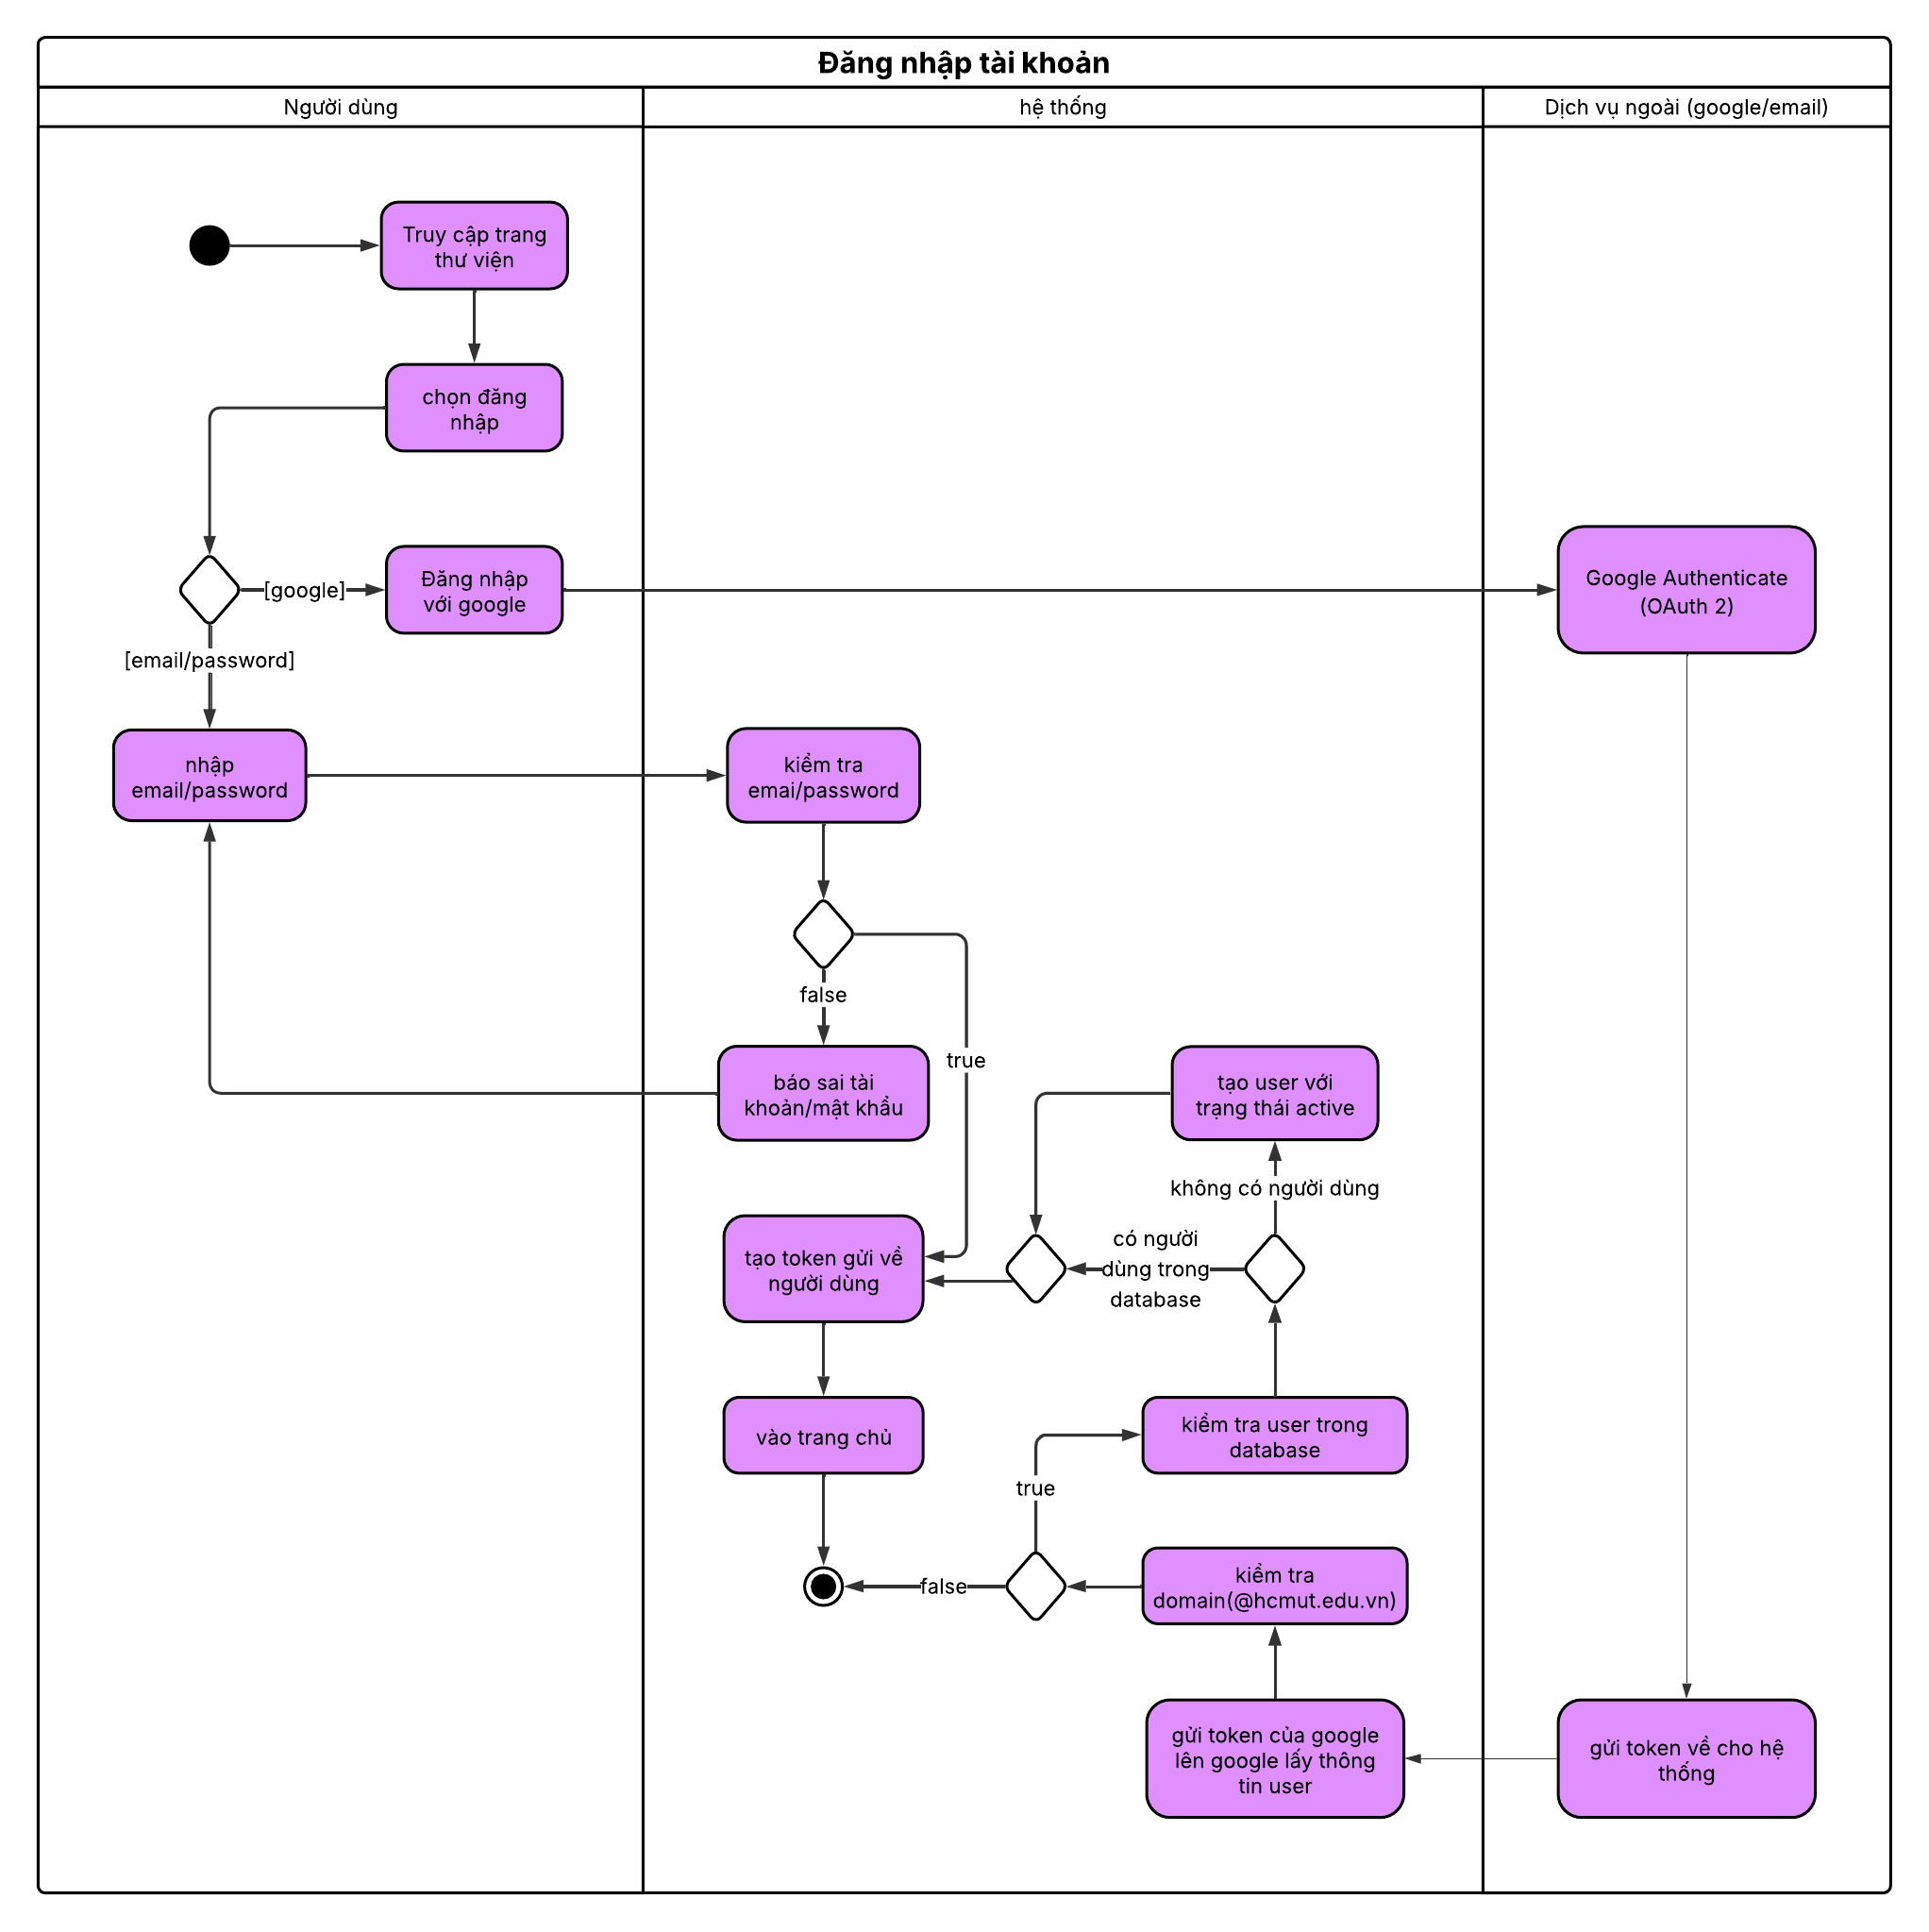
\includegraphics[width=1\linewidth]{figures/ch05/activity/login.png}
 \caption{Đăng nhập tài khoản — Activity Diagram}
 \label{fig:signin}
\end{figure}

% + Tìm kiếm sách:
\begin{figure}[htbp]
 \centering
 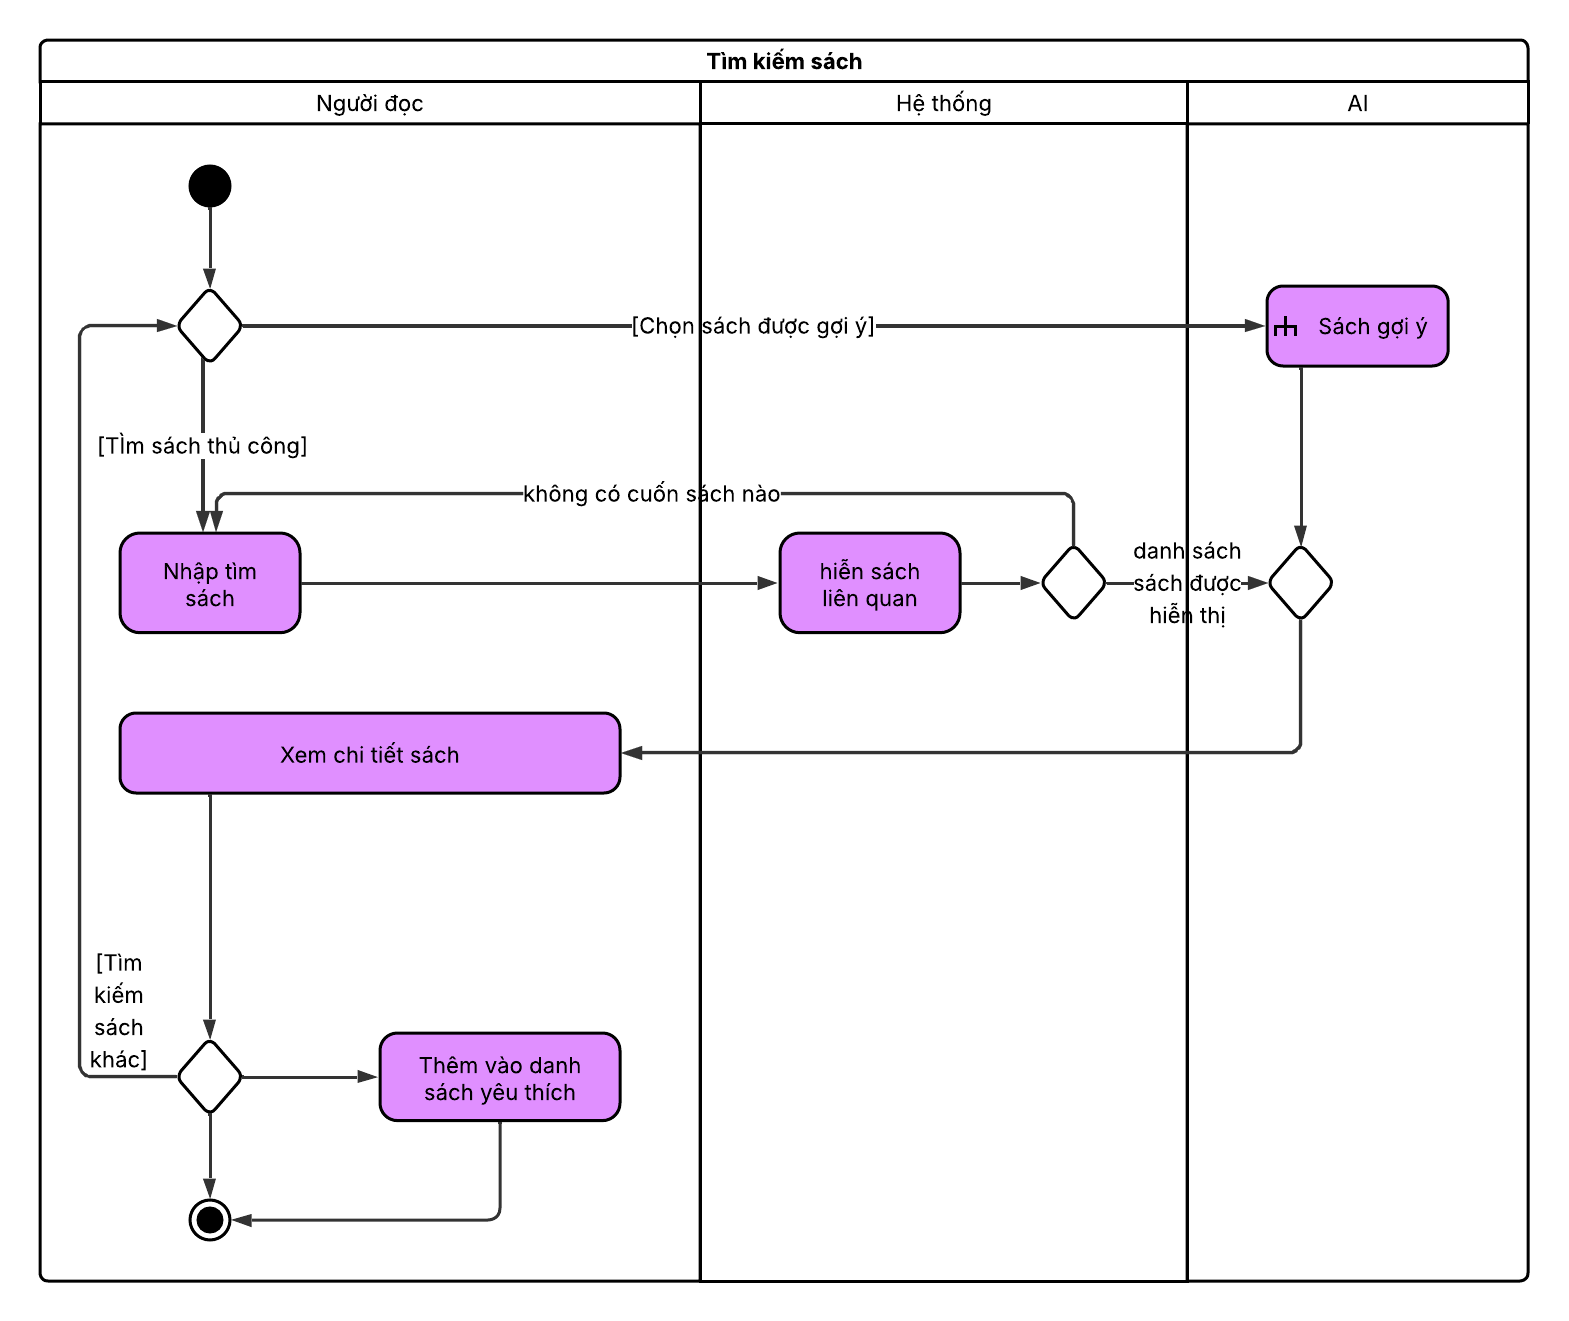
\includegraphics[width=\linewidth]{figures/ch05/activity/search_book.png}
 \caption{Tìm kiếm sách — Activity Diagram}
 \label{fig:search-book}
\end{figure}

% + Gợi ý sách:
\begin{figure}[htbp]
 \centering
 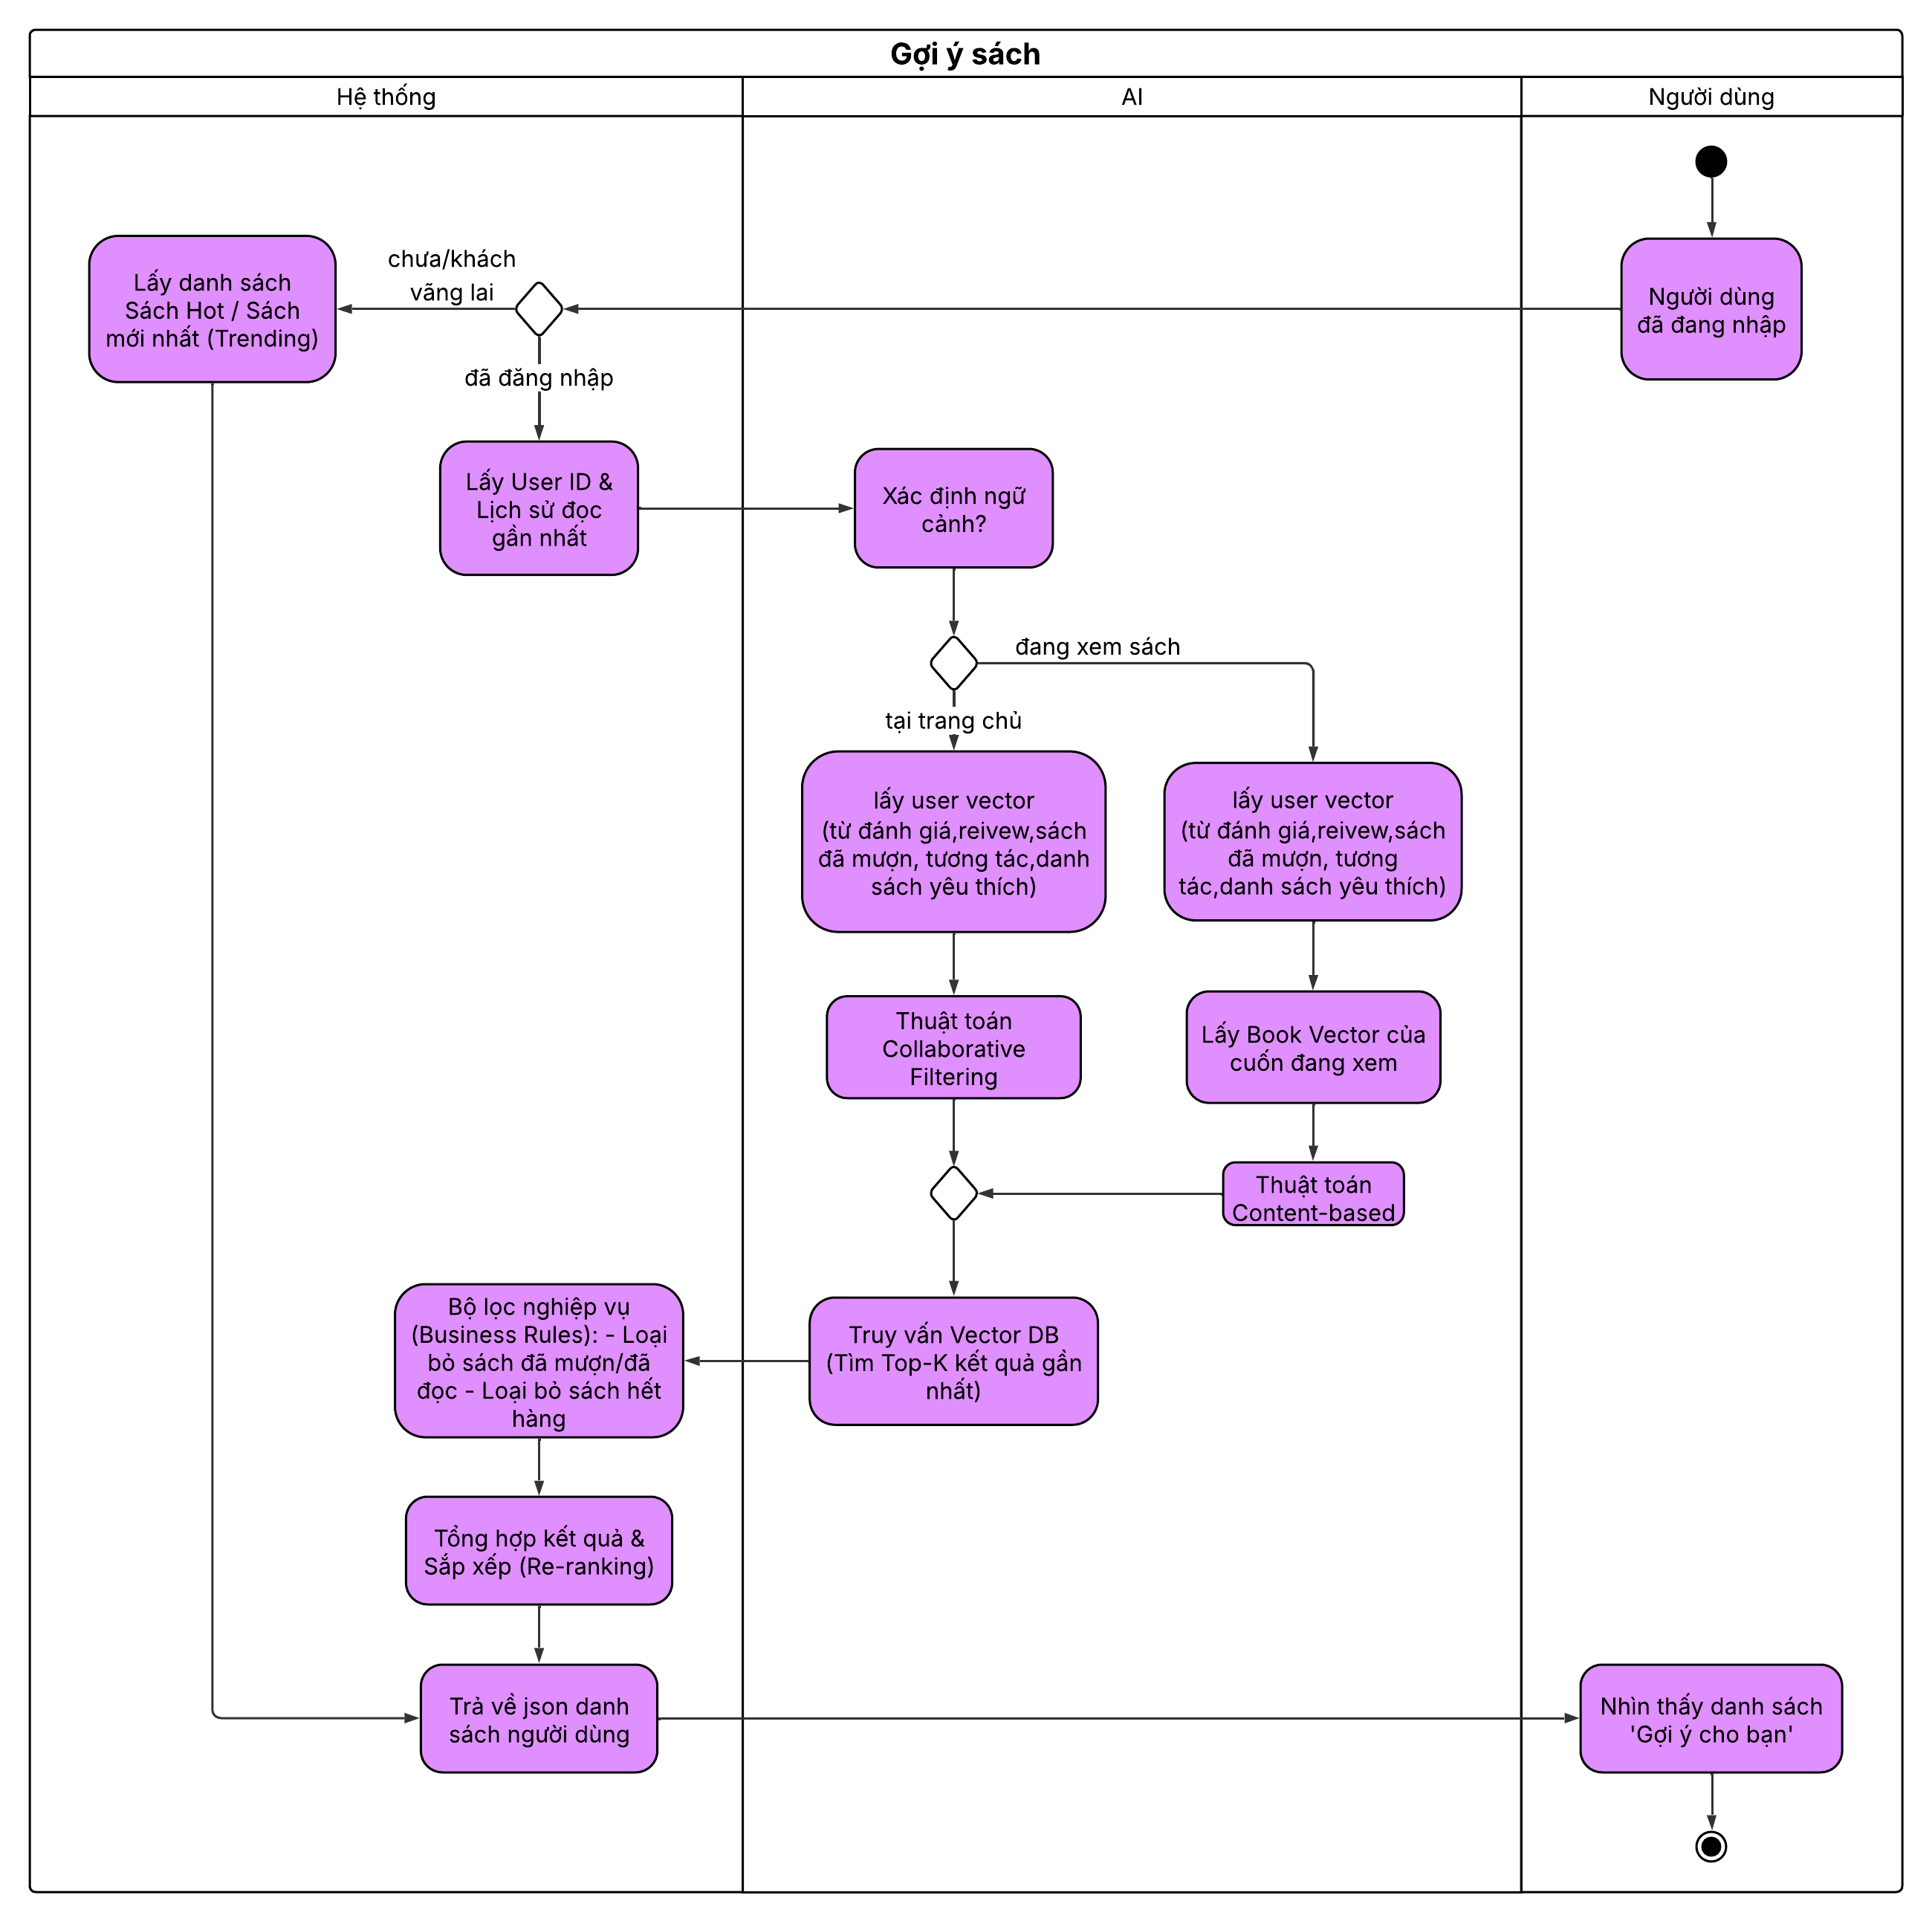
\includegraphics[width=\linewidth]{figures/ch05/activity/suggest_book.png}
 \caption{Gợi ý sách — Activity Diagram}
 \label{fig:suggestion}
\end{figure}

\begin{figure}[htbp]
 \centering
 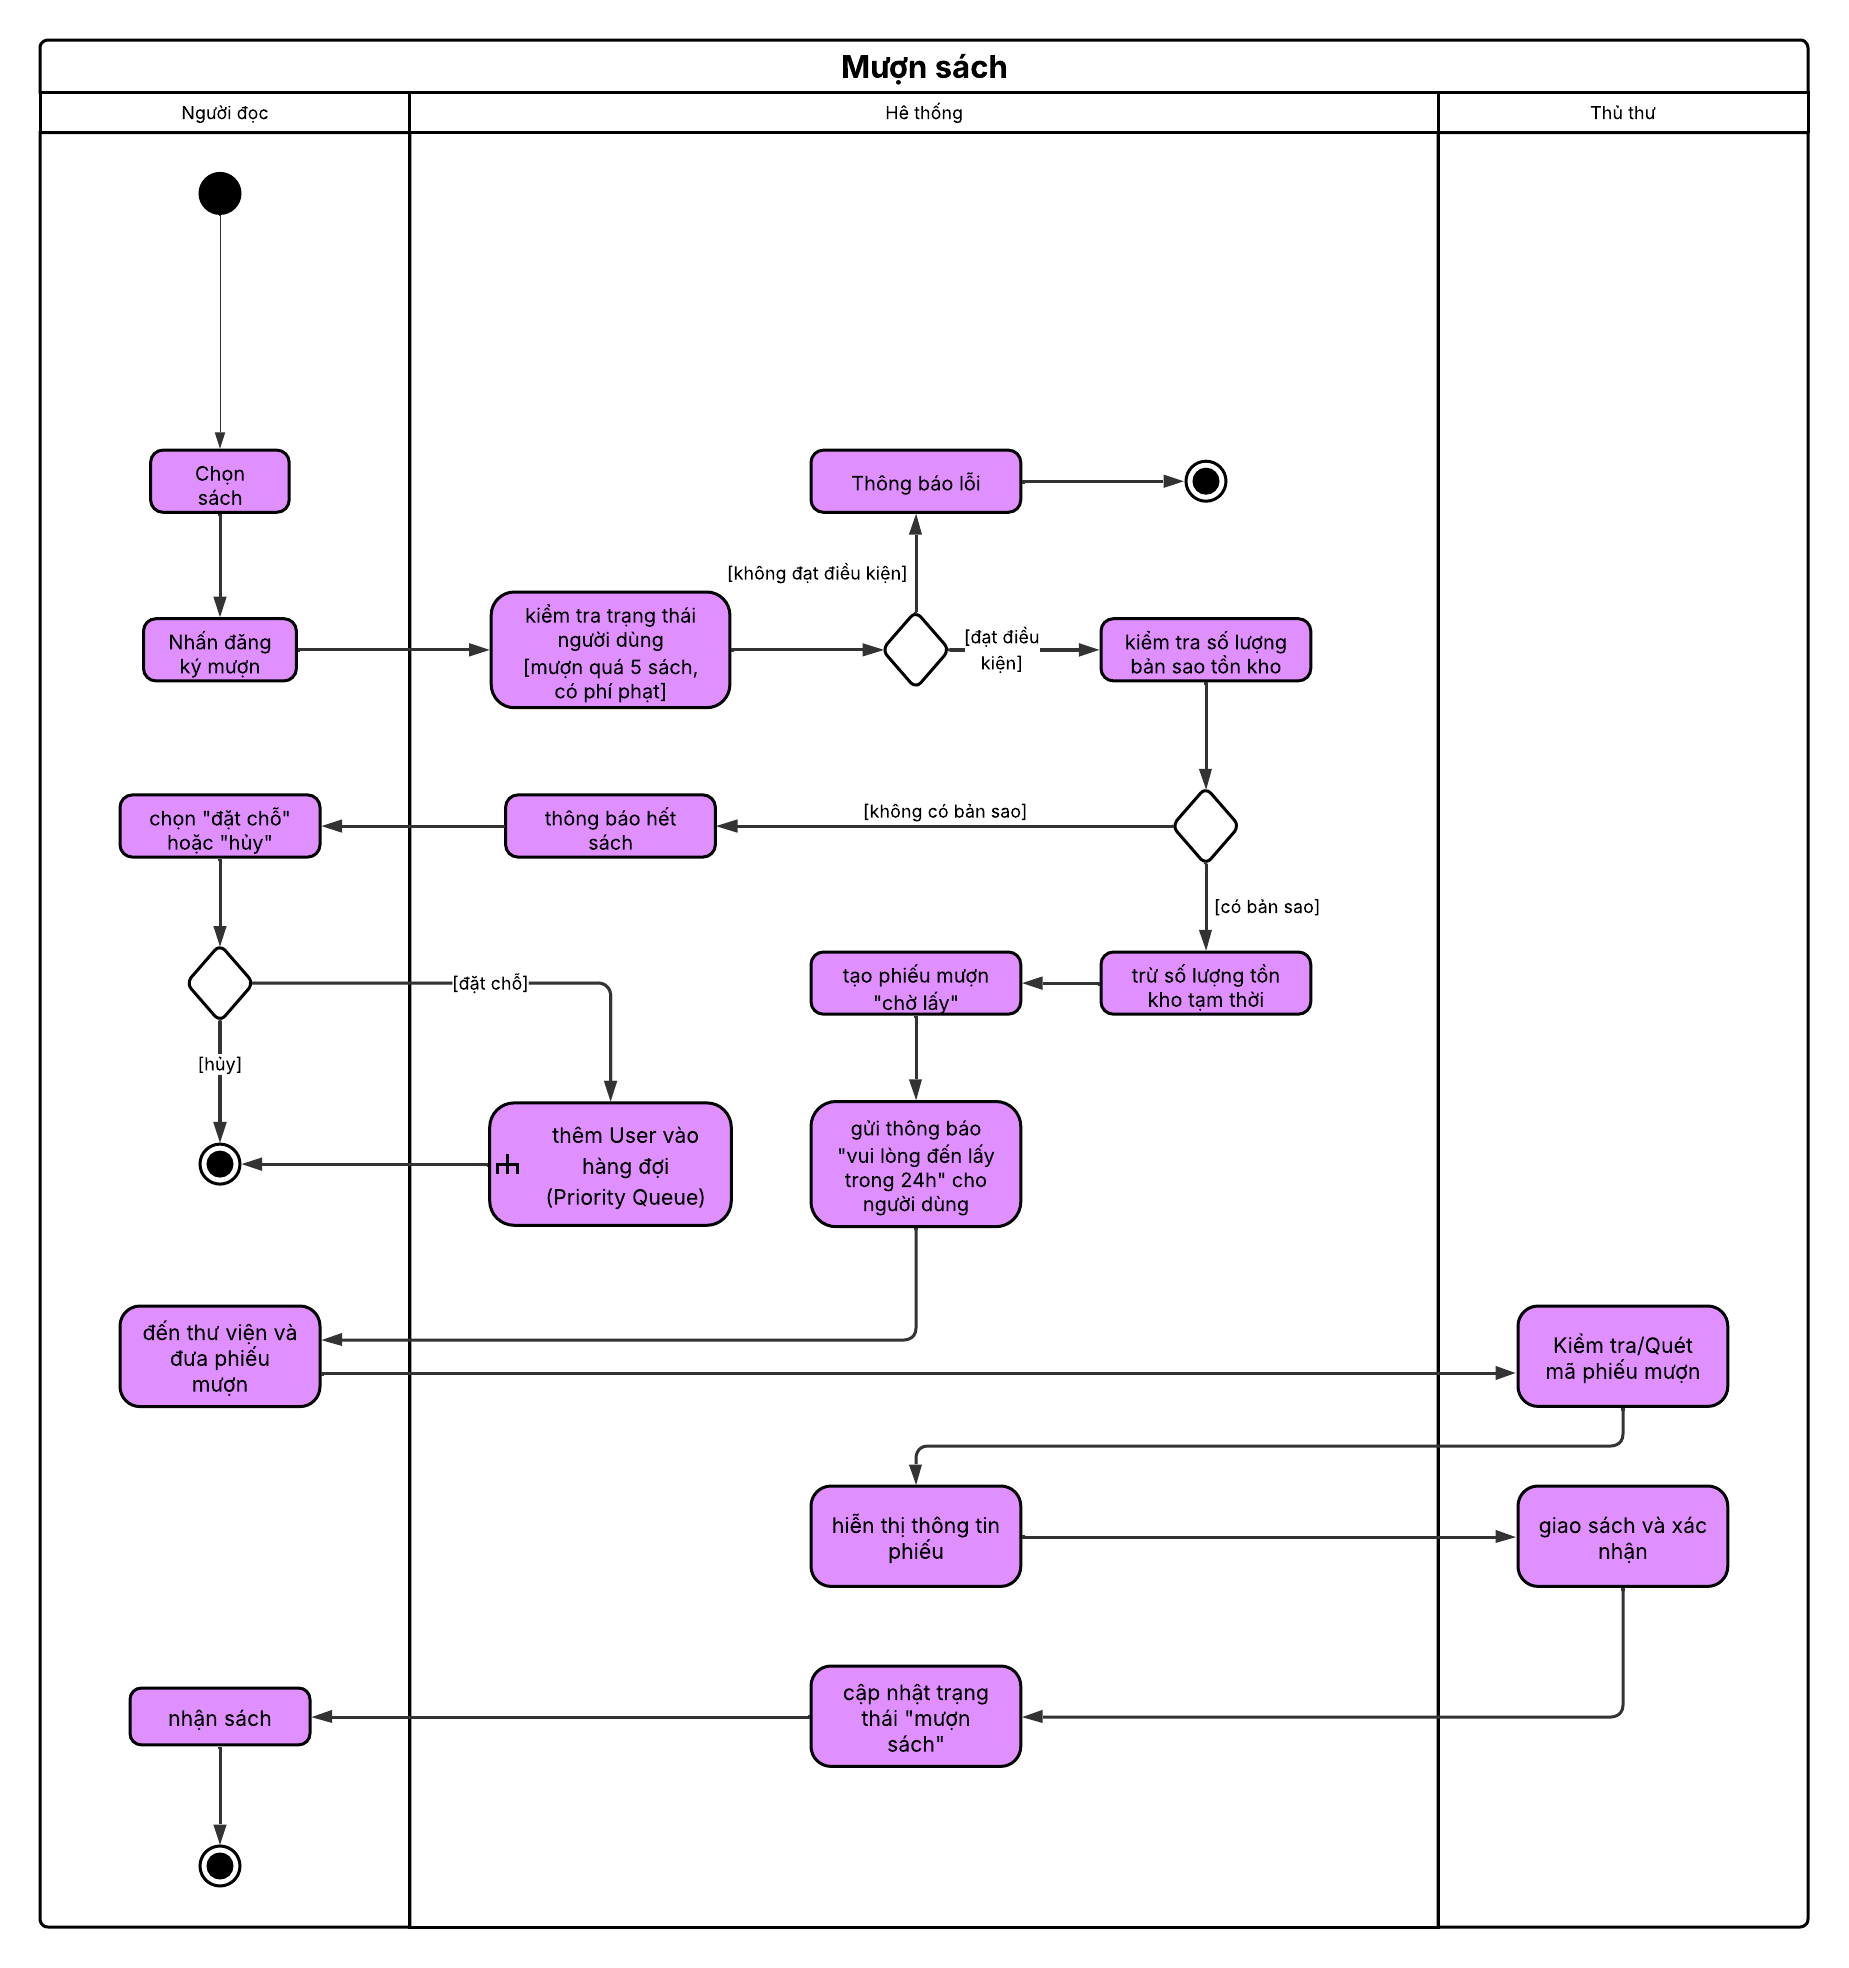
\includegraphics[width=\linewidth]{figures/ch05/activity/borrow_book.png}
 \caption{Mượn sách — Activity Diagram}
 \label{fig:borrow_book}
\end{figure}

\begin{figure}[htbp]
 \centering
 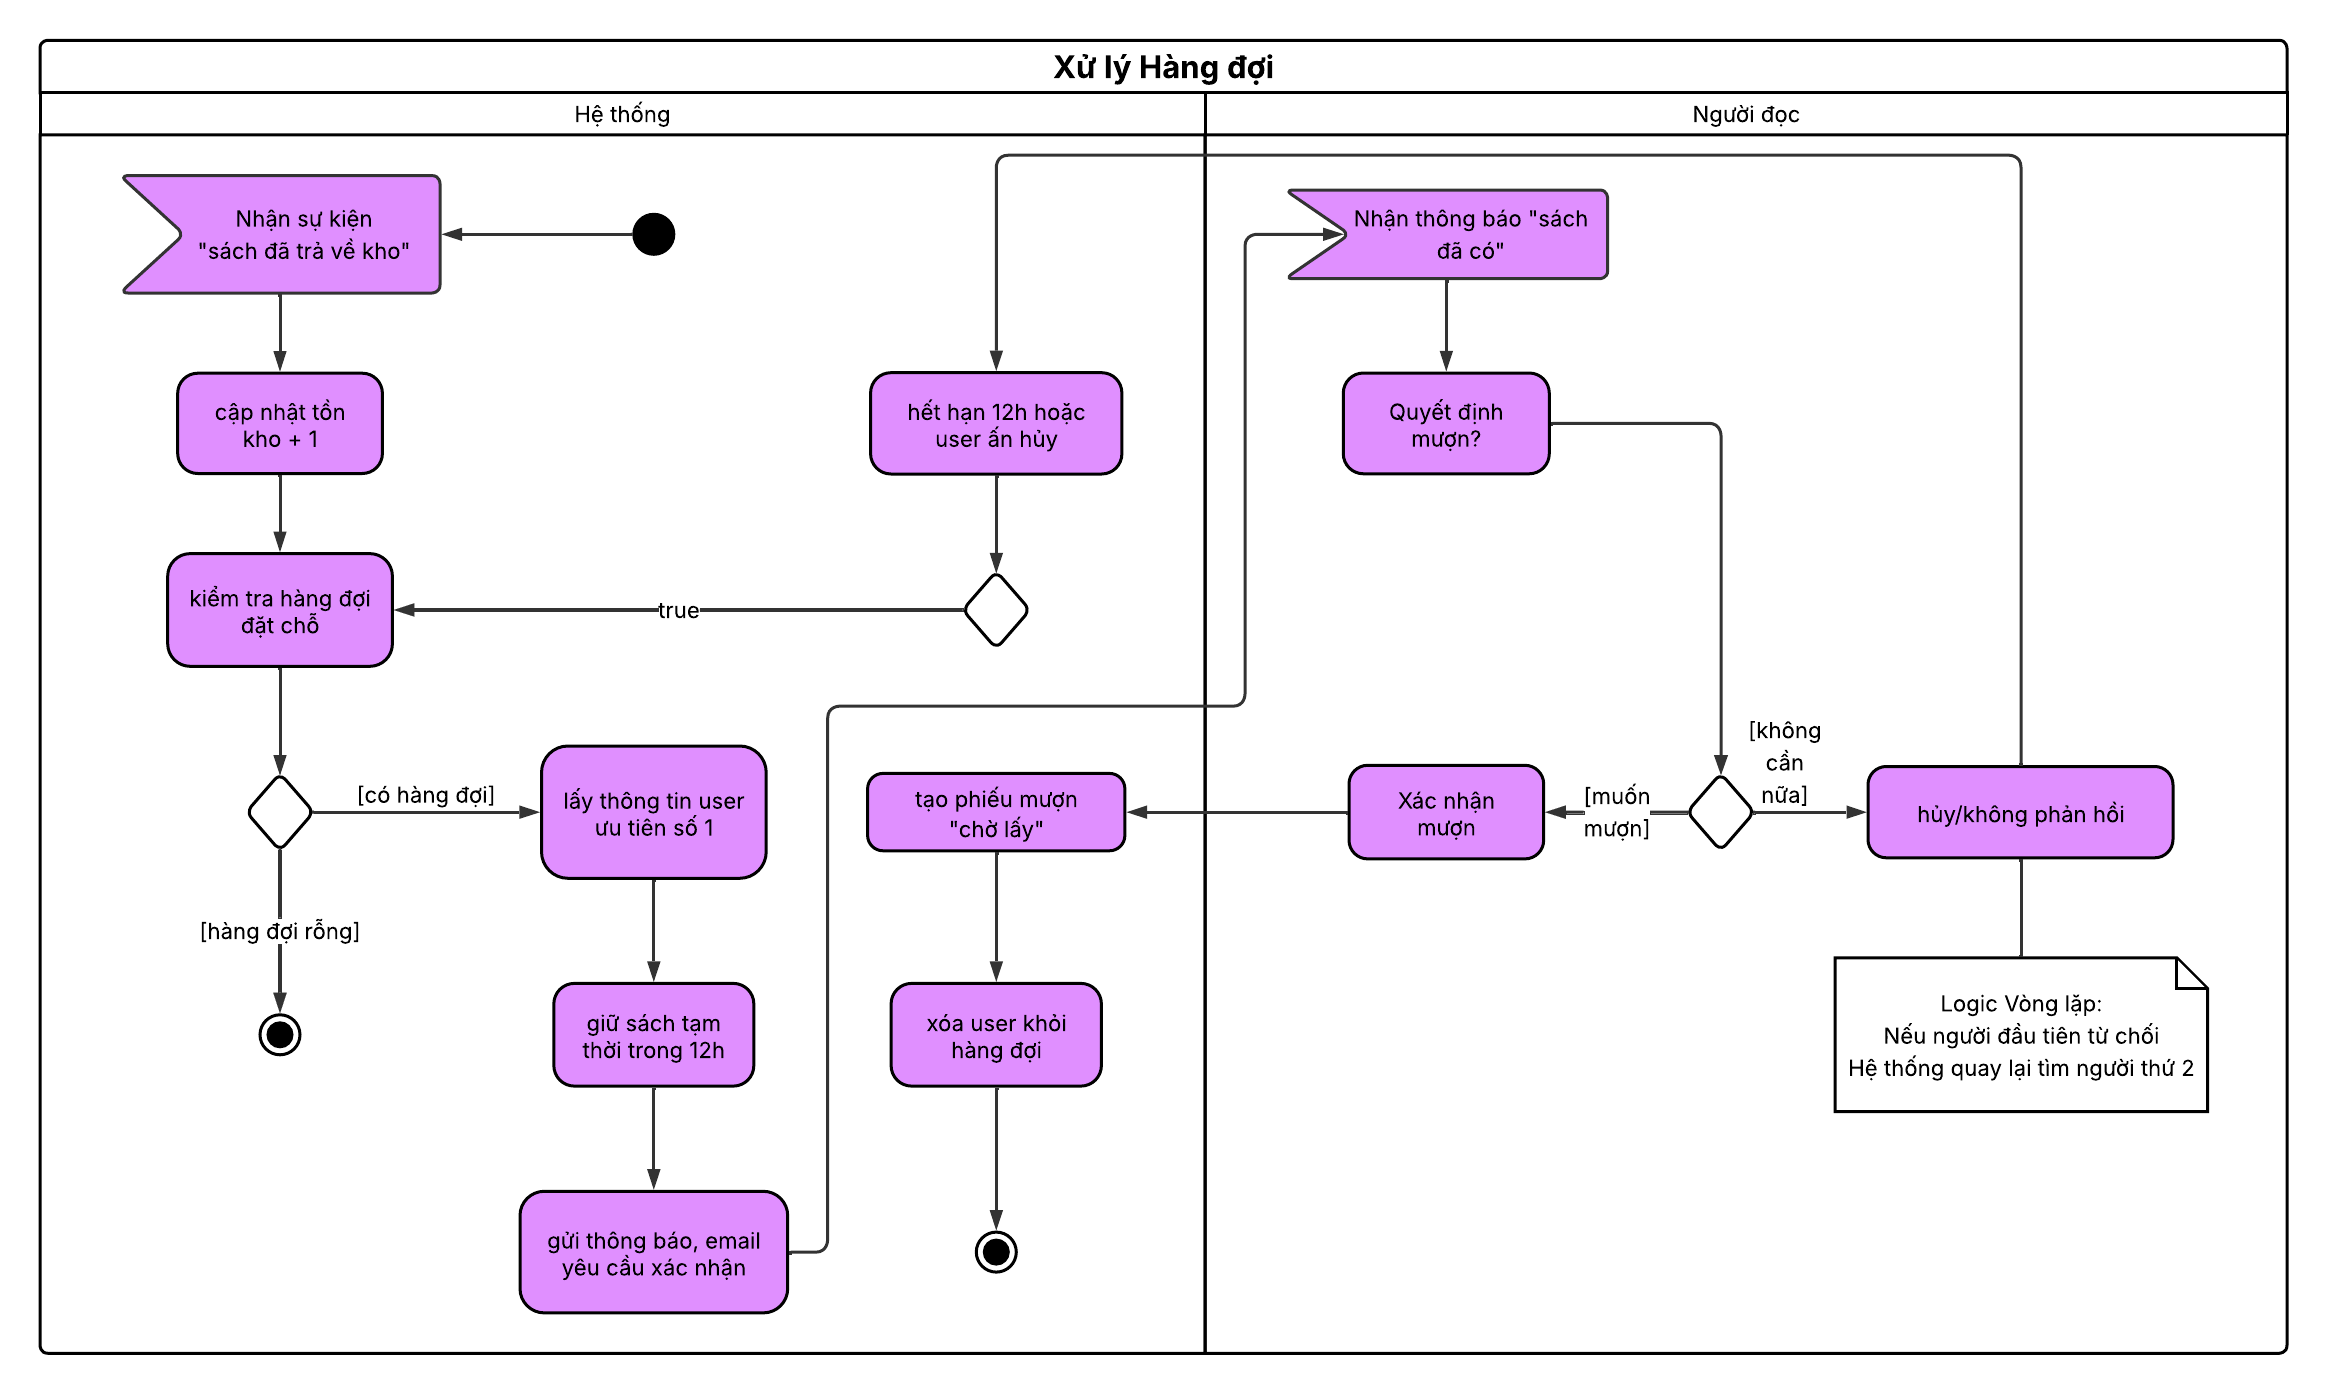
\includegraphics[width=\linewidth]{figures/ch05/activity/process_queue.png}
 \caption{Xử lý hàng đợi đặt trước — Activity Diagram}
 \label{fig:process_queue}
\end{figure}

\begin{figure}[htbp]
 \centering
 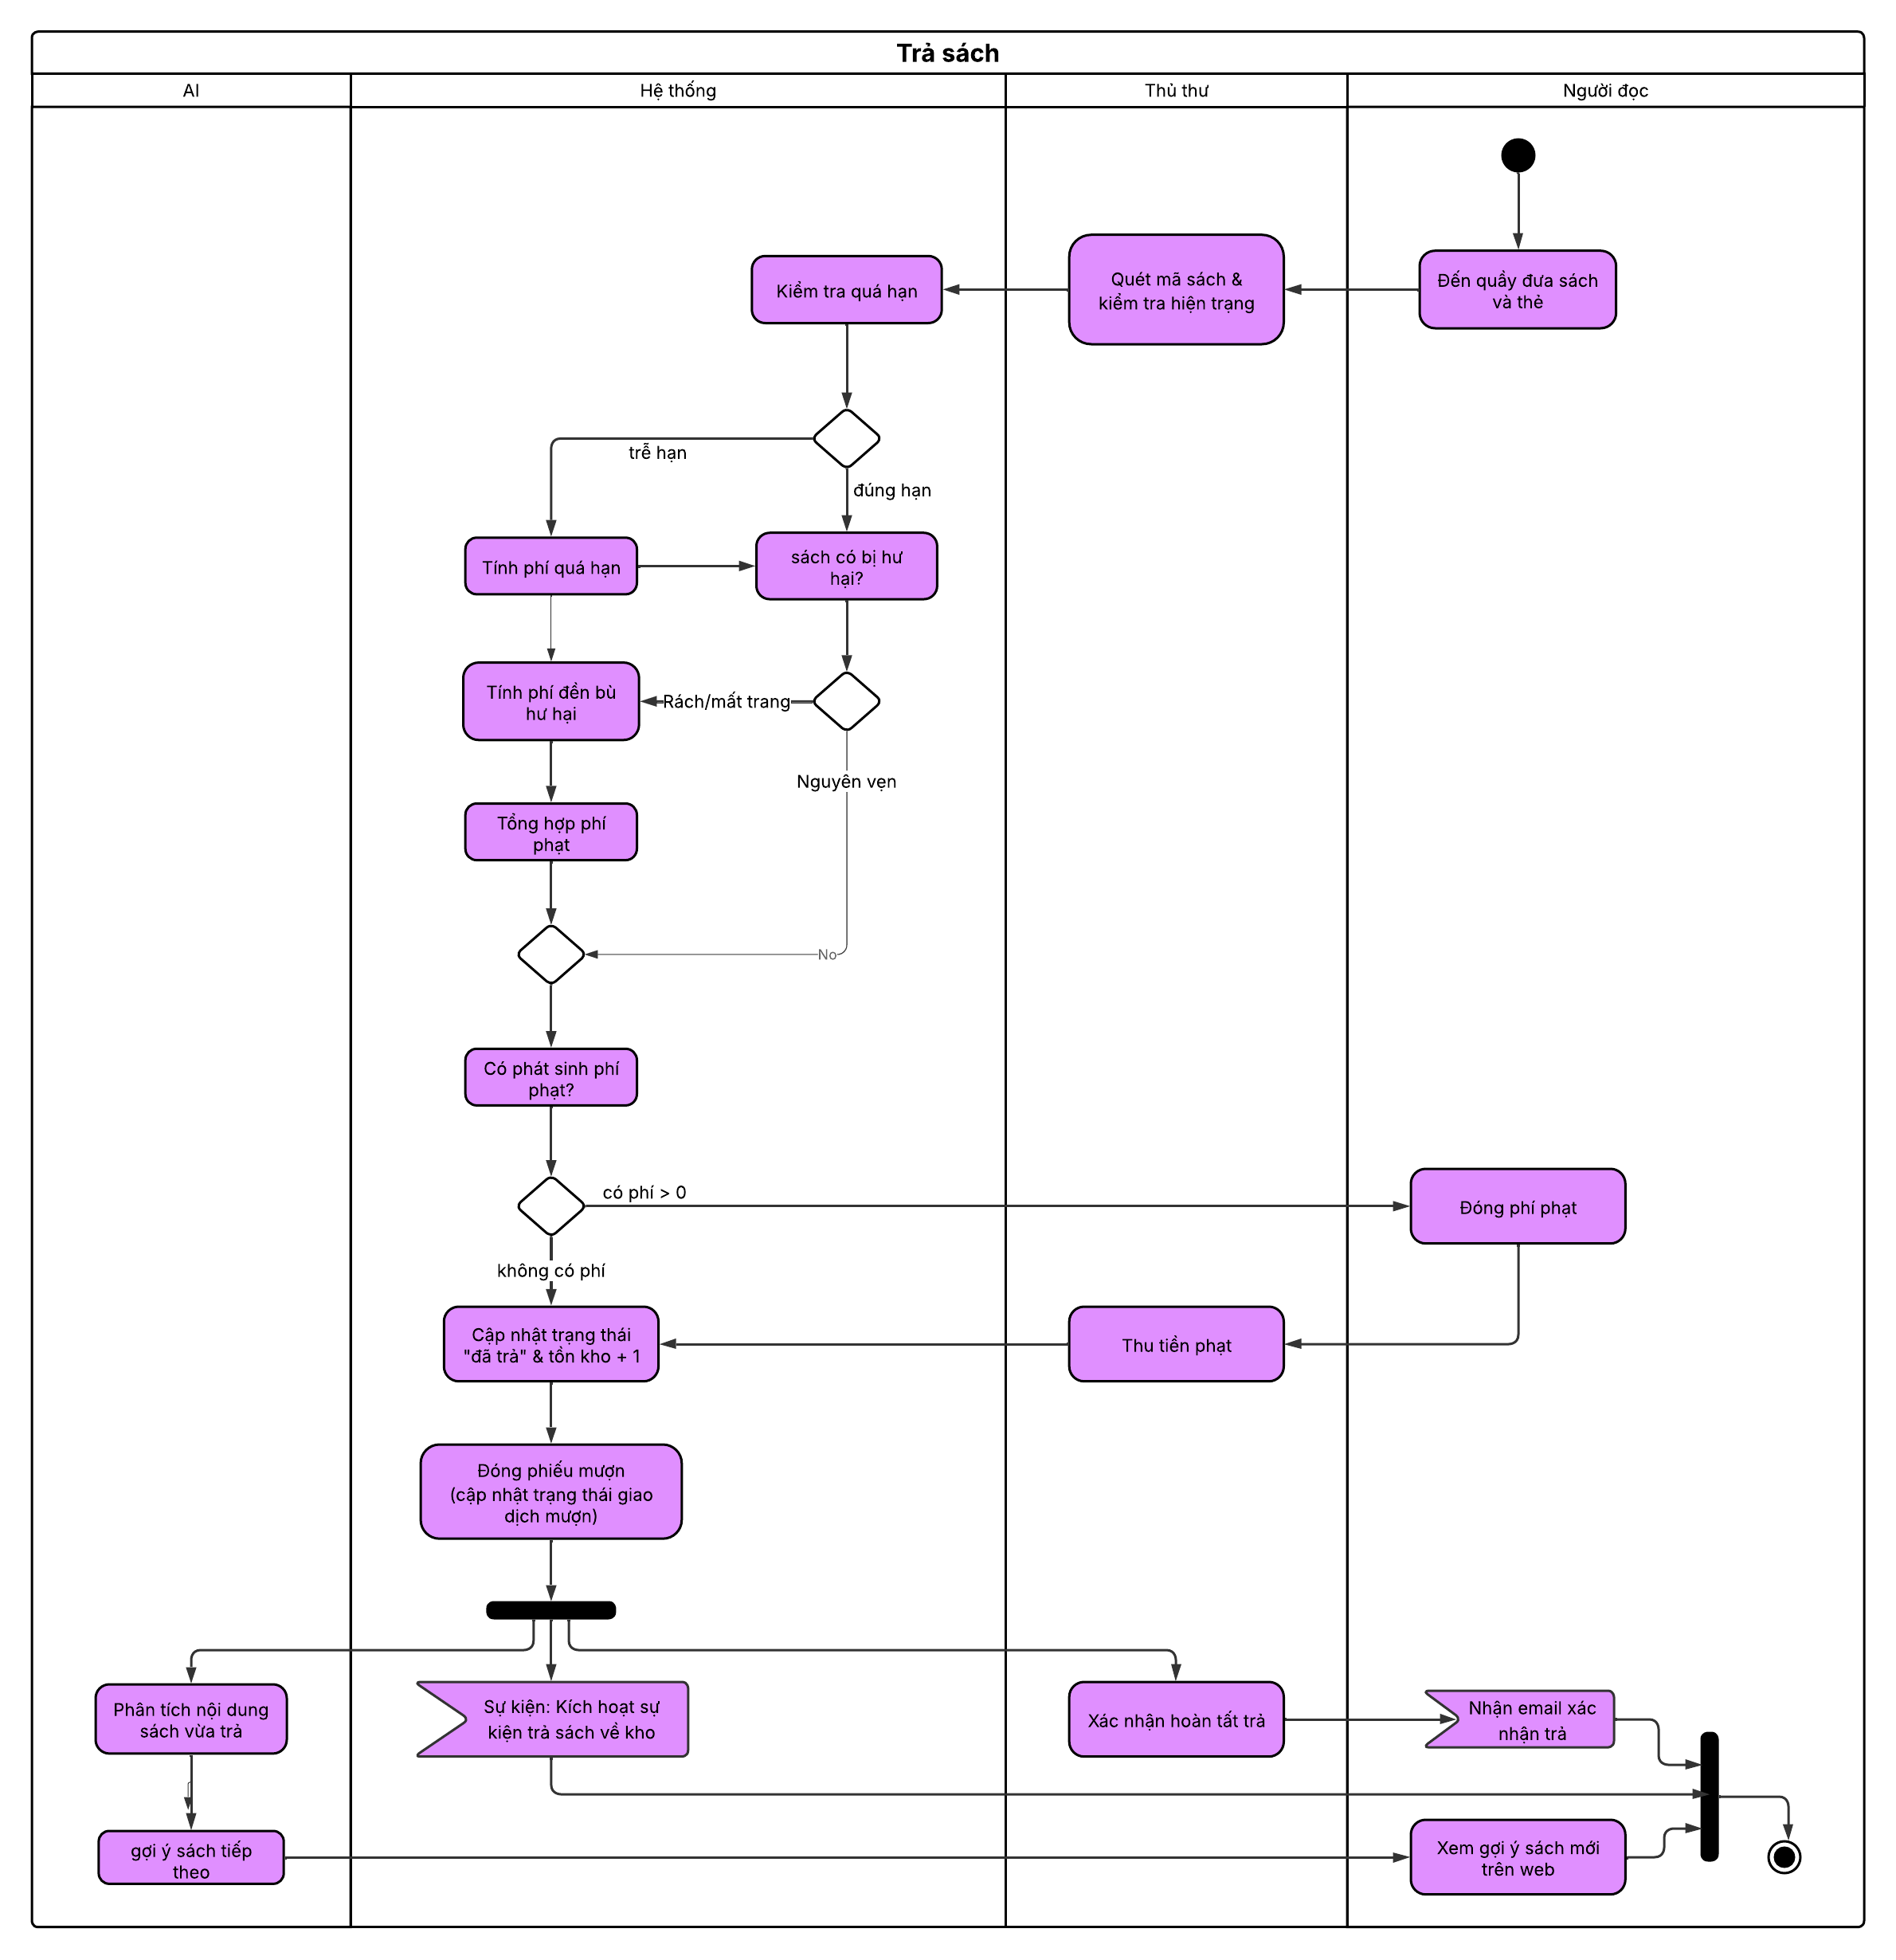
\includegraphics[width=\linewidth]{figures/ch05/activity/return_book.png}
 \caption{Trả sách — Activity Diagram}
 \label{fig:return_book}
\end{figure}

\begin{figure}[htbp]
 \centering
 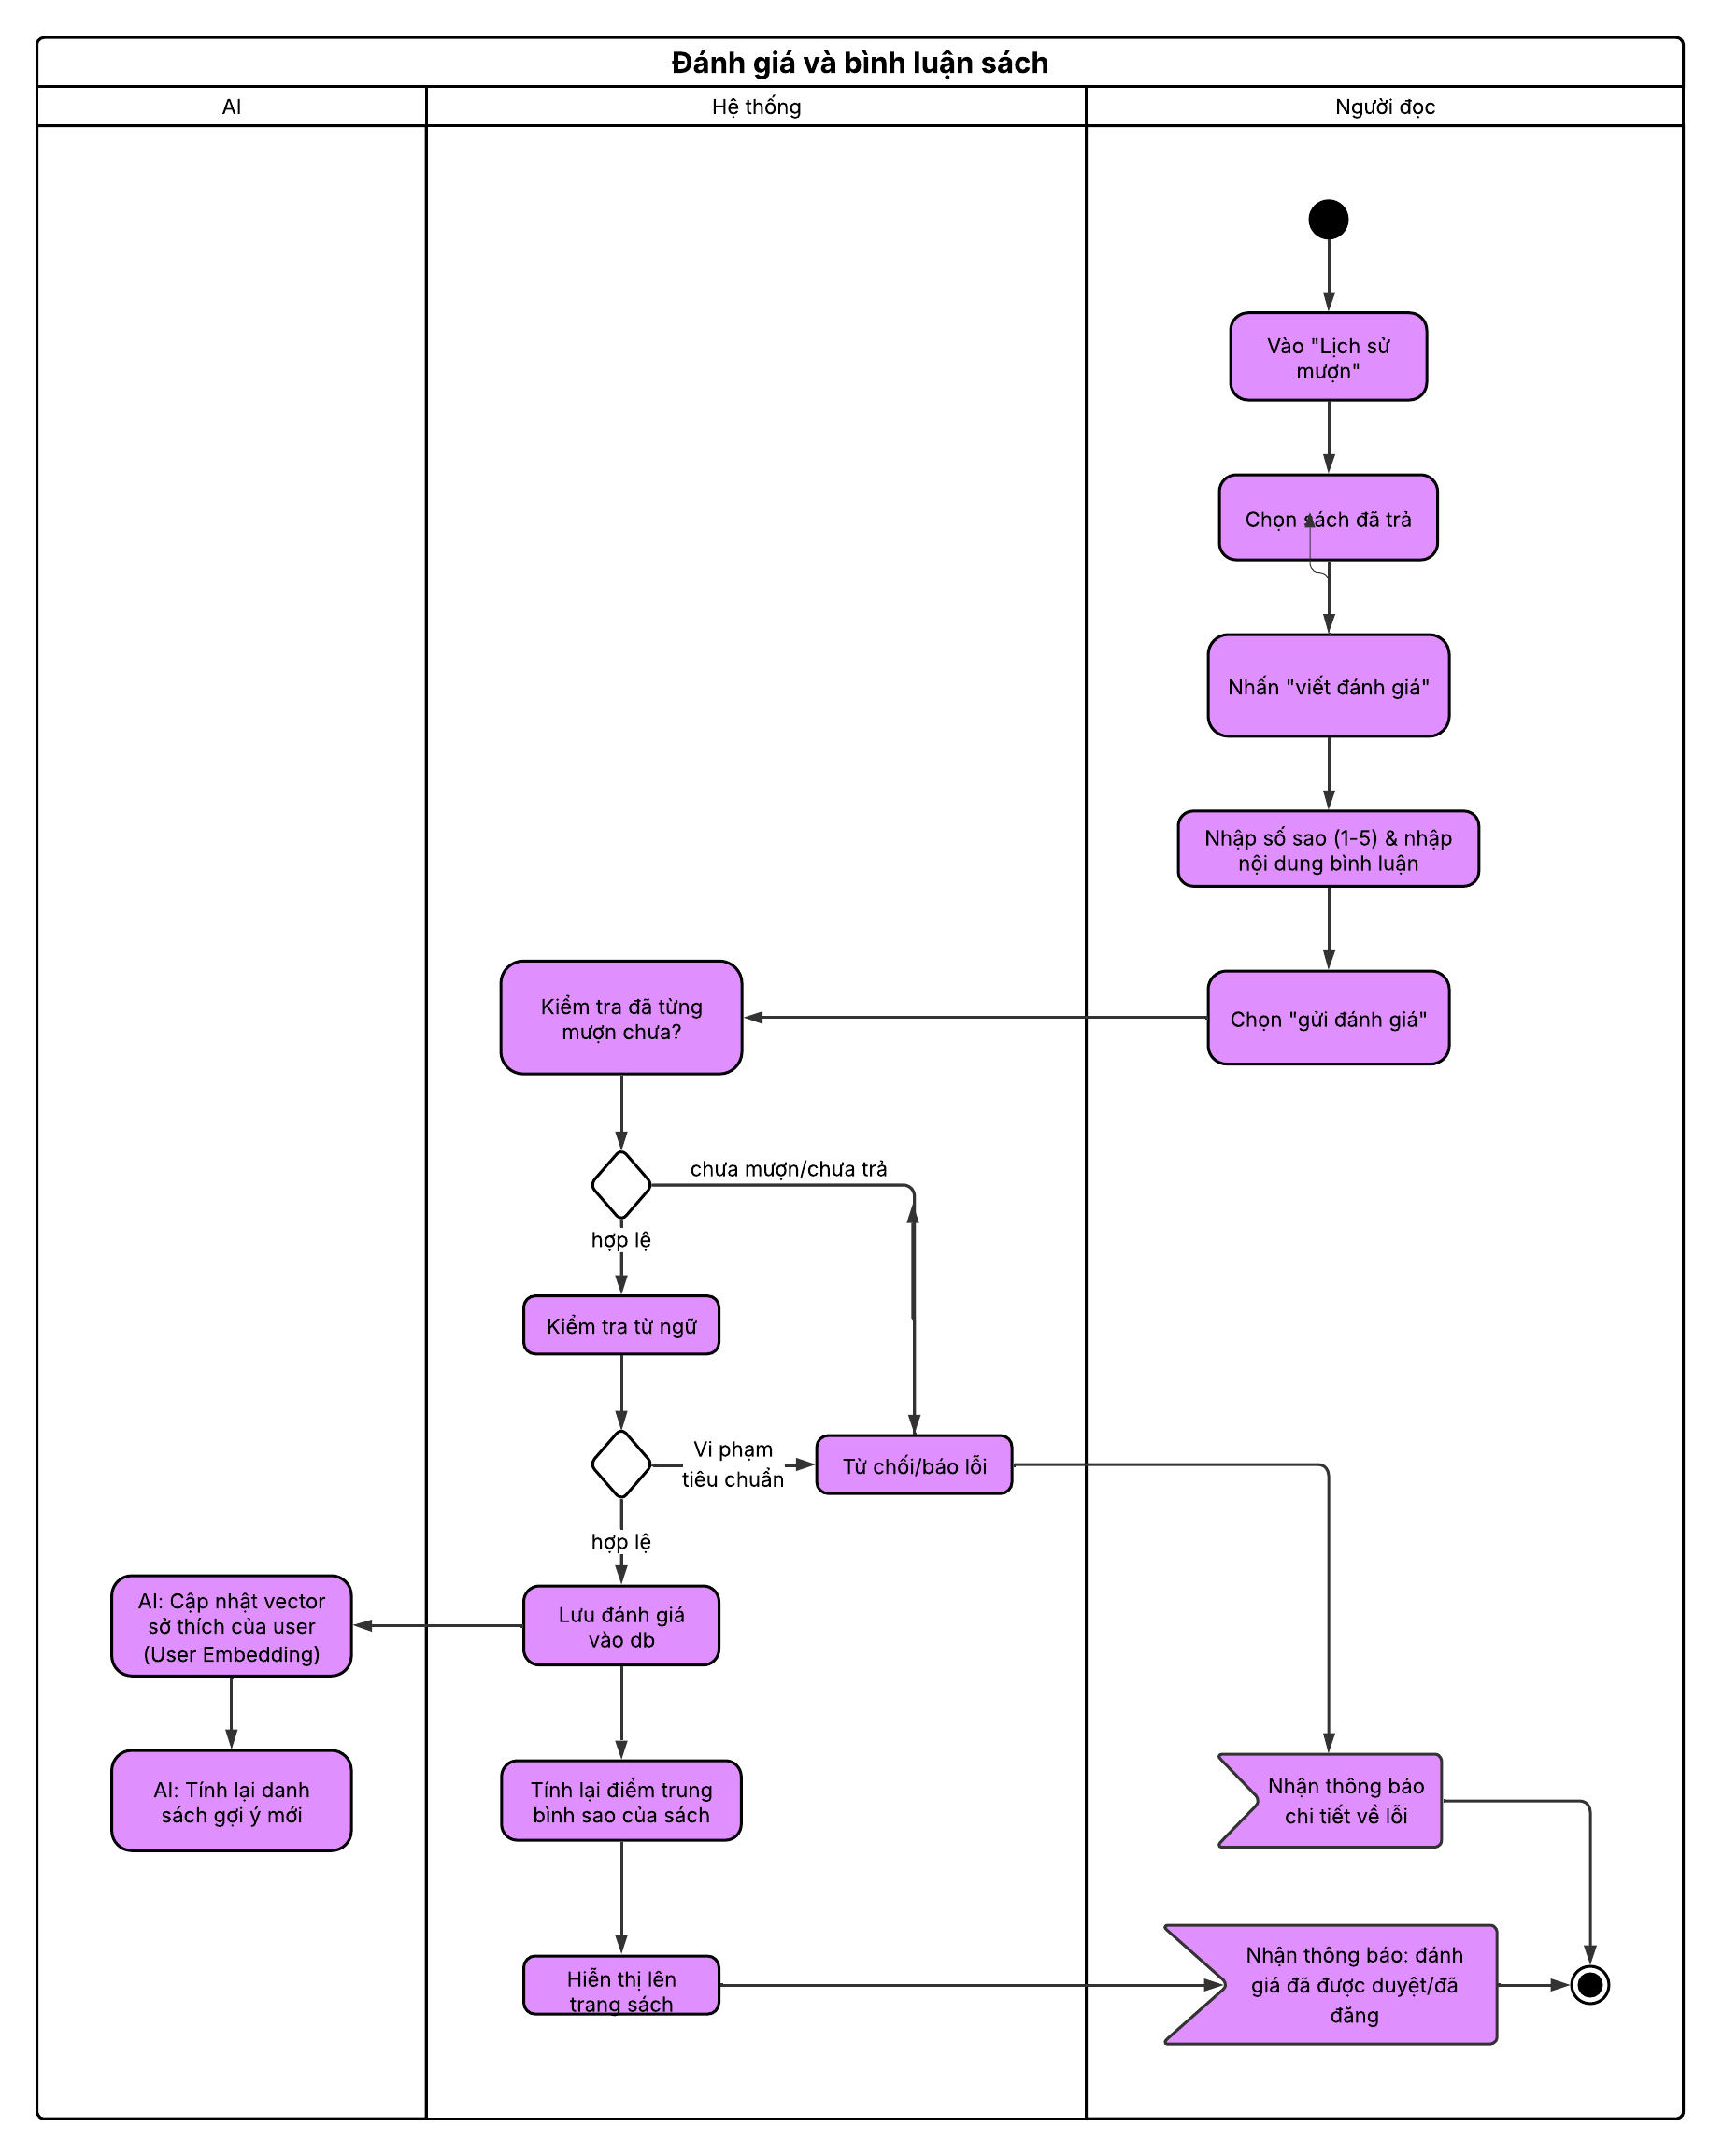
\includegraphics[width=\linewidth]{figures/ch05/activity/review_and_comment.png}
 \caption{Đánh giá và bình luận sách — Activity Diagram}
 \label{fig:book_review_comment}
\end{figure}

\begin{figure}[htbp]
 \centering
 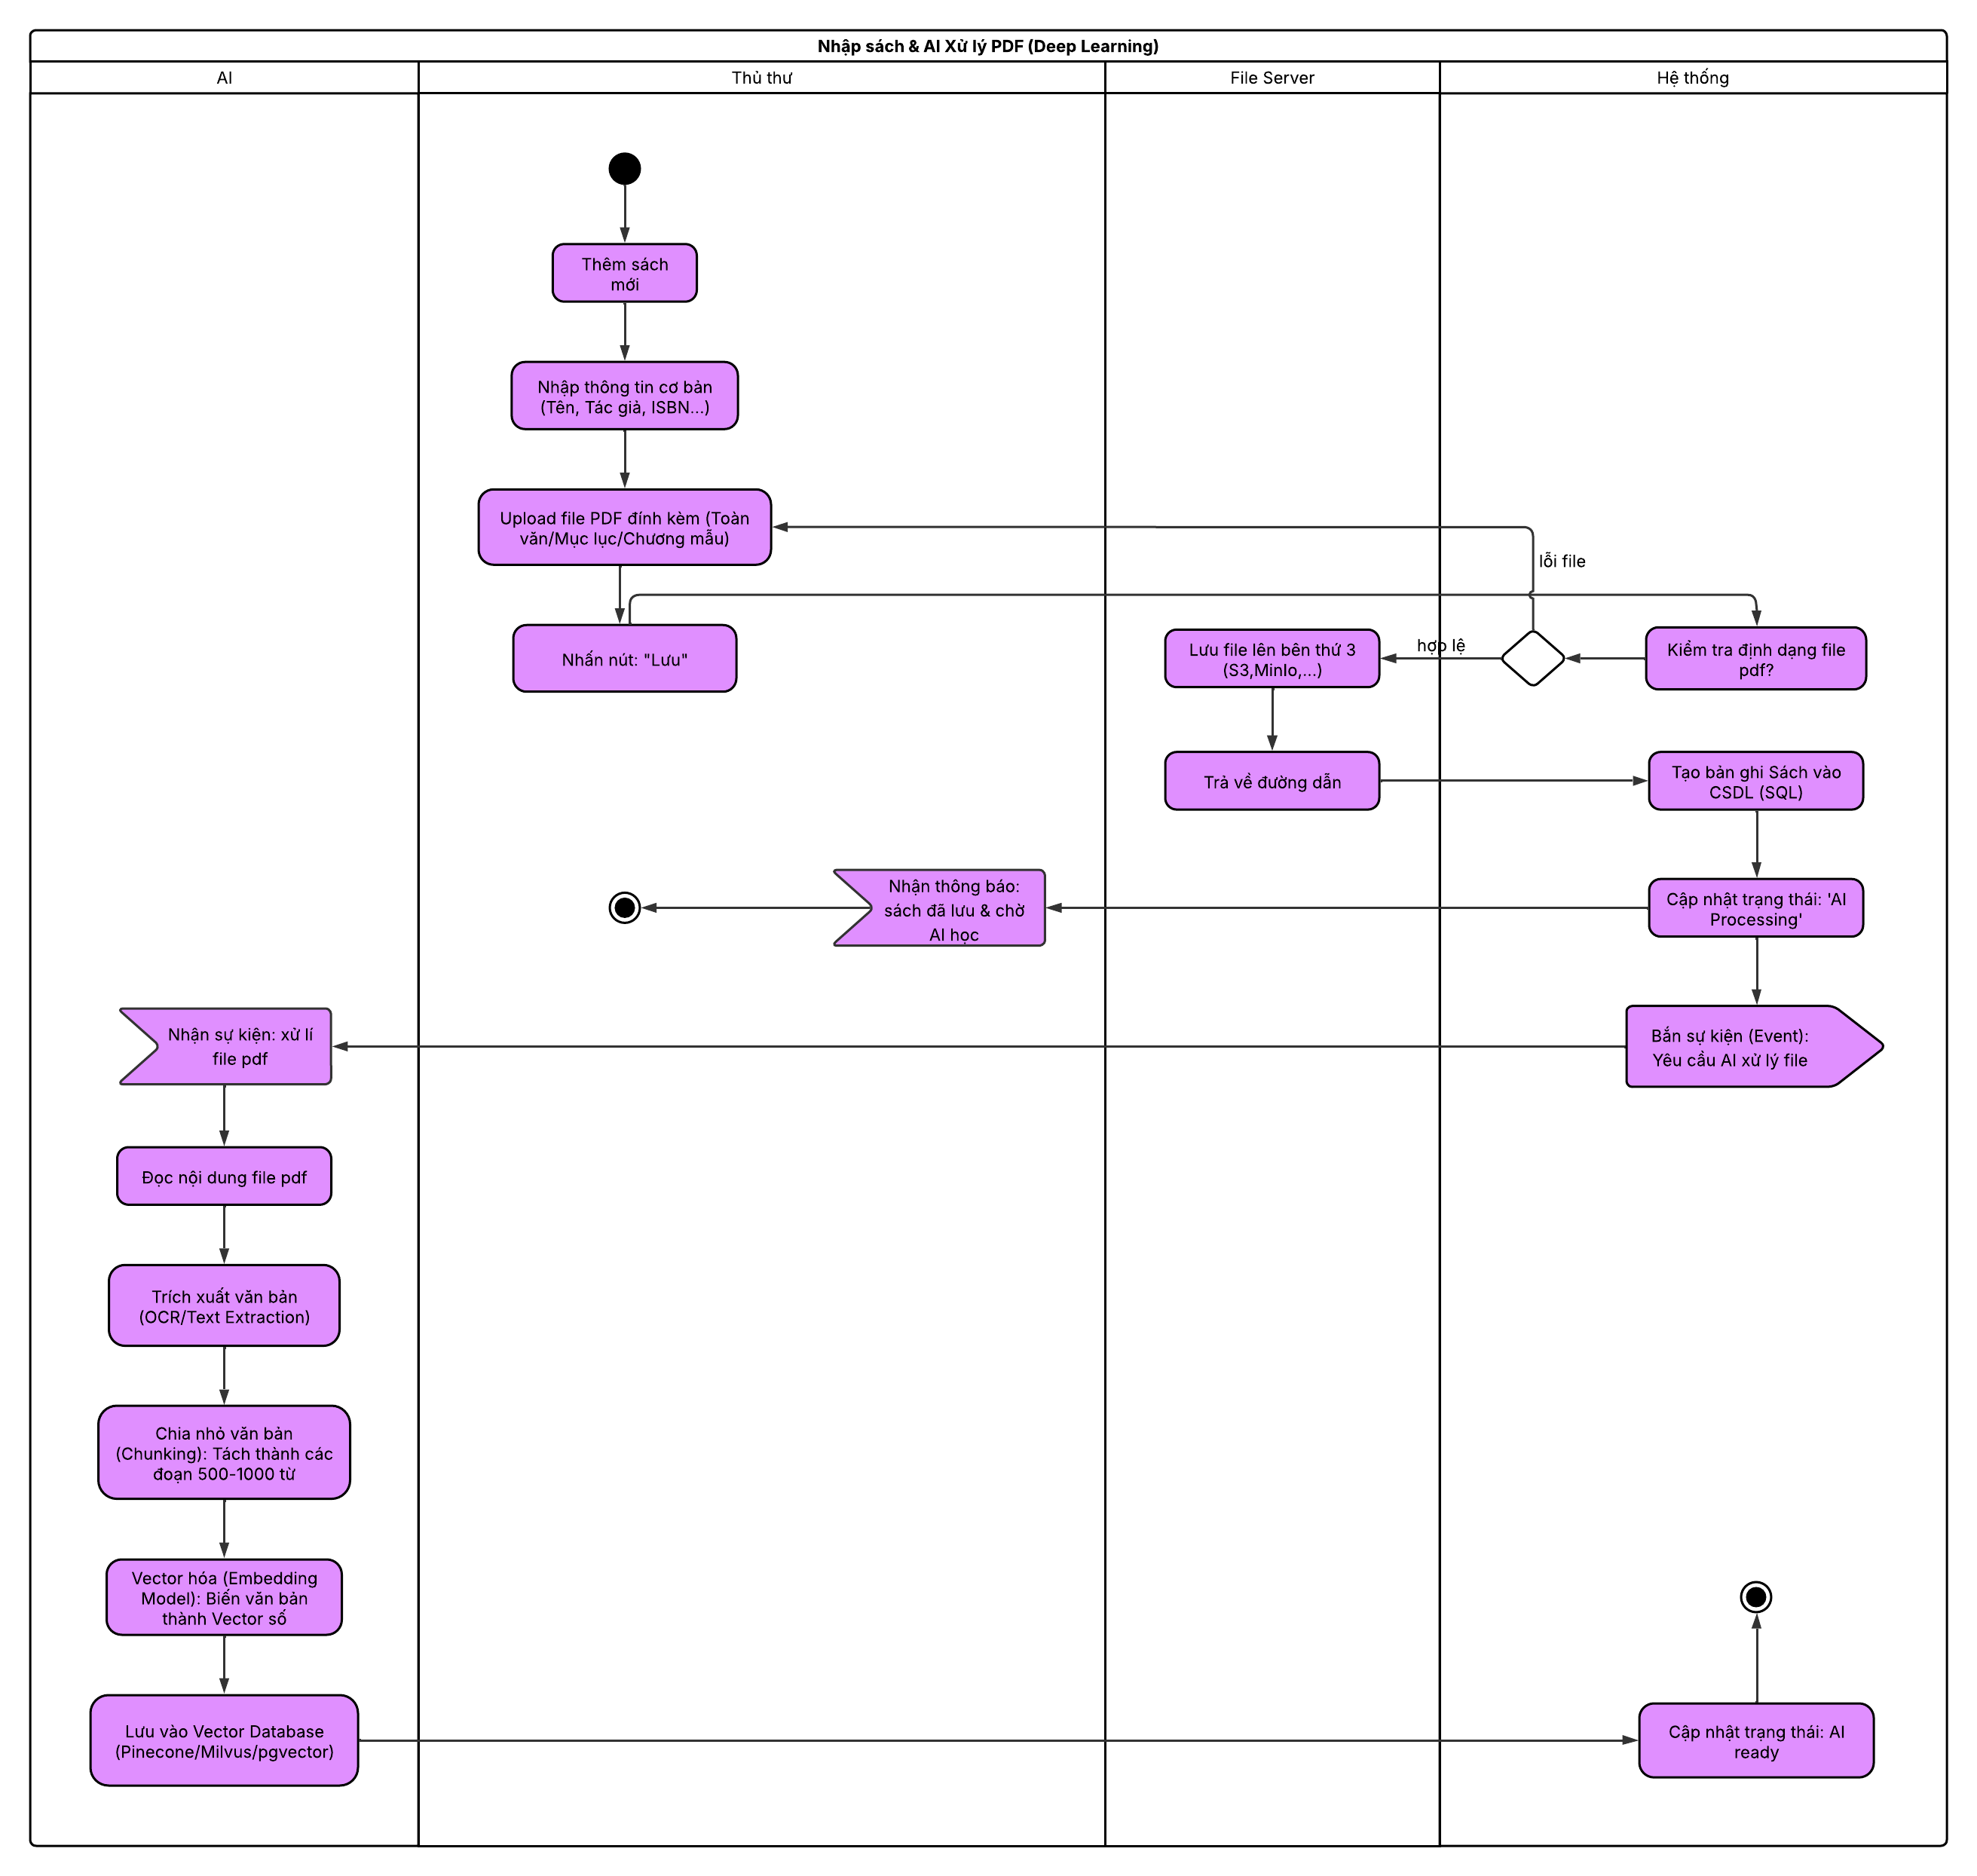
\includegraphics[width=\linewidth]{figures/ch05/activity/add_book.png}
 \caption{Tạo sách với AI — Activity Diagram}
 \label{fig:create_book}
\end{figure}

\FloatBarrier

\section{Giải pháp công nghệ}
\label{sec:giai_phap_cong_nghe}

Việc lựa chọn công nghệ không chỉ dựa trên mức độ phổ biến của framework, mà dựa trên mức độ phù hợp với bài toán thư viện đã hiện thực. Nhóm sử dụng năm tiêu chí chính: \textbf{hiệu năng và độ trễ}, \textbf{khả năng bảo trì}, \textbf{bảo mật và phân quyền}, \textbf{trải nghiệm phát triển}, và \textbf{chi phí triển khai trong phạm vi đồ án}. Từ các tiêu chí này, hệ thống được chia thành ba phần rõ ràng: frontend phục vụ trải nghiệm người dùng, backend giữ nghiệp vụ và dữ liệu giao dịch, còn AI service xử lý các workload tính toán nặng.

\subsection{Front-end}
\label{subsec:frontend_solution}

Frontend của hệ thống là một \textbf{single-page application} phục vụ cả trang public, khu vực bạn đọc và dashboard thủ thư. Đặc điểm chính của phần này là nhiều form nghiệp vụ, nhiều màn hình trạng thái, gọi REST API liên tục, nhận thông báo realtime và upload file PDF trực tiếp lên S3-compatible storage bằng presigned URL. Vì vậy, công nghệ frontend cần nhẹ khi triển khai, dễ chia component và đủ linh hoạt để bám sát thiết kế Figma.

Nhóm đã so sánh các lựa chọn phổ biến theo đúng bối cảnh này:

\begin{table}[H]
\centering
\small
\renewcommand{\arraystretch}{1.12}
\setlength{\tabcolsep}{5pt}
\begin{tabularx}{\linewidth}{|>{\bfseries}l|>{\raggedright\arraybackslash}X|%
>{\raggedright\arraybackslash}X|%
>{\raggedright\arraybackslash}X|}
\hline
\textbf{Nền tảng} & \textbf{Ưu điểm} & \textbf{Nhược điểm} & \textbf{Kết luận} \\
\hline
\textbf{React + Vite} & Phù hợp với SPA nhiều tương tác; build gọn; HMR nhanh; triển khai như static assets; dễ tích hợp REST API, WebSocket/STOMP và presigned upload. Hệ sinh thái React đáp ứng tốt dashboard, form nghiệp vụ và component tái sử dụng. & Không có SSR mặc định; SEO cho public pages không mạnh bằng framework SSR; nhóm phải tự chuẩn hóa routing, state, API layer và cấu trúc component. & \textbf{Được chọn}. Hệ thống chủ yếu là ứng dụng nghiệp vụ sau đăng nhập, không cần SSR phức tạp. React/Vite giúp triển khai đơn giản qua NGINX/Docker, giảm nhu cầu Node runtime và vẫn đủ linh hoạt cho public pages, reader pages và librarian dashboard. \\
\hline
Next.js & Mạnh về SSR/SSG, SEO, route-level data fetching và tối ưu website public lớn. Phù hợp khi nội dung cần index mạnh hoặc cần render phía server. & Cần Node.js runtime, tăng thêm lớp vận hành. Nếu dùng cho hệ thống này, một phần trách nhiệm trình bày và xác thực dễ bị chồng lên Spring Boot API. & Không chọn vì bài toán chính là dashboard và nghiệp vụ thư viện, không phải website nội dung cần SEO mạnh. Lợi ích SSR không đủ bù cho chi phí vận hành thêm. \\
\hline
Nuxt (Vue) & Có SSR/SSG tốt trong hệ sinh thái Vue, cú pháp dễ tiếp cận và tổ chức project rõ ràng. & Không cùng hệ sinh thái với phần frontend đã xây dựng; chuyển sang Vue/Nuxt làm tăng chi phí học lại component, router, test và thư viện UI. & Không chọn vì nhóm đã hiện thực ổn định bằng React và cần tận dụng các thư viện React cho icon, form, realtime notification và dashboard. \\
\hline
Angular & Framework đầy đủ, opinionated, mạnh về form, dependency injection, routing và cấu trúc enterprise. & Boilerplate nhiều, đường cong học tập cao, nặng hơn nhu cầu của nhóm. Việc tùy biến UI nhanh theo Figma kém linh hoạt hơn React trong phạm vi đồ án. & Không chọn vì hệ thống cần tốc độ phát triển và khả năng tinh chỉnh giao diện cao hơn là một framework enterprise lớn ngay từ đầu. \\
\hline
\end{tabularx}
\caption{So sánh công nghệ Front-end theo tiêu chí của hệ thống}
\label{tab:frontend-compare}
\end{table}
\FloatBarrier

\textbf{Lựa chọn:} \emph{React + Vite kết hợp với TypeScript, Tailwind CSS, React Router DOM với HashRouter, Axios, lucide-react, sonner, SockJS/STOMP và một bộ component tự xây dựng theo thiết kế Figma.}

\subsubsection*{Lý do chọn theo tiêu chí chuyên môn}

\begin{itemize}
    \item \textbf{Tốc độ phát triển vượt trội (Developer Experience):}
    Vite tận dụng cơ chế native ES modules trong môi trường phát triển và dùng esbuild cho nhiều bước tiền xử lý, nhờ đó thời gian khởi động dev server và Hot Module Replacement nhanh hơn đáng kể so với cấu hình Webpack truyền thống. Với một frontend có nhiều trang nghiệp vụ, điều này giúp nhóm lặp nhanh khi chỉnh giao diện, form và luồng tương tác.

    \item \textbf{Triển khai đơn giản qua NGINX:}
    React + Vite tạo ra các file tĩnh (HTML/CSS/JS) sau khi build, có thể phục vụ trực tiếp bởi NGINX mà không cần Node.js server runtime. Điều này giúp giảm tài nguyên máy chủ, đơn giản hóa cấu hình Docker và tận dụng khả năng cache tĩnh của NGINX để tăng hiệu năng.

    \item \textbf{Phù hợp với đặc thù hệ thống:}
    Phần lớn giao diện của hệ thống là các trang dashboard và luồng nghiệp vụ dành cho người dùng đã đăng nhập, ví dụ quản lý mượn--trả, đặt trước, phí phạt, thông báo và upload tài liệu. Những trang này ưu tiên tốc độ tương tác và tính ổn định hơn SEO. Bảo mật API được đảm bảo ở Backend Spring Boot bằng JWT và kiểm tra vai trò, nên không cần thêm một lớp server-side rendering trung gian.

    \item \textbf{Hệ sinh thái React và tính nhất quán giao diện:}
    \textbf{TypeScript} giúp giảm lỗi khi tích hợp với API backend, trong khi \textbf{Tailwind CSS}, \textbf{lucide-react}, \textbf{sonner}, \textbf{react-select} và các component tự xây dựng giúp nhóm kiểm soát tốt giao diện mà không phụ thuộc nặng vào một UI framework lớn. Cách làm này phù hợp với hệ thống có nhiều màn hình nghiệp vụ cần tinh chỉnh riêng cho bạn đọc và thủ thư.

    \item \textbf{Quản lý trạng thái và Routing:}
    \textbf{React Router DOM} với \textbf{HashRouter} được dùng để tổ chức các nhóm trang public, reader và librarian, phù hợp với kiểu deploy static qua NGINX. Các trạng thái dùng chung như xác thực, ngôn ngữ, theme, thông báo realtime và upload file được quản lý bằng React Context; các lời gọi API được gom qua Axios service để thống nhất xử lý token, lỗi và phản hồi từ backend.
\end{itemize}

\FloatBarrier

\subsection{Back-end}
\label{subsec:backend_solution}

Backend là phần lõi của hệ thống vì chịu trách nhiệm xác thực, phân quyền, quản lý dữ liệu thư viện và đảm bảo tính nhất quán cho các giao dịch mượn--trả. Khác với frontend, backend không chỉ cần tạo API nhanh mà còn phải xử lý transaction, khóa bản sao khi mượn/trả, phí phạt, đặt trước, webhook thanh toán và callback từ AI service. Vì vậy tiêu chí ưu tiên là độ tin cậy, transaction ACID, bảo mật và khả năng tổ chức module rõ ràng.

\begin{table}[H]
\centering
\small
\renewcommand{\arraystretch}{1.12}
\setlength{\tabcolsep}{5pt}
\begin{tabularx}{\linewidth}{|>{\bfseries}l|>{\raggedright\arraybackslash}X|%
>{\raggedright\arraybackslash}X|%
>{\raggedright\arraybackslash}X|}
 \hline
 \textbf{Nền tảng}
& \textbf{Ưu điểm}
& \textbf{Nhược điểm}
& \textbf{Quyết định} \\
 \hline
 \textbf{Spring Boot}
& Mạnh về nghiệp vụ giao dịch, Spring Security, transaction ACID, JPA/JDBC, validation, scheduler, Kafka/WebSocket và tích hợp dịch vụ ngoài. Phù hợp với mô hình dữ liệu quan hệ chặt chẽ của thư viện.
& Verbose hơn Node/Python; cần thiết kế module rõ ràng để tránh monolith bị rối khi số use case tăng.
& \textbf{Được chọn}. Lõi hệ thống có nhiều nghiệp vụ cần tính nhất quán: mượn--trả, đặt trước, phí phạt, bản sao, thanh toán và phân quyền. Spring Boot giúp kiểm soát transaction, bảo mật và ranh giới module tốt hơn trong bối cảnh hiện thực hiện tại. \\
 \hline
NestJS / Express
& Phát triển API nhanh, TypeScript đồng bộ với frontend, hệ sinh thái lớn và dễ tuyển dụng.
& Express quá tự do nên cần tự chuẩn hóa nhiều thứ; NestJS tốt hơn nhưng transaction, JPA-style domain modeling và security enterprise không tự nhiên bằng Spring Boot trong bài toán này.
& Không được chọn vì lợi thế dùng chung ngôn ngữ không đủ bù cho yêu cầu transaction và phân quyền chặt chẽ của nghiệp vụ thư viện. \\
 \hline
Django / DRF
& CRUD nhanh, admin mạnh, Python thuận lợi nếu gộp chung backend với AI.
& Nếu gộp nghiệp vụ và AI vào một codebase Python, ranh giới giữa transaction nghiệp vụ và workload AI dễ bị lẫn. Khả năng module hóa theo DDD/Clean Architecture trong dự án hiện tại không thuận lợi bằng Spring Boot.
& Không được chọn cho core backend; Python được giữ đúng vai trò ở AI service, nơi hệ sinh thái ML phát huy giá trị nhất. \\
 \hline
MongoDB (NoSQL)
& Schema linh hoạt, dễ lưu tài liệu JSON và mở rộng ngang trong một số bài toán dữ liệu phi cấu trúc.
& Không phù hợp làm datastore chính cho quan hệ nhiều chiều giữa ấn phẩm, bản sao, giao dịch mượn, phí phạt, đặt trước và người dùng. Join, constraint và transaction liên bảng là yêu cầu cốt lõi của hệ thống.
& Không được chọn vì PostgreSQL đáp ứng tốt hơn cả dữ liệu quan hệ lẫn dữ liệu AI nhờ JSONB và pgvector. \\
 \hline
\end{tabularx}
\caption{So sánh công nghệ Back-end theo tiêu chí của hệ thống}
\label{tab:backend-compare}
\end{table}
\FloatBarrier

\textbf{Lựa chọn:} \emph{Spring Boot 3.3, Java 21, Spring Security với JWT/OAuth2, Spring Data JPA kết hợp JDBC Template cho truy vấn đặc thù, PostgreSQL, Flyway, Kafka, WebSocket/STOMP, S3-compatible storage, PayOS và OpenAPI/Swagger. Mô-đun AI/NLP được tách thành một service riêng sử dụng Python/FastAPI.}

\subsubsection*{Lý do chọn theo tiêu chí chuyên môn}
\begin{itemize}
 \item \textbf{Độ tin cậy và Hiệu năng:} Spring Boot là một framework đã được kiểm chứng về độ ổn định và hiệu năng trong các hệ thống enterprise. Kết hợp với \textbf{Java Virtual Machine (JVM)}, nó cung cấp khả năng xử lý đồng thời mạnh mẽ, phù hợp với các tác vụ CRUD và giao dịch phức tạp. Các truy vấn catalog được phân trang và tối ưu bằng PostgreSQL; các tác vụ phụ như email, thông báo và một số xử lý nền được tách khỏi luồng chính bằng Kafka, WebSocket và executor bất đồng bộ.

 \item \textbf{Mô hình Dữ liệu và Khả năng mở rộng:} Nghiệp vụ thư viện có bản chất là quan hệ chặt chẽ. \textbf{Spring Data JPA} và \textbf{Hibernate} cung cấp một tầng ORM (Object-Relational Mapping) mạnh mẽ, cho phép mô hình hóa các thực thể và mối quan hệ phức tạp một cách tự nhiên. Việc sử dụng \textbf{Specification Pattern} giúp xây dựng các truy vấn động một cách an toàn và dễ bảo trì, phục vụ cho các yêu cầu lọc và tìm kiếm phức tạp.

 \item \textbf{Bảo mật Toàn diện:} \textbf{Spring Security} cho phép triển khai xác thực và phân quyền theo vai trò một cách rõ ràng. Hệ thống sử dụng \textbf{JWT} với access token và refresh token cho kiến trúc stateless API; backend chịu trách nhiệm kiểm tra quyền truy cập ở các endpoint quản trị, endpoint mượn--trả, thanh toán và callback từ AI service. Các luồng nhạy cảm như upload file và webhook thanh toán được đặt sau các cơ chế xác thực hoặc chữ ký tương ứng.

 \item \textbf{Ranh giới module rõ ràng:} Backend được tổ chức thành các module Maven như auth, user, catalog, circulation, recommendation và shared. Cách chia này giữ được ưu điểm triển khai đơn giản của modular monolith, nhưng vẫn tạo ranh giới nghiệp vụ đủ rõ để kiểm thử, bảo trì và tách service trong tương lai nếu cần.

 \item \textbf{Dịch vụ AI độc lập:} Việc tách mô-đun AI/NLP thành một service riêng bằng Python/FastAPI là một quyết định kiến trúc có chủ đích. Backend Java giữ phần transaction, phân quyền và nghiệp vụ; AI service giữ phần embedding, semantic search, Gemini reduce và recommendation. Cách chia này tránh nhồi ML workload vào core backend, nhưng vẫn đơn giản hơn việc tách toàn bộ hệ thống thành microservices.
\end{itemize}

\FloatBarrier

\subsection*{Kết luận về Sự phối hợp giữa hai nền tảng}
Kiến trúc tổng thể được thiết kế theo mô hình \textbf{frontend tĩnh + backend API + AI service}. \textbf{React/Vite SPA} chịu trách nhiệm trải nghiệm người dùng và gọi REST API; \textbf{Spring Boot API} giữ vai trò lõi nghiệp vụ, xác thực, phân quyền và điều phối dữ liệu; \textbf{FastAPI AI Service} xử lý các tác vụ nặng như embedding, semantic search và recommendation. Sự phân tách này đủ rõ để bảo trì, nhưng vẫn giữ chi phí triển khai thấp hơn so với một kiến trúc microservices đầy đủ.




\section{Ứng dụng AI vào hệ thống}
% =========================================================================================
Trong hệ thống LMS, AI không được đặt vào như một chức năng phụ để ``làm đẹp'' sản phẩm. AI được thiết kế như một \textbf{lớp năng lực hỗ trợ khám phá tri thức}: đọc nội dung PDF, hiểu ý định tìm kiếm của bạn đọc và đề xuất tài liệu phù hợp với hành vi sử dụng thật.

Điểm quan trọng nhất trong thiết kế là \textbf{AI không thay thế nghiệp vụ thư viện}. Các nghiệp vụ như mượn--trả, đặt trước, quản lý bản sao, phí phạt, thanh toán và phân quyền vẫn do backend Spring Boot kiểm soát. AI Service chỉ xử lý các bài toán phù hợp với ML/NLP, sau đó trả về \textbf{metadata bổ trợ}, \textbf{danh sách \texttt{publication\_id}} hoặc \textbf{chiến lược gợi ý}; backend luôn là nơi lấy dữ liệu cuối cùng trước khi trả về frontend.

\begin{itemize}
    \item \textbf{Module 1 -- Xử lý PDF file:} biến file PDF do thủ thư upload thành dữ liệu có thể tìm kiếm và gợi ý.
    \item \textbf{Module 2 -- Hỗ trợ tìm kiếm ngữ nghĩa:} giúp bạn đọc tìm theo ý định, không chỉ theo từ khóa chính xác.
    \item \textbf{Module 3 -- Gợi ý cá nhân hoá:} kết hợp nội dung sách, hành vi người dùng và fallback nghiệp vụ để đề xuất sách có thể mượn.
\end{itemize}

Nhóm chọn mô hình \textbf{AI Satellite Service}: backend Java giữ nghiệp vụ và giao dịch; AI Service Python/FastAPI xử lý workload nặng như đọc PDF, sinh embedding, truy vấn pgvector và recommendation. Cách tách này giúp hệ thống vừa \textbf{giữ lõi nghiệp vụ ổn định}, vừa \textbf{tận dụng hệ sinh thái AI của Python}.

\begin{figure}[H]
\centering
\begin{tikzpicture}[
    % Sử dụng positioning giúp quản lý khoảng cách các khối linh hoạt và rộng rãi hơn
    node distance=1.5cm and 2.5cm,
    every node/.style={font=\small\sffamily},
    box/.style={rectangle, draw=blue!65!black, fill=blue!5, thick, rounded corners=3pt, minimum width=3.5cm, minimum height=1.2cm, align=center},
    ai/.style={rectangle, draw=green!55!black, fill=green!6, thick, rounded corners=3pt, minimum width=3.5cm, minimum height=1.2cm, align=center},
    db/.style={cylinder, draw=orange!80!black, fill=orange!7, shape border rotate=90, aspect=0.22, minimum width=2.5cm, minimum height=1.5cm, align=center},
    arrow/.style={thick, ->, >=stealth},
    label text/.style={font=\small, midway}
]
    % --- Định nghĩa các khối hệ thống (Nodes) ---
    \node[box] (fe) {Frontend\\React/Vite};
    \node[box, right=of fe] (be) {Backend\\Spring Boot};
    \node[ai, right=of be] (ai) {AI Service\\FastAPI};

    \node[db, below=of be] (pg) {PostgreSQL\\Catalog};
    \node[db, below=of ai] (vec) {pgvector\\AI schema};

    % --- Định nghĩa đường nối luồng dữ liệu (Arrows) ---
    \draw[arrow] (fe) -- node[label text, above] {REST API} (be);
    \draw[arrow] (be) -- node[label text, above] {AI Gateway} (ai);
    \draw[arrow] (be) -- node[label text, left] {nghiệp vụ} (pg);
    \draw[arrow] (ai) -- node[label text, right] {vectors / ETL / cache} (vec);
    \draw[arrow] (vec) -- node[label text, above] {publication ids} (pg);
\end{tikzpicture}
\caption{Trách nhiệm giữa frontend, backend và AI service}
\label{fig:ai_integration_boundary}
\end{figure}

\begin{table}[H]
\centering
\small
\renewcommand{\arraystretch}{1.18}
\setlength{\tabcolsep}{5pt}
\begin{tabularx}{\linewidth}{|>{\bfseries}p{0.23\linewidth}|>{\raggedright\arraybackslash}X|>{\raggedright\arraybackslash}X|}
\hline
\textbf{Thành phần} & \textbf{Trách nhiệm chính} & \textbf{Điểm nhấn thiết kế} \\
\hline
Frontend & Upload tài liệu, gửi truy vấn, hiển thị trạng thái AI và kết quả đã chuẩn hóa. & \textbf{Không gọi trực tiếp model AI}; mọi request đi qua backend. \\
\hline
Backend & Xác thực, phân quyền, lưu catalog, quản lý bản sao/giao dịch và lấy metadata cuối cùng. & \textbf{Là nguồn sự thật nghiệp vụ}; AI không được quyết định trạng thái mượn--trả. \\
\hline
AI Service & Xử lý PDF, sinh embedding, tìm kiếm ngữ nghĩa, tạo metadata AI và recommendation. & \textbf{Chỉ trả kết quả suy luận}; backend quyết định dữ liệu hiển thị cuối cùng. \\
\hline
\end{tabularx}
\caption{Ranh giới trách nhiệm khi tích hợp AI}
\label{tab:ai_responsibility_boundary}
\end{table}

\subsection{Cơ sở thiết kế dữ liệu AI}

Trước khi hiện thực, nhóm xác định rõ AI cần ba nhóm dữ liệu đầu vào. Cách
thiết kế này giúp tránh tình trạng ``có model trước rồi mới tìm dữ liệu'', đồng
thời bảo đảm mỗi thuật toán đều có nguồn tín hiệu khả thi trong hệ thống thư
viện.

\begin{table}[H]
\centering
\small
\renewcommand{\arraystretch}{1.18}
\setlength{\tabcolsep}{4pt}
\begin{tabularx}{\linewidth}{|>{\bfseries}p{0.2\linewidth}|>{\raggedright\arraybackslash}X|>{\raggedright\arraybackslash}X|}
\hline
\textbf{Nhóm dữ liệu} & \textbf{Nguồn trong hệ thống} & \textbf{Dùng cho bài toán AI} \\
\hline
Nội dung tài liệu & PDF, tiêu đề, phụ đề, mô tả, mục lục, tác giả, danh mục, tag. & Embedding, semantic search, sách tương tự, content-based recommendation. \\
\hline
Hành vi người dùng & Lượt xem, wishlist, mượn sách, rating, lịch sử tìm kiếm. & Collaborative filtering, ALS implicit feedback, trending fallback. \\
\hline
Trạng thái nghiệp vụ & Sách còn bản sao hay không, chi nhánh, trạng thái bản sao, quyền truy cập. & Lọc kết quả cuối cùng để gợi ý/tìm kiếm có giá trị sử dụng thật. \\
\hline
\end{tabularx}
\caption{Nguồn dữ liệu dùng cho thiết kế AI}
\label{tab:ai_data_sources_design}
\end{table}

Về mặt lưu trữ, nhóm chọn hướng \textbf{vector theo chunk} thay vì một vector
duy nhất cho cả sách. Một sách có thể bao gồm nhiều chủ đề; nếu chỉ dùng một
vector trung bình cho toàn bộ tài liệu, các chương nhỏ nhưng quan trọng dễ bị
loãng. Vì vậy, mỗi chunk có một embedding riêng và liên kết về
\texttt{publication\_id}.

\begin{lstlisting}[language=SQL, caption={Thiết kế bảng vector phục vụ semantic search}, label={lst:ai_vector_schema_design}]
CREATE TABLE ai_engine.publication_vectors (
    id BIGSERIAL PRIMARY KEY,
    publication_id BIGINT NOT NULL,
    chunk_index INT NOT NULL,
    chunk_text TEXT NOT NULL,
    embedding VECTOR(768) NOT NULL,
    created_at TIMESTAMP DEFAULT NOW()
);

CREATE INDEX idx_publication_vectors_embedding
ON ai_engine.publication_vectors
USING hnsw (embedding vector_cosine_ops);
\end{lstlisting}

\FloatBarrier

\subsection{Module 1: Xử lý PDF file}

\textbf{Mục tiêu của module này} là biến một file PDF thô thành dữ liệu có giá trị cho hệ thống: \textbf{summary}, \textbf{audience}, \textbf{tag}, \textbf{vector embedding} và \textbf{trạng thái xử lý AI}. Đây là module nền tảng: nếu PDF không được xử lý tốt, semantic search và recommendation phía sau sẽ không có đủ dữ liệu để hoạt động.

Luồng xử lý được thiết kế theo hướng \textbf{không chặn thao tác của thủ thư}. Thủ thư chỉ cần upload tài liệu; backend lưu URL tài liệu và kích hoạt AI xử lý ở phía sau.

\begin{figure}[H]
\centering
\resizebox{\linewidth}{!}{%
\begin{tikzpicture}[
    every node/.style={font=\small},
    flowstep/.style={rectangle, draw=blue!70!black, fill=blue!5, thick, rounded corners, minimum width=3.05cm, minimum height=1.0cm, align=center},
    store/.style={cylinder, draw=orange!80!black, fill=orange!8, shape border rotate=90, aspect=0.25, minimum width=2.3cm, minimum height=1.35cm, align=center},
    resultnode/.style={rectangle, draw=green!55!black, fill=green!6, thick, rounded corners, minimum width=3.2cm, minimum height=1.0cm, align=center},
    arrow/.style={thick, ->, >=stealth}
]
    \node[flowstep] (fe) at (0,0) {1. Thủ thư\\chọn PDF};
    \node[flowstep] (url) at (3.8,0) {2. Backend cấp\\upload URL};
    \node[store] (s3) at (7.2,0) {Object\\Storage};
    \node[flowstep] (save) at (10.8,0) {3. Lưu\\\texttt{file\_url}};
    \node[resultnode] (ai) at (10.8,-2.0) {4. Gọi AI\\process PDF};
    \node[resultnode] (etl) at (7.2,-2.0) {5. Clean\\chunk\\embed};
    \node[resultnode] (meta) at (3.8,-2.0) {6. Gemini\\reduce metadata};
    \node[store] (db) at (0,-2.0) {DB\\AI outputs};

    \draw[arrow] (fe) -- (url);
    \draw[arrow] (url) -- (s3);
    \draw[arrow] (s3) -- (save);
    \draw[arrow] (save) -- (ai);
    \draw[arrow] (ai) -- (etl);
    \draw[arrow] (etl) -- (meta);
    \draw[arrow] (meta) -- (db);
\end{tikzpicture}
}
\caption{Module 1 -- Luồng xử lý PDF file sau khi thủ thư upload}
\label{fig:ai_pdf_processing_flow}
\end{figure}

\begin{table}[H]
\centering
\small
\renewcommand{\arraystretch}{1.15}
\setlength{\tabcolsep}{4pt}
\begin{tabularx}{\linewidth}{|>{\bfseries}p{0.22\linewidth}|>{\raggedright\arraybackslash}X|>{\raggedright\arraybackslash}X|}
\hline
\textbf{Giai đoạn} & \textbf{Thiết kế} & \textbf{Điểm nhấn báo cáo} \\
\hline
Upload và lưu file & Frontend xin \textbf{presigned upload URL}; file PDF được đẩy lên object storage; backend lưu lại \texttt{file\_url}/\texttt{s3Key} cho publication. & \textbf{File được lưu trước, AI xử lý sau}; thao tác tạo/cập nhật sách không bị khóa bởi pipeline AI. \\
\hline
ETL nội dung & AI Service dùng \textbf{PyMuPDF} để trích xuất text, làm sạch header/footer/số trang, sau đó chia chunk bằng sliding window. & \textbf{Index nội dung thật của PDF}, không chỉ index tiêu đề hay mô tả thủ công. \\
\hline
Embedding và metadata & Chunk được vector hóa và lưu vào \texttt{ai\_engine.publication\_vectors}; Gemini chỉ được gọi ở bước reduce để tạo summary, audience và tag. & \textbf{Không gọi LLM trong mỗi lần tìm kiếm}; giảm độ trễ, giảm quota và tăng độ ổn định. \\
\hline
Theo dõi trạng thái & Kết quả xử lý được lưu với trạng thái \texttt{RUNNING}, \texttt{SUCCESS}, \texttt{FAILED}; nếu lỗi, catalog vẫn giữ ấn phẩm. & \textbf{AI lỗi không làm hỏng nghiệp vụ thư viện}. \\
\hline
\end{tabularx}
\caption{Thiết kế Module 1 -- Xử lý PDF file}
\label{tab:ai_module_pdf}
\end{table}

\subsubsection{Thiết kế chunking, embedding và reduce metadata}

PDF không được đưa thẳng vào LLM. Nhóm thiết kế pipeline theo hướng
\textbf{extract trước, chunk sau, embedding độc lập, LLM chỉ reduce}. Cách này
giảm chi phí gọi LLM và làm cho semantic search có thể chạy hoàn toàn trên
vector đã tính sẵn.

\begin{table}[H]
\centering
\small
\renewcommand{\arraystretch}{1.18}
\begin{tabularx}{\linewidth}{|>{\bfseries}p{0.22\linewidth}|>{\raggedright\arraybackslash}X|>{\raggedright\arraybackslash}X|}
\hline
\textbf{Bước} & \textbf{Thiết kế trước hiện thực} & \textbf{Lý do} \\
\hline
Làm sạch PDF & Bỏ header/footer lặp, số trang, ký tự null, khoảng trắng nhiễu và từ bị ngắt dòng. & Vector phải biểu diễn nội dung thật, không học nhiễu trình bày. \\
\hline
Sliding window chunk & Chia text thành các đoạn độ dài $L$, overlap $O$, bước nhảy $S=L-O$. & Giữ ngữ cảnh giữa hai chunk liền kề, tránh cắt mất câu/ý. \\
\hline
Normalize embedding & Với chunk $c_i$, tính $e_i=\frac{f(c_i)}{\|f(c_i)\|_2}$. & Vector đã chuẩn hóa giúp cosine similarity ổn định. \\
\hline
Chọn chunk đại diện & Ưu tiên chunk mở đầu, chunk gần centroid và chunk đa dạng theo MMR. & Reduce metadata cần đại diện toàn tài liệu, không chỉ vài đoạn gần nhau. \\
\hline
\end{tabularx}
\caption{Thiết kế xử lý PDF trước khi gọi LLM}
\label{tab:ai_pdf_algorithm_design}
\end{table}

Với tập vector chunk $E=\{e_1,e_2,\ldots,e_n\}$, vector trung tâm của tài liệu
được tính:

\[
\bar{e}=\frac{1}{n}\sum_{i=1}^{n} e_i
\]

Khi chọn thêm chunk đại diện, nhóm dùng ý tưởng Maximal Marginal Relevance
(MMR): cân bằng giữa độ liên quan với tài liệu và độ đa dạng so với các chunk đã
chọn.

\[
\mathrm{MMR}(c_i)=\lambda \cdot \mathrm{sim}(e_i,\bar{e}) -
(1-\lambda)\cdot \max_{c_j \in S}\mathrm{sim}(e_i,e_j)
\]

Trong đó $S$ là tập chunk đã chọn. Thiết kế này phù hợp với báo cáo đồ án vì nó
cho thấy metadata sinh ra không phụ thuộc mù quáng vào toàn bộ PDF dài, mà được
tạo từ các đoạn đại diện có kiểm soát.

\subsubsection{Thiết kế prompt LLM và lựa chọn model}

LLM chỉ được dùng cho bài toán \textbf{reduce metadata học thuật}, không dùng để
quyết định kết quả tìm kiếm hay gợi ý. Nhóm chọn cấu hình mặc định
\textbf{\texttt{gemini-2.5-flash-lite}} cho bước này vì ba lý do: tốc độ phản
hồi phù hợp với pipeline nền, chi phí thấp hơn các model lớn, và đủ năng lực để
tổng hợp summary/tag từ các excerpt đã được chọn lọc. Nếu cần tăng chất lượng
trong các lần xử lý lại dữ liệu, thiết kế vẫn cho phép cấu hình thêm một model
premium làm phương án thử lại; tuy nhiên pipeline chính không phụ thuộc vào
model đắt tiền.

\begin{table}[H]
\centering
\small
\renewcommand{\arraystretch}{1.18}
\begin{tabularx}{\linewidth}{|>{\bfseries}p{0.24\linewidth}|>{\raggedright\arraybackslash}X|}
\hline
\textbf{Quyết định} & \textbf{Thiết kế} \\
\hline
Model LLM & \texttt{gemini-2.5-flash-lite} cho reduce metadata; model premium chỉ là cấu hình tùy chọn khi cần retry/chất lượng cao hơn. \\
\hline
Model embedding & \texttt{bkai-foundation-models/vietnamese-bi-encoder}, phù hợp văn bản tiếng Việt và sinh vector dùng cho semantic search. \\
\hline
Dữ liệu đưa vào LLM & Chỉ đưa \texttt{CONTENT\_EXCERPTS} đã chọn bằng MMR và \texttt{CATALOG\_CONTEXT} ngắn để khử nhập nhằng. \\
\hline
Dữ liệu đầu ra & Một JSON duy nhất gồm \texttt{master\_summary}, \texttt{audience}, \texttt{tags}, \texttt{tags\_en}. \\
\hline
Nguyên tắc an toàn & Không cho LLM bịa theo title/author/category; không cho trả markdown; validate JSON và fallback deterministic nếu lỗi. \\
\hline
\end{tabularx}
\caption{Thiết kế sử dụng LLM trong pipeline AI}
\label{tab:ai_llm_model_prompt_design}
\end{table}

Prompt được thiết kế theo hướng \textbf{ràng buộc đầu ra trước, nội dung đầu vào
sau}. Điều này làm giảm rủi ro LLM trả lời dài dòng hoặc tạo metadata không thể
lưu vào hệ thống.

\begin{lstlisting}[caption={Khung prompt reduce metadata cho LLM}, label={lst:ai_llm_prompt_design}]
ROLE:
  University librarian and academic cataloging specialist.

TASK:
  Read CONTENT_EXCERPTS from a PDF and create library metadata.

RULES:
  1. master_summary must be based only on CONTENT_EXCERPTS.
  2. CATALOG_CONTEXT is only for disambiguation, not summary generation.
  3. Do not describe AI, metadata, library workflow, or the PDF file itself.
  4. Tags must be specific topics/skills/technologies, not title or author.
  5. Ignore OCR/PDF noise: page numbers, headers, footers, copyright.
  6. tags_en must align 1-1 with tags and use standard English terms.

OUTPUT JSON ONLY:
{
  "master_summary": "120-180 Vietnamese words, 4-6 sentences",
  "audience": "one valid faculty code",
  "tags": ["exactly 5 Vietnamese tags"],
  "tags_en": ["exactly 5 aligned English tags"]
}

INPUT:
  CATALOG_CONTEXT: ...
  CONTENT_EXCERPTS: [...]
\end{lstlisting}

Với thiết kế này, LLM đóng vai trò \textbf{biên mục bán tự động}: tổng hợp nội
dung học thuật từ các chunk đại diện, đề xuất tag và audience. Các bước có tính
quyết định như tìm kiếm, tính độ tương đồng, xếp hạng gợi ý và lọc bản sao còn
khả dụng vẫn được thực hiện bằng thuật toán xác định và dữ liệu trong hệ thống.

\subsection{Module 2: Hỗ trợ tìm kiếm ngữ nghĩa (Semantic Search)}

\textbf{Mục tiêu của module này} là giúp bạn đọc tìm được tài liệu theo \textbf{ý định học tập}, không bị phụ thuộc hoàn toàn vào việc nhớ đúng tên sách, tác giả hoặc tag. Ví dụ, truy vấn ``sách nhập môn cơ sở dữ liệu dễ hiểu'' vẫn có thể tìm đến các tài liệu liên quan, dù cụm từ đó không xuất hiện nguyên văn trong tiêu đề.

Về mặt thiết kế, hệ thống dùng hướng \textbf{Bi-Encoder} của Sentence-BERT \cite{Reimers2019SentenceBERT}: vector của chunk PDF được tính trước trong Module 1, còn vector của query được tính tại thời điểm tìm kiếm. Việc so khớp vector được thực hiện bằng \textbf{PostgreSQL + pgvector} \cite{pgvector_docs}.

\begin{figure}[H]
\centering
\resizebox{\linewidth}{!}{%
\begin{tikzpicture}[
    every node/.style={font=\small},
    box/.style={rectangle, draw=blue!70!black, fill=blue!5, thick, rounded corners, minimum width=3.0cm, minimum height=1.0cm, align=center},
    ai/.style={rectangle, draw=green!55!black, fill=green!6, thick, rounded corners, minimum width=3.1cm, minimum height=1.0cm, align=center},
    db/.style={cylinder, draw=orange!80!black, fill=orange!8, shape border rotate=90, aspect=0.25, minimum width=2.2cm, minimum height=1.35cm, align=center},
    arrow/.style={thick, ->, >=stealth}
]
    \node[box] (fe) at (0,0) {Frontend\\query};
    \node[box] (be) at (3.8,0) {Backend\\AI Search API};
    \node[ai] (ai) at (7.6,0) {AI Service\\encode + rank};
    \node[db] (vec) at (11.0,0) {pgvector\\chunks};
    \node[box] (catalog) at (5.7,-2.0) {Catalog\\metadata + copies};
    \node[box] (result) at (0,-2.0) {Frontend\\book cards};

    \draw[arrow] (fe) -- (be);
    \draw[arrow] (be) -- (ai);
    \draw[arrow] (ai) -- (vec);
    \draw[arrow] (vec.south) |- node[pos=0.25, right] {\texttt{publication\_ids}} (catalog.east);
    \draw[arrow] (catalog) -- node[below] {books} (result);
\end{tikzpicture}
}
\caption{Module 2 -- Luồng thực thi semantic search}
\label{fig:search_flow}
\end{figure}

\begin{table}[H]
\centering
\small
\renewcommand{\arraystretch}{1.15}
\setlength{\tabcolsep}{5pt}
\begin{tabularx}{\linewidth}{|>{\bfseries}p{0.24\linewidth}|>{\raggedright\arraybackslash}X|}
\hline
\textbf{Điểm thiết kế} & \textbf{Ý nghĩa} \\
\hline
\textbf{Query đi qua backend} & Backend giữ format response, phân quyền và thống nhất cách trả dữ liệu cho frontend. \\
\hline
\textbf{AI chỉ trả ID} & AI Service không tự trả toàn bộ thông tin sách; backend lấy lại metadata, rating và tình trạng bản sao từ catalog. \\
\hline
\textbf{Kết hợp keyword fallback} & Với truy vấn ngắn như tên sách/tác giả, hệ thống vẫn ưu tiên keyword để tránh semantic search làm lệch kết quả rõ ràng. \\
\hline
\textbf{Tìm trên nội dung thật} & Vector được sinh từ chunk PDF, nên hệ thống có thể tìm theo nội dung bên trong sách, không chỉ theo metadata nhập tay. \\
\hline
\end{tabularx}
\caption{Thiết kế Module 2 -- Hỗ trợ tìm kiếm ngữ nghĩa}
\label{tab:ai_module_semantic_search}
\end{table}

\subsubsection{Độ tương đồng vector và truy vấn pgvector}

Ở mức lý thuyết, truy vấn $q$ và chunk $c_i$ được đưa vào cùng không gian
embedding. Độ phù hợp giữa truy vấn và chunk được đo bằng cosine similarity:

\[
\mathrm{sim}(q,c_i)=\frac{v_q \cdot e_i}{\|v_q\|_2\|e_i\|_2}
\]

Vì vector đã được normalize, so khớp gần tương đương với tích vô hướng. Trong
PostgreSQL/pgvector, hệ thống có thể dùng cosine distance để tìm các chunk gần
nhất; sau đó gom theo \texttt{publication\_id} để một sách có nhiều chunk khớp
không chiếm toàn bộ kết quả.

\begin{lstlisting}[language=SQL, caption={Thiết kế truy vấn semantic search theo chunk}, label={lst:ai_semantic_sql_design}]
WITH nearest_chunks AS (
    SELECT
        publication_id,
        embedding <=> :query_vector AS distance
    FROM ai_engine.publication_vectors
    ORDER BY embedding <=> :query_vector
    LIMIT :candidate_limit
)
SELECT publication_id, MIN(distance) AS best_distance
FROM nearest_chunks
GROUP BY publication_id
ORDER BY best_distance ASC
LIMIT :limit;
\end{lstlisting}

Điểm quan trọng là semantic search không thay thế hoàn toàn keyword search.
Nhóm chia truy vấn thành hai nhóm để chọn chiến lược merge:

\begin{table}[H]
\centering
\small
\renewcommand{\arraystretch}{1.18}
\begin{tabularx}{\linewidth}{|>{\bfseries}p{0.22\linewidth}|>{\raggedright\arraybackslash}X|>{\raggedright\arraybackslash}X|}
\hline
\textbf{Loại truy vấn} & \textbf{Ví dụ} & \textbf{Chiến lược xếp hạng} \\
\hline
Truy vấn ngắn/rõ tên & \textit{Clean Code}, \textit{Robert Martin}, \textit{database}. & Ưu tiên lexical/metadata trước, semantic chỉ bổ sung kết quả chưa trùng. \\
\hline
Truy vấn mô tả ý định & \textit{sách nhập môn giúp hiểu transaction trong cơ sở dữ liệu}. & Ưu tiên chunk keyword + semantic vector, sau đó bổ sung lexical nếu còn thiếu. \\
\hline
Chưa có vector & Sách mới upload nhưng ETL chưa xong. & Bỏ qua semantic cho sách đó; catalog search vẫn hoạt động bình thường. \\
\hline
\end{tabularx}
\caption{Các trường hợp thiết kế khi xử lý semantic search}
\label{tab:ai_semantic_cases}
\end{table}

\FloatBarrier

\subsection{Module 3: Gợi ý cá nhân hoá (Recommendation)}

\textbf{Mục tiêu của module này} là biến dữ liệu tương tác rời rạc thành danh sách sách gợi ý có ý nghĩa. Trong bối cảnh thư viện, dữ liệu thường không dày như các nền tảng thương mại: có người dùng mới, sách mới, ít rating và hành vi không đều. Vì vậy, hệ thống chọn hướng \textbf{hybrid recommendation} \cite{Burke2002Hybrid}, kết hợp nhiều nguồn tín hiệu thay vì phụ thuộc vào một thuật toán duy nhất.

\begin{table}[H]
\centering
\small
\renewcommand{\arraystretch}{1.15}
\setlength{\tabcolsep}{5pt}
\begin{tabularx}{\linewidth}{|>{\bfseries}p{0.24\linewidth}|>{\raggedright\arraybackslash}X|>{\raggedright\arraybackslash}p{0.25\linewidth}|}
\hline
\textbf{Nguồn gợi ý} & \textbf{Cách hoạt động} & \textbf{Vai trò} \\
\hline
\textbf{Content-based} & Tạo hồ sơ nội dung từ vector của các sách người dùng đã xem, wishlist hoặc mượn. & Phản ứng nhanh với hành vi mới. \\
\hline
\textbf{ALS implicit feedback} & Học quan hệ người dùng--sách từ \texttt{WATCH}, \texttt{WISHLIST}, \texttt{BORROWED} \cite{Hu2008ImplicitCF}. & Khai thác mẫu hành vi tập thể. \\
\hline
\textbf{Trending fallback} & Xếp hạng theo tương tác, lượt mượn, rating và thời gian tạo sách. & Chống cold-start và lỗi AI. \\
\hline
\end{tabularx}
\caption{Ba nguồn tín hiệu trong Module 3 -- Recommendation}
\label{tab:ai_recommendation_sources}
\end{table}

\subsubsection{Trọng số tương tác và hồ sơ người dùng}

Với dữ liệu thư viện, người dùng thường không rating nhiều. Vì vậy nhóm dùng
\textbf{implicit feedback}: hành vi càng thể hiện ý định mạnh thì trọng số càng
cao. Trọng số được chọn theo mức độ cam kết của người dùng:

\begin{table}[H]
\centering
\small
\renewcommand{\arraystretch}{1.15}
\begin{tabularx}{0.86\linewidth}{|>{\bfseries}p{0.28\linewidth}|>{\centering\arraybackslash}p{0.18\linewidth}|>{\raggedright\arraybackslash}X|}
\hline
\textbf{Tương tác} & \textbf{Trọng số} & \textbf{Ý nghĩa} \\
\hline
\texttt{WATCH} & 1 & Người dùng có quan tâm nhẹ. \\
\hline
\texttt{WISHLIST} & 5 & Người dùng chủ động lưu lại để đọc/mượn sau. \\
\hline
\texttt{BORROWED} & 10 & Người dùng đã thực sự mượn, tín hiệu sở thích mạnh nhất. \\
\hline
\end{tabularx}
\caption{Trọng số implicit feedback cho recommendation}
\label{tab:ai_interaction_weights}
\end{table}

Với content-based recommendation, mỗi sách có vector hồ sơ $p_i$ được lấy từ
các chunk nội dung. Hồ sơ người dùng $u$ được tính bằng trung bình có trọng số
của các sách đã tương tác:

\[
v_u=\frac{\sum_{i \in I_u} w_{ui}p_i}{\sum_{i \in I_u} w_{ui}}
\]

Sau đó hệ thống tìm các sách có vector gần $v_u$ nhưng loại bỏ những sách người
dùng đã tương tác và những sách không còn bản sao khả dụng. CBF có ưu điểm là
phản ứng ngay khi người dùng vừa xem/wishlist/mượn một sách mới, không cần chờ
huấn luyện lại mô hình.

\begin{lstlisting}[language=SQL, caption={Thiết kế lấy vector hồ sơ content-based}, label={lst:ai_cbf_profile_sql}]
SELECT
    pv.embedding,
    CASE ui.type
        WHEN 'WATCH' THEN 1.0
        WHEN 'WISHLIST' THEN 5.0
        WHEN 'BORROWED' THEN 10.0
        ELSE 1.0
    END AS weight
FROM user_interactions ui
JOIN ai_engine.publication_vectors pv
  ON pv.publication_id = ui.publication_id
WHERE ui.user_id = :user_id
ORDER BY ui.created_at DESC;
\end{lstlisting}

\subsubsection{Collaborative Filtering bằng ALS}

Content-based chỉ nhìn vào nội dung sách mà người dùng đã tương tác. Để khai
thác hành vi tập thể, nhóm thiết kế thêm hướng \textbf{Collaborative Filtering}
cho implicit feedback bằng ALS \cite{Hu2008ImplicitCF}. Ma trận tương tác
$r_{ui}$ được tạo từ tổng trọng số hành vi giữa user $u$ và sách $i$:

\[
r_{ui}=\sum_{\text{event}\in(u,i)} w_{\text{event}}, \qquad
c_{ui}=1+\alpha r_{ui}
\]

ALS học hai vector ẩn $x_u$ và $y_i$ sao cho tích $x_u^T y_i$ dự đoán mức quan
tâm của người dùng với sách:

\[
\min_{x_*,y_*} \sum_{u,i} c_{ui}(p_{ui}-x_u^T y_i)^2
+ \lambda\left(\sum_u \|x_u\|^2+\sum_i \|y_i\|^2\right)
\]

Trong đó $p_{ui}=1$ nếu có tương tác và $0$ nếu chưa có tương tác. ALS phù hợp
với hệ thống thư viện vì dữ liệu chủ yếu là phản hồi ẩn: xem, lưu wishlist,
mượn, thay vì rating đầy đủ như các hệ thống thương mại điện tử.

\subsubsection{Cold-start, warm-start và chiến lược hybrid}

Recommendation được thiết kế theo từng trường hợp thay vì dùng một thuật toán
duy nhất cho mọi người dùng:

\begin{table}[H]
\centering
\small
\renewcommand{\arraystretch}{1.18}
\setlength{\tabcolsep}{4pt}
\begin{tabularx}{\linewidth}{|>{\bfseries}p{0.21\linewidth}|>{\raggedright\arraybackslash}X|>{\raggedright\arraybackslash}X|}
\hline
\textbf{Trường hợp} & \textbf{Vấn đề} & \textbf{Chiến lược thiết kế} \\
\hline
User cold-start & Người dùng mới chưa có WATCH/WISHLIST/BORROWED. & Dùng trending fallback theo tương tác toàn hệ thống, lượt mượn, rating và sách mới. \\
\hline
Item cold-start & Sách mới chưa có tương tác cộng đồng. & Dùng content-based từ PDF/metadata để vẫn có thể được tìm/gợi ý theo nội dung. \\
\hline
Warm user ít dữ liệu & Có vài tương tác nhưng chưa đủ cho CF ổn định. & Ưu tiên CBF realtime, bổ sung trending nếu thiếu kết quả. \\
\hline
Warm user đủ dữ liệu & Có lịch sử tương tác và mô hình ALS đã học được user/item. & Merge CBF với ALS, giữ thứ tự ưu tiên và loại trùng. \\
\hline
AI/model lỗi & Không có vector, ALS artifact lỗi hoặc service tạm thời không phản hồi. & Fallback sang trending/cache; nghiệp vụ thư viện vẫn hoạt động. \\
\hline
\end{tabularx}
\caption{Các trường hợp recommendation được xét ở giai đoạn thiết kế}
\label{tab:ai_recommendation_cases}
\end{table}

Quy tắc hợp nhất kết quả được thiết kế đơn giản để dễ kiểm thử và giải thích:

\begin{lstlisting}[language=Python, caption={Pseudo-code chiến lược hybrid recommendation}, label={lst:ai_hybrid_recommendation_design}]
if user_has_no_interaction(user):
    candidates = trending_books(limit)
else:
    cbf = content_based_candidates(user, limit)
    als = als_candidates(user, limit)
    candidates = merge_ranked_unique(cbf, als, limit)

    if len(candidates) < limit:
        candidates = merge_ranked_unique(
            candidates,
            trending_books(limit),
            limit
        )

return filter_available_items(candidates)
\end{lstlisting}

\begin{figure}[H]
\centering
\resizebox{0.92\linewidth}{!}{%
\begin{tikzpicture}[
    node distance=1.15cm,
    every node/.style={font=\small},
    start/.style={rectangle, draw=black, rounded corners, fill=green!8, minimum width=3.1cm, minimum height=0.9cm, align=center},
    decision/.style={diamond, draw=black, fill=yellow!15, aspect=2.25, align=center, font=\footnotesize},
    process/.style={rectangle, draw=blue!60!black, fill=blue!5, thick, minimum width=3.25cm, minimum height=0.95cm, rounded corners, align=center},
    arrow/.style={thick, ->, >=stealth}
]
    \node[start] (req) {Request recommendation};
    \node[decision, below=of req] (has) {Có interaction?};
    \node[process, below left=1.0cm and 0.35cm of has] (trending) {Trending fallback};
    \node[process, below right=1.0cm and 0.35cm of has] (cbf) {Content-based\\user profile};
    \node[process, below=0.8cm of cbf] (als) {ALS candidates};
    \node[process, below=3.7cm of has] (merge) {Merge + filter\\available items};
    \node[start, below=of merge] (res) {Publication IDs};

    \draw[arrow] (req) -- (has);
    \draw[arrow] (has) -| node[above, near start] {No} (trending);
    \draw[arrow] (has) -| node[above, near start] {Yes} (cbf);
    \draw[arrow] (cbf) -- (als);
    \draw[arrow] (trending) |- (merge);
    \draw[arrow] (als) |- (merge);
    \draw[arrow] (merge) -- (res);
\end{tikzpicture}
}
\caption{Module 3 -- Luồng xử lý hybrid recommendation}
\label{fig:hybrid_flow}
\end{figure}

Điểm nhấn của module này là \textbf{gợi ý phải có giá trị nghiệp vụ}, không chỉ đúng về mặt thuật toán. Vì vậy, trước khi trả kết quả, hệ thống luôn lọc các sách không còn bản sao \texttt{AVAILABLE}. Một cuốn sách phù hợp sở thích nhưng không thể mượn ngay sẽ không được ưu tiên trong trải nghiệm người dùng.

\begin{table}[H]
\centering
\small
\renewcommand{\arraystretch}{1.15}
\begin{tabularx}{\linewidth}{|>{\bfseries}p{0.28\linewidth}|>{\raggedright\arraybackslash}X|}
\hline
\textbf{Rủi ro AI} & \textbf{Cách kiểm soát trong thiết kế} \\
\hline
\textbf{LLM chậm, lỗi hoặc hết quota} & Gemini chỉ chạy trong Module 1, không chạy trong request tìm kiếm/gợi ý; nếu lỗi thì dùng fallback deterministic. \\
\hline
\textbf{AI Service không phản hồi} & Backend vẫn có keyword search, catalog search và cache/trending fallback cho recommendation. \\
\hline
\textbf{PDF thay đổi hoặc xử lý lại} & Pipeline dùng hash file và trạng thái ETL để tránh xử lý trùng; khi cần re-index thì xóa vector/tag cũ trước. \\
\hline
\textbf{Gợi ý không phù hợp nghiệp vụ} & Backend lọc lại theo bản sao khả dụng và lấy metadata cuối cùng từ catalog. \\
\hline
\end{tabularx}
\caption{Các điểm kiểm soát rủi ro khi dùng AI}
\label{tab:ai_risk_controls}
\end{table}

\textbf{Kết luận thiết kế:} hệ thống không biến LLM thành trung tâm. \textbf{LLM chỉ hỗ trợ biên mục}, \textbf{semantic search dựa trên vector nội dung thật}, \textbf{recommendation dựa trên hành vi thật}, còn toàn bộ quyết định nghiệp vụ vẫn nằm trong backend. Đây là cách đưa AI vào hệ thống theo hướng \textbf{có giá trị, có kiểm soát và có khả năng vận hành}.

\FloatBarrier

\section{Thiết kế}
\subsection{Kiến trúc hệ thống}
\label{subsec:system-architecture}
\subsubsection{So sánh và lựa chọn kiến trúc hệ thống}
Kiến trúc hệ thống là nền móng quyết định khả năng mở rộng, bảo trì và tiến hóa của toàn bộ sản phẩm phần mềm, việc lựa chọn kiến trúc cần cân nhắc đồng thời ba nhóm yêu cầu then chốt:
\begin{enumerate}
    \item \textbf{Tính nhất quán giao dịch (Transactional Consistency):} Các nghiệp vụ mượn/trả sách đòi hỏi cập nhật đồng thời nhiều thực thể (trạng thái sách, giao dịch mượn, tồn kho, hàng đợi) trong một transaction ACID để tránh inconsistency.

    \item \textbf{Tích hợp AI phức tạp:} Hệ thống cần xử lý các tác vụ machine learning như trích xuất văn bản PDF, tạo vector embeddings, gọi Gemini để reduce metadata, tìm kiếm ngữ nghĩa và huấn luyện mô hình gợi ý. Các workload này có đặc điểm công nghệ và nhu cầu mở rộng khác biệt so với CRUD nghiệp vụ.

    \item \textbf{Nguồn lực hạn chế:} Với bối cảnh đồ án sinh viên, cần tối ưu hóa chi phí vận hành (infrastructure cost) và độ phức tạp triển khai, đồng thời vẫn đảm bảo khả năng mở rộng trong tương lai.
\end{enumerate}


\textbf{A. Các kiểu kiến trúc phổ biến:} \\
Hiện nay, có nhiều kiểu kiến trúc hệ thống phổ biến, mỗi loại có những ưu và nhược điểm riêng:
\begin{itemize}
 \item \textbf{Kiến trúc Phân lớp (Layered Architecture):} Một kiểu monolith truyền thống, phân tách logic theo các lớp kỹ thuật (Presentation, Business, Data Access).
 \item \textbf{Kiến trúc Monolith dạng Mô-đun (Modular Monolith):} Một khối ứng dụng duy nhất nhưng được cấu trúc nội bộ thành các mô-đun nghiệp vụ (domain) rõ ràng, độc lập tương đối với nhau.
 \item \textbf{Kiến trúc Hướng dịch vụ (Service-Based Architecture):} Kiến trúc lai giữa Monolith và Microservices, hệ thống được chia thành một số ít các dịch vụ nghiệp vụ lớn (coarse-grained), thường sử dụng chung cơ sở dữ liệu nhưng có thể triển khai độc lập.
 \item \textbf{Kiến trúc Vi dịch vụ (Microservices):} Chia nhỏ hệ thống thành nhiều dịch vụ nhỏ, độc lập, mỗi dịch vụ đảm nhận một chức năng nghiệp vụ cụ thể và có thể được triển khai, mở rộng độc lập.
 \item \textbf{Kiến trúc Hướng sự kiện (Event-Driven Architecture):} Các thành phần trong hệ thống giao tiếp với nhau một cách bất đồng bộ thông qua việc phát và lắng nghe các sự kiện (events).
 \item \textbf{Các kiến trúc khác:} Microkernel, Space-Based Architecture.
\end{itemize}


\textbf{B. So sánh các kiến trúc:} \\
Để lựa chọn kiến trúc phù hợp nhất, nhóm đã phân tích các kiểu kiến trúc dựa trên các tiêu chí quan trọng được thể hiện trong biểu đồ so sánh dưới đây.
\begin{figure}[htbp]
\centering
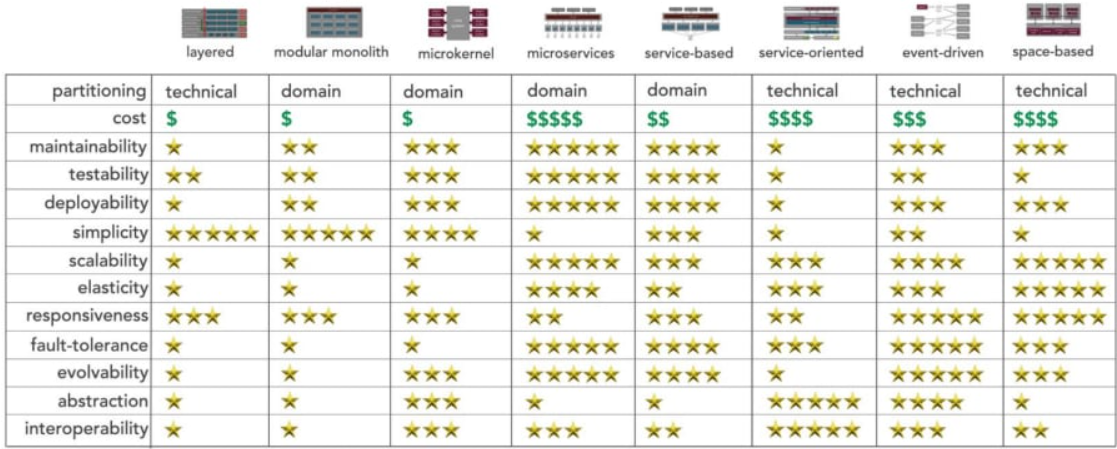
\includegraphics[width=\linewidth]{figures/ch05/architecture/compare-architecture.png}
\caption{So sánh các đặc tính của các kiểu kiến trúc (Nguồn: Mark Richards, Neal Ford, \textit{Fundamentals of Software Architecture}, O'Reilly, 2nd ed., 2020) \cite{Richards2020FSA}.}
\label{fig:compare-architecture}
\end{figure}


\textbf{C. Phân tích loại trừ:}
Từ biểu đồ trên kết hợp với các yêu cầu nghiệp vụ đã xác định, nhóm tiến hành loại trừ các kiến trúc không phù hợp:
\begin{itemize}
    \item \textbf{Loại bỏ Kiến trúc Vi dịch vụ (Microservices):}
    \begin{itemize}
        \item \textit{Ưu điểm từ biểu đồ:} Đạt điểm tuyệt đối về khả năng mở rộng (scalability: 5 sao), triển khai độc lập (deployability: 5 sao), và khả năng chịu lỗi (fault-tolerance: 5 sao).
        \item \textit{Nhược điểm nghiêm trọng:} Chi phí vận hành ở mức cao nhất (\$\$\$\$\$) và độ phức tạp có điểm thấp nhất (simplicity: 1 sao).
        \item \textit{Mâu thuẫn với yêu cầu:} Với nguồn lực hạn chế của đồ án sinh viên, việc vận hành hạ tầng phân tán (service discovery, distributed tracing, container orchestration) là không khả thi. Hơn nữa, các nghiệp vụ mượn/trả sách đòi hỏi cập nhật đồng thời nhiều aggregate (giao dịch, tồn kho, hàng đợi) - nếu tách thành microservices sẽ phải xử lý distributed transactions phức tạp (Saga pattern, 2PC:Two-Phase Commit) với rủi ro eventual consistency.
    \end{itemize}

    \item \textbf{Loại bỏ Kiến trúc Phân lớp (Layered) truyền thống:}
    \begin{itemize}
        \item \textit{Ưu điểm từ biểu đồ:} Đơn giản nhất (simplicity: 5 sao) và chi phí thấp nhất (cost: \$).
        \item \textit{Nhược điểm nghiêm trọng:} Các chỉ số quan trọng cho sự phát triển dài hạn đều ở mức thấp: khả năng bảo trì (maintainability: 1 sao), khả năng kiểm thử (testability: 2 sao), và tính linh hoạt (evolvability: 1 sao).
        \item \textit{Mâu thuẫn với yêu cầu:} Kiến trúc phân lớp theo kỹ thuật (technical layers) dễ dẫn đến tight coupling giữa các logic nghiệp vụ. Đối với hệ thống có yêu cầu tích hợp AI phức tạp (xử lý bất đồng bộ PDF, cập nhật vector embeddings, trigger recommendation engine), kiến trúc này dễ dẫn đến "big ball of mud" với business logic rải rác khắp các layer.
    \end{itemize}

    \item \textbf{Cân nhắc về Kiến trúc Hướng dịch vụ (Service-Based):}
    \begin{itemize}
        \item \textit{Ưu điểm từ biểu đồ:} Sự cân bằng tốt với hầu hết chỉ số đạt 3--4 sao (maintainability: 4 sao, testability: 4 sao, deployability: 4 sao) và chi phí vừa phải (cost: \$\$).
        \item \textit{Hạn chế trong bối cảnh dự án:} Việc tách ngay từ đầu toàn bộ các nghiệp vụ thư viện thành nhiều service riêng biệt (User Service, Catalog Service, Circulation Service, Fine Service) là \textbf{over-engineering} cho giai đoạn MVP. Các service này có phụ thuộc lẫn nhau cao: mượn sách cần kiểm tra tài khoản, tình trạng bản sao, đặt trước và phí phạt. Nếu tách quá sớm, hệ thống sẽ phải đánh đổi bằng nhiều inter-service calls, tăng network latency và độ phức tạp debugging.
        \item \textit{Kết luận:} Service-Based là hướng đi tương lai hợp lý khi hệ thống cần scale, nhưng chưa phù hợp cho giai đoạn đầu.
    \end{itemize}
\end{itemize}

\textbf{D. Quyết định: Kiến trúc Modular Monolith kết hợp Dịch vụ vệ tinh AI}

Dựa trên phân tích trên, nhóm quyết định áp dụng một cách tiếp cận \textbf{thực dụng và có định hướng phát triển}, kết hợp ưu điểm của Modular Monolith với tính linh hoạt của Service-Based Architecture:

\begin{enumerate}
    \item \textbf{Lõi hệ thống: Modular Monolith (Spring Boot)}

    Đây là kiến trúc chủ đạo cho các nghiệp vụ quản lý thư viện (Auth/User, Catalog, Circulation, Fine/Payment, Notification và Engagement).

    \textit{Lý do lựa chọn dựa trên biểu đồ so sánh:}
    \begin{itemize}
        \item \textbf{Cân bằng tối ưu:} Modular Monolith cung cấp maintainability (3 sao) và evolvability (3 sao) tốt hơn hẳn Layered Architecture (1 sao) nhưng vẫn giữ được chi phí thấp (cost: \$) và độ đơn giản cao (simplicity: 5 sao).
        \item \textbf{Testability:} Đạt 3 sao - cao hơn đáng kể so với Layered (2 sao) nhờ tách biệt rõ ràng giữa các domain module.
        \item \textbf{Deployability:} Dù chỉ đạt 3 sao (thấp hơn Microservices), nhưng lại phù hợp với nguồn lực đồ án: chỉ cần deploy một artifact duy nhất, không cần orchestration phức tạp.
    \end{itemize}

    \textit{Lợi ích nghiệp vụ cụ thể:}
    \begin{itemize}
        \item \textbf{Tính nhất quán giao dịch (ACID):} Các use case phức tạp như trả sách (cần atomic update: trạng thái giao dịch + tính phạt + cập nhật tồn kho + trigger hàng đợi) được đảm bảo trong một transaction duy nhất mà không cần distributed transaction protocols.
        \item \textbf{Tính module hóa cao:} Mặc dù là monolith, code được tổ chức theo \textbf{domain boundaries} (không phải technical layers). Mỗi module (Auth/User, Catalog, Circulation, Recommendation...) có domain model, use cases, và repositories riêng, giao tiếp thông qua well-defined interfaces. Điều này tạo "exit strategy" - dễ dàng tách module ra thành service riêng trong tương lai nếu cần.
        \item \textbf{DevOps đơn giản:} Chỉ cần một deployment pipeline, một database connection pool, không cần service mesh hay API gateway phức tạp.
    \end{itemize}

    \item \textbf{Dịch vụ vệ tinh: AI Service (Python/FastAPI)}

    Mô-đun AI/Recommendation System được tách ra thành một dịch vụ độc lập, giao tiếp với Monolith chủ yếu qua REST API. Các tác vụ xử lý PDF được backend kích hoạt bất đồng bộ sau khi lưu URL tài liệu; AI service cũng có khả năng chạy worker nền cho các job xử lý dài nếu cần.

    \textit{Lý do tách riêng:}
    \begin{itemize}
        \item \textbf{Công nghệ khác biệt:} Hệ sinh thái Python (HuggingFace/SentenceTransformer, PyMuPDF, implicit ALS, FastAPI) phù hợp hơn cho ML/NLP so với việc nhúng các thư viện này trực tiếp vào Spring Boot.
        \item \textbf{Scaling requirements khác biệt:} AI workload (PyMuPDF, vector similarity search, model inference) tiêu tốn CPU/GPU nhiều hơn CRUD nghiệp vụ. Tách riêng cho phép scale độc lập (horizontal scaling với GPU instances) mà không tốn tài nguyên cho monolith.
        \item \textbf{Bất đồng bộ tự nhiên:} Xử lý PDF, sinh embedding và gọi Gemini không cần chặn luồng thủ thư upload tài liệu. Backend lưu trạng thái ETL, gọi AI service bằng tác vụ nền và có fallback khi AI lỗi.
        \item \textbf{Tính module hóa:} AI Service dùng schema dữ liệu phục vụ AI như \texttt{ai\_engine.publication\_vectors}, \texttt{publication\_etl\_runs} và bảng \texttt{ai\_recommendations}, nhưng giao tiếp với backend vẫn thông qua API contract rõ ràng. Nhờ đó nhóm có thể thay đổi model embedding hoặc chiến lược recommendation mà không làm xáo trộn nghiệp vụ thư viện.
    \end{itemize}

    \textit{Migration path:} Đây là bước đệm hướng tới Service-Based Architecture. Trong tương lai, nếu cần scale, có thể tách dần các module khác (User Service, Notification Service) ra khỏi monolith theo pattern tương tự.
\end{enumerate}


\textbf{E. Đánh giá kiến trúc lai theo các chỉ số:}
Kiến trúc Modular Monolith + AI Satellite này đạt được sự cân bằng tốt nhất cho bối cảnh dự án:
\begin{table}[H]
\centering
\caption{Đánh giá kiến trúc lai so với các chỉ số}
\begin{tabular}{|l|c|l|}
\hline
\textbf{Tiêu chí} & \textbf{Điểm} & \textbf{Nhận xét} \\ \hline
Cost & \$\$ & Giữa Modular Monolith (\$) và Service-Based (\$\$), phù hợp ngân sách \\ \hline
Simplicity & 3-4 sao & Đơn giản hơn Microservices nhưng cần quản lý 2 components \\ \hline
Maintainability & 3-4 sao & Module hóa domain tốt, dễ sửa lỗi và refactor \\ \hline
Testability & 3 sao & Domain logic tách biệt, dễ unit test \\ \hline
Deployability & 2-3 sao & Deploy 2 artifacts (Monolith + AI), CI/CD đơn giản \\ \hline
Scalability & 3 sao & AI service scale độc lập, monolith scale theo nhu cầu \\ \hline
Evolvability & 4 sao & Có thể tách dần modules ra thành services khi cần \\ \hline
\end{tabular}
\end{table}

\textbf{Kết luận:} Kiến trúc Modular Monolith + AI Satellite Service đạt được ba mục tiêu then chốt: (1) Đảm bảo tính nhất quán giao dịch cho nghiệp vụ core, (2) Tối ưu hóa AI workload với công nghệ và scaling phù hợp, (3) Giữ độ phức tạp và chi phí ở mức chấp nhận được cho đồ án, đồng thời tạo nền tảng để mở rộng thành Service-Based Architecture hoặc Microservice Architecture trong tương lai.


\subsection{Thiết kế cơ sở dữ liệu}
\label{subsec:database-design}

Thiết kế cơ sở dữ liệu là quá trình chuyển đổi từ mô hình phân tích yêu cầu và các thực thể đã được đặc tả ở các phần trước thành một cấu trúc lưu trữ logic và vật lý. Mục tiêu là xây dựng một nền tảng dữ liệu nhất quán, toàn vẹn, hiệu quả và có khả năng mở rộng để hỗ trợ toàn bộ nghiệp vụ của hệ thống, từ các giao dịch mượn trả cơ bản đến các tính năng AI phức tạp.

\subsubsection{Lựa chọn Hệ Quản trị Cơ sở dữ liệu (HQTCSDL)}
Dựa trên bản chất quan hệ chặt chẽ của dữ liệu (người dùng, sách, lượt mượn), hệ thống lựa chọn \textbf{PostgreSQL} làm HQTCSDL chính.
\begin{itemize}
 \item \textbf{Tính tin cậy và toàn vẹn dữ liệu:} PostgreSQL nổi tiếng với sự tuân thủ nghiêm ngặt các tiêu chuẩn ACID (Atomicity, Consistency, Isolation, Durability), đảm bảo các giao dịch nghiệp vụ quan trọng như mượn, trả, và tính phí phạt luôn được thực hiện một cách an toàn.
 \item \textbf{Hỗ trợ các kiểu dữ liệu nâng cao:} PostgreSQL hỗ trợ các kiểu dữ liệu phức tạp như JSONB, rất hữu ích để lưu trữ các metadata linh hoạt. Đặc biệt, thông qua các extension như \texttt{pgvector}, nó có khả năng lưu trữ và truy vấn các vector embedding hiệu quả, phục vụ trực tiếp cho tính năng tìm kiếm ngữ nghĩa.
 \item \textbf{Khả năng mở rộng:} Đây là một hệ quản trị CSDL mã nguồn mở mạnh mẽ, đã được chứng minh về hiệu năng trong các hệ thống quy mô lớn.
\end{itemize}

\subsubsection{Mô hình Quan hệ Thực thể (ERD)}
Bên dưới là sơ đồ ERD tổng quan của toàn bộ hệ thống. Mô hình dữ liệu được
thiết kế xoay quanh thực thể trung tâm là \textbf{Publication} và
\textbf{User}. \textbf{Publication} biểu diễn đầu sách hoặc tài liệu thư viện,
liên kết với tác giả, nhà xuất bản, danh mục, thẻ chủ đề, bản sao vật lý
(\textbf{Item}) và dữ liệu vector phục vụ tìm kiếm ngữ nghĩa. \textbf{User}
liên kết với vai trò, lịch sử tìm kiếm, wishlist, đánh giá, tương tác, thông
báo và các nghiệp vụ mượn/đặt trước.

Các quan hệ nghiệp vụ chính được thể hiện qua \textbf{borrowing\_transactions},
\textbf{reservations} và \textbf{fines}. Một người dùng có thể tạo nhiều phiếu
mượn hoặc đặt trước; mỗi phiếu mượn gắn với một bản sao sách cụ thể và có thể
phát sinh phí phạt nếu quá hạn, mất sách hoặc hư hỏng. Nhóm bảng AI như
\textbf{PublicationVector}, \textbf{Ai\_Recommendation} và
\textbf{user\_interactions} được tách ra nhưng vẫn liên kết với dữ liệu lõi để
hỗ trợ gợi ý cá nhân hóa, tìm kiếm ngữ nghĩa và phân tích hành vi đọc.

\begin{figure}[htbp]
 \centering
\includegraphics[width=1\linewidth]{figures/ch05/database/erd.png}
 \caption{Sơ đồ Quan hệ Thực thể (ERD) tổng thể của hệ thống}
 \label{fig:erd}
\end{figure}
\FloatBarrier

\subsection{Thiết kế chi tiết bên trong}
\subsubsection{Mô hình kiến trúc chi tiết}
Sau khi quyết định sử dụng kiến trúc Modular Monolith kết hợp AI Satellite Service, phần này trình bày chi tiết cấu trúc nội bộ của từng thành phần và các nguyên tắc thiết kế được áp dụng.

\textbf{A. Tổng quan kiến trúc hệ thống:}
\begin{figure}[htbp]
 \centering
 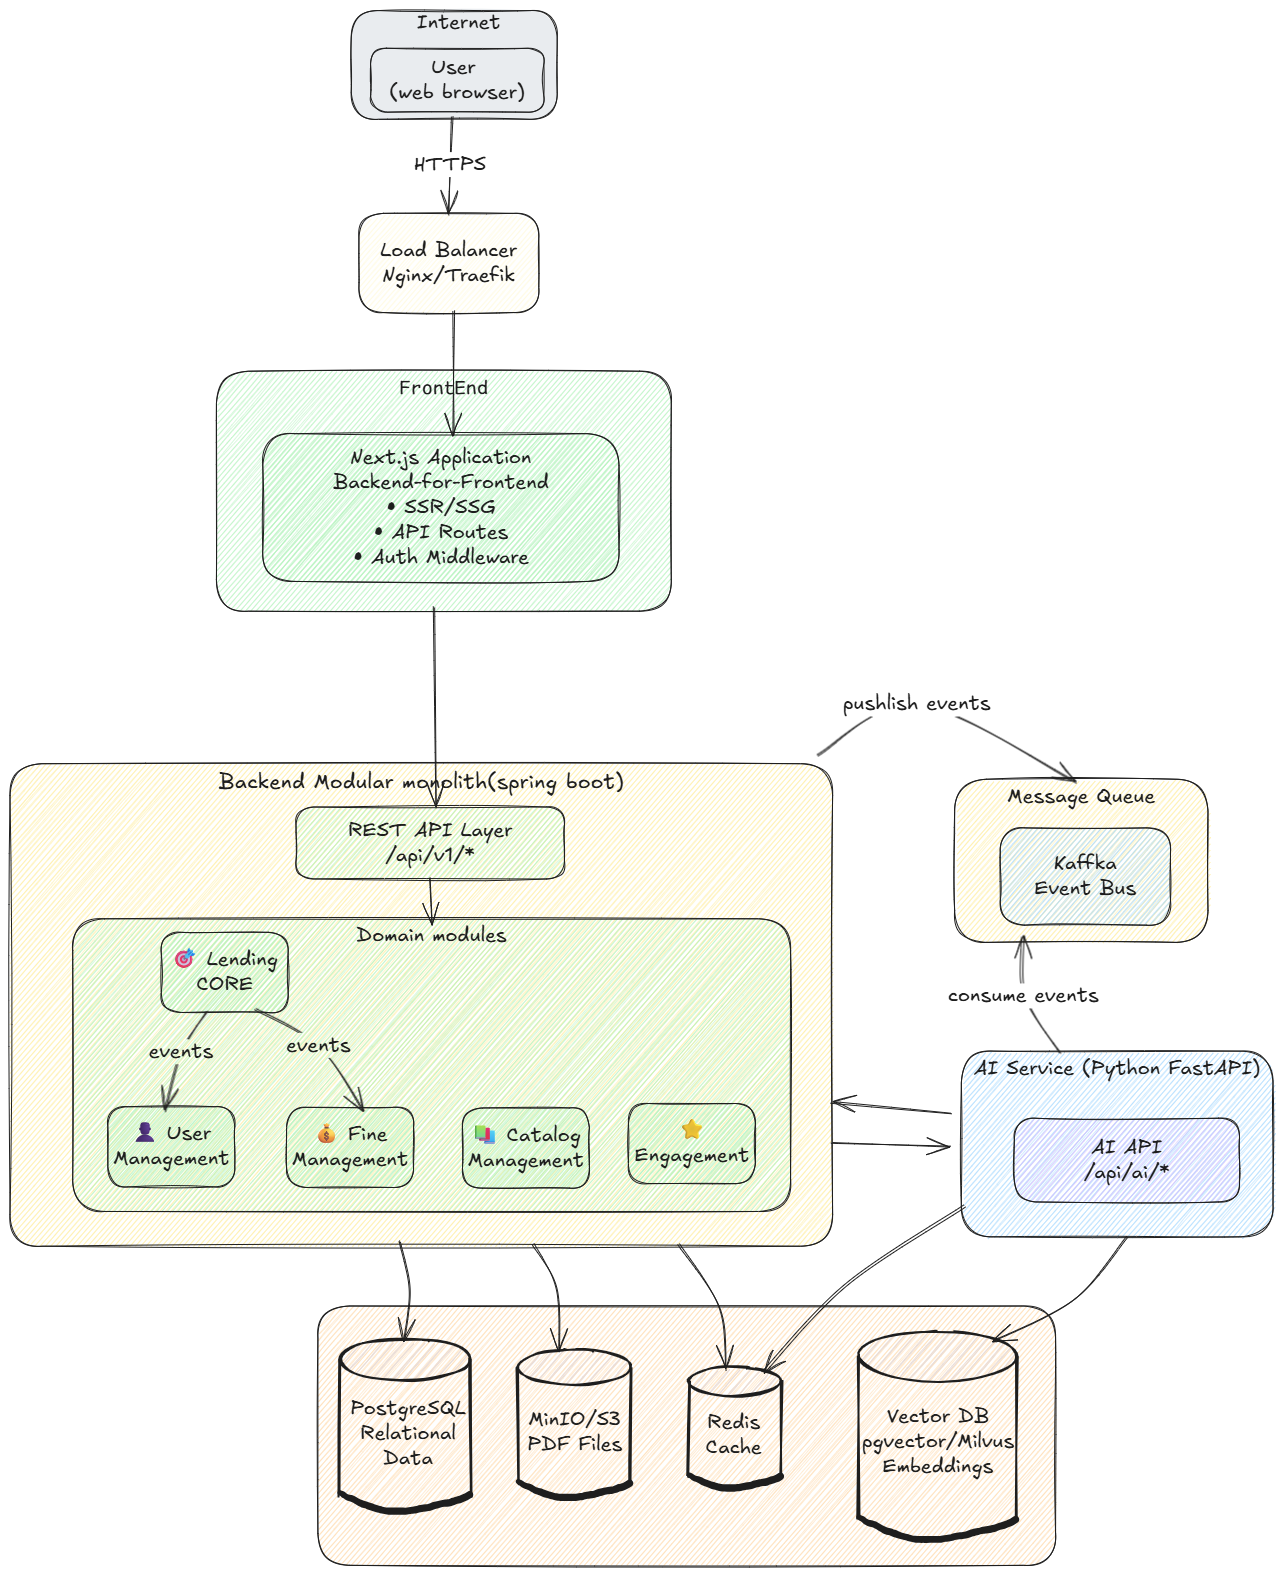
\includegraphics[width=1\linewidth]{figures/ch05/architecture/system_architecture_overview.png}
 \caption{Sơ đồ kiến trúc tổng thể hệ thống}
 \label{fig:system_architecture_overview}
\end{figure}
Hệ thống bao gồm ba thành phần chính:
\begin{enumerate}
    \item \textbf{Frontend (React/Vite SPA):} Giao diện người dùng chạy phía trình duyệt, tổ chức route cho public, reader, librarian và admin, gọi REST API trực tiếp đến backend.
    \item \textbf{Backend Monolith (Spring Boot):} Lõi nghiệp vụ áp dụng Domain-Driven Design và Clean Architecture.
    \item \textbf{AI Service (Python FastAPI):} Dịch vụ độc lập xử lý các tác vụ Machine Learning và Vector Search.
\end{enumerate}


\textbf{B. Kiến trúc Backend Monolith (Spring Boot)}
\textbf{Tổ chức theo Bounded Contexts (DDD):}

Thay vì tổ chức code theo các lớp kỹ thuật ngang (technical layers), hệ thống được chia thành các module theo ranh giới nghiệp vụ (domain boundaries), mỗi module tương ứng với một Bounded Context trong Domain-Driven Design:

\begin{figure}[htbp]
 \centering
 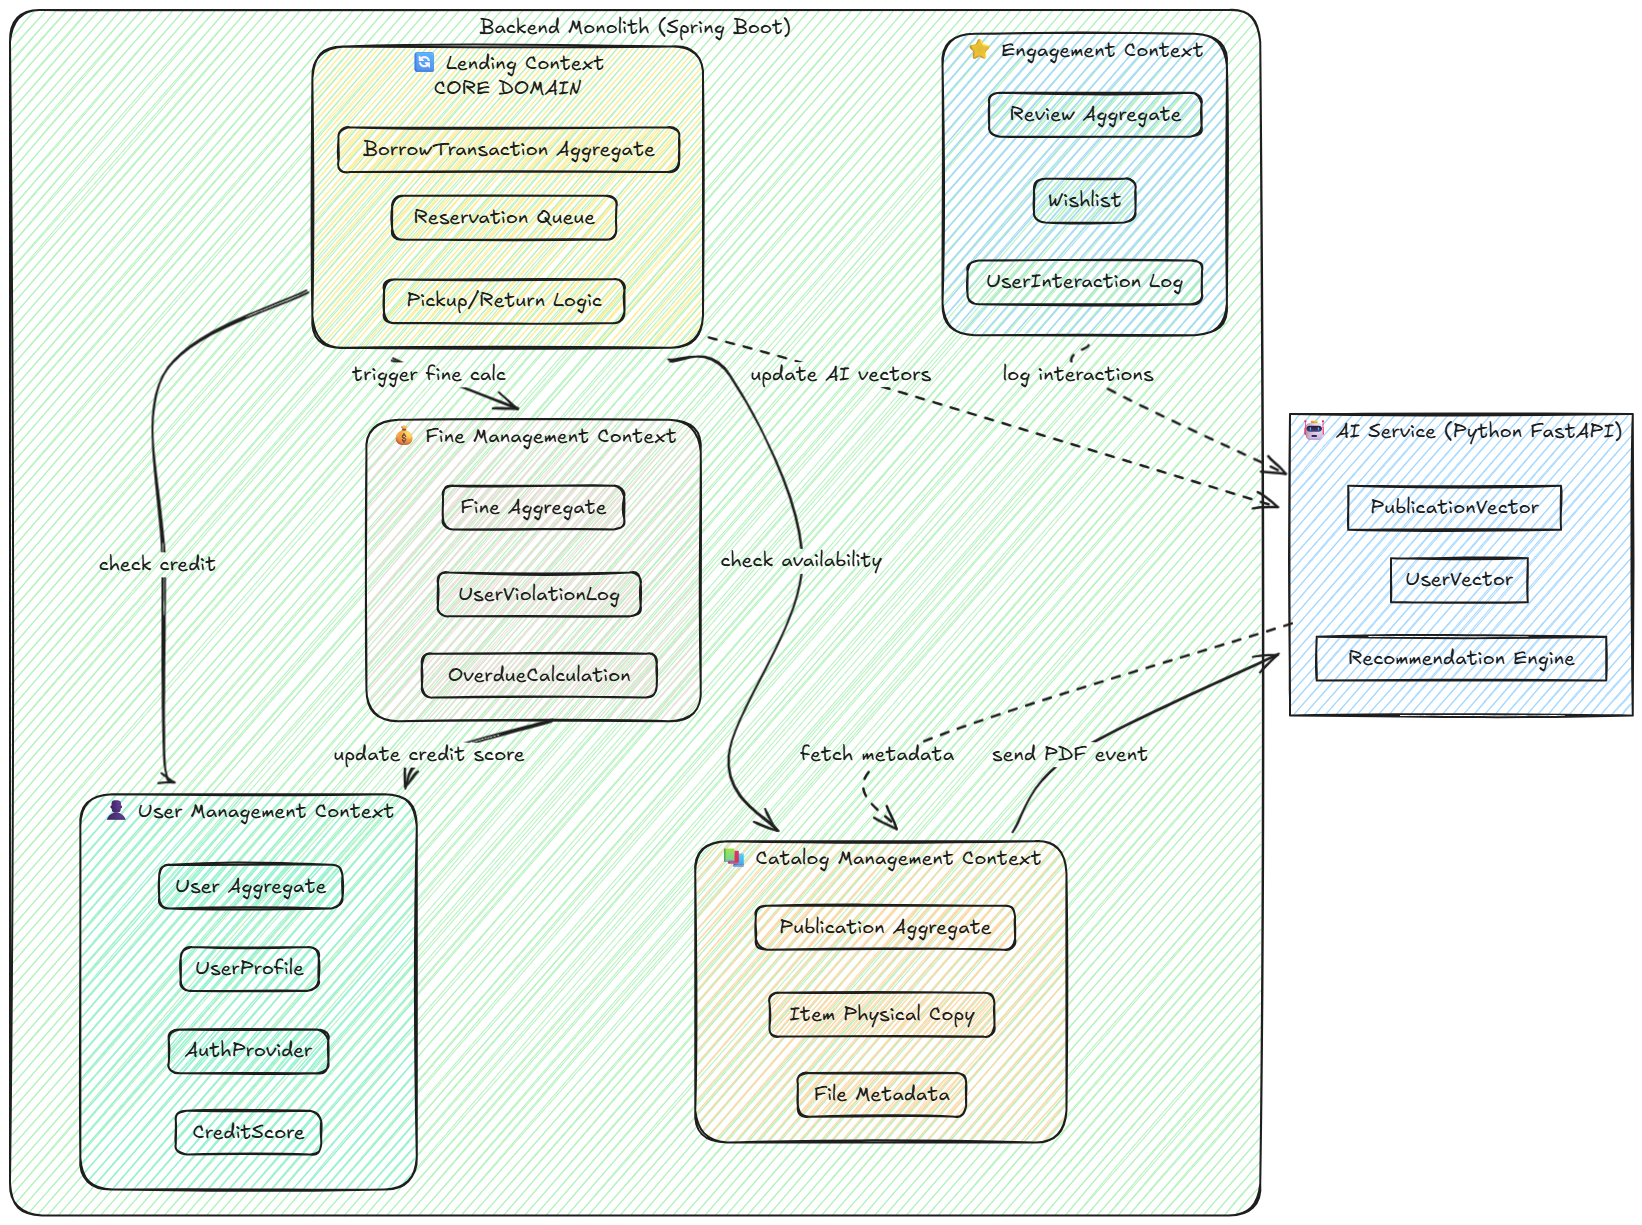
\includegraphics[width=1\linewidth]{figures/ch05/architecture/bounded_contexts.png}
 \caption{Các Bounded Contexts trong hệ thống}
 \label{fig:bounded_contexts}
\end{figure}

\begin{itemize}
    \item \textbf{Auth/User Management Context:} Quản lý đăng ký, đăng nhập, xác thực email, Google OAuth, hồ sơ người dùng, vai trò và phân quyền.
    \item \textbf{Catalog Management Context:} Quản lý thông tin xuất bản phẩm (Publication), các bản sao vật lý (Item), metadata sách, và file storage.
    \item \textbf{Circulation Context:} \textit{(Core Domain)} - Quản lý vòng đời mượn/trả sách (BorrowingTransaction), yêu cầu mượn, xác nhận nhận sách, hàng đợi đặt trước (Reservation), trả sách và báo cáo sách hư/mất.
    \item \textbf{Fine/Payment Context:} Quản lý phí quá hạn, phí sự cố, thanh toán tiền mặt, thanh toán PayOS và đồng bộ trạng thái webhook.
    \item \textbf{Engagement/Recommendation Context:} Quản lý đánh giá sách, phản hồi review, danh sách yêu thích, lịch sử tìm kiếm, log tương tác người dùng, semantic search và recommendation.
    \item \textbf{Notification Context:} Lưu thông báo, đếm thông báo chưa đọc và đẩy realtime qua WebSocket/STOMP.
\end{itemize}

Mỗi Bounded Context được thiết kế như một "mini-service" bên trong monolith, có thể tách ra thành service độc lập trong tương lai mà không cần refactor lớn.

\textbf{Clean Architecture bên trong mỗi Module:}

Bên trong mỗi Bounded Context, code được tổ chức theo 4 layers của Clean Architecture để đảm bảo tách biệt trách nhiệm và independence từ framework/database:
\begin{figure}[htbp]
 \centering
 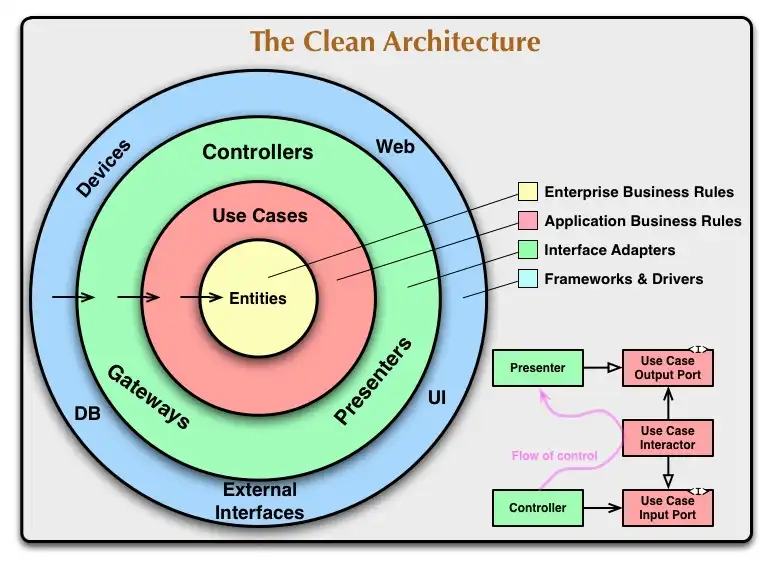
\includegraphics[width=1\linewidth]{figures/ch05/architecture/clean-architecture.png}
 \caption{Clean architecture (R. C. Martin, \textit{Clean Architecture: A Craftsman’s Guide to Software Structure and Design},  Pearson Education, 2018 \cite{martin2018clean})}
 \label{fig:clean_architecture_layers}
\end{figure}
\begin{figure}[htbp]
 \centering
 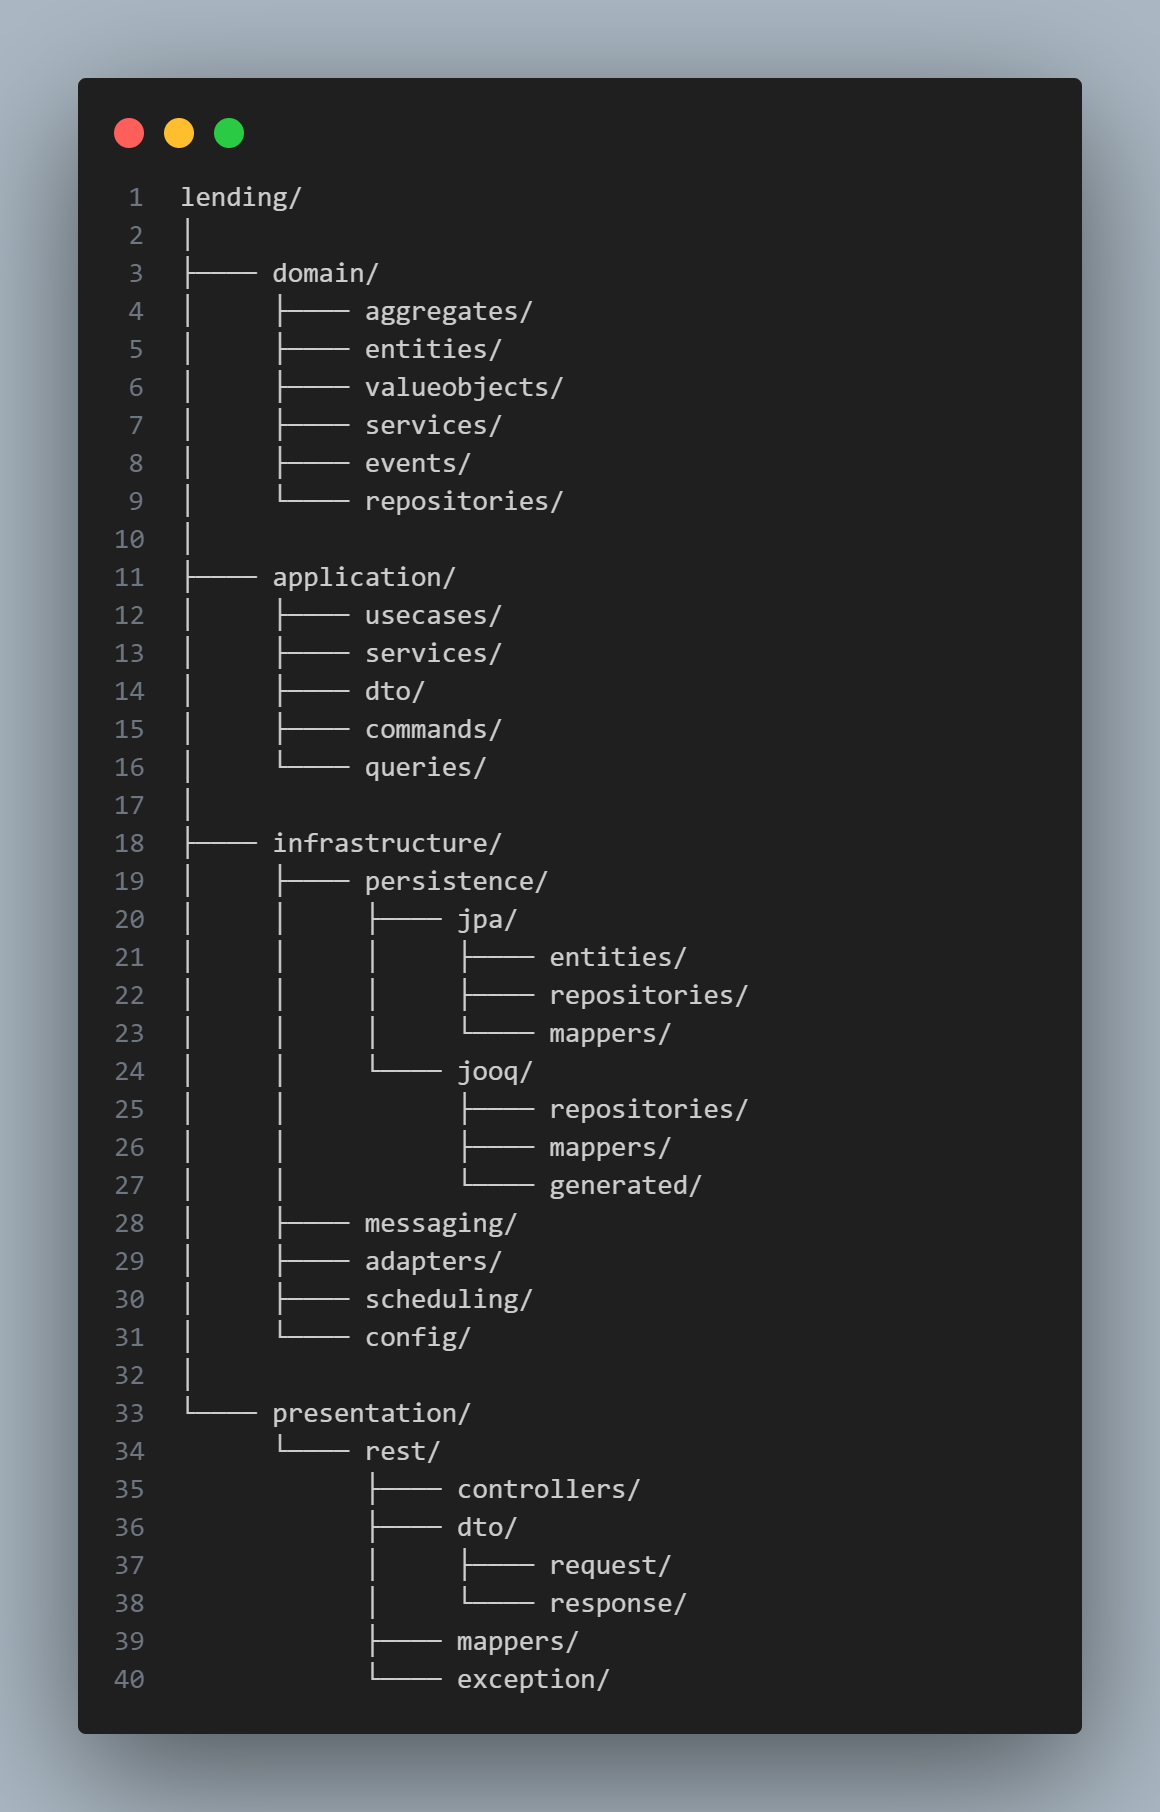
\includegraphics[width=0.8\linewidth]{figures/ch05/architecture/folder_structure_backend.png}
 \caption{Cấu trúc Clean Architecture kết hợp Domain-Driven Design trong một Module}
 \label{fig:clean_architecture_in_module}
\end{figure}

\textbf{1. Domain Layer (Lõi nghiệp vụ - Innermost):}
\begin{itemize}
    \item \textbf{Entities và Aggregates:} Chứa các đối tượng nghiệp vụ cốt lõi với business invariants. Ví dụ:
    \begin{itemize}
        \item \texttt{BorrowingTransaction} Aggregate: Đảm bảo vòng đời giao dịch từ yêu cầu mượn, xác nhận nhận sách, đang mượn, trả sách đến báo cáo sự cố.
        \item \texttt{Publication} Aggregate: Đảm bảo metadata ấn phẩm nhất quán, liên kết đúng tác giả, nhà xuất bản, danh mục, tag, ảnh bìa và tài liệu PDF.
        \item \texttt{Item} Aggregate: Đảm bảo mỗi bản sao có barcode riêng, trạng thái riêng và chỉ được mượn khi đang khả dụng.
    \end{itemize}

    \item \textbf{Value Objects:} Các đối tượng bất biến đại diện cho khái niệm nghiệp vụ không có identity riêng, ví dụ \texttt{Barcode}, \texttt{PublicationId}, \texttt{ItemId} hoặc trạng thái bản sao.

    \item \textbf{Domain Services:} Logic nghiệp vụ thuần không thuộc về một Entity/Aggregate cụ thể. Ở mức thiết kế, nhóm dự kiến đặt tại đây các quy tắc có thể dùng lại như:
    \begin{itemize}
        \item Tính số ngày quá hạn và xác định loại phí phát sinh theo chính sách lưu thông.
        \item Chọn bản sao phù hợp cho yêu cầu đặt trước dựa trên trạng thái bản sao, chi nhánh và thứ tự hàng đợi.
    \end{itemize}

    \item \textbf{Domain Events:} Biểu diễn các sự kiện nghiệp vụ quan trọng để application/infrastructure có thể phản ứng mà không làm domain phụ thuộc vào công nghệ cụ thể:
    \begin{itemize}
        \item Sự kiện mượn/trả, phát sinh phí phạt, thay đổi trạng thái đặt trước.
        \item Sự kiện yêu cầu gửi thông báo/email sau khi transaction nghiệp vụ hoàn tất.
        \item Sự kiện thay đổi trạng thái xử lý tài liệu sau khi pipeline AI hoàn tất hoặc thất bại.
    \end{itemize}

    \item \textbf{Repository Interfaces:} Domain định nghĩa các interface (contract) mà Infrastructure sẽ implement. Domain không quan tâm dùng JPA, JDBC hay MongoDB.

    \item \textbf{Ràng buộc nghiêm ngặt:} Domain Layer KHÔNG ĐƯỢC phụ thuộc vào bất kỳ layer nào khác, không import Spring annotations, không biết HTTP hay Database. Đây là "business logic in pure Java".
\end{itemize}

\textbf{2. Application Layer (Use Cases - Orchestrator):}
\begin{itemize}
    \item \textbf{Use Case Services:} Mỗi use case là một entry point cho một chức năng nghiệp vụ hoàn chỉnh. Ví dụ:
    \begin{itemize}
        \item \texttt{BorrowRequestUseCase}: Điều phối luồng gửi yêu cầu mượn từ bạn đọc.
        \item \texttt{BorrowDirectUseCase}: Điều phối luồng thủ thư cho mượn trực tiếp tại quầy.
        \item \texttt{ConfirmPickupUseCase}: Xác nhận bạn đọc đã nhận sách sau khi có yêu cầu mượn hoặc đặt trước.
        \item \texttt{ReturnBookUseCase}: Điều phối luồng trả sách, cập nhật bản sao và tính phí quá hạn nếu có.
        \item \texttt{ReportIssueUseCase}: Ghi nhận sách hư/mất và tạo phí sự cố.
    \end{itemize}

    \item \textbf{Trách nhiệm chính:}
    \begin{itemize}
        \item Orchestrate workflow: Gọi repositories để load aggregates, gọi domain services, và save kết quả.
        \item Quản lý transaction boundaries (sử dụng \texttt{@Transactional} annotation của Spring).
        \item Kích hoạt các side effect cần thiết như notification, email hoặc cập nhật trạng thái AI thông qua adapter tương ứng.
        \item Transform exceptions: Chuyển domain exceptions thành application-level error codes.
    \end{itemize}

    \item \textbf{Application Services:} Các facade cho phép module khác gọi vào (public API giữa các modules).

    \item \textbf{DTOs (Data Transfer Objects):} Chuyển đổi giữa domain objects và external representations (JSON, DTO cho API).

    \item \textbf{Lưu ý:} Application Layer được phép phụ thuộc vào Domain Layer và định nghĩa interfaces cho Infrastructure (Dependency Inversion Principle).
\end{itemize}


\textbf{3. Infrastructure Layer (Technical Implementation - Outermost):}
\begin{itemize}
    \item \textbf{Repository Implementations:} Hiện thực các repository interfaces từ Domain bằng JPA/Hibernate, JDBC, hoặc bất kỳ persistence technology nào. Ví dụ:
    \begin{itemize}
        \item \texttt{BorrowingTransactionJpaRepository}: Truy vấn và cập nhật giao dịch mượn--trả.
        \item Mapping giữa domain/use case và JPA Entity như \texttt{BorrowingTransactionEntity}, \texttt{FineEntity}, \texttt{PublicationEntity}.
    \end{itemize}

    \item \textbf{External Service Adapters:} Tích hợp với các dịch vụ bên ngoài:
    \begin{itemize}
        \item Email/SMS Service (gửi notification)
        \item File Storage (S3-compatible storage để lưu ảnh bìa và PDF)
        \item Payment Gateway (PayOS cho thanh toán phạt trực tuyến)
        \item OAuth Provider (Google Authentication)
    \end{itemize}

    \item \textbf{Event Infrastructure:} Hiện thực event publishing/subscribing:
    \begin{itemize}
        \item Kafka producer/consumer cho notification, email và các tác vụ cần tách khỏi request chính.
        \item REST client đến AI Service cho semantic search, recommendation và xử lý PDF.
    \end{itemize}

    \item \textbf{Technical Services:}
    \begin{itemize}
        \item Scheduler (Spring \texttt{@Scheduled}) cho background jobs (check overdue daily).
        \item WebSocket/STOMP cho thông báo realtime.
        \item Security (JWT token generation/validation, password hashing).
    \end{itemize}

    \item \textbf{Configuration:} Database connection pools, Kafka/WebSocket configuration, S3, PayOS, AI gateway, security settings.
\end{itemize}


\textbf{4. Presentation Layer (Interface Adapters):}
\begin{itemize}
    \item \textbf{REST Controllers:} Expose các use cases qua HTTP/REST API. Mỗi Bounded Context có controller riêng:
    \begin{itemize}
        \item \texttt{UserController} (\texttt{/api/v1/users/*})
        \item \texttt{PublicationController} (\texttt{/api/v1/publications/*})
        \item \texttt{BorrowingTransactionController} (\texttt{/api/v1/transactions/*})
        \item \texttt{ReservationController} (\texttt{/api/v1/reservations/*})
        \item \texttt{FineController} (\texttt{/api/v1/fines/*})
        \item \texttt{RecommendationController} (\texttt{/api/v1/recommendations/*})
        \item \texttt{AiSearchController} (\texttt{/api/v1/ai/semantic-search})
    \end{itemize}

    \item \textbf{Trách nhiệm:}
    \begin{itemize}
        \item Nhận HTTP requests, validate syntax (JSON format, required fields, regex).
        \item Chuyển đổi Request DTOs → Commands/Queries cho Application Layer.
        \item Authentication \& Authorization: Extract user info từ JWT, check permissions.
        \item Chuyển đổi kết quả từ Application Layer → HTTP Response (JSON).
        \item Error handling: Chuyển exceptions thành HTTP status codes (400, 401, 403, 404, 500).
    \end{itemize}

    \item \textbf{Nguyên tắc:} Controllers phải "thin" - chỉ làm việc chuyển đổi và delegation, KHÔNG chứa business logic.
\end{itemize}

\textbf{Dependency Rule (Nguyên tắc phụ thuộc):}
Clean Architecture tuân thủ nguyên tắc: \textbf{Dependencies chỉ được point inward} (từ ngoài vào trong):

\begin{center}
\texttt{Presentation → Application → Domain ← Infrastructure}
\end{center}

\begin{itemize}
    \item Domain Layer: Không phụ thuộc vào ai (pure business logic).
    \item Application Layer: Chỉ phụ thuộc Domain, định nghĩa interfaces cho Infrastructure.
    \item Infrastructure \& Presentation: Phụ thuộc cả Domain và Application, implement interfaces.
\end{itemize}

Điều này đảm bảo business logic (Domain) không bị "ô nhiễm" bởi framework, database hay HTTP concerns.


%-----------------------------AI-----------------------------------


\textbf{C. Kiến trúc AI Service (Python FastAPI)}
Hệ thống AI Service được thiết kế như một \textit{Dịch vụ Vệ tinh Độc lập} (AI Satellite Service), tách biệt khỏi khối Monolith (Spring Boot). Quyết định này nhằm tận dụng sức mạnh của hệ sinh thái Python trong các tác vụ Học máy (Machine Learning) và Xử lý ngôn ngữ tự nhiên (NLP), đồng thời đảm bảo khả năng mở rộng độc lập cho các tác vụ tính toán nặng.
\textbf{C.1. Chiến lược thiết kế và Lựa chọn công nghệ}
Khác với Backend chính tập trung vào tính toàn vẹn dữ liệu giao dịch, AI Service tập trung vào hiệu năng tính toán ma trận và xử lý bất đồng bộ.
\begin{itemize}
\item \textbf{Web Framework - FastAPI:} Được lựa chọn thay vì Flask/Django vì nhẹ, dễ định nghĩa API contract, hỗ trợ Pydantic để kiểm soát dữ liệu đầu vào và phù hợp với các endpoint inference như semantic search, recommendation và publication processing.
\item \textbf{Kiến trúc Phi trạng thái (Stateless):} AI Service không lưu trữ session người dùng. Mọi trạng thái cần thiết được truyền qua payload của request hoặc truy xuất từ PostgreSQL/model artifact, giúp dễ dàng mở rộng theo chiều ngang (Horizontal Scaling) bằng cách tăng số lượng container.
\end{itemize}
\textbf{C.2. Cấu trúc Phân tầng (Layered Architecture)} \\
Kiến trúc nội bộ của AI Service được tinh gọn thành 3 tầng chính để tối ưu hóa đường đi của dữ liệu: \\
\textbf{a. API Layer (Giao tiếp \& Định tuyến):}
\begin{itemize}
\item \textit{Semantic Search Router:} \texttt{POST /api/v1/semantic-search}
\begin{itemize}
\item Xử lý truy vấn tìm kiếm bằng ngôn ngữ tự nhiên.
\item Pipeline: Tiền xử lý text $\rightarrow$ Encoding $\rightarrow$ Vector Search.
\end{itemize}
\item \textit{Recommendation Router:} \texttt{POST /api/v1/recommendations}
\begin{itemize}
\item Trả về danh sách gợi ý cá nhân hóa dựa trên ngữ cảnh (Trang chủ, Chi tiết sách).
\item Có thể mở rộng thêm endpoint làm mới gợi ý theo người dùng khi cần cập nhật mô hình hoặc dữ liệu tương tác.
\end{itemize}
\item \textit{Similar Publications Router:} \texttt{GET /api/v1/publications/\{publicationId\}/similar}
\begin{itemize}
\item Trả về các ấn phẩm tương tự với một sách cụ thể, phục vụ khối gợi ý ở trang chi tiết sách.
\end{itemize}
\item \textit{Data Ingestion Router:} \texttt{POST /api/v1/publications/process}
\begin{itemize}
\item Endpoint nhận yêu cầu xử lý tài liệu mới, trích xuất text PDF, sinh metadata AI và lưu embedding.
\end{itemize}
\end{itemize}
\textbf{b. Service Layer (Logic nghiệp vụ ML):}
Đây là trái tim của hệ thống, chứa các pipeline xử lý dữ liệu phức tạp:
\begin{itemize}
\item \textbf{Embedding Service:} Sử dụng mô hình \texttt{bkai-foundation-models/vietnamese-bi-encoder} hoặc mô hình tương đương để chuyển đổi văn bản tiếng Việt thành vector 768 chiều. Mô hình được load một lần khi service/worker khởi động để giảm độ trễ suy luận.
\item \textbf{PDF Processing Pipeline:}
\begin{itemize}
\item \textit{Extraction:} Sử dụng \textbf{PyMuPDF} để trích xuất văn bản tốc độ cao (nhanh hơn 10x so với pypdf).
\item \textit{Chunking:} Áp dụng chiến lược Cửa sổ trượt theo ký tự với kích thước chunk 1500 và overlap 150 để bảo toàn ngữ cảnh giữa các đoạn cắt.
\item \textit{Metadata Reduce:} Chọn các chunk đại diện, gửi một prompt chính đến Gemini để tạo summary, audience và tag; nếu Gemini lỗi, hệ thống dùng fallback deterministic.
\end{itemize}
\item \textbf{Recommendation Engine:} Sử dụng thư viện \textbf{implicit} để huấn luyện mô hình ALS cho dữ liệu phản hồi ẩn, kết hợp thêm content-based recommendation và trending fallback cho người dùng mới hoặc dữ liệu ít.
\end{itemize}
\textbf{c. Data \& Storage Layer:}
\begin{itemize}
\item \textbf{Vector Database (PostgreSQL + pgvector):} Lưu trữ embeddings của các chunk nội dung PDF. Sử dụng chỉ mục \textbf{HNSW} (Hierarchical Navigable Small World) để tối ưu hóa tốc độ tìm kiếm láng giềng gần nhất (ANN) thay vì quét toàn bộ bảng.
\item \textbf{Model Store:} Các mô hình nặng (SBERT) được tải sẵn vào RAM khi khởi động (Pre-loaded) để giảm độ trễ (Latency).
\item \textbf{Recommendation Store:} Mô hình ALS sau khi huấn luyện được lưu dưới dạng artifact \texttt{.pkl}; kết quả gợi ý gần nhất có thể được lưu lại trong PostgreSQL để backend có dữ liệu fallback khi AI service tạm thời không phản hồi.
\end{itemize}


\begin{figure}[htbp]
\centering
\resizebox{\textwidth}{!}{%
    \begin{tikzpicture}[
      node distance=2.5cm and 2cm,
      auto,
      % Styles
      user/.style={
        rectangle, draw, rounded corners,
        minimum width=2.5cm, minimum height=1.2cm,
        fill=blue!5, align=center, font=\normalsize
      },
      service/.style={
        rectangle, draw, rounded corners,
        minimum width=3.5cm, minimum height=1.5cm,
        fill=gray!10, align=center, font=\normalsize
      },
      db/.style={
        cylinder, shape border rotate=90,
        draw, minimum height=1.5cm,
        minimum width=2cm, align=center,
        fill=orange!10, font=\small, aspect=0.25
      },
      queue/.style={
        rectangle, draw, dashed,
        minimum width=3cm, minimum height=1.2cm,
        fill=red!5, align=center, font=\normalsize
      },
      sync_arrow/.style={
        ->, thick, draw=blue!70, >=stealth
      },
      async_arrow/.style={
        ->, thick, dashed, draw=red!70, >=stealth
      },
      label_text/.style={
        font=\small, align=center, auto=false, fill=white, inner sep=1pt
      }
    ]

    % --- 1. NODES (KHỐI) ---

    % Main flow
    \node[user] (user) {User\\(Browser)};
    \node[service, right=of user] (frontend) {Frontend\\(React/Vite)};
    \node[service, right=of frontend] (backend) {Core Backend\\(Spring Boot)};

    % AI service
    \node[service, below=5cm of backend, fill=green!5, draw=green!60!black] (ai_api) {AI Service API\\(FastAPI)};
    \node[service, below=0.8cm of ai_api, fill=green!5, draw=green!60!black] (ai_worker) {AI Pipeline\\(PDF/Embed)};

    % Group AI
    \node[fit=(ai_api)(ai_worker), draw=green!60!black, dashed, inner sep=0.5cm, label={[green!60!black]above left:\textbf{AI Service}}] (ai_group) {};

    % Async trigger: backend gọi AI sau khi lưu document URL
    \node[queue, right=of backend, xshift=0.5cm, yshift=-2.5cm] (rabbitmq) {Queue/Callback\\(RabbitMQ/Celery)};

    % Storage layer
    \node[db, right=of ai_api, xshift=4.5cm] (pgvector) {Vector DB\\(pgvector)};

    % Metadata and file storage
    \node[db, above=2.5cm of pgvector] (redis) {PostgreSQL\\Metadata};
    \node[db, below=2.5cm of pgvector] (minio) {File Storage\\(S3-compatible)};

    % --- 2. EDGES (KẾT NỐI) ---

    % Synchronous flow
    \draw[sync_arrow] (user) -- node[below] {HTTP} (frontend);
    \draw[sync_arrow] (frontend) -- (backend);

    % Backend -> AI API
    \draw[sync_arrow] (backend) to[bend right=40] node[left, label_text, pos=0.5, xshift=-0.3cm] {1. Search/Rec Req} (ai_api);

    % AI API -> VectorDB
    \draw[sync_arrow] (ai_api) -- node[above, label_text] {2. Query} (pgvector);

    % AI API -> Metadata
    \draw[sync_arrow] (ai_api) |- node[near end, left, label_text, yshift=-0.5cm] {Metadata} (redis);

    % Asynchronous flow

    % A. Backend -> Async trigger
    \draw[async_arrow] (backend) to[bend left=20] node[right, label_text, pos=0.6, xshift=0.2cm] {A. Process PDF} (rabbitmq);

    % B. Trigger -> Worker
    % Đi vòng cung lớn để tránh đè lên chữ khác
    \draw[async_arrow] (rabbitmq.east) to[bend left=50] node[right, label_text, pos=0.5] {B. Execute} (ai_worker.east);

    % C. Pipeline -> File Storage
    \draw[async_arrow] (ai_worker) to[bend right=20] node[below, label_text] {C. Fetch PDF} (minio);

    % D. Worker -> VectorDB
    \draw[async_arrow] (ai_worker) to[bend right=25] node[right, label_text, pos=0.4] {D. Save Vectors} (pgvector);

    % Legend
    \node[draw, fill=white, font=\small, inner sep=6pt,
          below=1cm of minio, xshift=-2cm, anchor=north] {
        \begin{tabular}{@{}l@{\hspace{6pt}}l@{}}
        \tikz[baseline=-0.5ex]{\draw[sync_arrow] (0,0) -- (0.8,0);} & Sync (REST) \\[4pt]
        \tikz[baseline=-0.5ex]{\draw[async_arrow] (0,0) -- (0.8,0);} & Async (Background)
        \end{tabular}
    };

    \end{tikzpicture}
}
\caption{Sơ đồ luồng dữ liệu và Kiến trúc chi tiết AI Service}
\label{fig:ai_service_architecture_diagram}
\end{figure}



\textbf{Sơ đồ chi tiết AI Service} \\
\begin{figure}[htbp]
\centering
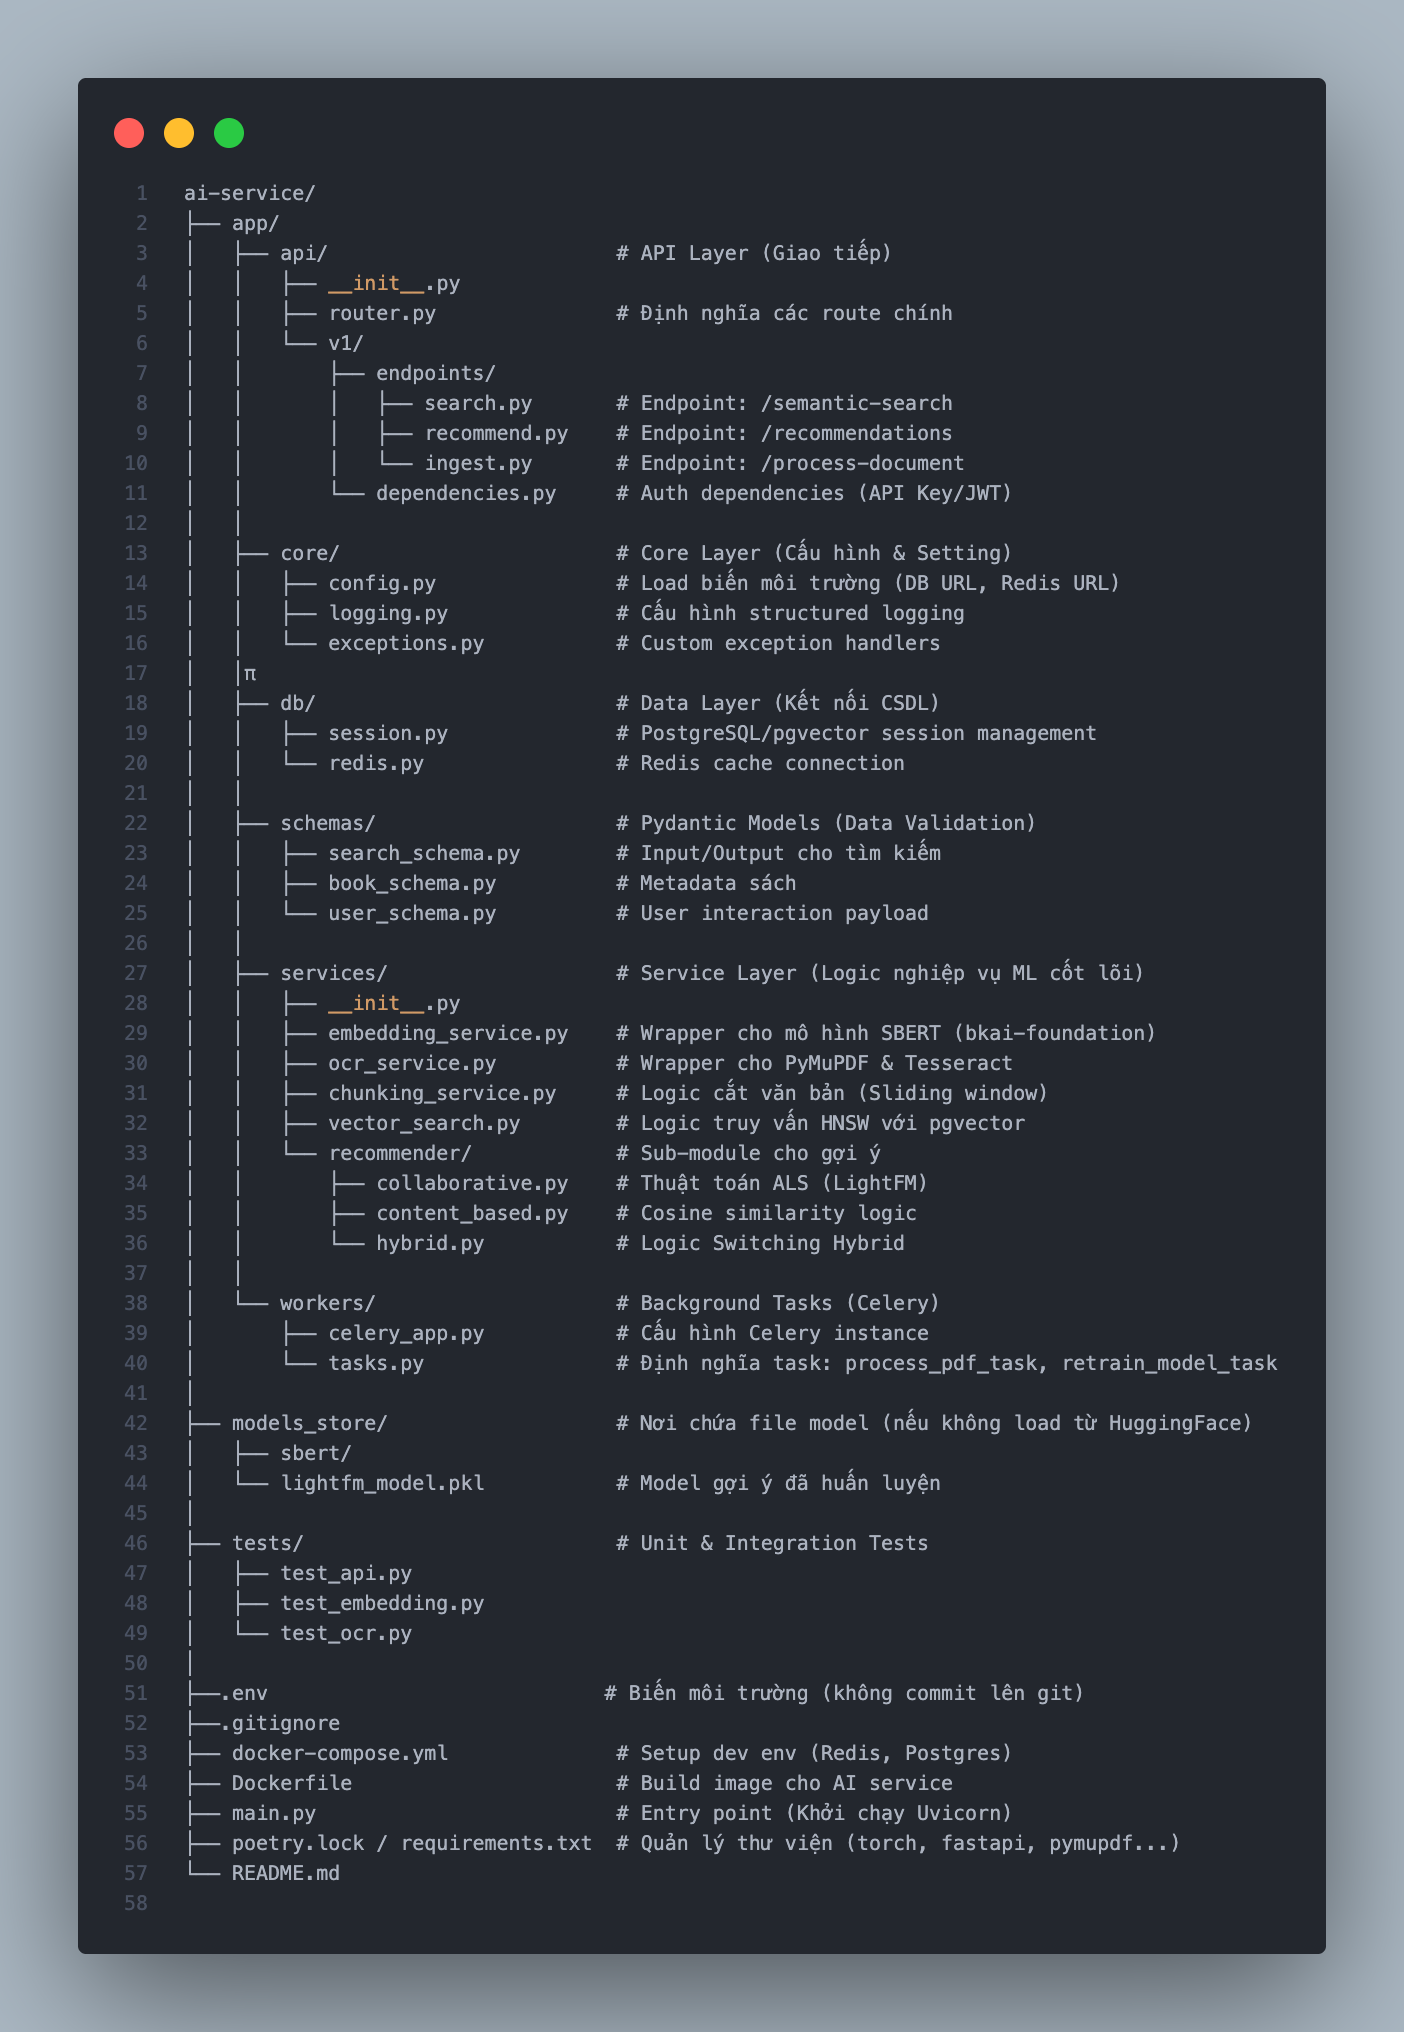
\includegraphics[width=0.95\linewidth]{figures/ch05/architecture/ai_service_architecture.png}
\caption{Kiến trúc chi tiết AI Service và Luồng dữ liệu}
\label{fig:ai_service_architecture_detail}
\end{figure}


%-----------------------------AI-----------------------------------


\subsubsection{Luồng giao tiếp (Communication Flows) nâng cao}

Hệ thống sử dụng hai pattern giao tiếp chính: \textbf{Synchronous Communication} (REST API) cho các tương tác cần phản hồi ngay, và \textbf{Asynchronous Communication} cho các tác vụ không nên chặn luồng nghiệp vụ chính. Ở mức thiết kế, giao tiếp bất đồng bộ được tách thành ba nhóm: Kafka/WebSocket cho notification nội bộ, scheduler/executor cho tác vụ định kỳ hoặc nền trong backend, và queue/callback cho pipeline AI xử lý tài liệu.

\textbf{1. Giao tiếp đồng bộ (Synchronous Communication - REST API):}

Được sử dụng khi:
\begin{itemize}
    \item Frontend cần phản hồi ngay lập tức để hiển thị cho người dùng.
    \item Thao tác đọc dữ liệu (queries) không có side effects.
    \item Validation errors cần trả về trực tiếp cho người dùng.
    \item Cần đảm bảo transaction hoàn thành trước khi tiếp tục workflow.
\end{itemize}

\textbf{Ví dụ 1: Semantic Search Flow}
Luồng tìm kiếm ngữ nghĩa yêu cầu phản hồi nhanh để UX tốt:

\begin{enumerate}
    \item User nhập query "sách về machine learning" trên giao diện tìm kiếm.

    \item \texttt{React/Vite Frontend} gửi \texttt{POST /api/v1/ai/semantic-search} đến Backend Monolith với payload JSON chứa query string và limit.

   \item \texttt{Backend} (\texttt{AiSearchController}/\texttt{AiGatewayService}) xử lý:
    \begin{itemize}
        \item Validate JWT token và extract user info.
        \item Validate query và giới hạn số lượng kết quả.
        \item Chuyển tiếp query sang AI Service qua \texttt{AiGatewayService}; lịch sử tìm kiếm được ghi nhận ở luồng frontend/backend riêng khi người dùng thực hiện tìm kiếm.
        \item Forward request đến AI Service qua internal network.
    \end{itemize}

    \item \texttt{Backend} gọi \texttt{POST http://ai-service:8000/api/v1/semantic-search}
    (internal URL, không expose ra internet).

    \item \texttt{AI Service} xử lý:
    \begin{itemize}
        \item Embedding Service chuyển query thành vector 768 chiều.
        \item Vector Search Service thực hiện ANN search trên bảng vector chunk bằng pgvector.
        \item Gom các chunk gần nhất về danh sách publication IDs với similarity scores.
    \end{itemize}

    \item \texttt{Backend} nhận response từ AI Service:
    \begin{itemize}
        \item Kiểm tra lỗi/timeout từ AI service và fallback sang tìm kiếm catalog nếu cần.
        \item Log request (userId, query, resultCount, responseTime) để phân tích.
    \end{itemize}

    \item \texttt{Backend} query PostgreSQL để lấy metadata chi tiết
    (title, author, cover, availability) của các publication IDs.

    \item \texttt{Backend} merge AI results + metadata, trả về Frontend.

    \item Frontend render kết quả tìm kiếm.
\end{enumerate}

\textbf{Đặc điểm kỹ thuật:}
\begin{itemize}
    \item \textbf{Request-Response pattern:} Client chờ response trước khi tiếp tục (blocking call).
    \item \textbf{Timeout handling:} Backend cấu hình timeout khi gọi AI service để tránh làm treo request người dùng.
    \item \textbf{Fallback:} Nếu AI service lỗi, hệ thống vẫn có thể trả kết quả từ tìm kiếm keyword/catalog truyền thống.
    \item \textbf{Tách trách nhiệm:} AI service chỉ trả về ranking theo ngữ nghĩa; backend chịu trách nhiệm lấy metadata, tình trạng bản sao và quyền truy cập.
\end{itemize}

\textbf{2. Giao tiếp bất đồng bộ - Sự kiện nội bộ và Kafka/WebSocket:}

Backend sử dụng các cơ chế bất đồng bộ cho những tác vụ không nên làm chậm request chính, đặc biệt là gửi email, tạo thông báo, đẩy realtime và xử lý tác vụ nền.

\textbf{Đặc điểm:}
\begin{itemize}
    \item Kafka được dùng để tách các tác vụ notification/email khỏi transaction nghiệp vụ chính.
    \item WebSocket/STOMP được dùng để đẩy thông báo realtime đến frontend sau khi thông báo được tạo.
    \item Các tác vụ nền được xử lý bằng executor/scheduler khi cần, ví dụ kiểm tra trạng thái quá hạn hoặc hết hạn nhận sách theo lịch.
\end{itemize}
\textbf{Ví dụ 2: Quy trình Trả sách và Tính toán Phạt (Return Book with Fine Calculation)}

Khi người dùng trả sách, hàng loạt các tác vụ phụ (side effects) cần được thực hiện. Tuy nhiên, để đảm bảo trải nghiệm người dùng, các tác vụ này không được phép làm chặn (block) phản hồi của API chính:

\begin{enumerate}
    \item Thủ thư thực hiện trả sách thông qua API \texttt{POST /api/v1/transactions/return}.

    \item \texttt{ReturnBookUseCase} bên trong \textbf{Mô-đun Circulation} thực hiện:
    \begin{itemize}
        \item Tải \texttt{BorrowingTransaction} đang hoạt động từ cơ sở dữ liệu.
        \item Kiểm tra bản sao tương ứng với barcode hoặc item id.
        \item Cập nhật ngày trả và trạng thái giao dịch thành đã trả.
        \item Tính toán trễ hạn dựa trên \texttt{dueDate}; nếu quá hạn, tạo bản ghi phí phạt.
        \item Cập nhật trạng thái bản sao về khả dụng hoặc trạng thái phù hợp nếu có sự cố.
        \item Gửi thông báo/email cho bạn đọc thông qua hạ tầng notification.
    \end{itemize}

    \item Giao dịch cơ sở dữ liệu hoàn tất, API trả kết quả cho thủ thư gồm trạng thái trả sách, ngày trả, số ngày quá hạn và phí phát sinh nếu có.

    \item Các tác vụ phụ như gửi thông báo, email hoặc cập nhật dashboard được xử lý sau luồng chính để thao tác trả sách tại quầy không bị chậm.
\end{enumerate}

\textbf{Lợi ích của Internal Events:}
\begin{itemize}
    \item \textbf{Decoupling:} Circulation Module không phải tự xử lý mọi side effect như email, notification realtime hay thống kê.
    \item \textbf{Single Responsibility:} Mỗi module chỉ quan tâm đến domain logic của mình.
    \item \textbf{Extensibility:} Có thể bổ sung loại thông báo mới hoặc kênh gửi mới mà không phải viết lại nghiệp vụ trả sách.
    \item \textbf{Transaction safety:} Trạng thái giao dịch, bản sao và phí phạt được cập nhật trong luồng nghiệp vụ chính trước khi phát sinh side effect.
    \item \textbf{Testability:} Có thể kiểm thử use case trả sách độc lập với kênh gửi thông báo.
\end{itemize}

\textbf{3. Giao tiếp bất đồng bộ với AI Service:}

Với xử lý PDF, hệ thống không để request upload phải chờ toàn bộ pipeline AI hoàn tất. Backend lưu thông tin tài liệu, ghi trạng thái ETL và kích hoạt AI service bằng REST trong một tác vụ nền. AI service có thể xử lý trực tiếp qua FastAPI hoặc qua worker nền khi cần mở rộng, nhưng hợp đồng chính giữa backend và AI vẫn là API rõ ràng.

\textbf{Đặc điểm kỹ thuật:}
\begin{itemize}
    \item \textbf{Không chặn luồng nghiệp vụ:} Thủ thư có thể hoàn tất thao tác tạo/cập nhật ấn phẩm trước khi AI xử lý xong PDF.
    \item \textbf{Theo dõi trạng thái:} Backend lưu trạng thái \texttt{QUEUED}, \texttt{SUCCESS} hoặc \texttt{FAILED} trong bảng ETL để giao diện có thể hiển thị tiến độ.
    \item \textbf{Fallback:} Nếu AI hoặc Gemini lỗi, ấn phẩm vẫn tồn tại trong catalog và hệ thống vẫn hỗ trợ tìm kiếm keyword.
    \item \textbf{Callback có xác thực:} Backend có endpoint callback được bảo vệ bằng chữ ký HMAC để nhận kết quả từ AI worker khi chạy theo kiểu worker/callback.
\end{itemize}

\textbf{Ví dụ 3: Quy trình Thêm sách mới kèm Xử lý PDF (Add Book with PDF Processing)}

Quá trình xử lý PDF, sinh embedding và gọi Gemini có thể tốn thời gian, do đó không nên sử dụng cơ chế chặn (blocking) trên request của thủ thư:

\begin{enumerate}
    \item Thủ thư tạo ấn phẩm mới thông qua API \texttt{POST /api/v1/publications} với metadata như tiêu đề, ISBN, tác giả, nhà xuất bản, danh mục, tag, ngôn ngữ và năm xuất bản.

    \item \texttt{CreatePublicationUseCase} và các use case upload tài liệu trong \textbf{Mô-đun Danh mục (Catalog Module)} thực hiện:
    \begin{itemize}
        \item Kiểm tra hợp lệ metadata và các quan hệ với tác giả, nhà xuất bản, danh mục, tag.
        \item Tạo đối tượng \texttt{Publication}.
        \item Upload ảnh bìa nếu có thông qua endpoint cover.
        \item Cấp presigned URL để frontend upload PDF lên S3-compatible storage.
        \item Lưu dữ liệu vào PostgreSQL.
        \item Khi frontend gửi document URL về backend, hệ thống ghi trạng thái ETL \texttt{QUEUED} và gọi AI service xử lý tài liệu.
    \end{itemize}

    \item API trả về mã HTTP 201 Created hoặc kết quả cập nhật document URL ngay sau khi metadata/PDF URL được lưu, không chờ toàn bộ AI pipeline.

    \item Thủ thư nhận trạng thái "đang xử lý AI" và có thể tiếp tục thực hiện công việc khác.

    \item \textbf{Dịch vụ AI} nhận yêu cầu xử lý \texttt{POST /api/v1/publications/process}:
    \begin{itemize}
        \item Nhận \texttt{publicationId}, \texttt{pdfUrl} và cờ \texttt{forceReprocess}.
        \item Tải PDF từ S3-compatible storage.
        \item Trích xuất văn bản bằng PyMuPDF và làm sạch header/footer, số trang, ký tự lỗi.
        \item Chia văn bản thành các chunk 1500 ký tự, overlap 150 ký tự.
        \item Tạo embedding 768 chiều cho từng chunk và lưu vào \texttt{ai\_engine.publication\_vectors}.
        \item Chọn các chunk đại diện, gọi Gemini để tạo summary, audience và tag; nếu lỗi thì dùng fallback deterministic.
        \item Cập nhật metadata AI và trạng thái ETL trong PostgreSQL.
    \end{itemize}

    \item Sau khi hoàn tất (hoặc thất bại sau tất cả lần thử):
    \begin{itemize}
        \item AI service trả kết quả cho backend hoặc cập nhật qua callback \texttt{POST /api/ai/callback} khi chạy theo mô hình worker.
        \item Backend cập nhật trạng thái xử lý AI.
        \item Nếu cần, hệ thống gửi thông báo cho thủ thư về kết quả xử lý.
    \end{itemize}

    \item Kết quả: Nếu xử lý thành công, sách xuất hiện trong kết quả tìm kiếm ngữ nghĩa. Nếu thất bại, sách vẫn có trong danh mục nhưng chỉ hỗ trợ tìm kiếm theo từ khóa truyền thống.
\end{enumerate}

\textbf{Đặc điểm của mẫu xử lý nền cho AI:}
\begin{itemize}
    \item \textbf{Xử lý bất đồng bộ (Async processing):} Backend không bị chặn (non-blocking), trả phản hồi ngay lập tức cho người dùng để tối ưu trải nghiệm.
    \item \textbf{Idempotent processing:} AI pipeline dùng \texttt{publicationId}, hash file và cờ \texttt{forceReprocess} để tránh xử lý trùng không cần thiết.
    \item \textbf{Khả năng phục hồi:} Khi PDF lỗi, Gemini rate-limit hoặc AI service tạm thời không phản hồi, hệ thống ghi trạng thái thất bại thay vì làm hỏng dữ liệu catalog.
    \item \textbf{Mở rộng từng bước:} Khi tải tăng, AI service có thể bổ sung worker/Celery để xử lý hàng đợi nội bộ mà không cần thay đổi nghiệp vụ frontend/backend.
    \item \textbf{Tách rủi ro AI khỏi nghiệp vụ chính:} Tạo sách, quản lý bản sao, mượn--trả và thanh toán không phụ thuộc tuyệt đối vào kết quả AI.
\end{itemize}

\textbf{4. Chuỗi sự kiện lan truyền - Quy trình nghiệp vụ đa mô-đun phức tạp (Event Cascade)}

Một số quy trình công việc (workflows) đòi hỏi sự kết hợp giữa cả gọi đồng bộ (sync calls) và sự kiện bất đồng bộ (async events) để đạt được sự cân bằng tối ưu giữa tính nhất quán dữ liệu (consistency) và hiệu năng (performance).

\textbf{Ví dụ 4: Quy trình Mượn sách hoàn chỉnh (Borrow Book - Complete Workflow)}

\begin{enumerate}
    \item \textbf{Giai đoạn 1: Kiểm tra hợp lệ Đồng bộ (Synchronous Validation)}
    \begin{itemize}
        \item Bạn đọc nhấn "Mượn sách" $\rightarrow$ Frontend gửi yêu cầu \texttt{POST /api/v1/transactions/borrow}; nếu thủ thư cho mượn tại quầy, frontend dùng \texttt{POST /api/v1/transactions/borrow-direct}.
        \item \texttt{BorrowingTransactionController} kiểm tra JWT, vai trò và tính hợp lệ của request.
        \item Use case kiểm tra tài khoản người dùng, phí phạt còn tồn tại, số lượng sách đang mượn và tình trạng bản sao/ấn phẩm.
        \item Với yêu cầu từ bạn đọc, hệ thống tạo giao dịch chờ xác nhận nhận sách. Với mượn trực tiếp, hệ thống ghi nhận bản sao cụ thể và ngày đến hạn.
        \item Tạo \texttt{BorrowingTransaction}, lưu vào cơ sở dữ liệu, cập nhật trạng thái bản sao khi cần và cam kết giao dịch.
        \item API trả về mã \texttt{201 Created} (tổng thời gian: $\sim$200ms).
    \end{itemize}

    \item \textbf{Giai đoạn 2: Tác vụ phụ sau giao dịch}
    \begin{itemize}
        \item Hệ thống tạo thông báo cho bạn đọc và/hoặc thủ thư tùy theo trạng thái giao dịch.
        \item Kafka/WebSocket giúp đẩy thông báo mà không làm chậm API chính.
        \item Mô-đun recommendation ghi nhận tương tác mượn để phục vụ mô hình gợi ý.
        \item Dashboard thủ thư phản ánh số lượng giao dịch mới, sách đang mượn và các yêu cầu cần xử lý.
    \end{itemize}

    \item \textbf{Giai đoạn 3: Tác động đến AI Recommendation}
    \begin{itemize}
        \item Dữ liệu tương tác mới được lưu trong PostgreSQL.
        \item Khi người dùng gọi API gợi ý, backend gọi AI service \texttt{POST /api/v1/recommendations}.
        \item AI service dùng ALS đã train, content-based và trending fallback để trả danh sách mới; mô hình ALS được refresh theo lịch hoặc khi gọi endpoint refresh.
    \end{itemize}
\end{enumerate}

\textbf{Dòng thời gian xử lý (Timeline):}
\begin{itemize}
    \item \textbf{T+0ms:} Người dùng nhấn nút "Mượn sách".
    \item \textbf{T+200ms:} API phản hồi \texttt{201 Created} $\rightarrow$ Người dùng thấy thông báo "Mượn sách thành công".
    \item \textbf{T+300ms:} Thông báo và các tác vụ phụ được xử lý nền.
    \item \textbf{T+vài giây/phút:} Dữ liệu tương tác được AI service sử dụng trong lần suy luận hoặc refresh recommendation tiếp theo.
\end{itemize}

\textbf{Lợi ích kiến trúc:}
\begin{itemize}
    \item \textbf{Phản hồi nhanh (Fast response):} Người dùng không phải chờ AI xử lý xong mới mượn được sách.
    \item \textbf{Tính nhất quán mạnh (Strong consistency):} Giao dịch cốt lõi (bản ghi mượn sách, kho hàng) đảm bảo nhất quán tuyệt đối nhờ ACID transaction.
    \item \textbf{Tính nhất quán cuối cùng (Eventual consistency):} Dữ liệu gợi ý có thể cập nhật sau nghiệp vụ mượn sách; đây là độ trễ chấp nhận được vì recommendation không quyết định tính đúng sai của giao dịch.
    \item \textbf{Khả năng phục hồi (Resilience):} Nếu Dịch vụ AI gặp sự cố, chức năng mượn sách cốt lõi vẫn hoạt động bình thường, hệ thống chỉ tạm thời dùng gợi ý fallback hoặc kết quả đã lưu trước đó.
\end{itemize}


\subsection{Thiết kế giao diện}

Toàn bộ giao diện hệ thống được thiết kế trên \textbf{Figma} trước khi hiện thực, đảm bảo sự thống nhất về phong cách (Design System) và luồng tương tác (User Flow) giữa các màn hình. Bản thiết kế đầy đủ có thể xem tại đường dẫn trong Phụ lục~\ref{appendix:resources}.

Hệ thống tuân thủ các nguyên tắc thiết kế cốt lõi: \textbf{tính nhất quán} (màu sắc, typography, hành vi component thống nhất toàn ứng dụng), \textbf{phản hồi trạng thái} (loading skeleton khi AI xử lý, toast notification sau thao tác), \textbf{tối giản} (nội dung trọng tâm là sách và thanh tìm kiếm), và \textbf{responsive} (Tailwind CSS Grid đảm bảo hiển thị tốt trên mọi thiết bị). Các component được xây dựng theo thiết kế Figma, kết hợp Tailwind CSS, lucide-react, sonner và một số thư viện nhỏ như react-select, react-day-picker để giữ giao diện linh hoạt nhưng vẫn nhất quán.

\subsubsection{Giao diện Public (Trang chủ và Tìm kiếm)}

\begin{figure}[htbp]
    \centering
    \begin{subfigure}[t]{0.48\linewidth}
        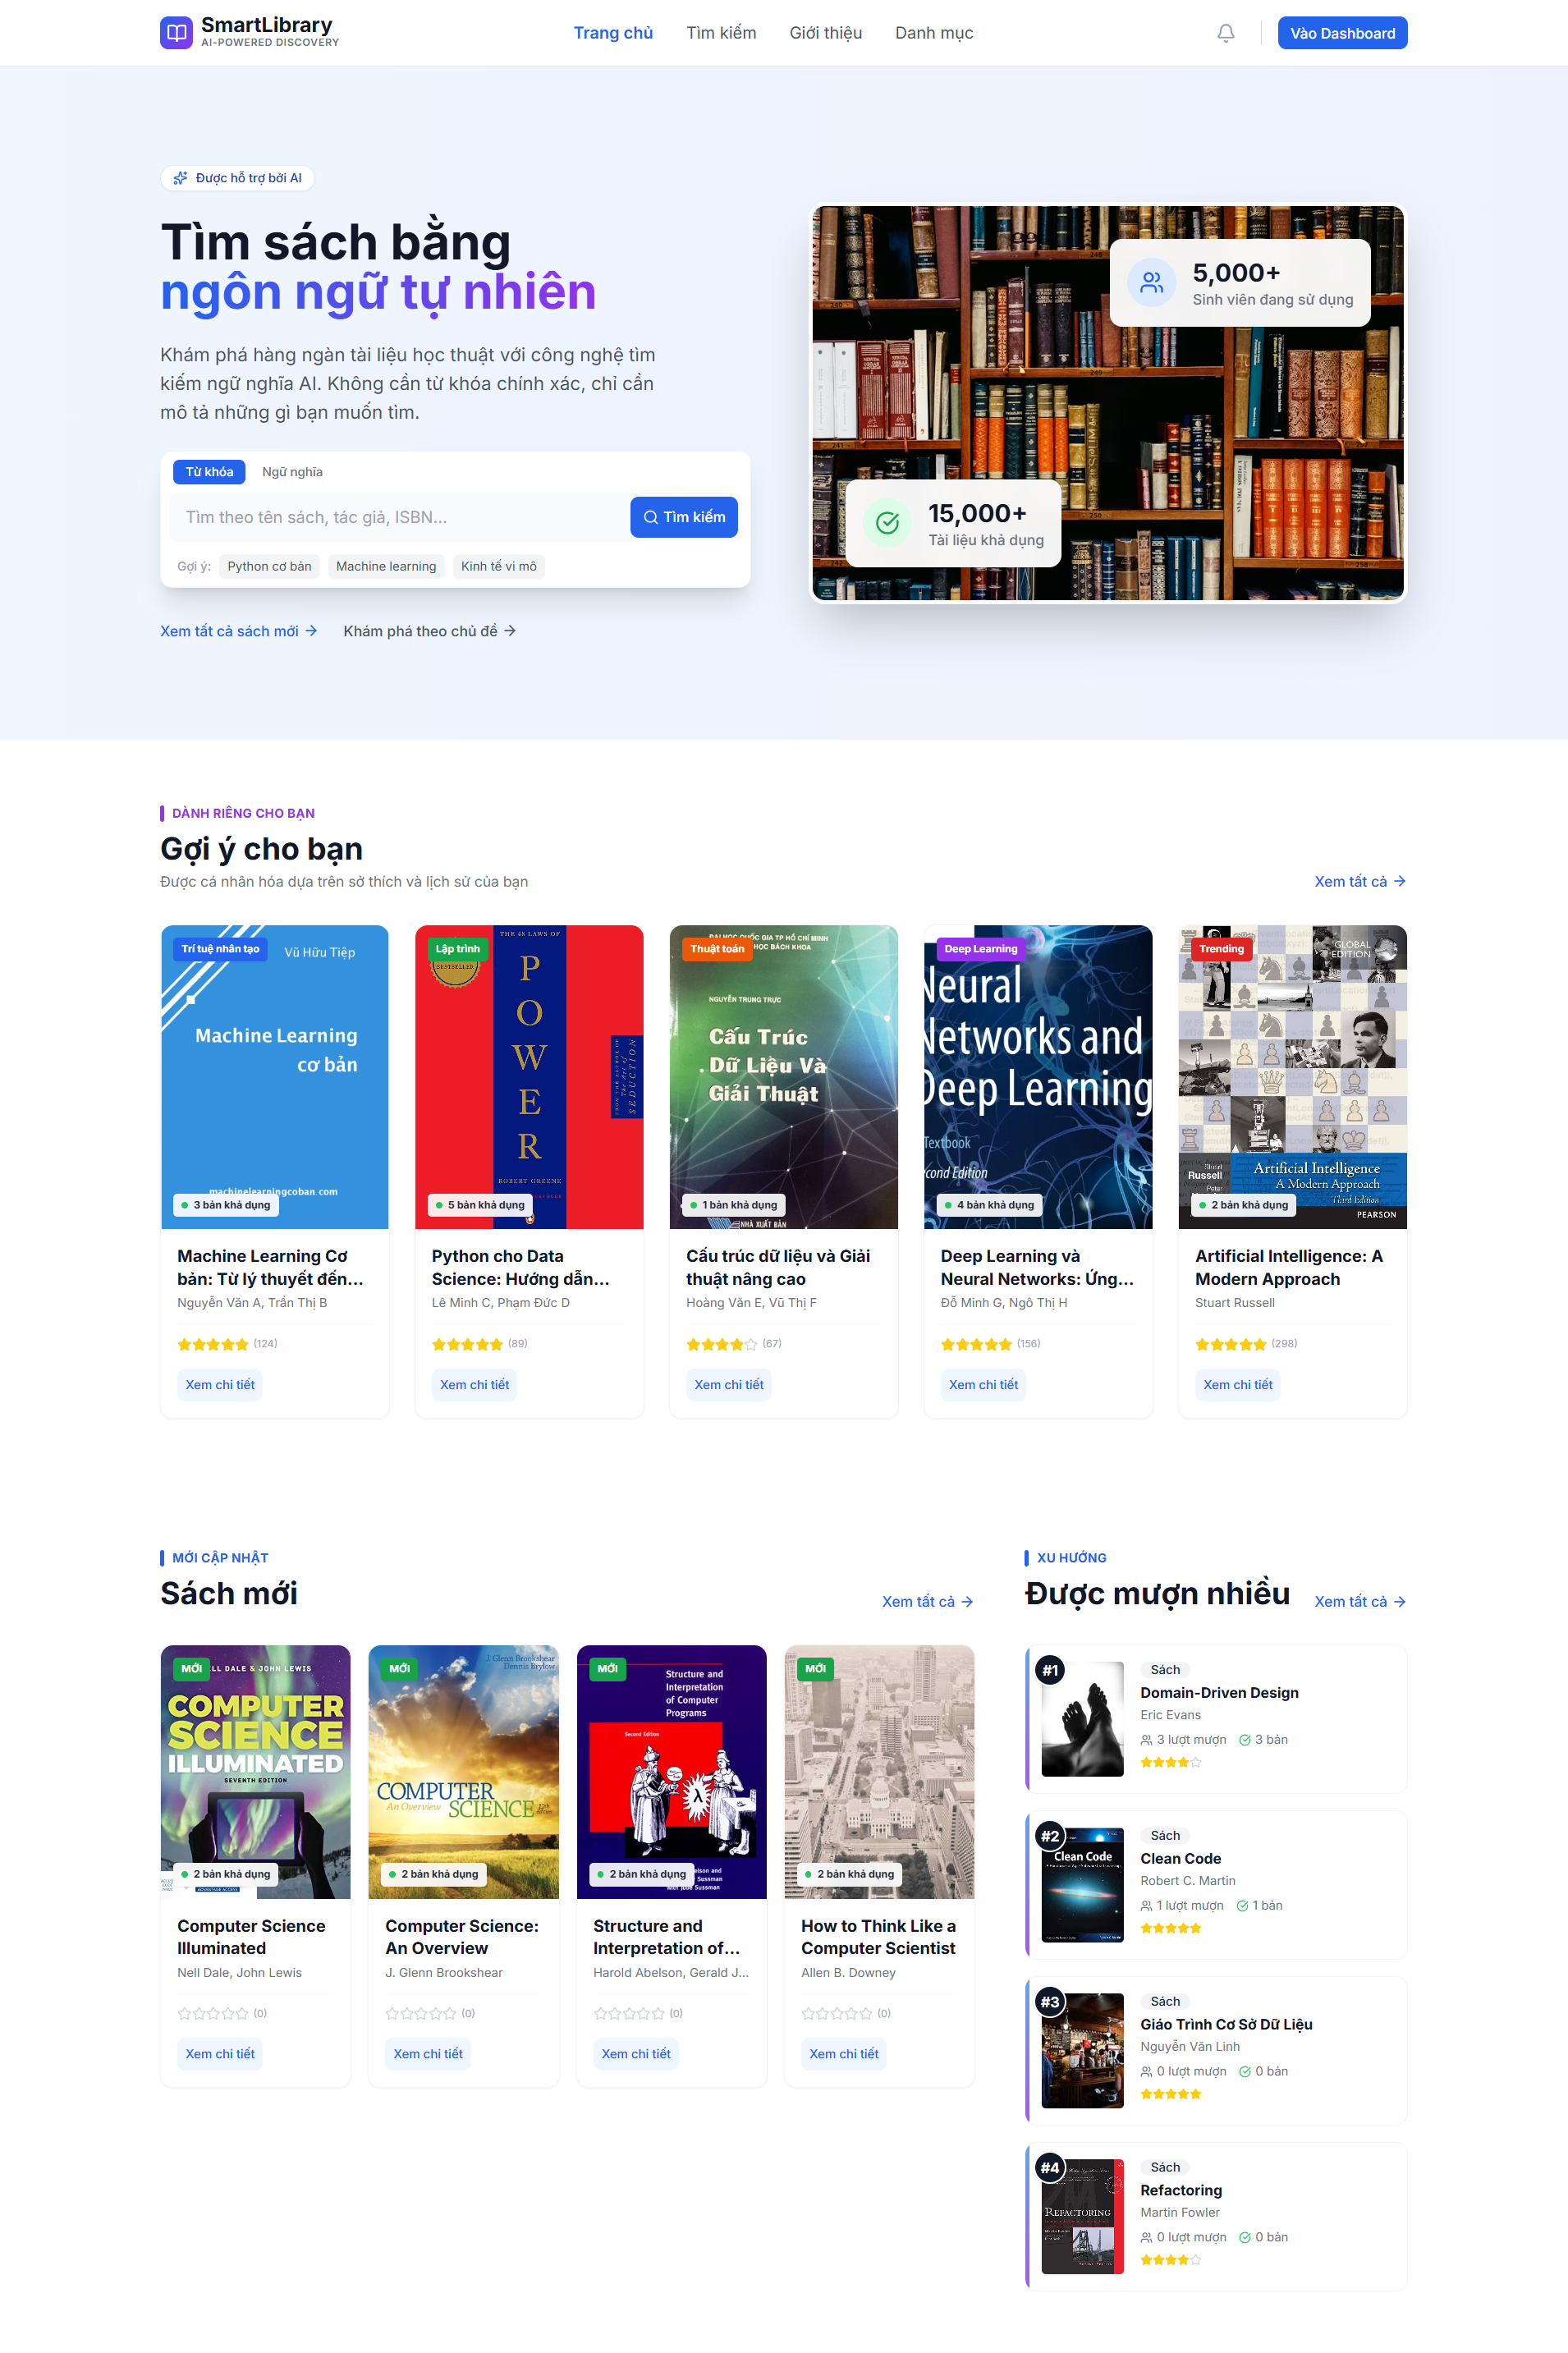
\includegraphics[width=\linewidth, height=0.38\textheight, keepaspectratio]{figures/ch05/ui/public/homepage.png}
        \caption{Trang chủ}
        \label{fig:home_page}
    \end{subfigure}
    \hfill
    \begin{subfigure}[t]{0.48\linewidth}
        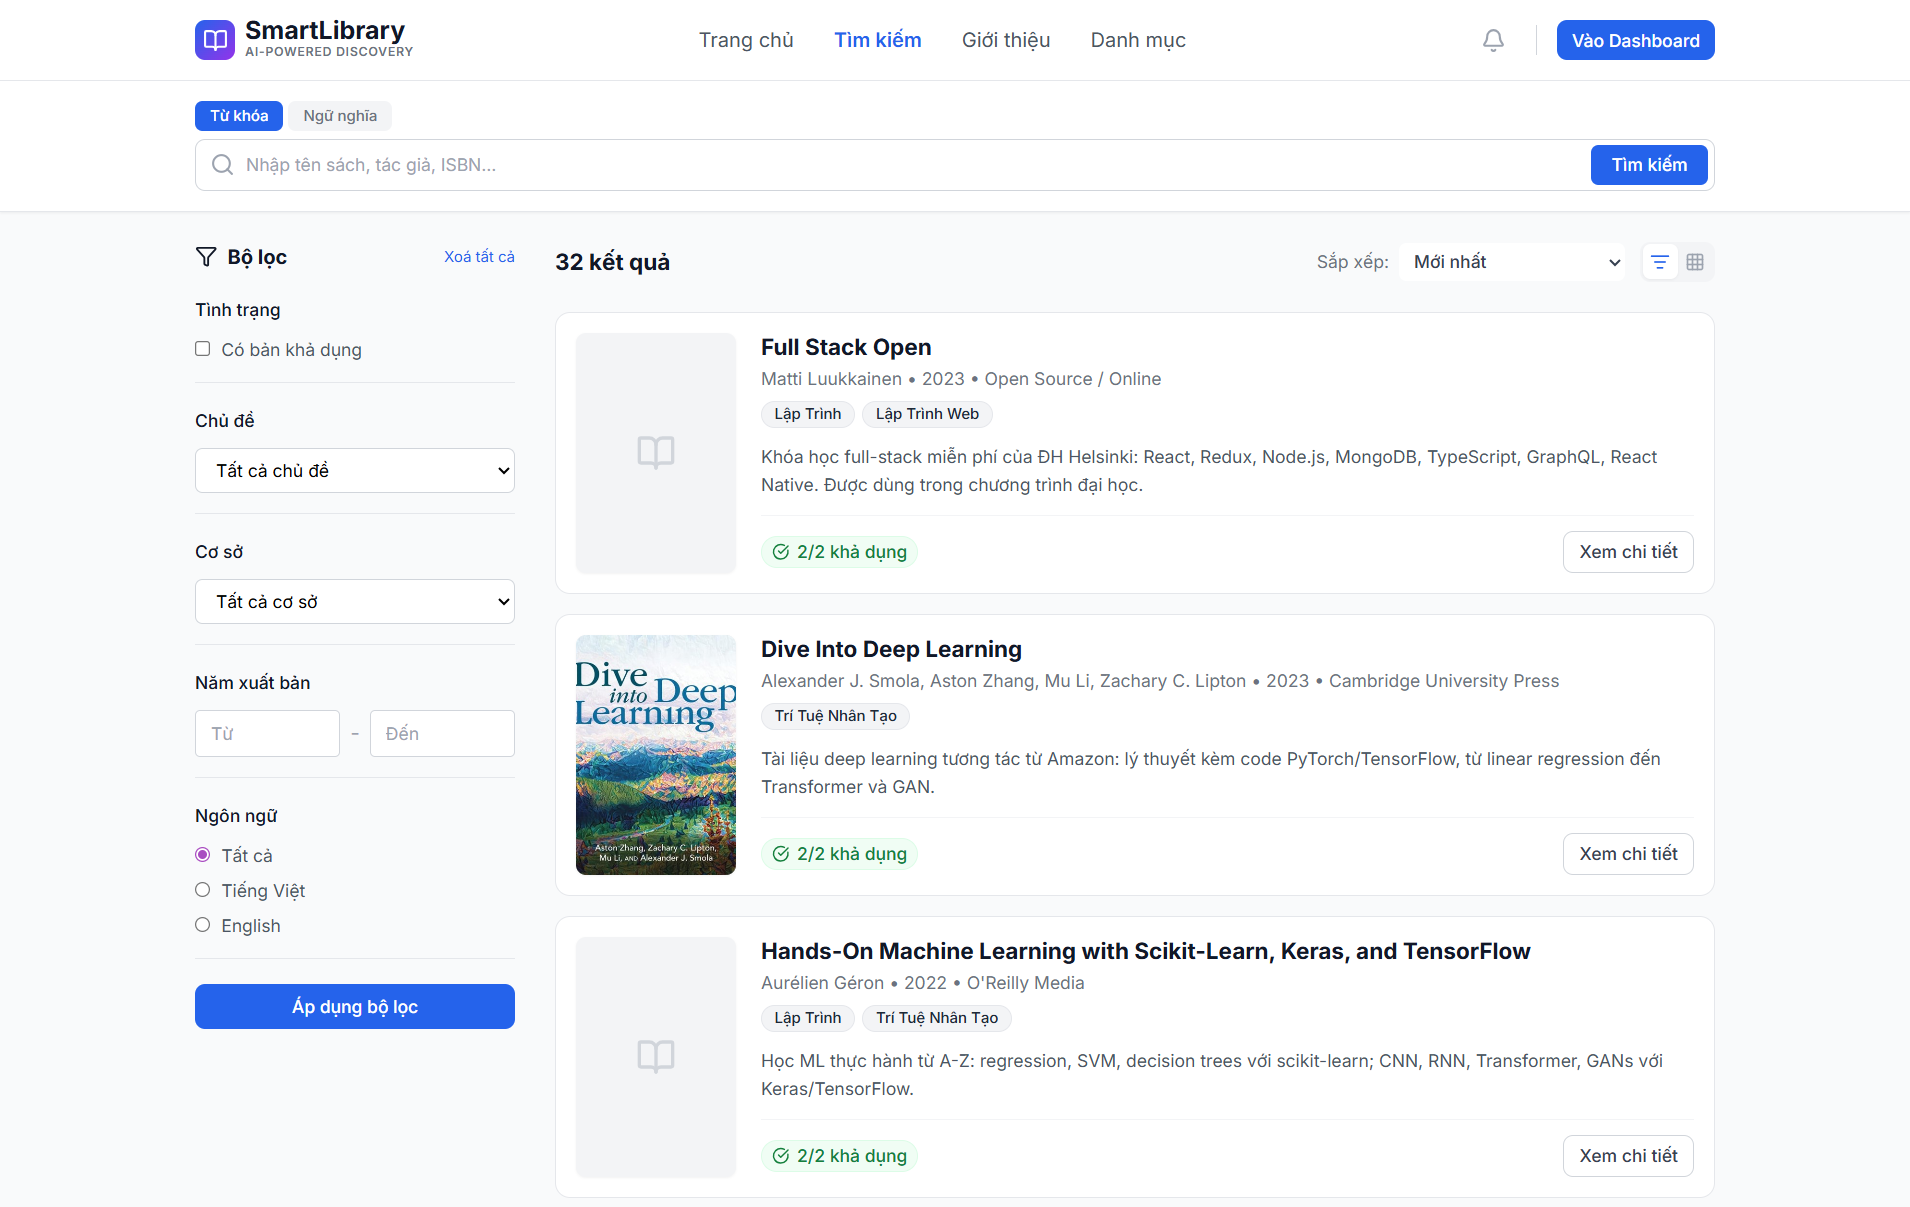
\includegraphics[width=\linewidth, height=0.38\textheight, keepaspectratio]{figures/ch05/ui/public/search_book.png}
        \caption{Tìm kiếm sách với bộ lọc}
        \label{fig:search_book}
    \end{subfigure}
    \caption{Giao diện Public: Trang chủ và Tìm kiếm}
\end{figure}


\begin{figure}[htbp]
    \centering
    
\includegraphics[width=0.6\linewidth]{figures/ch05/ui/public/book_detail.png}
    \caption{Giao diện Chi tiết sách}
    \label{fig:book_detail}
\end{figure}
\FloatBarrier

\subsubsection{Giao diện Độc giả (User Pages)}

\begin{figure}[htbp]
    \centering
    \begin{subfigure}[t]{0.48\linewidth}
        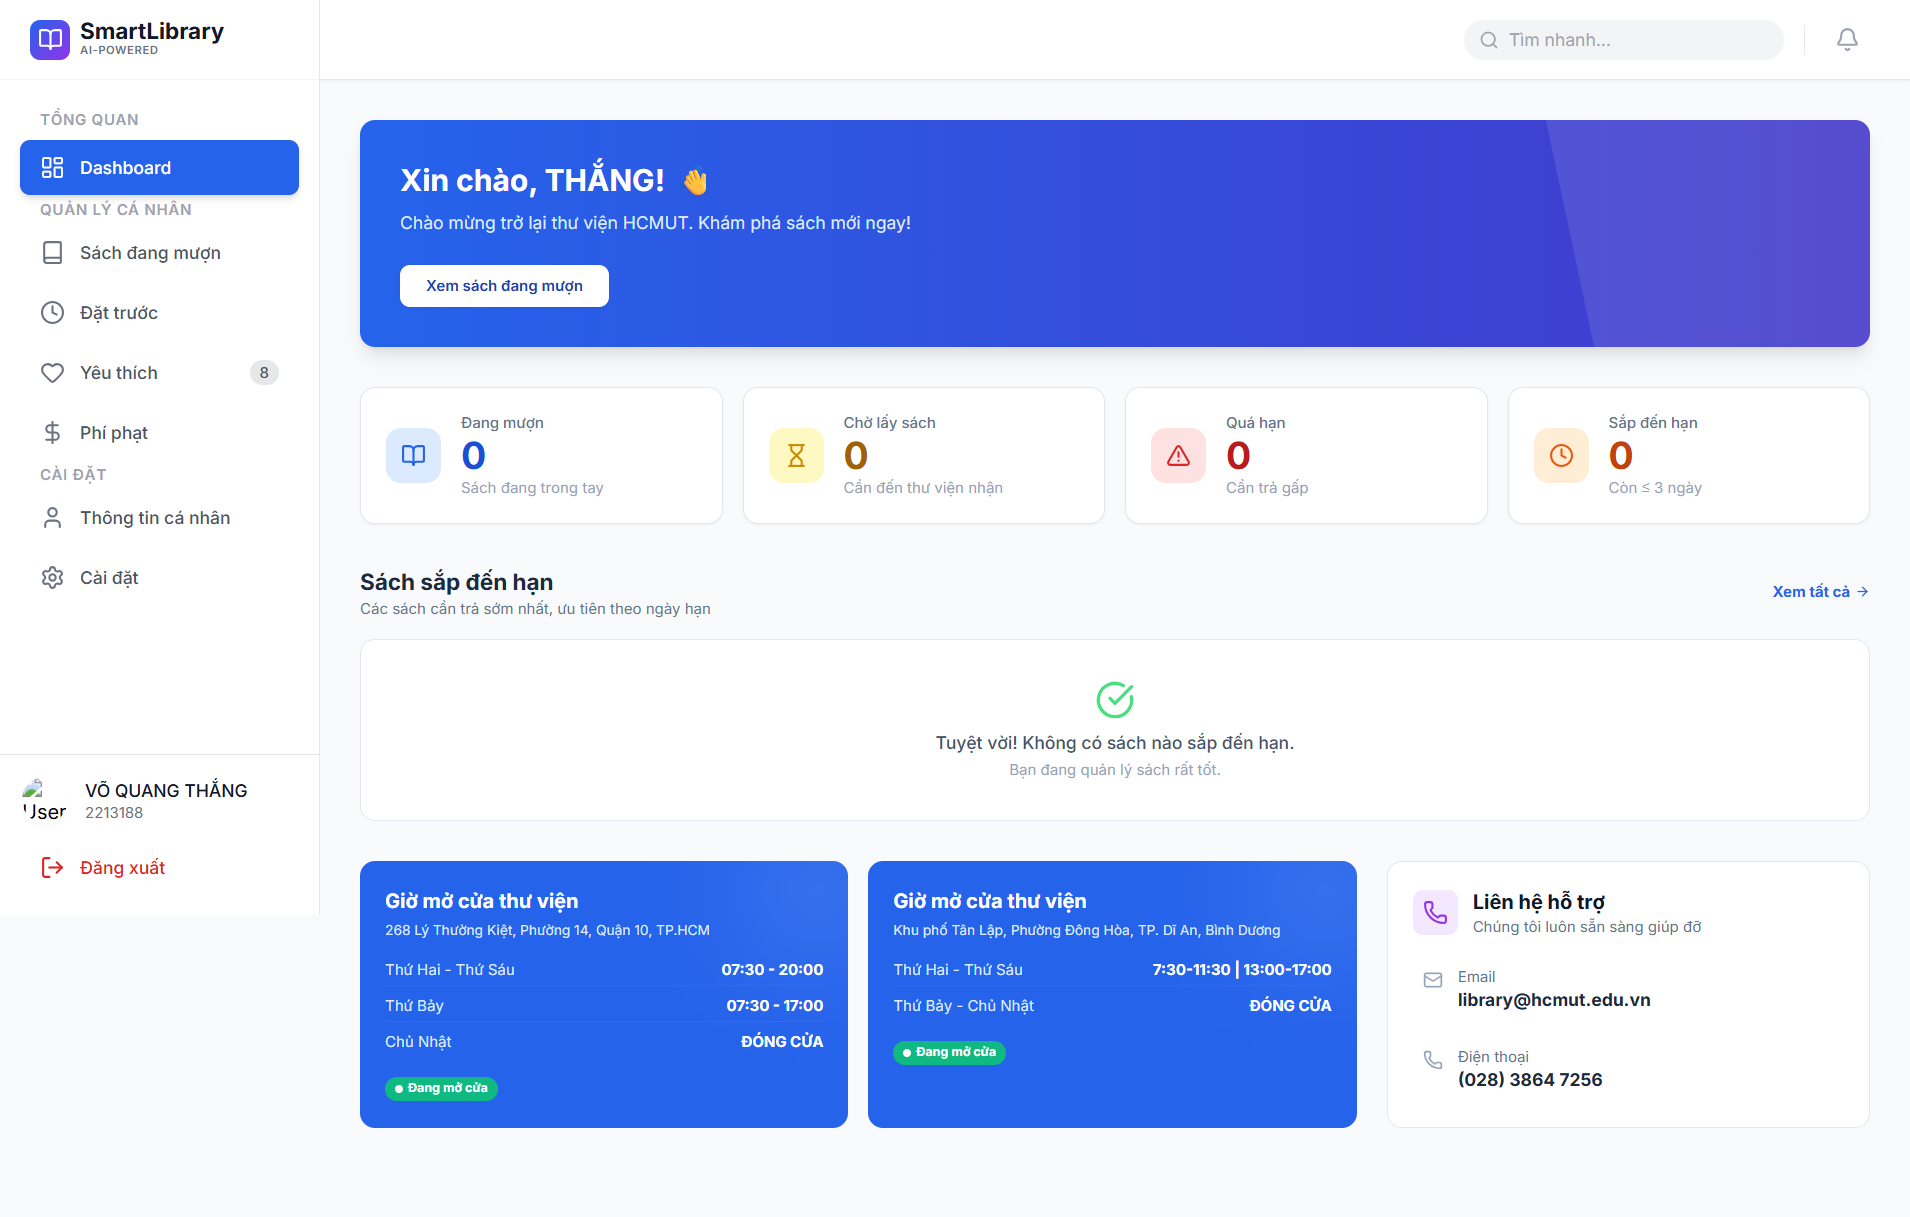
\includegraphics[width=\linewidth, height=0.38\textheight, keepaspectratio]{figures/ch05/ui/reader/dashboard.png}
        \caption{Dashboard tổng quan}
        \label{fig:user_dashboard}
    \end{subfigure}
    \hfill
    \begin{subfigure}[t]{0.48\linewidth}
        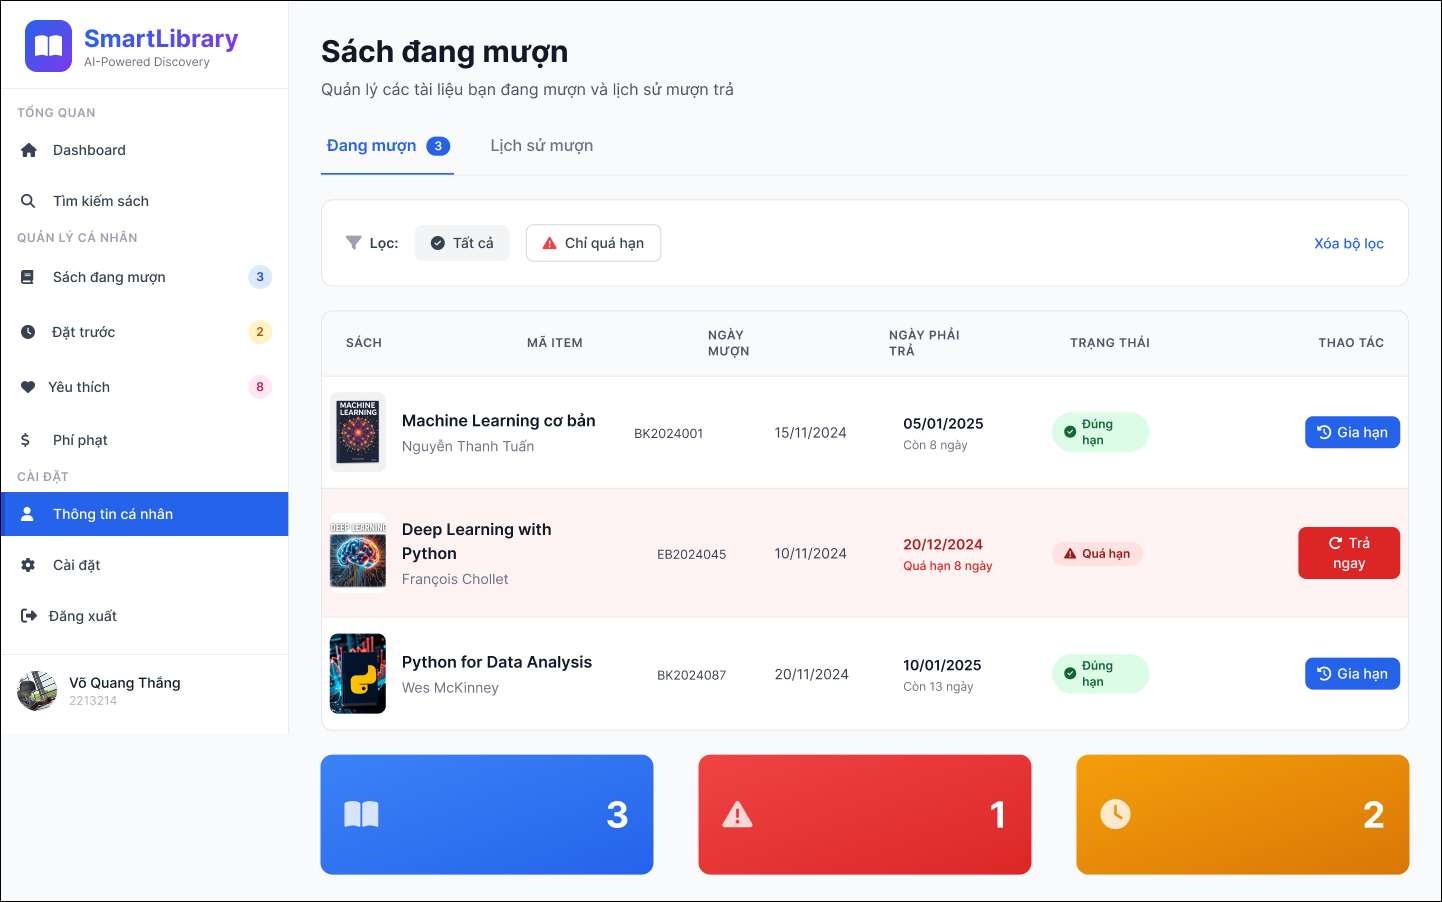
\includegraphics[width=\linewidth, height=0.38\textheight, keepaspectratio]{figures/ch05/ui/reader/current_books.png}
        \caption{Quản lý sách đang mượn}
        \label{fig:user_borrowing}
    \end{subfigure}
    \caption{Giao diện Độc giả: Dashboard và Quản lý mượn sách}
\end{figure}
\FloatBarrier

\subsubsection{Giao diện Thủ thư (Librarian Pages)}

\begin{figure}[htbp]
    \centering
    \begin{subfigure}[t]{0.48\linewidth}
        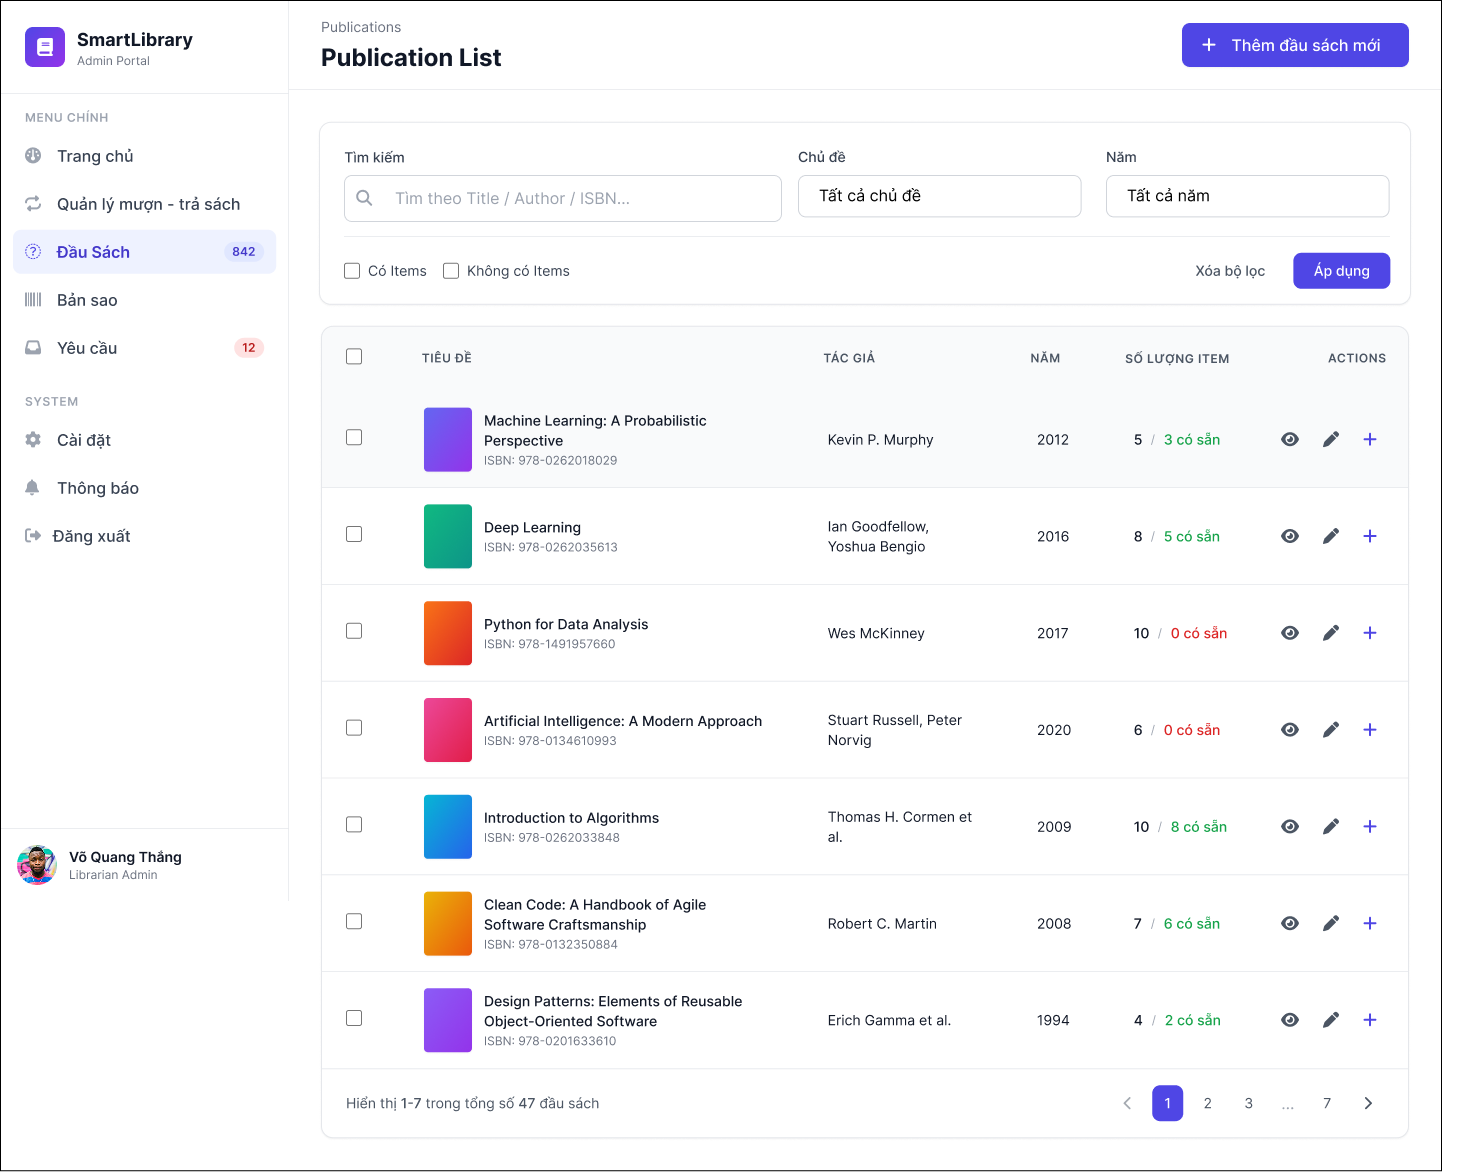
\includegraphics[width=\linewidth, height=0.38\textheight, keepaspectratio]{figures/ch05/ui/librarian/publication_list.png}
        \caption{Quản lý danh mục sách}
        \label{fig:lib_pub_list}
    \end{subfigure}
    \hfill
    \begin{subfigure}[t]{0.48\linewidth}
        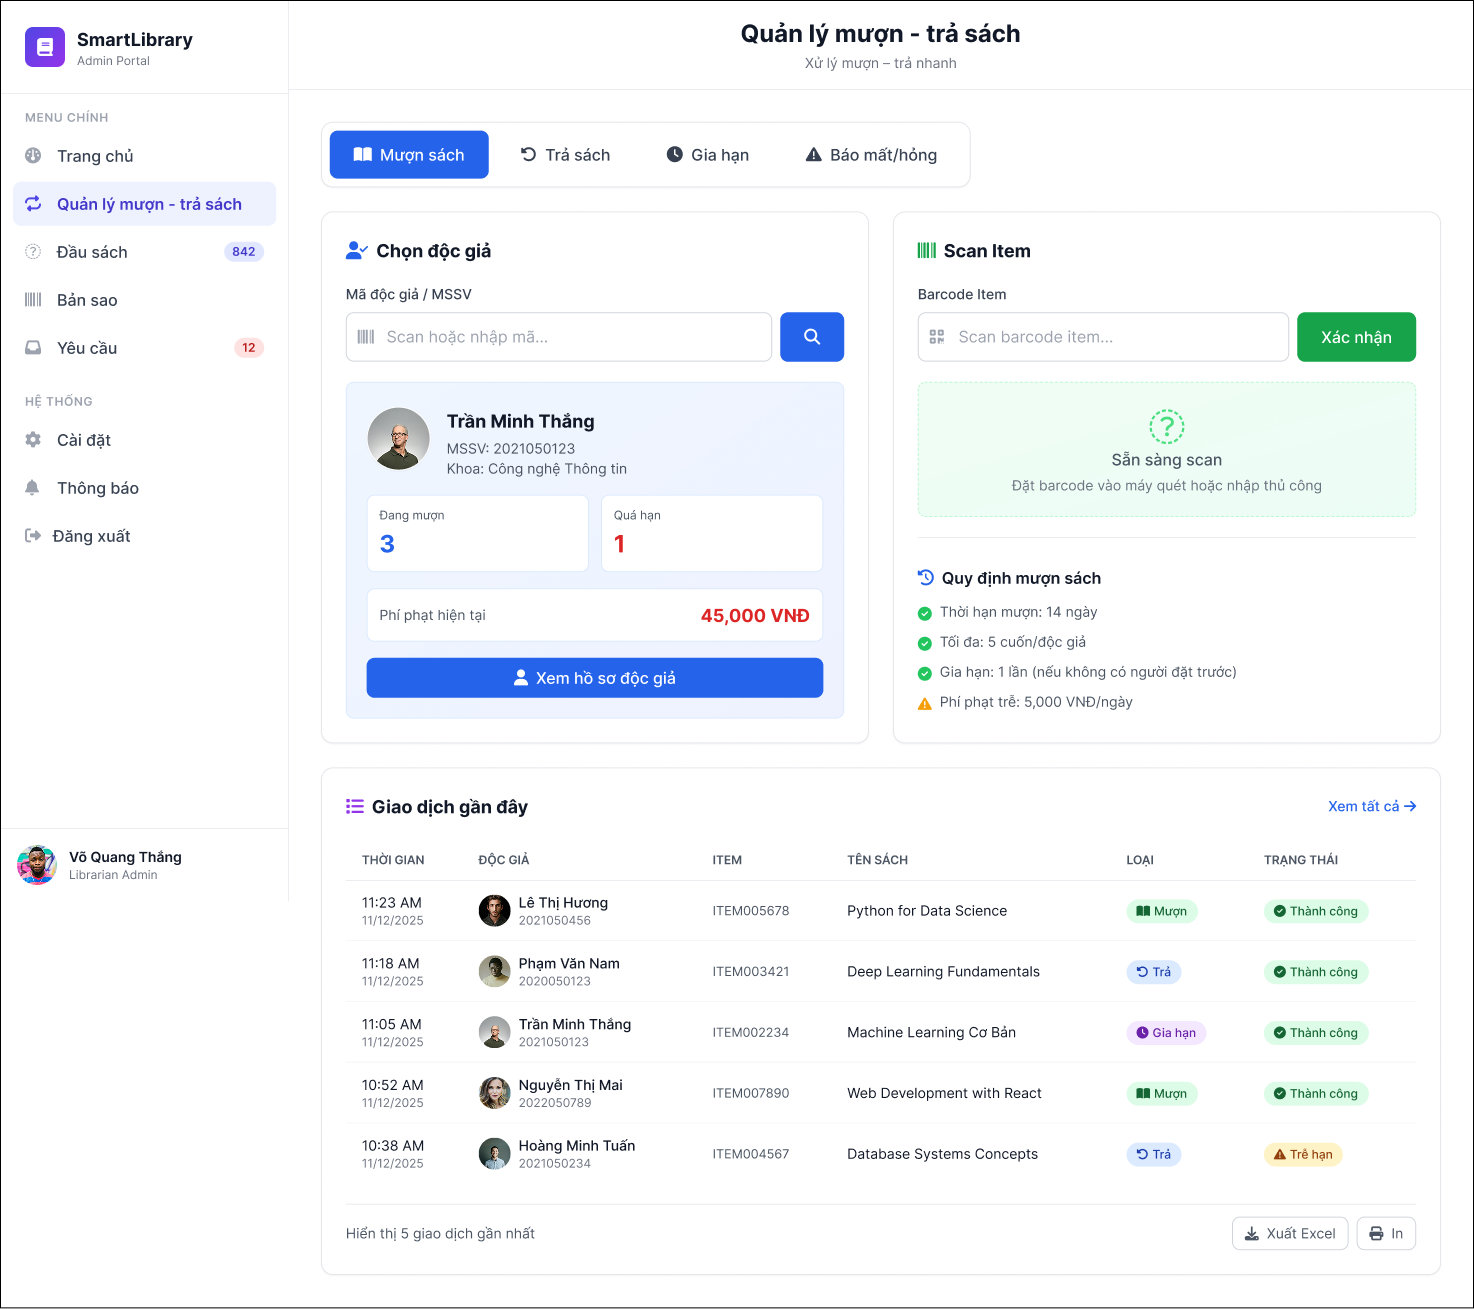
\includegraphics[width=\linewidth, height=0.38\textheight, keepaspectratio]{figures/ch05/ui/librarian/borrow_book.png}
        \caption{Ghi nhận mượn sách (Check-out)}
        \label{fig:lib_checkout}
    \end{subfigure}
    \caption{Giao diện Thủ thư: Quản lý danh mục và Lưu thông}
\end{figure}
\FloatBarrier

\chapter{Hiện thực hệ thống}

\section{Hiện thực ứng dụng}

Phần hiện thực được tổ chức theo ba lớp triển khai chính của hệ thống:
frontend, backend và AI service. Để tránh báo cáo bị dàn trải, chương này trình
bày theo dạng tổng hợp những gì nhóm đã hiện thực, thay vì mô tả tuần tự từng
màn hình hoặc từng hàm. Cách trình bày này giúp thể hiện đầy đủ phạm vi công
việc đã làm nhưng vẫn giữ báo cáo ngắn gọn.

\subsection{Hiện thực Frontend}

Nhóm đã hiện thực frontend bằng React, TypeScript và Vite theo mô hình Single
Page Application. Frontend đảm nhiệm hiển thị dữ liệu, điều phối trạng thái đăng
nhập, phân vùng giao diện theo vai trò, gọi API nghiệp vụ, nhận thông báo thời
gian thực, upload tài liệu, hiển thị QR nhận sách và hỗ trợ thanh toán phí phạt
qua PayOS. Mã nguồn được chia theo trách nhiệm: \texttt{pages} chứa màn hình
nghiệp vụ, \texttt{components} chứa thành phần tái sử dụng, \texttt{contexts}
chứa state dùng chung, \texttt{api} đóng gói HTTP service và \texttt{utils} chứa
các hàm xử lý thuần.


Để đáp ứng độ phức tạp của một hệ thống nghiệp vụ tích hợp AI và thanh toán, phân hệ Frontend được thiết kế tuân thủ nghiêm ngặt nguyên lý phân tách trách nhiệm (Separation of Concerns). Hình \ref{fig:fe_architecture_and_structure} minh họa chi tiết sơ đồ kiến trúc luồng dữ liệu (Data Flow) cùng với cấu trúc thư mục thực tế của dự án.

Cụ thể, lớp \texttt{api} được đóng gói độc lập để xử lý giao tiếp HTTP và refresh token tự động. Dữ liệu sau đó được đẩy lên lớp \texttt{contexts} để quản lý trạng thái tập trung (Global State), và cuối cùng mới được phân phối xuống các trang (\texttt{pages}) và thành phần giao diện (\texttt{components}) để hiển thị cho người dùng.

\begin{figure}[H]
    \centering
    \begin{subfigure}[b]{0.65\textwidth}
        \centering
        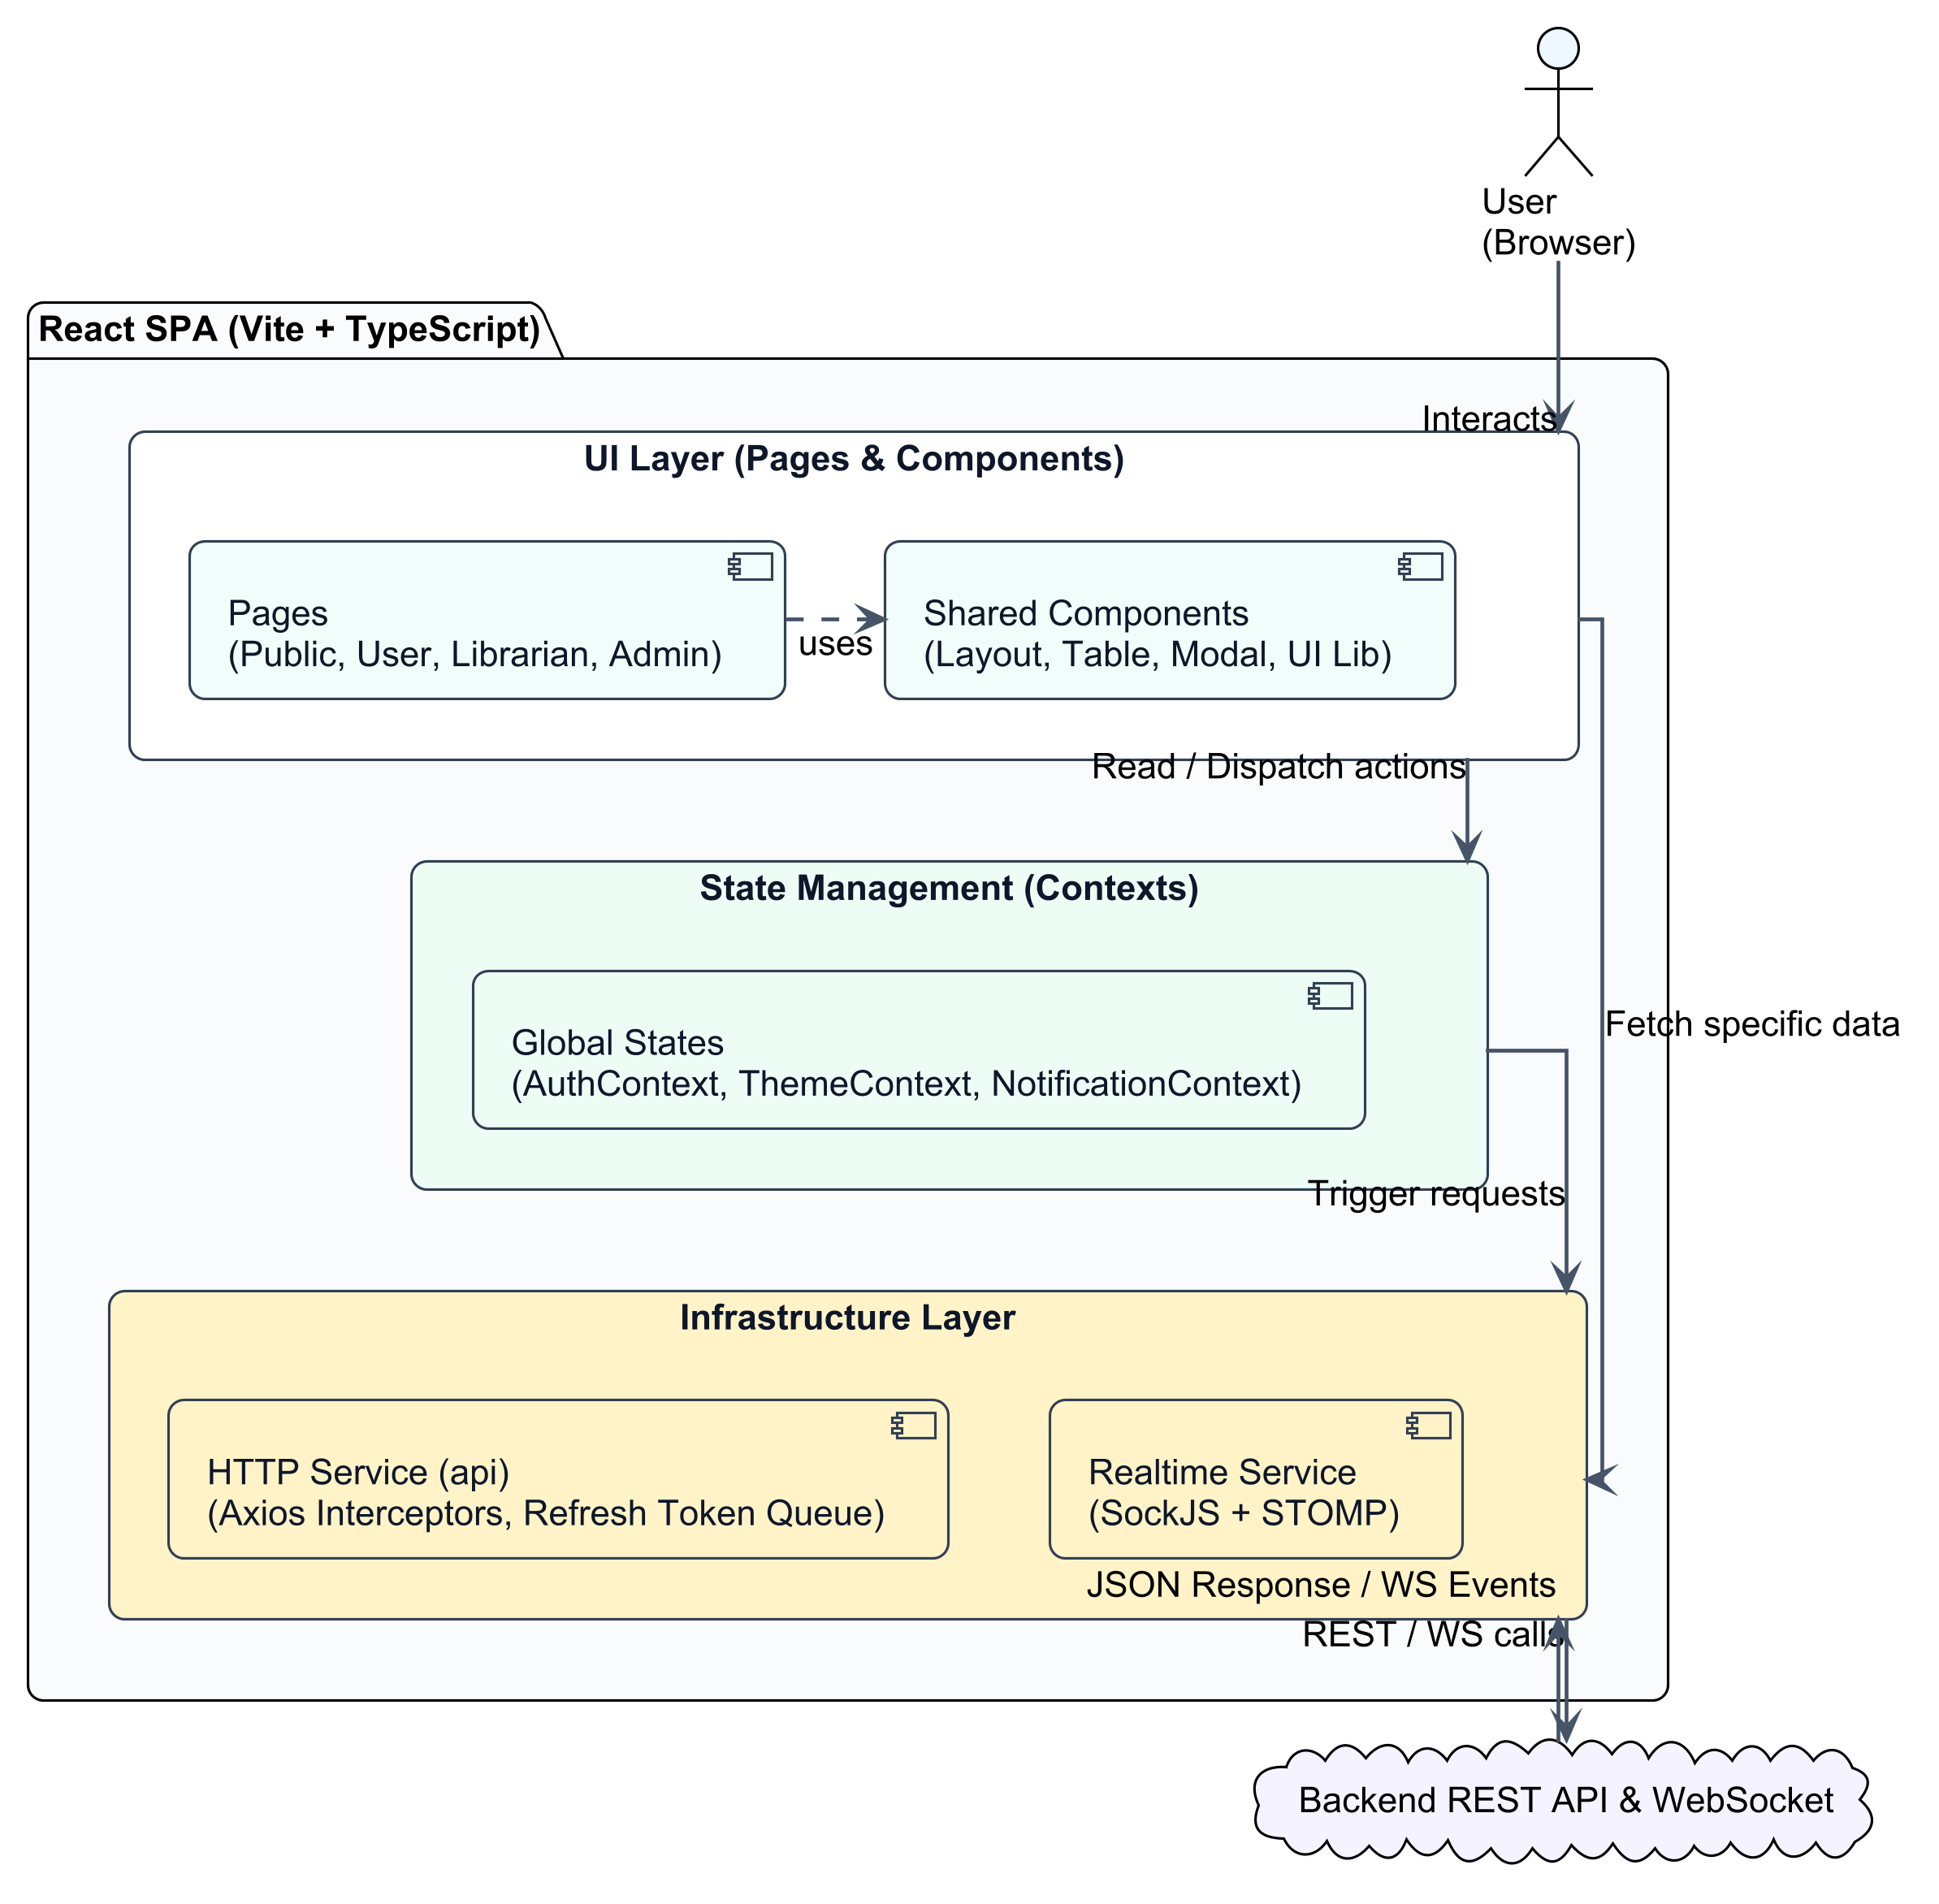
\includegraphics[width=\linewidth]{figures/ch06/frontend/frontend_architecture.png}
        \caption{Sơ đồ kiến trúc và luồng dữ liệu Frontend}
    \end{subfigure}
    \hfill
    \begin{subfigure}[b]{0.3\textwidth}
        \centering
        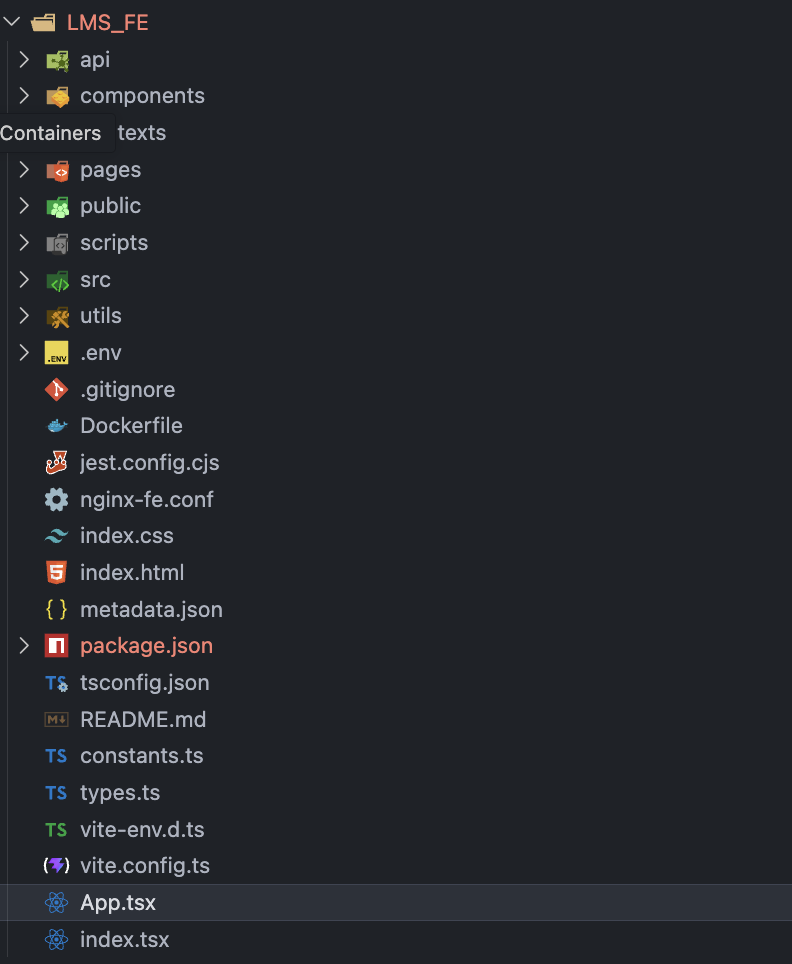
\includegraphics[width=\linewidth]{figures/ch06/frontend/frontend_folder_tree.png}
        \caption{Cấu trúc thư mục \texttt{src} thực tế}
    \end{subfigure}
    \caption{Kiến trúc tổng thể và cách thức tổ chức mã nguồn Frontend}
    \label{fig:fe_architecture_and_structure}
\end{figure}

Dựa trên nền tảng kiến trúc vững chắc này, hệ thống đã triển khai thành công các luồng nghiệp vụ phức tạp và phân định rạch ròi quyền truy cập thông qua cơ chế Route Protection. Bảng \ref{tab:fe_pages_implemented} liệt kê chi tiết danh sách các màn hình chức năng đã được hiện thực và phân quyền cụ thể cho từng nhóm người dùng (Bạn đọc, Thủ thư, Quản trị viên).

\begin{longtable}{|p{2.9cm}|p{4.2cm}|p{7.2cm}|}
\caption{Các màn hình Frontend đã hiện thực theo nhóm người dùng}
\label{tab:fe_pages_implemented}\\
\hline
\textbf{Nhóm trang} & \textbf{Màn hình} & \textbf{Chức năng đã hiện thực} \\
\hline
\endfirsthead
\hline
\textbf{Nhóm trang} & \textbf{Màn hình} & \textbf{Chức năng đã hiện thực} \\
\hline
\endhead
\texttt{/publicpage} & Trang chủ &
Hiển thị sách mới, sách được mượn nhiều, sách được đánh giá cao, thống kê công
khai và ô tìm kiếm nhanh. \\
\hline
\texttt{/publicpage} & Tìm kiếm sách &
Tìm kiếm theo từ khóa, lọc danh mục/tag/ngôn ngữ/năm xuất bản/trạng thái bản
sao, sắp xếp, phân trang và chuyển sang semantic search khi cần. \\
\hline
\texttt{/publicpage} & Chi tiết sách &
Hiển thị metadata, bản sao, trạng thái khả dụng, summary/tag AI, rating, review,
sách tương tự, nút mượn hoặc đặt trước. \\
\hline
\texttt{/publicpage} & Auth pages &
Đăng ký, đăng nhập, Google OAuth callback, xác thực email, quên mật khẩu và đặt
lại mật khẩu. \\
\hline
\texttt{/publicpage} & Liên hệ, hướng dẫn, FAQ &
Hiển thị thông tin thư viện, form liên hệ, iframe Google Maps lazy loading và
nội dung hướng dẫn sử dụng. \\
\hline
\texttt{/userpage} & Dashboard bạn đọc &
Tổng hợp sách đang mượn, đặt trước, phí phạt, thông báo, gợi ý sách và thao tác
nhanh. \\
\hline
\texttt{/userpage} & Sách đang mượn/lịch sử &
Theo dõi giao dịch mượn, hạn trả, trạng thái quá hạn, lịch sử mượn trả và chi
tiết giao dịch. \\
\hline
\texttt{/userpage} & Đặt trước &
Xem danh sách phiếu đặt trước, vị trí hàng chờ, trạng thái sẵn sàng nhận sách,
deadline và hủy đặt trước. \\
\hline
\texttt{/userpage} & Phí phạt &
Xem phí quá hạn/hư/mất, trạng thái thanh toán, tạo QR PayOS và cập nhật kết quả
thanh toán. \\
\hline
\texttt{/userpage} & Wishlist, rating, hồ sơ &
Lưu sách yêu thích, đánh giá sách sau khi mượn, phản hồi review, cập nhật hồ sơ,
avatar, mật khẩu, ngôn ngữ và theme. \\
\hline
\texttt{/userpage} & Thông báo &
Nhận thông báo realtime, đánh dấu đã đọc, xem thông báo về mượn--trả, đặt trước,
phí phạt và phản hồi review. \\
\hline
\texttt{/librarianpage} & Dashboard thủ thư &
Thống kê vận hành, sách mượn/trả, yêu cầu chờ xử lý, phí phạt, cảnh báo quá hạn
và các thao tác nhanh. \\
\hline
\texttt{/librarianpage} & Quản lý ấn phẩm &
Tạo/sửa/xóa ấn phẩm, tác giả, nhà xuất bản, danh mục, tag, ảnh bìa, ISBN auto
fill, upload PDF và theo dõi trạng thái xử lý AI. \\
\hline
\texttt{/librarianpage} & Quản lý bản sao &
Tạo bản sao vật lý, barcode, vị trí kệ, chi nhánh, trạng thái khả dụng, hư/mất
và lịch sử lưu thông. \\
\hline
\texttt{/librarianpage} & Mượn--trả tại quầy &
Tra cứu bạn đọc, quét/nhập barcode, cho mượn trực tiếp, xác nhận nhận sách, trả
sách, ghi chú giao dịch và xử lý sách hư/mất. \\
\hline
\texttt{/librarianpage} & Yêu cầu và đặt trước &
Xem yêu cầu mượn, duyệt/từ chối, quản lý hàng chờ đặt trước, xác nhận nhận sách
và gửi thông báo cho bạn đọc. \\
\hline
\texttt{/librarianpage} & Phí phạt và thanh toán &
Tính phí, thu tiền mặt, tạo QR PayOS, polling trạng thái chuyển khoản và cập
nhật trạng thái fine. \\
\hline
\texttt{/adminpage} & Quản lý tài khoản &
Quản lý tài khoản độc giả/thủ thư, tạo thủ thư, khóa/mở khóa, xác minh tài
khoản và cập nhật trạng thái người dùng. \\
\hline
\texttt{/adminpage} & Chính sách và audit &
Cấu hình quy định mượn trả, xem nhật ký thao tác, lọc audit log và theo dõi thay
đổi vận hành hệ thống. \\
\hline
\end{longtable}

% ==========================================
% 1. PHÂN HỆ BẠN ĐỌC (READER FLOW)
% ==========================================
Để mang lại trải nghiệm liền mạch cho bạn đọc, phân hệ Frontend được thiết kế tối ưu từ khâu khám phá tài liệu đến các thao tác tương tác chi tiết. Quá trình này bắt đầu tại màn hình Dashboard và công cụ tìm kiếm ngữ nghĩa, nơi người dùng có thể tra cứu ấn phẩm bằng ngôn ngữ tự nhiên thay vì chỉ dựa vào từ khóa rập khuôn.

\begin{figure}[H]
    \centering
    \begin{subfigure}[b]{0.48\textwidth}
        \centering
        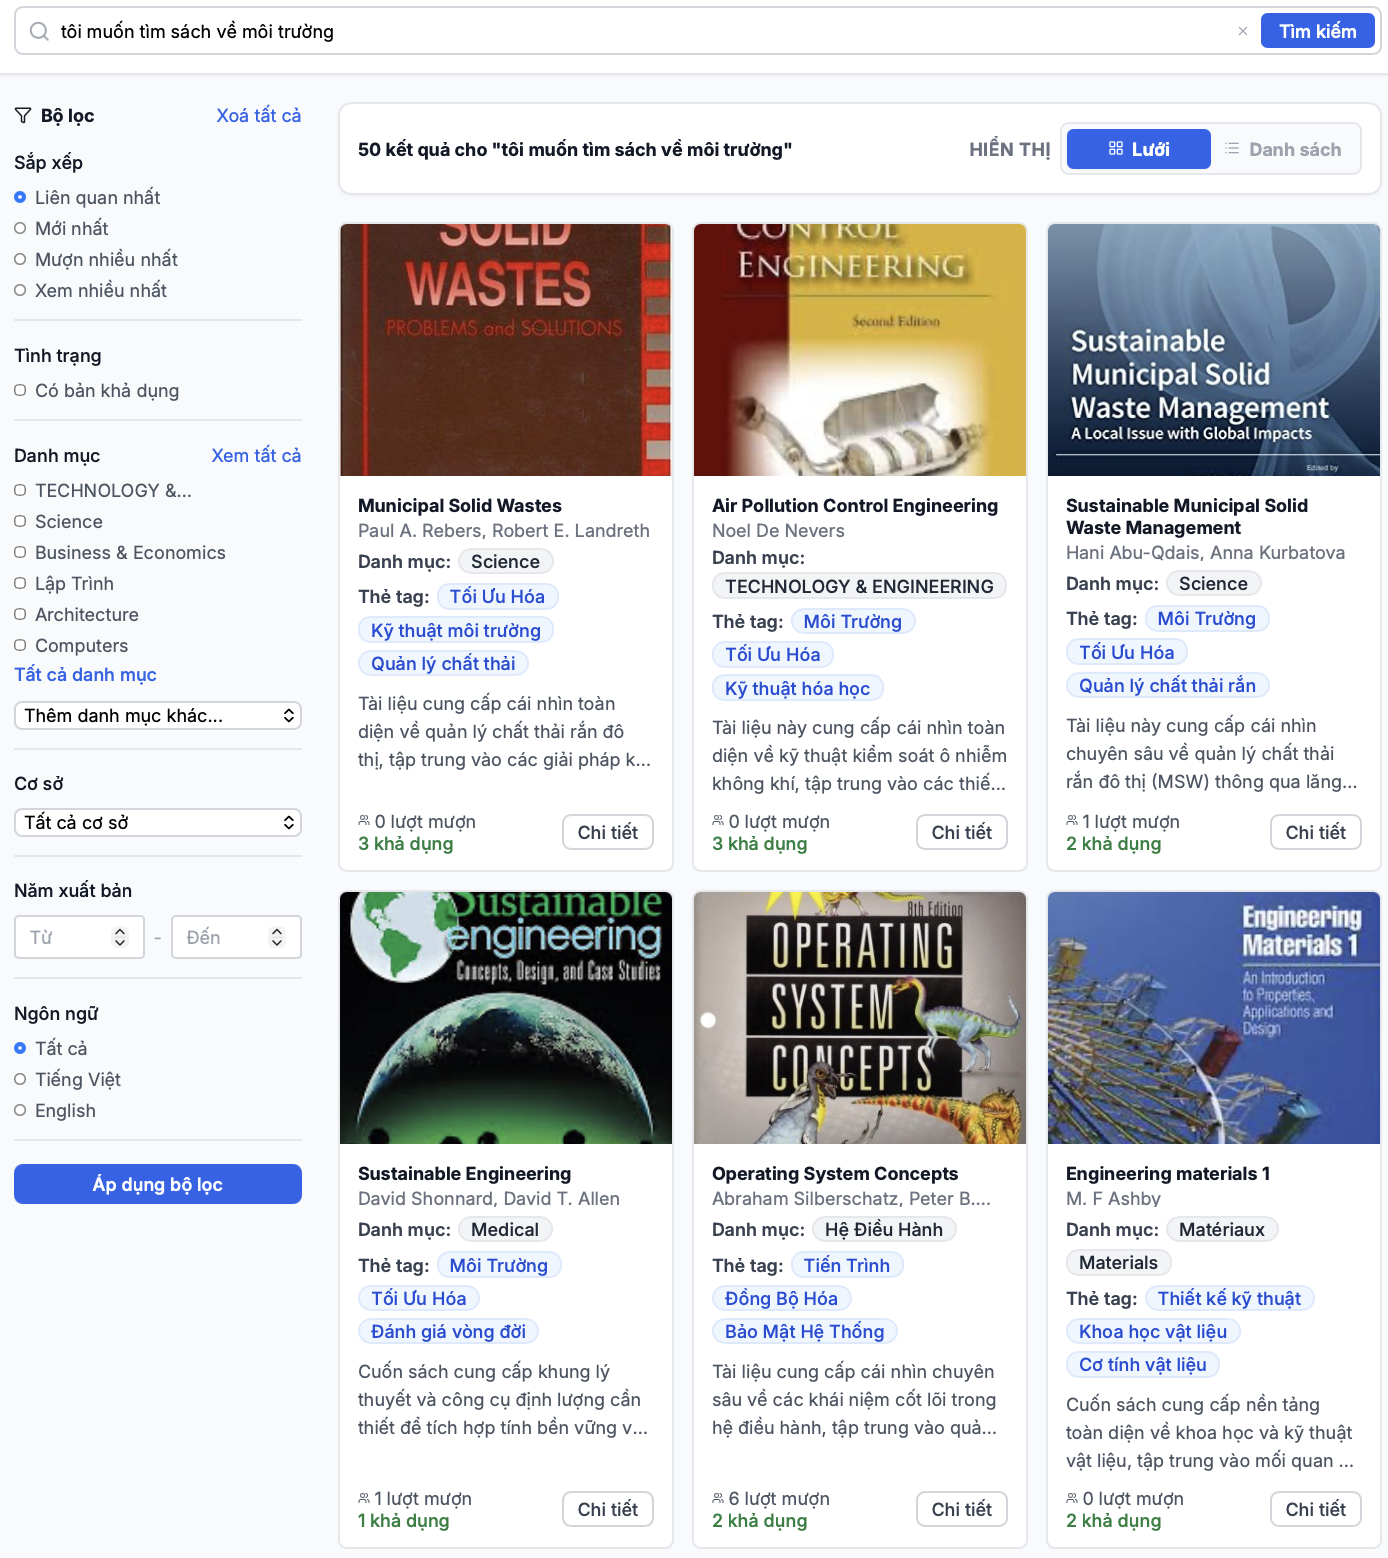
\includegraphics[width=\linewidth]{figures/ch06/frontend/semantic_search_page.png}
        \caption{Tìm kiếm ngữ nghĩa và lọc sách}
    \end{subfigure}
    \hfill
    \begin{subfigure}[b]{0.48\textwidth}
        \centering
        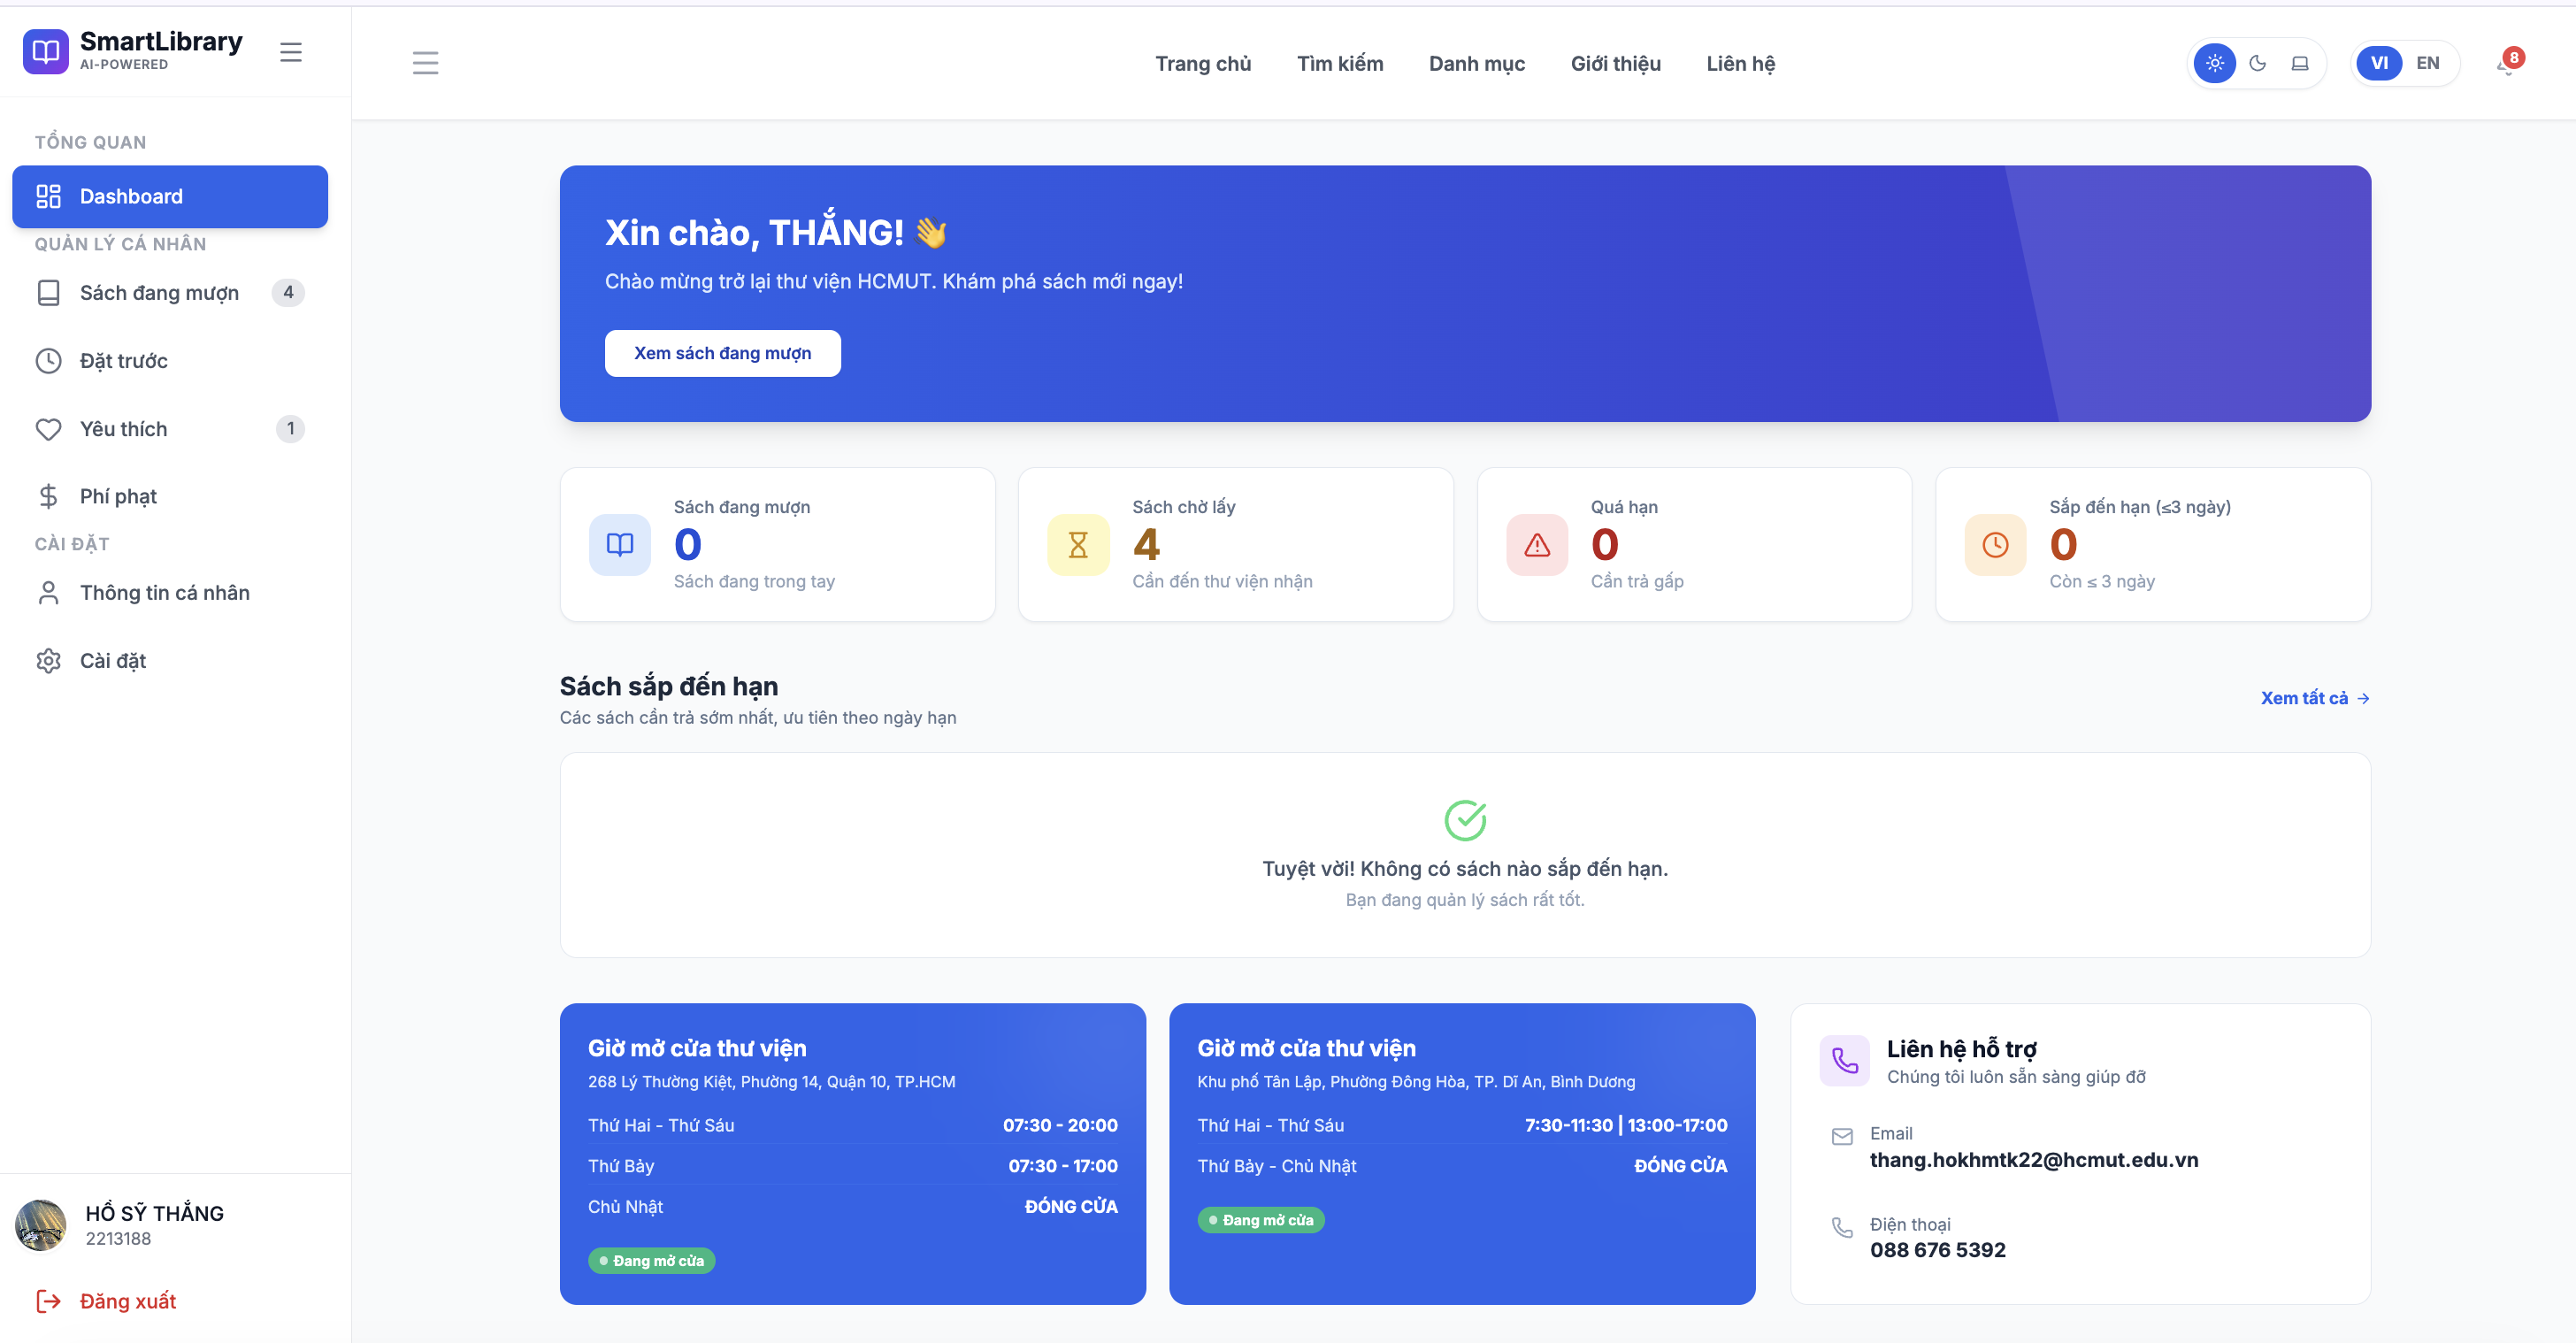
\includegraphics[width=\linewidth]{figures/ch06/frontend/reader_dashboard.png}
        \caption{Dashboard bạn đọc}
    \end{subfigure}
    \caption{Giao diện tổng quan và chức năng tìm kiếm thông minh dành cho bạn đọc}
    \label{fig:fe_reader_discovery}
\end{figure}

Sau khi tìm được tài liệu mong muốn, bạn đọc có thể xem thông tin chi tiết với các siêu dữ liệu (metadata) được AI tự động trích xuất. Đồng thời, hệ thống cung cấp đầy đủ các tính năng tương tác như đánh giá, phản hồi và thanh toán trực tuyến tự động thông qua mã QR PayOS.

\begin{figure}[H]
    \centering
    \begin{subfigure}[b]{0.48\textwidth}
        \centering
        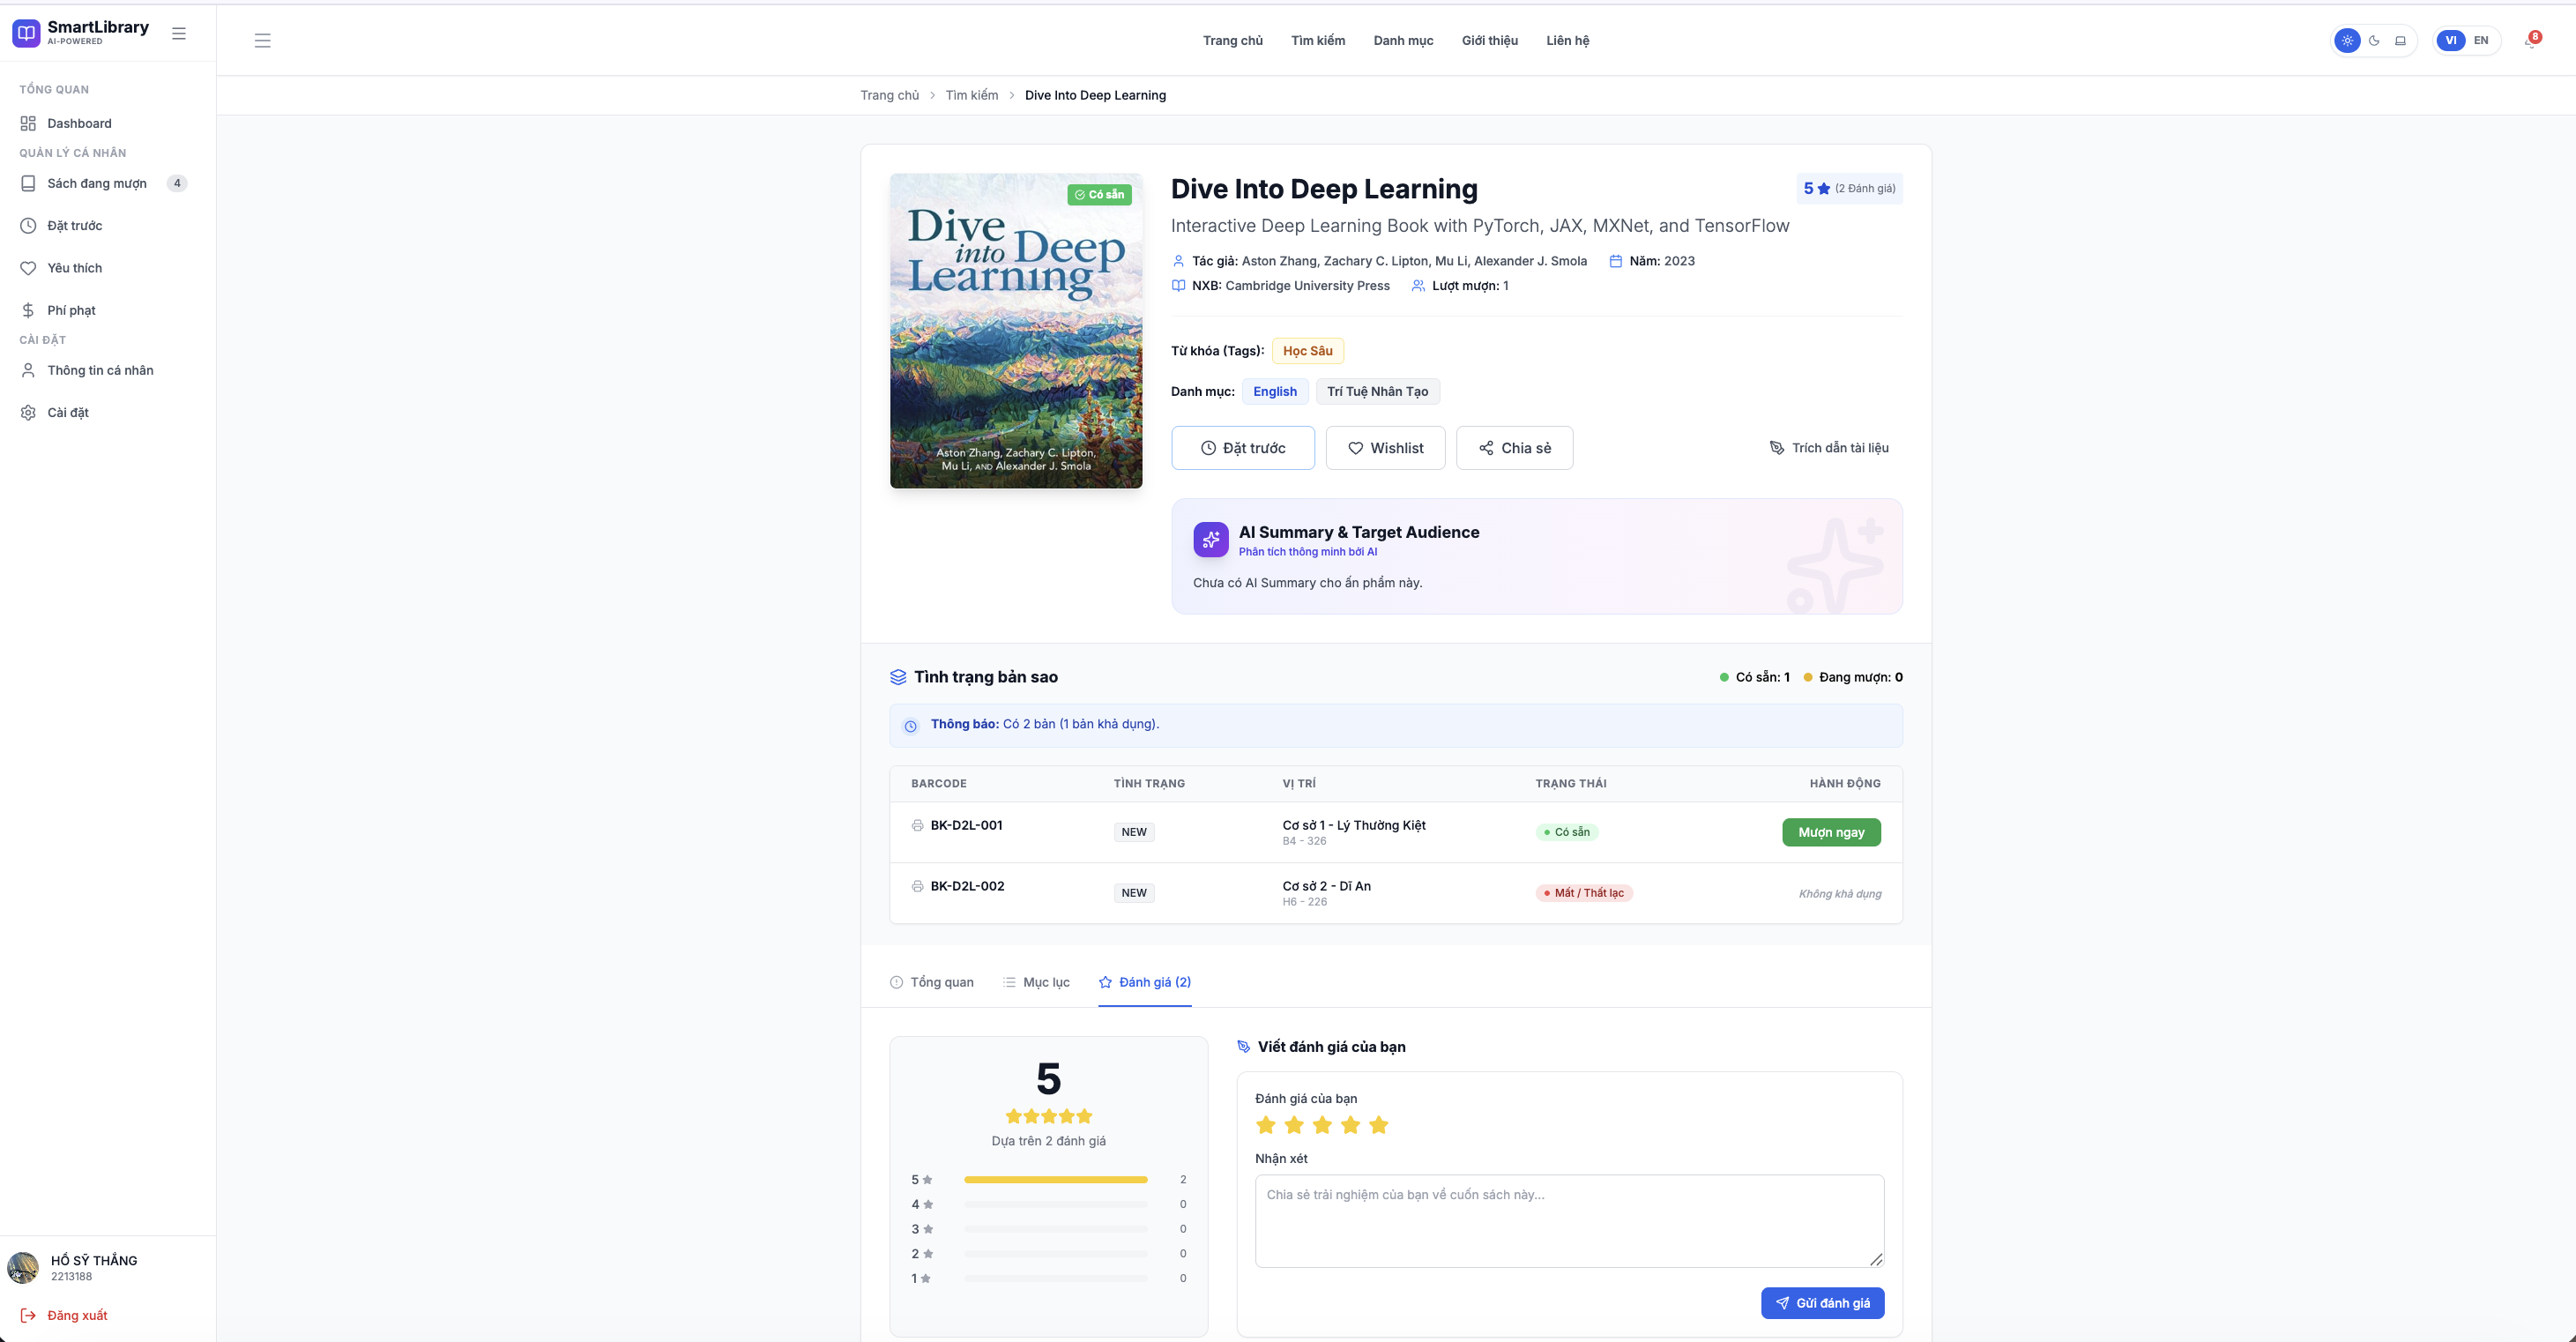
\includegraphics[width=\linewidth]{figures/ch06/frontend/book_detail.png}
        \caption{Chi tiết sách và siêu dữ liệu (metadata) AI}
    \end{subfigure}
    \hfill
    \begin{subfigure}[b]{0.48\textwidth}
        \centering
        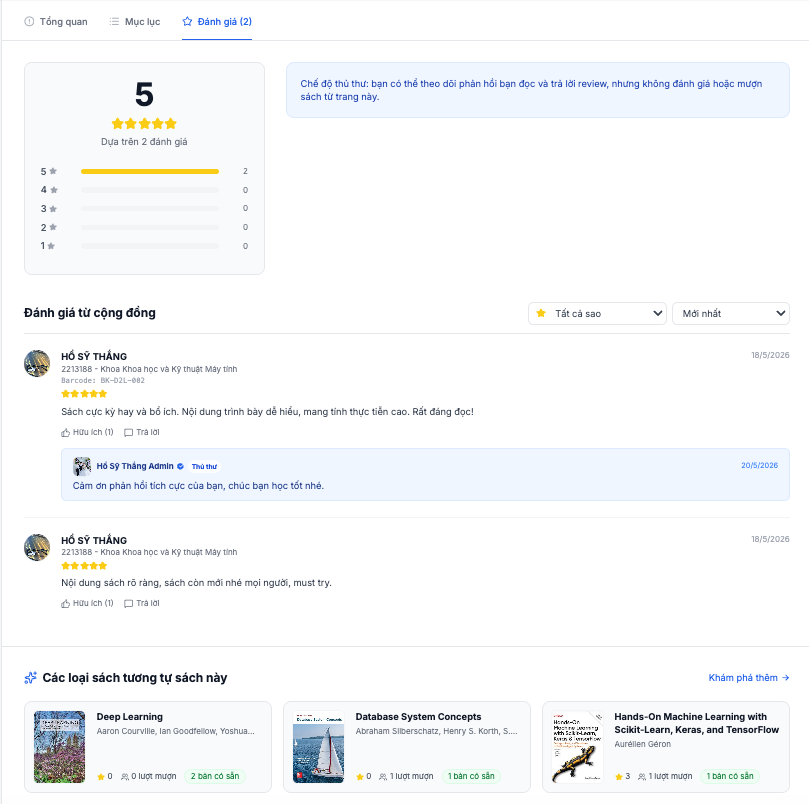
\includegraphics[width=\linewidth]{figures/ch06/frontend/book_rating_review.png}
        \caption{Đánh giá và phản hồi}
    \end{subfigure}
    \caption{Trải nghiệm xem chi tiết và tương tác với ấn phẩm}
    \label{fig:fe_reader_interaction}
\end{figure}

\begin{figure}[H]
    \centering
    \begin{subfigure}[b]{0.48\textwidth}
        \centering
        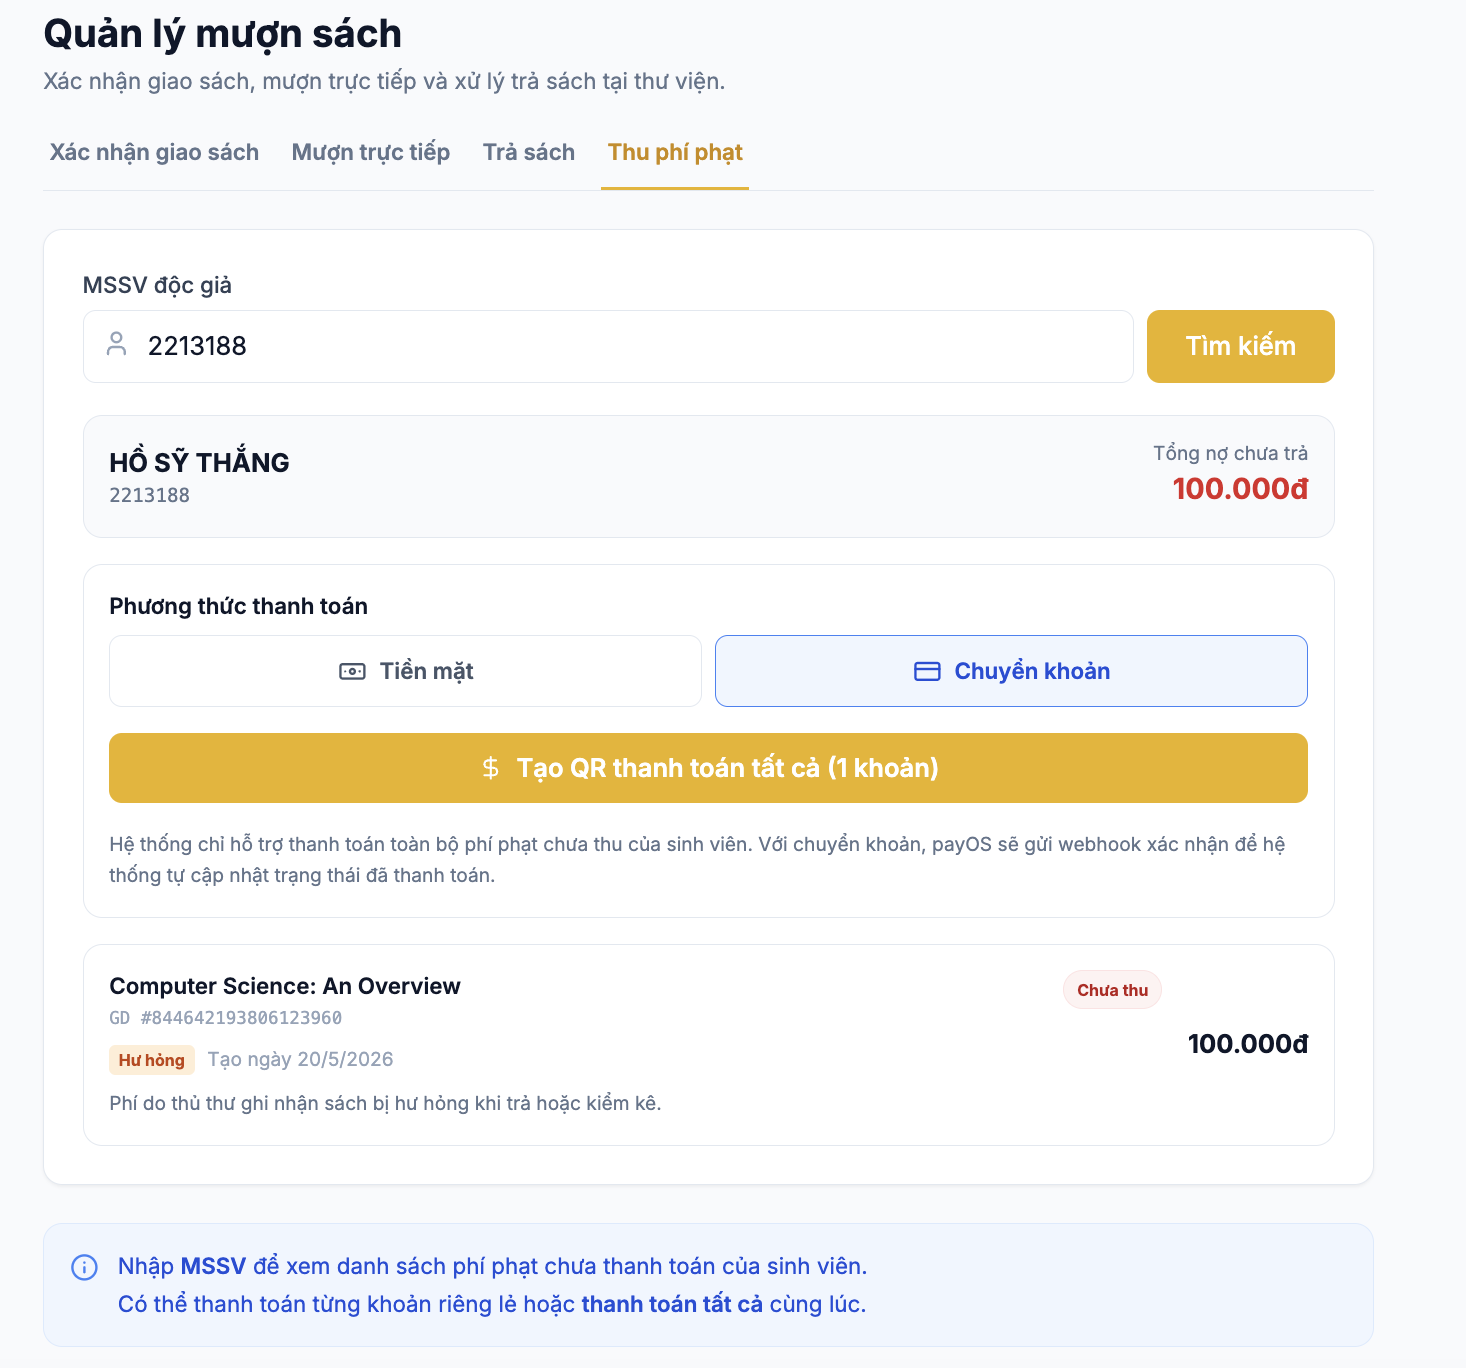
\includegraphics[width=\linewidth]{figures/ch06/payment/init_qr.png}
        \caption{Khởi tạo thanh toán}
    \end{subfigure}
    \hfill
    \begin{subfigure}[b]{0.48\textwidth}
        \centering
        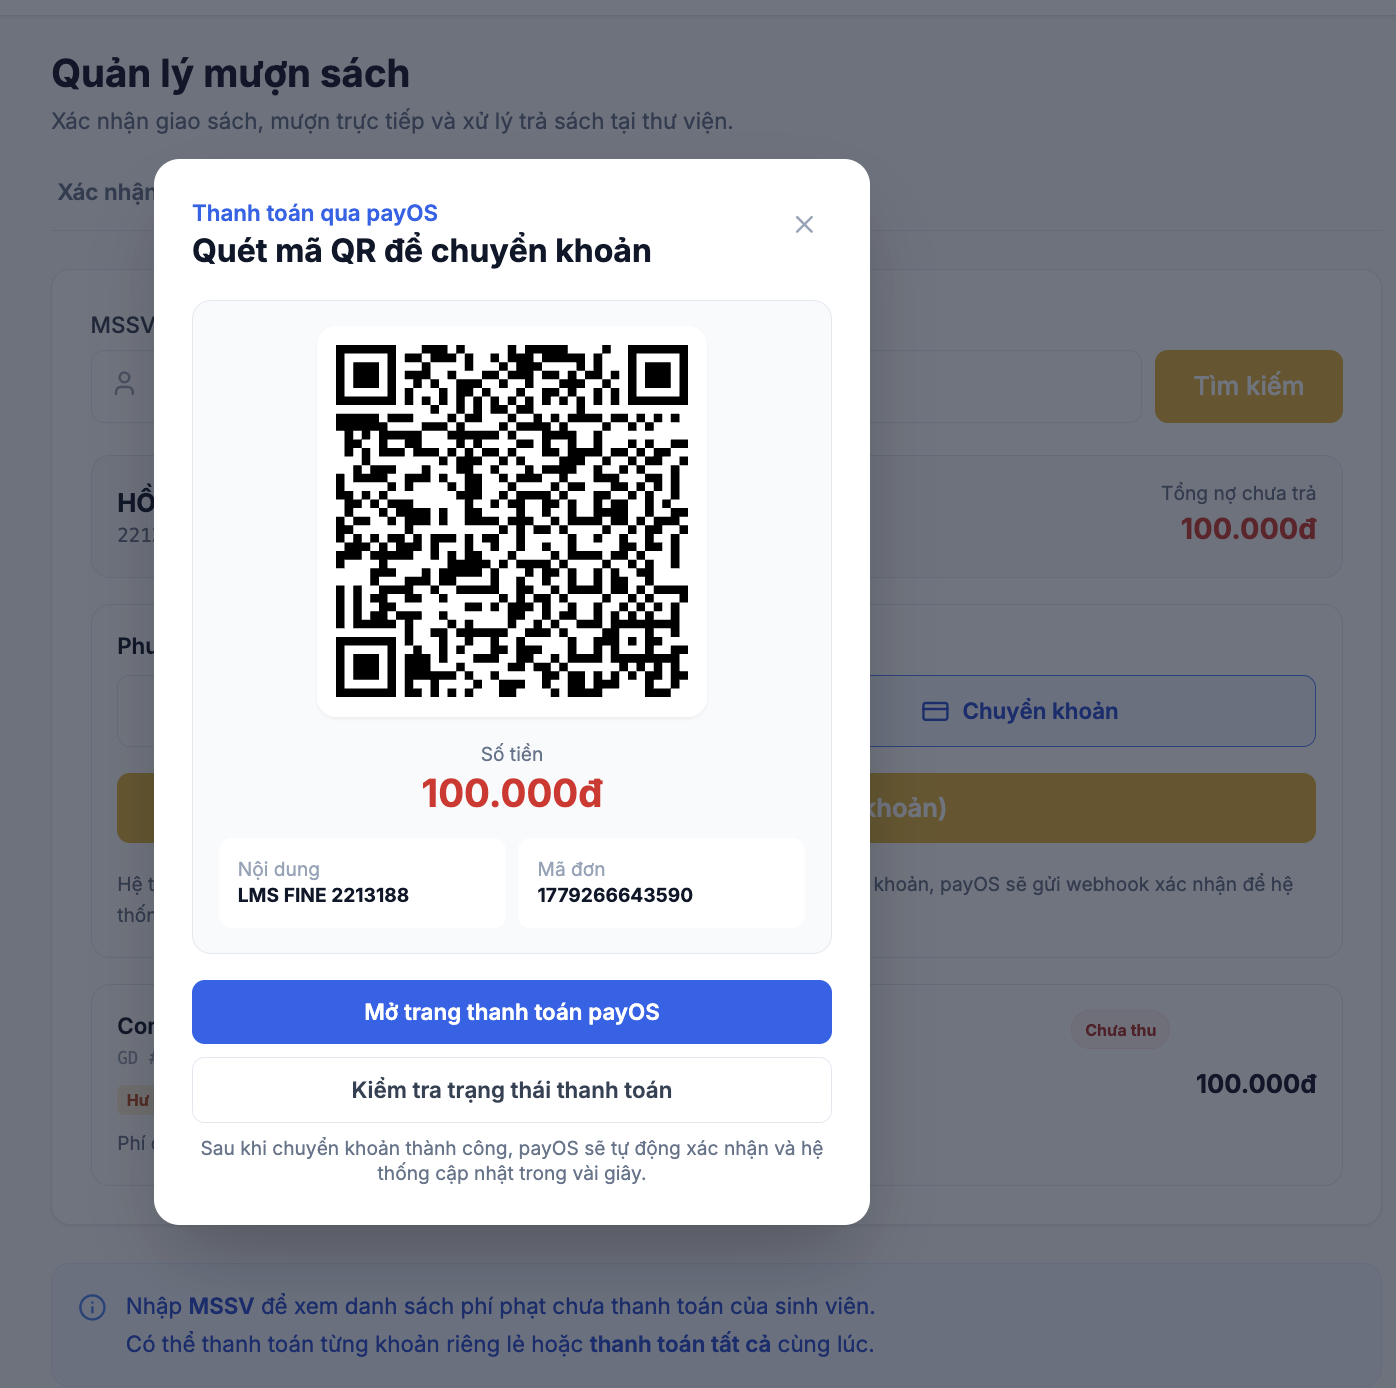
\includegraphics[width=\linewidth]{figures/ch06/payment/create_qr.png}
        \caption{Hiển thị mã QR PayOS}
    \end{subfigure}
    \caption{Quy trình tích hợp thanh toán tự động}
    \label{fig:fe_payment_integration}
\end{figure}

% ==========================================
% 2. PHÂN HỆ THỦ THƯ (LIBRARIAN FLOW)
% ==========================================
Đối với nghiệp vụ quản trị, hệ thống tập trung giải quyết bài toán giảm tải thao tác thủ công cho thủ thư bằng cách tự động hóa luồng số hóa tài liệu. Các tính năng nổi bật bao gồm tự động điền thông tin từ mã ISBN và giám sát tiến trình AI xử lý tài liệu vừa tải lên.

\begin{figure}[H]
    \centering
     \begin{subfigure}[b]{0.48\textwidth}
        \centering
        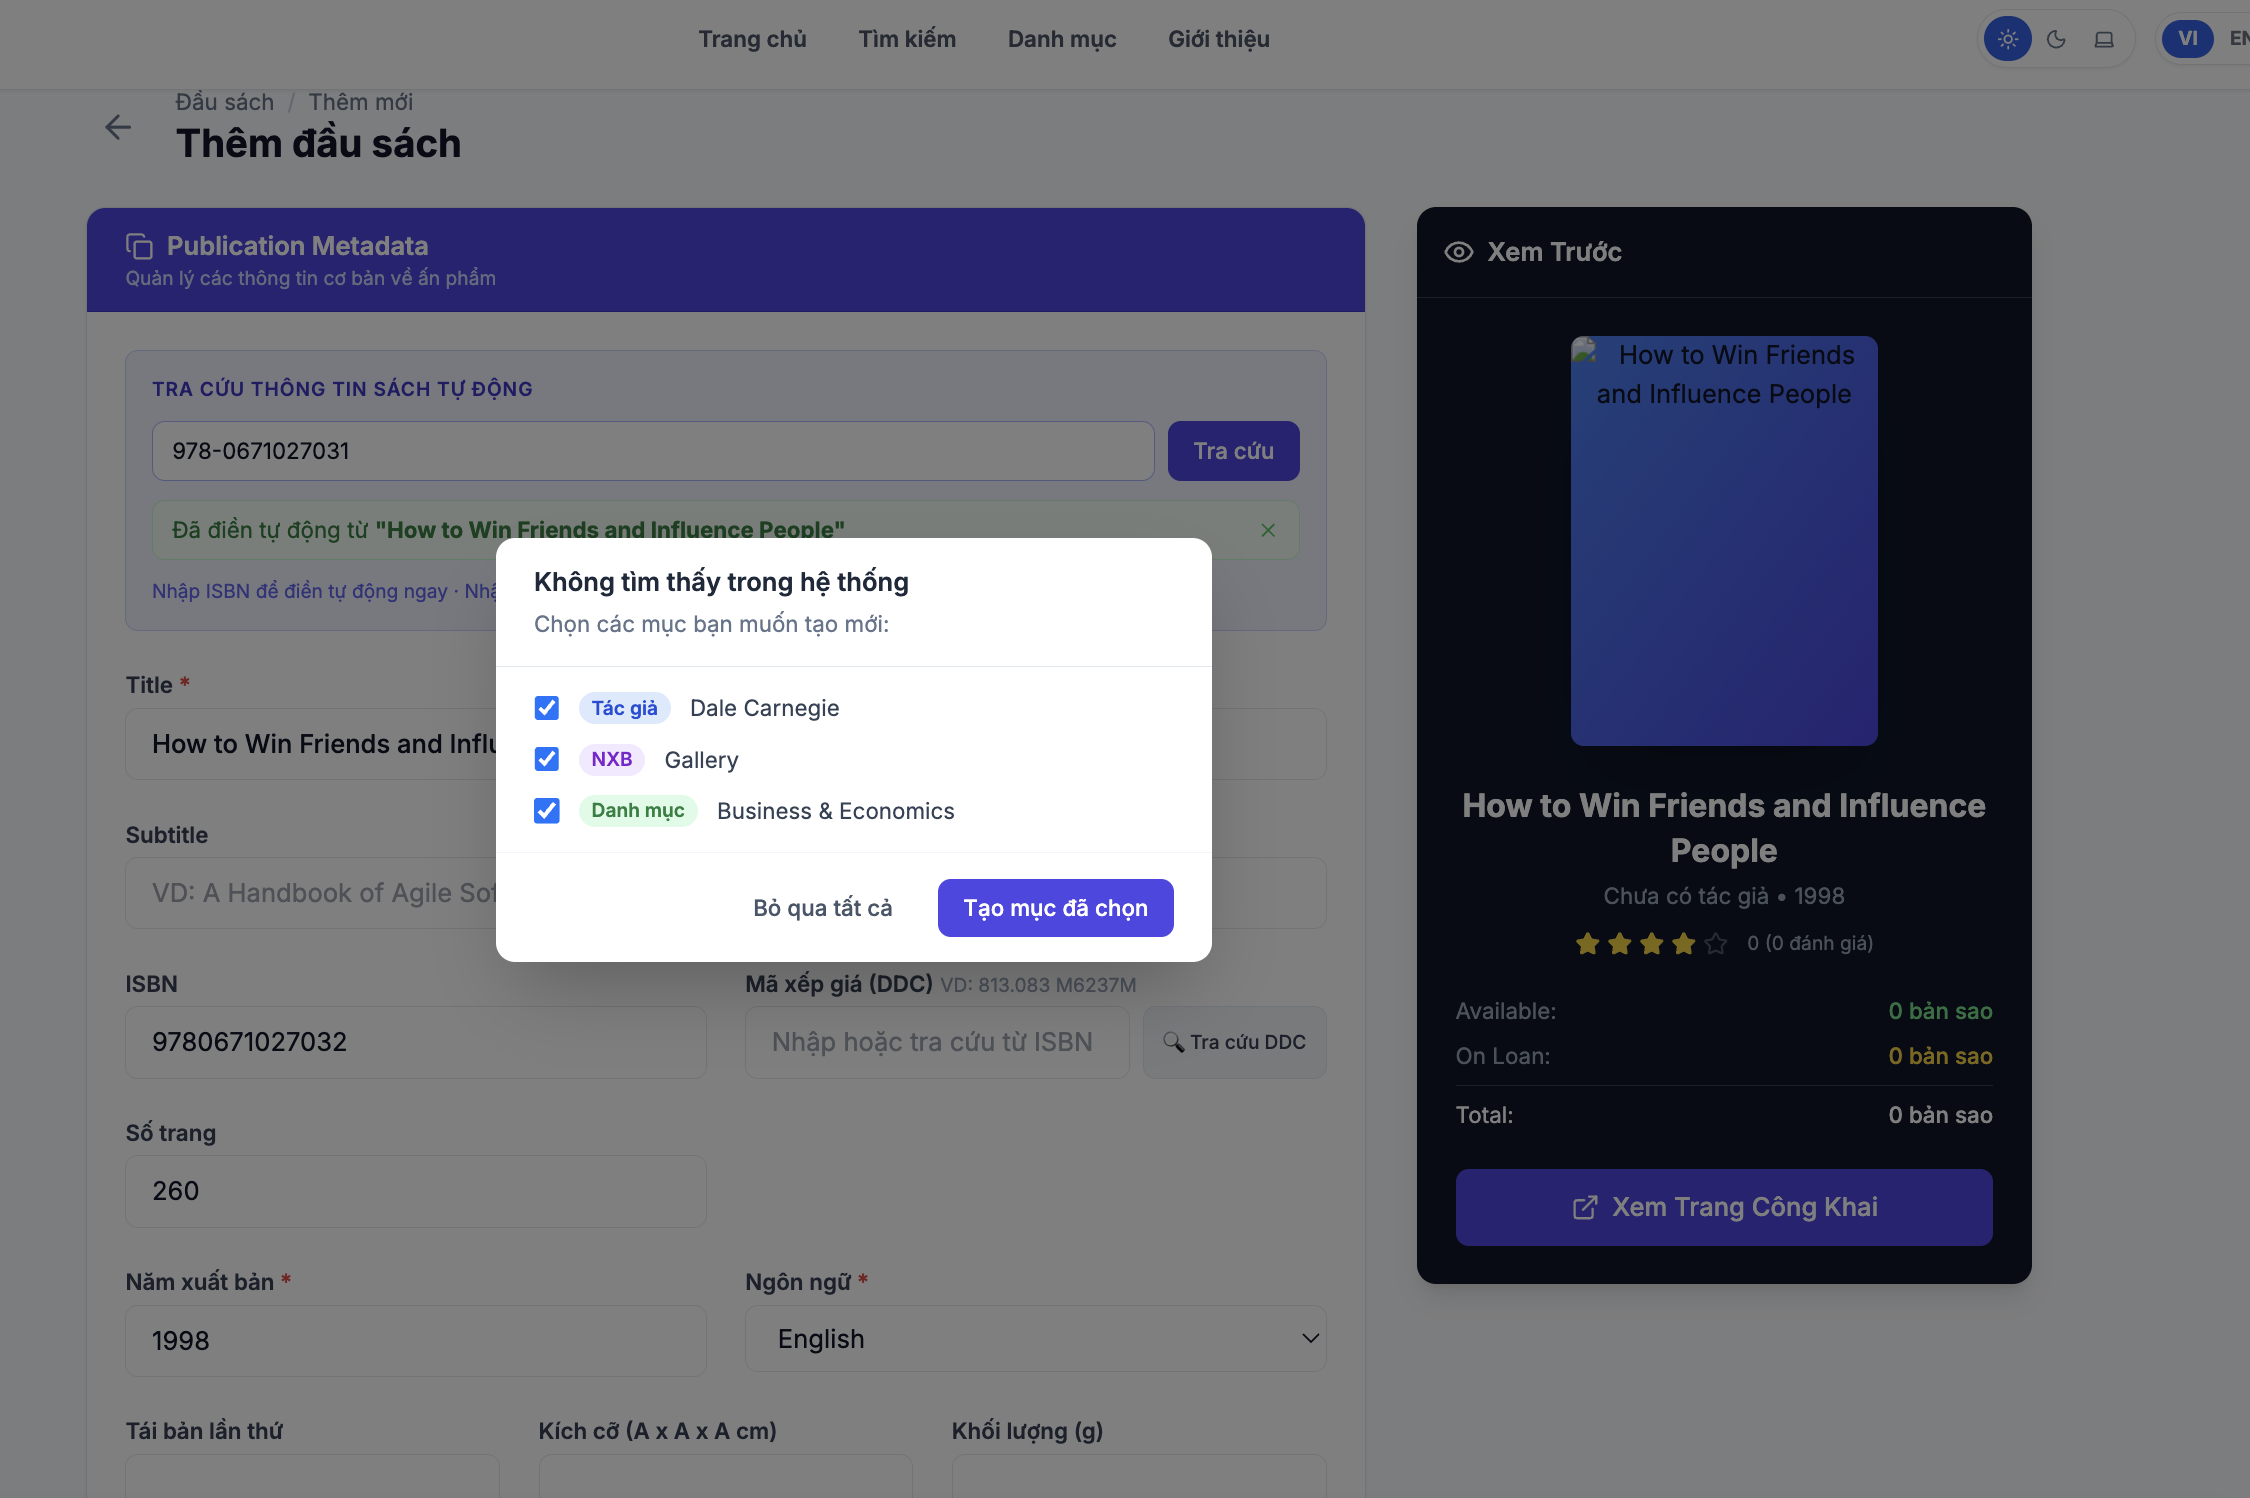
\includegraphics[width=\linewidth]{figures/ch06/frontend/isbn_auto_fill.png}
        \caption{Tự động trích xuất metadata từ ISBN}
    \end{subfigure}
    \hfill
        \begin{subfigure}[b]{0.48\textwidth}
        \centering
        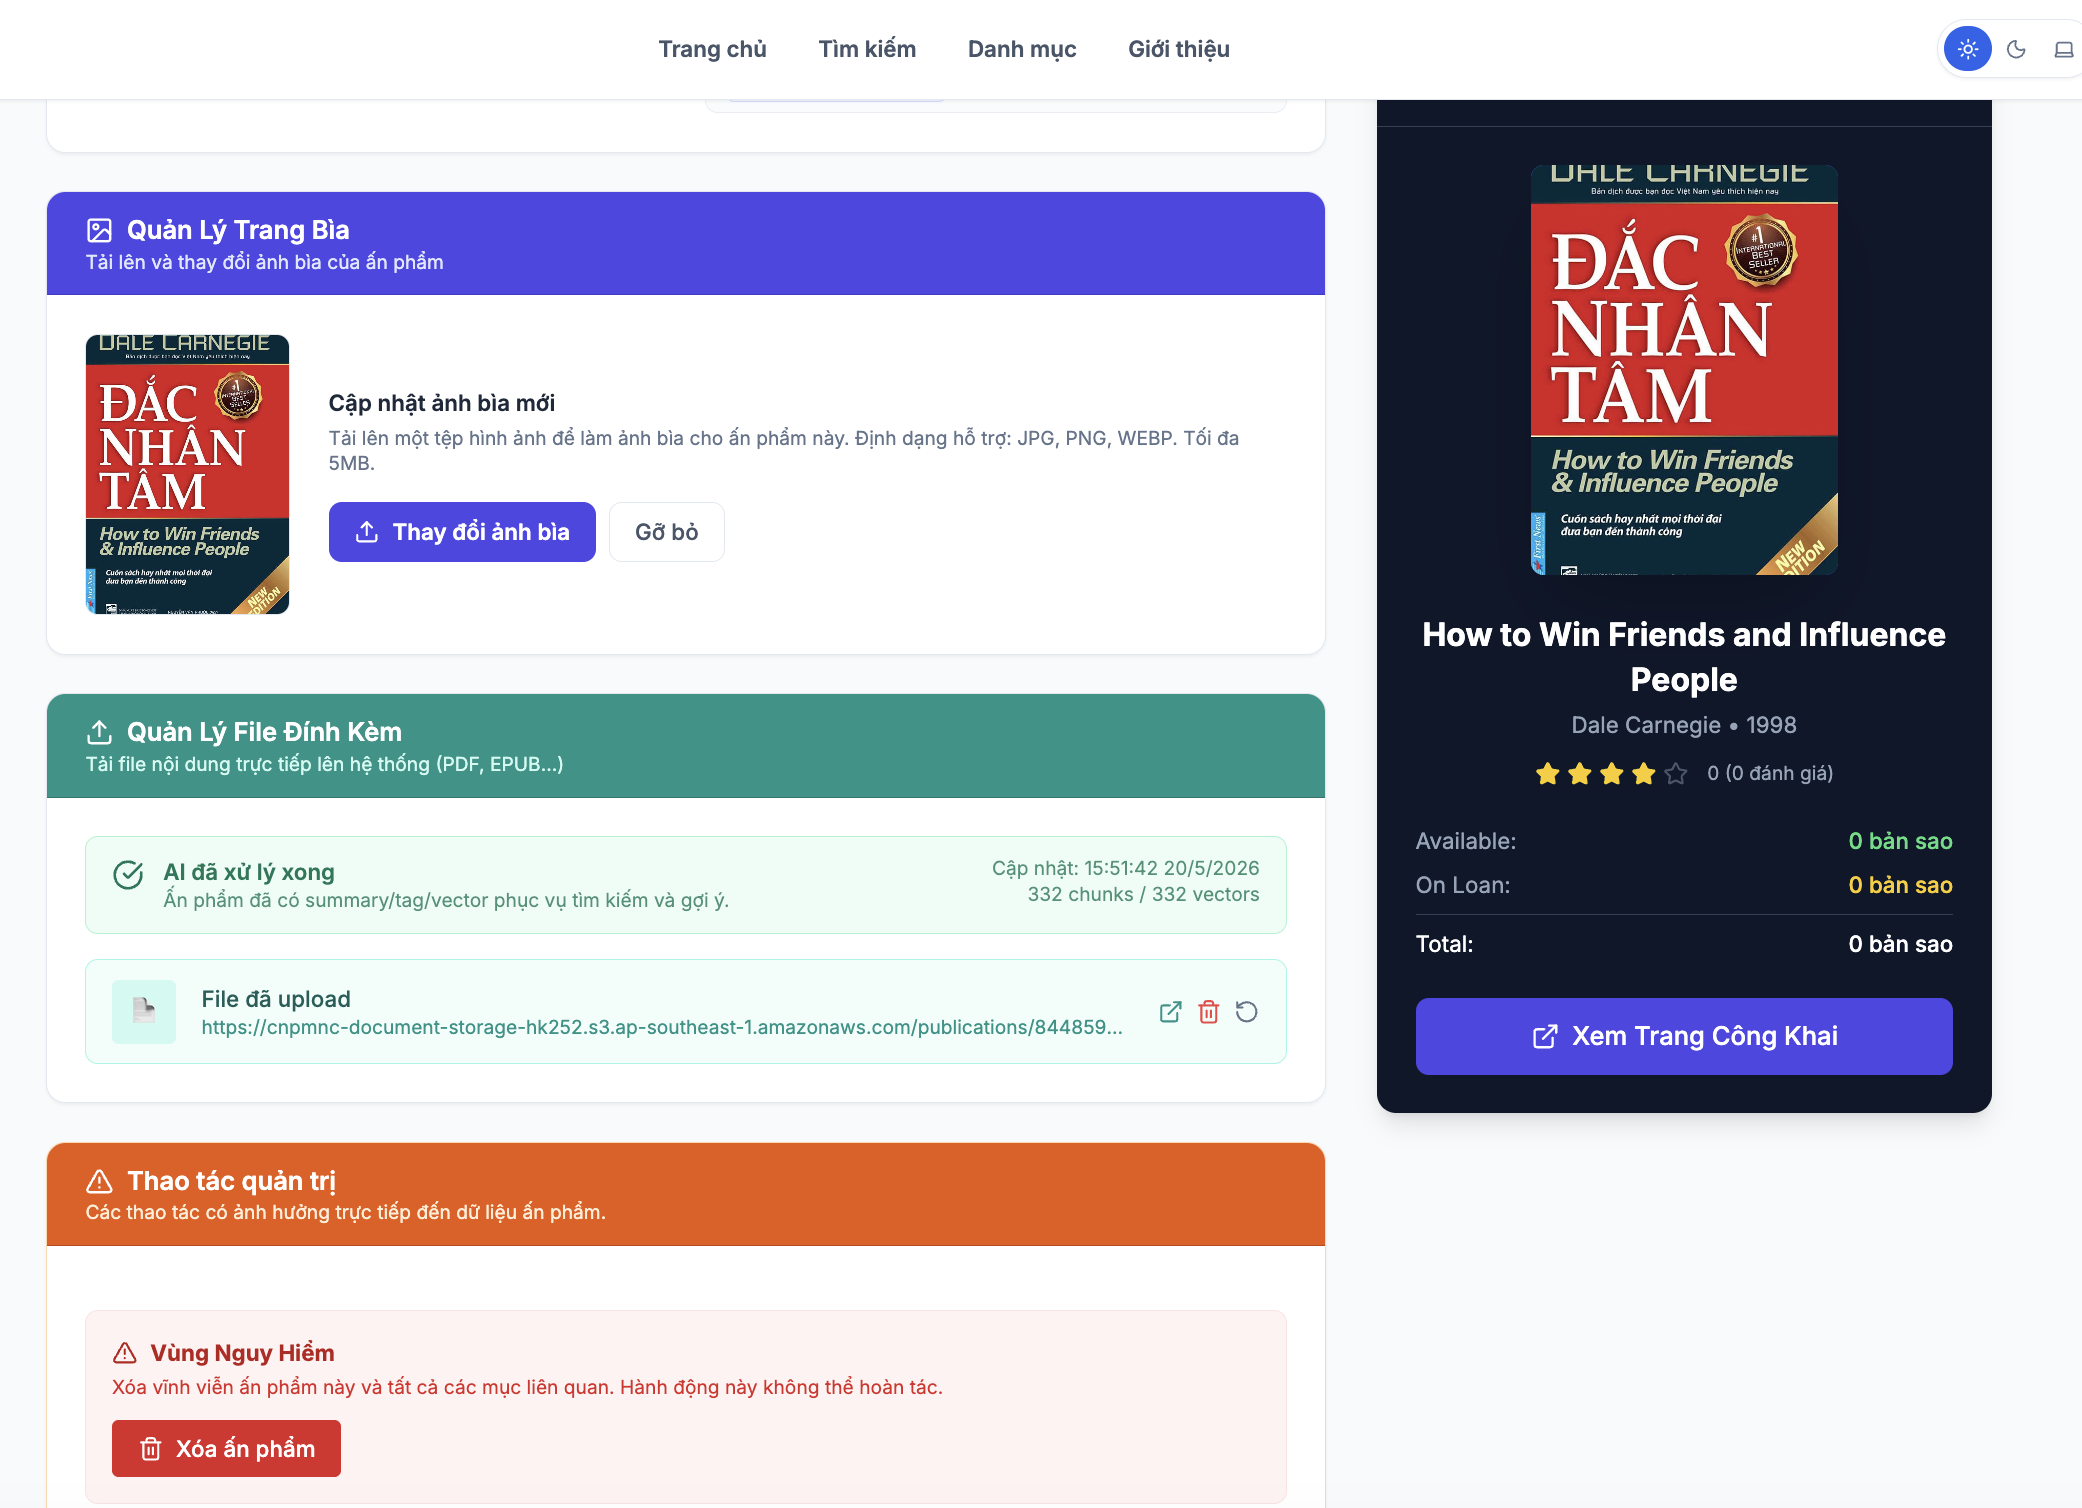
\includegraphics[width=\linewidth]{figures/ch06/frontend/upload_book.png}
        \caption{Tải lên tài liệu và giám sát tiến trình AI}
    \end{subfigure}
    \caption{Nghiệp vụ nhập liệu và số hóa tài liệu thông minh}
    \label{fig:fe_librarian_cataloging}
\end{figure}

Bên cạnh khâu nhập liệu, công tác giám sát và quản lý danh mục ấn phẩm cũng được trực quan hóa, kết hợp cùng hệ thống thông báo thời gian thực (real-time notification) để thủ thư nắm bắt và xử lý kịp thời các sự kiện phát sinh.

\begin{figure}[H]
    \centering
    \begin{subfigure}[b]{0.48\textwidth}
        \centering
        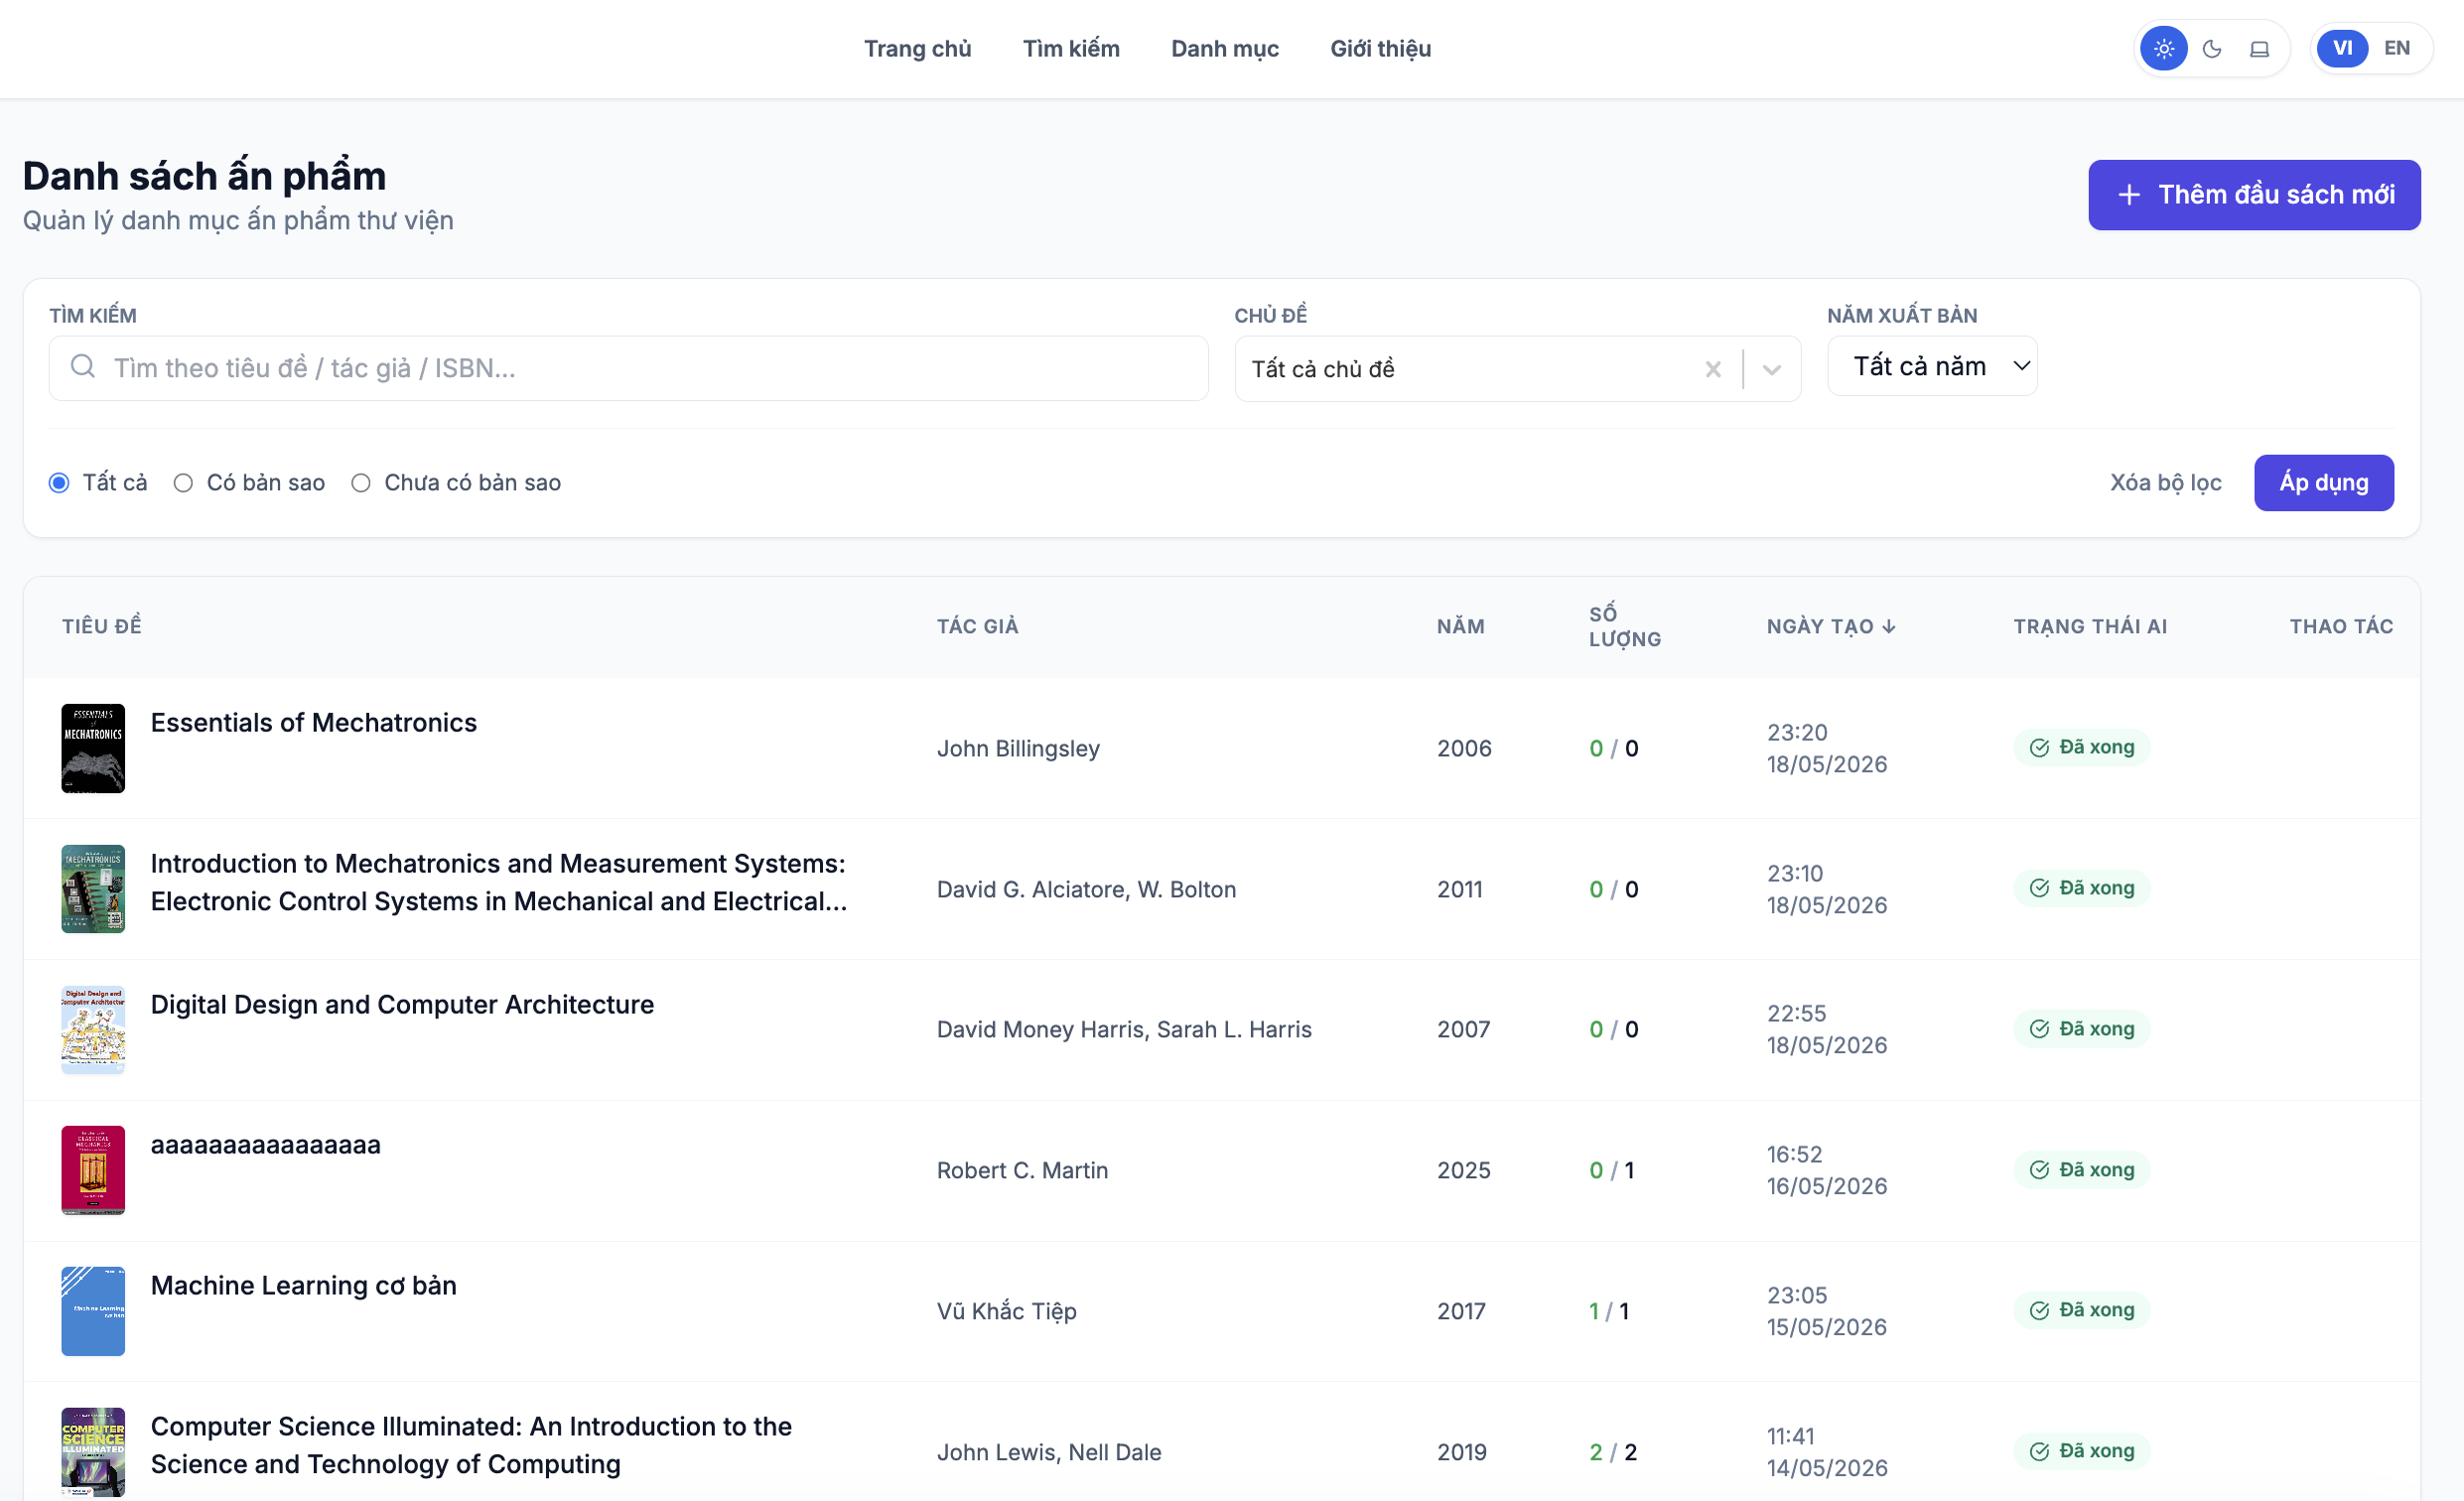
\includegraphics[width=\linewidth]{figures/ch06/frontend/publication_management.png}
        \caption{Quản lý danh mục ấn phẩm}
    \end{subfigure}
    \hfill
        \begin{subfigure}[b]{0.48\textwidth}
        \centering
        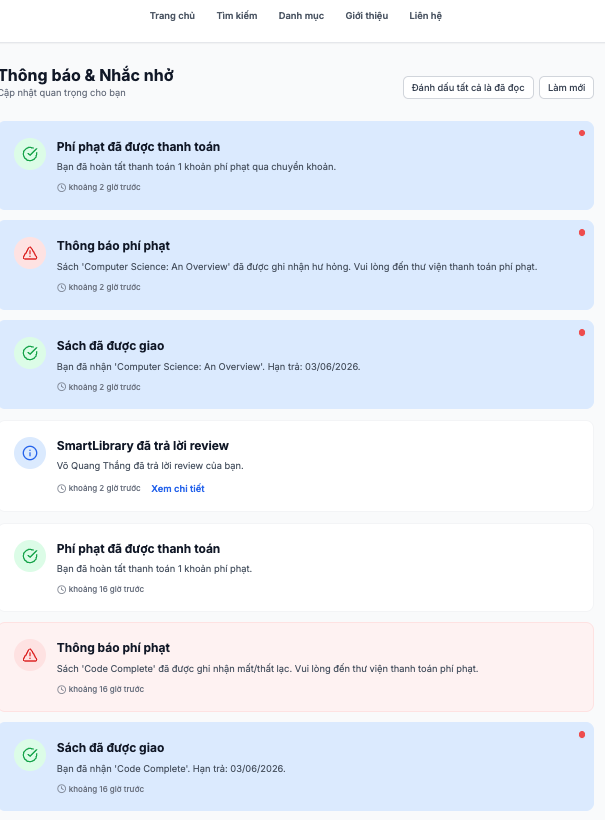
\includegraphics[width=\linewidth]{figures/ch06/frontend/realtime_notification.png}
        \caption{Hệ thống thông báo thời gian thực}
    \end{subfigure}
    \caption{Nghiệp vụ quản lý vận hành và giám sát hệ thống của thủ thư}
    \label{fig:fe_librarian_management}
\end{figure}

% ==========================================
% 3. GIAO TIẾP VÀ CẤU HÌNH HỆ THỐNG
% ==========================================
Cuối cùng, để đảm bảo tính kết nối và đáp ứng đa dạng nhu cầu sử dụng, hệ thống cung cấp luồng giao tiếp hỗ trợ trực tuyến giữa các nhóm người dùng, đi kèm các tùy chọn cá nhân hóa sâu về giao diện (Light/Dark mode) và ngôn ngữ (Việt - Anh).

\begin{figure}[H]
    \centering
    \begin{subfigure}[b]{0.48\textwidth}
        \centering
        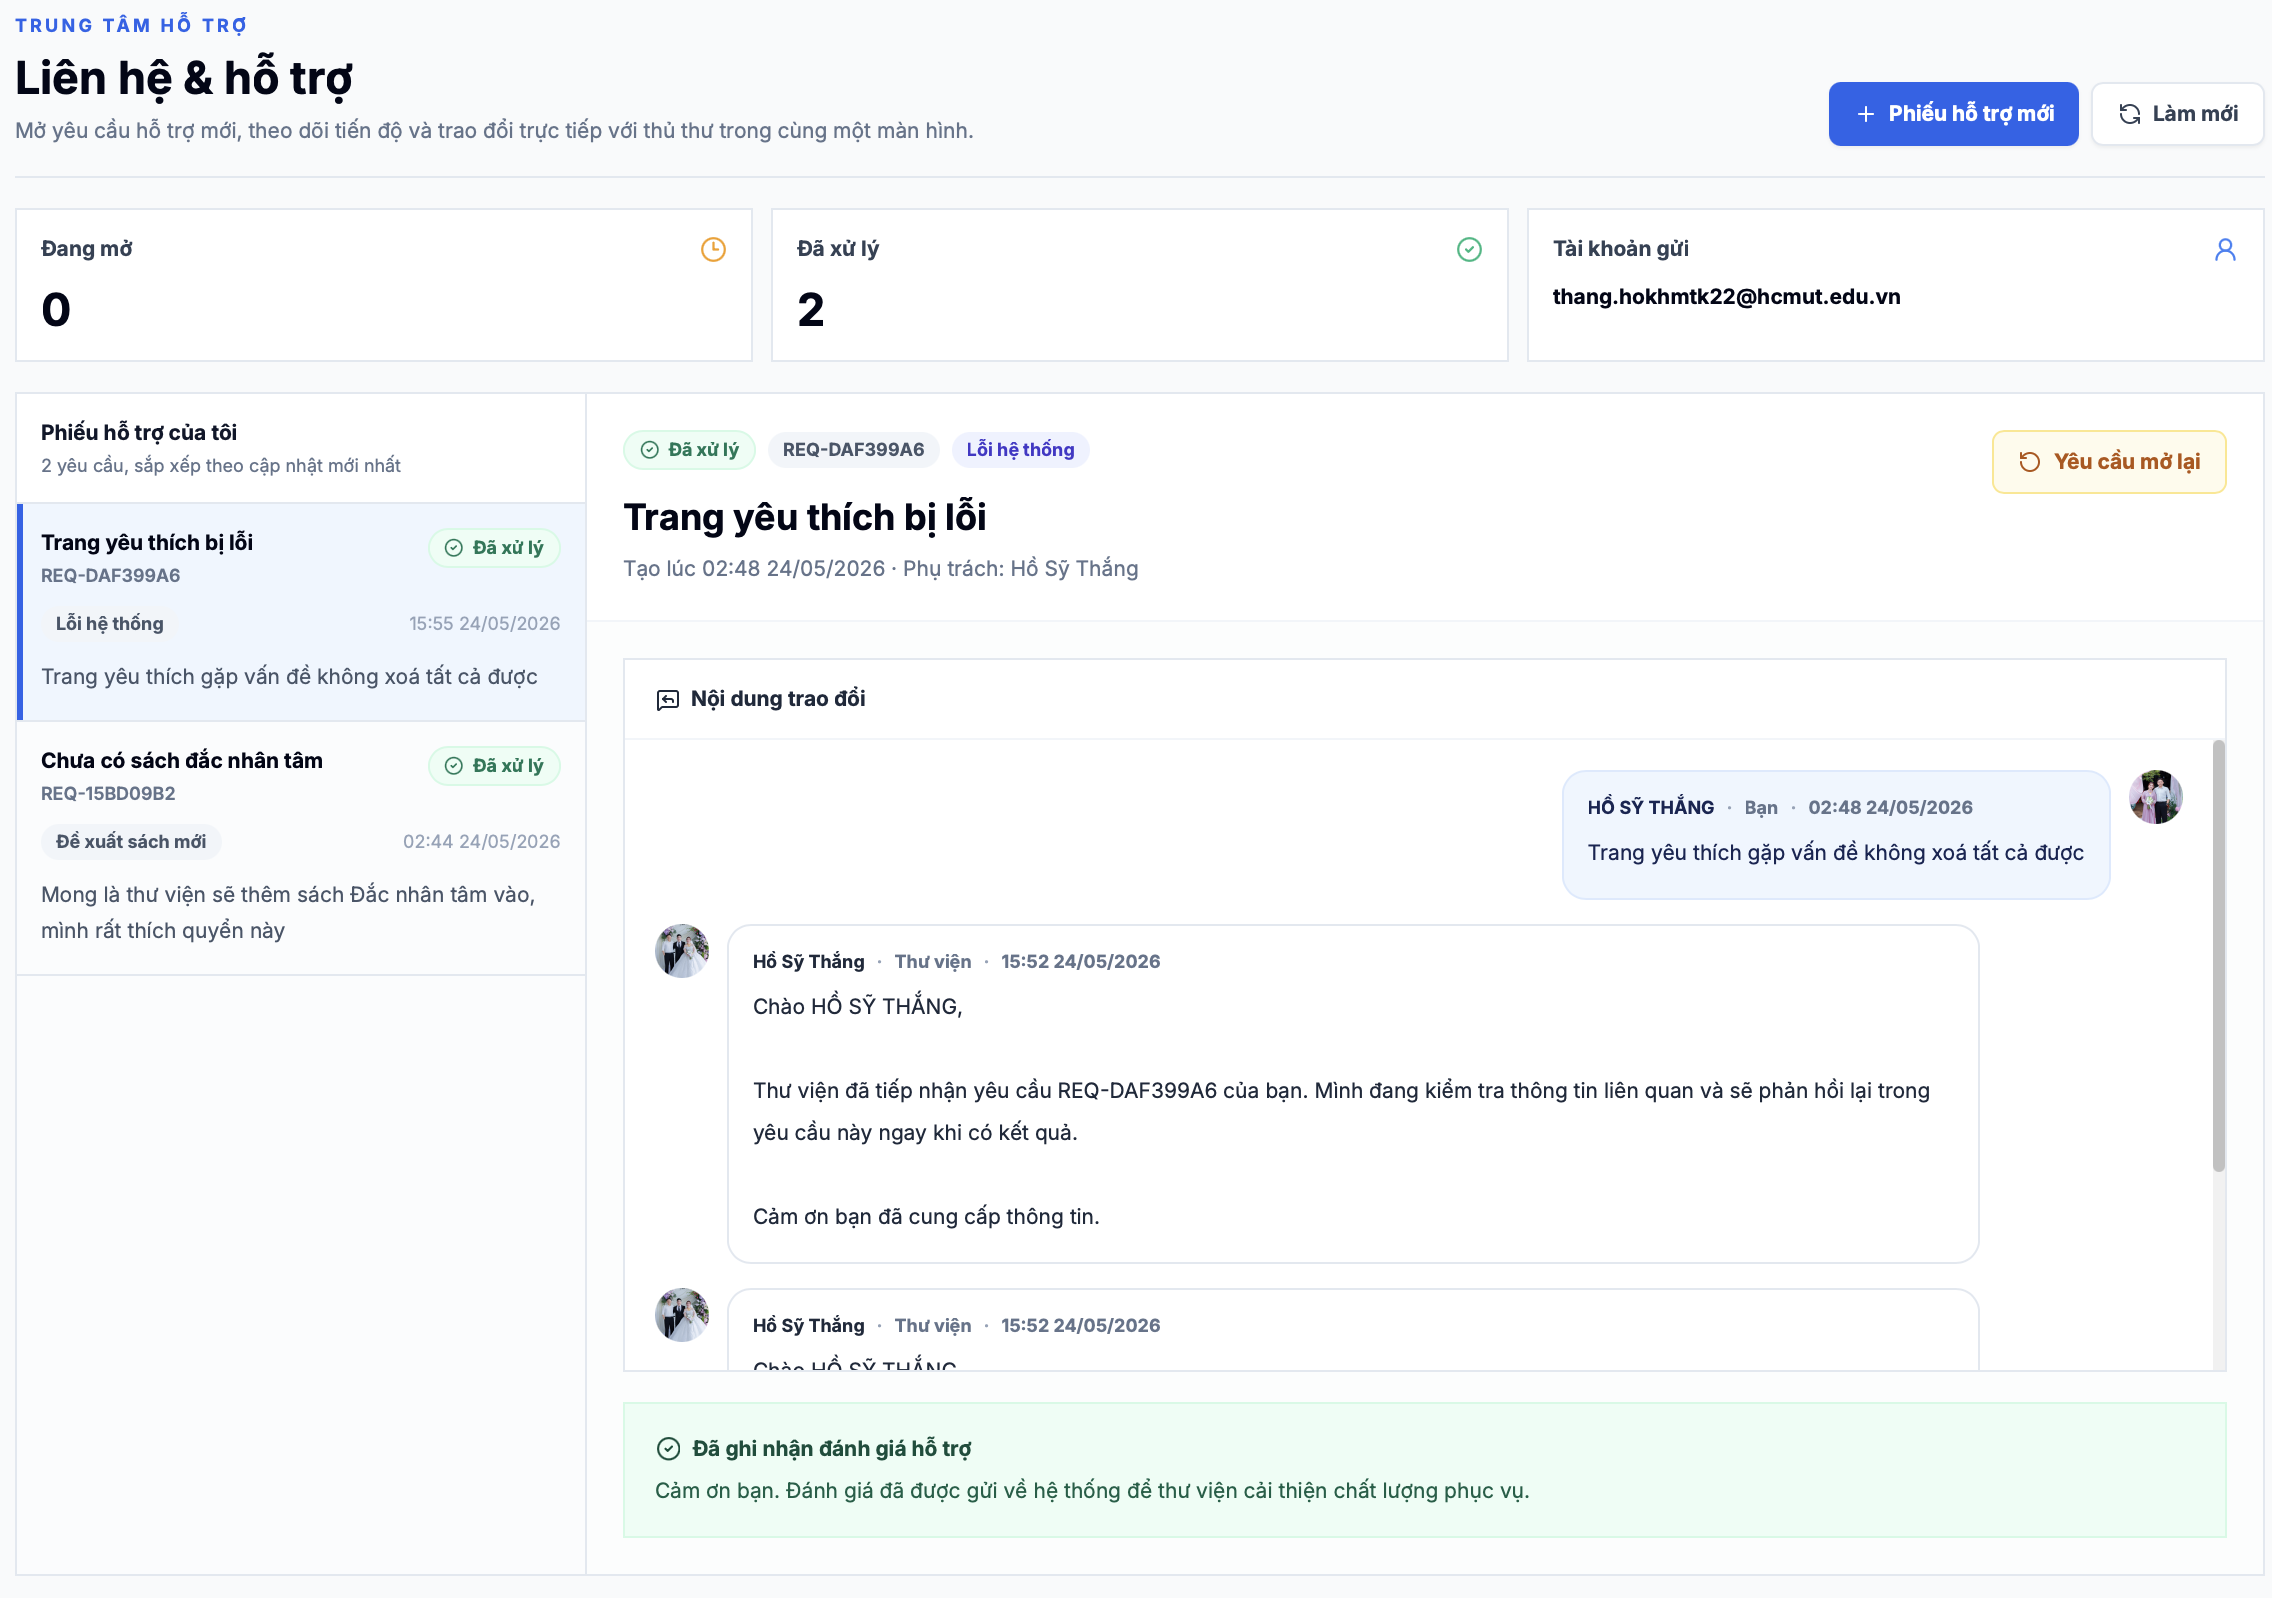
\includegraphics[width=\linewidth]{figures/ch06/frontend/contact_and_support_user.png}
        \caption{Gửi yêu cầu hỗ trợ (Bạn đọc)}
    \end{subfigure}
    \hfill
    \begin{subfigure}[b]{0.48\textwidth}
        \centering
        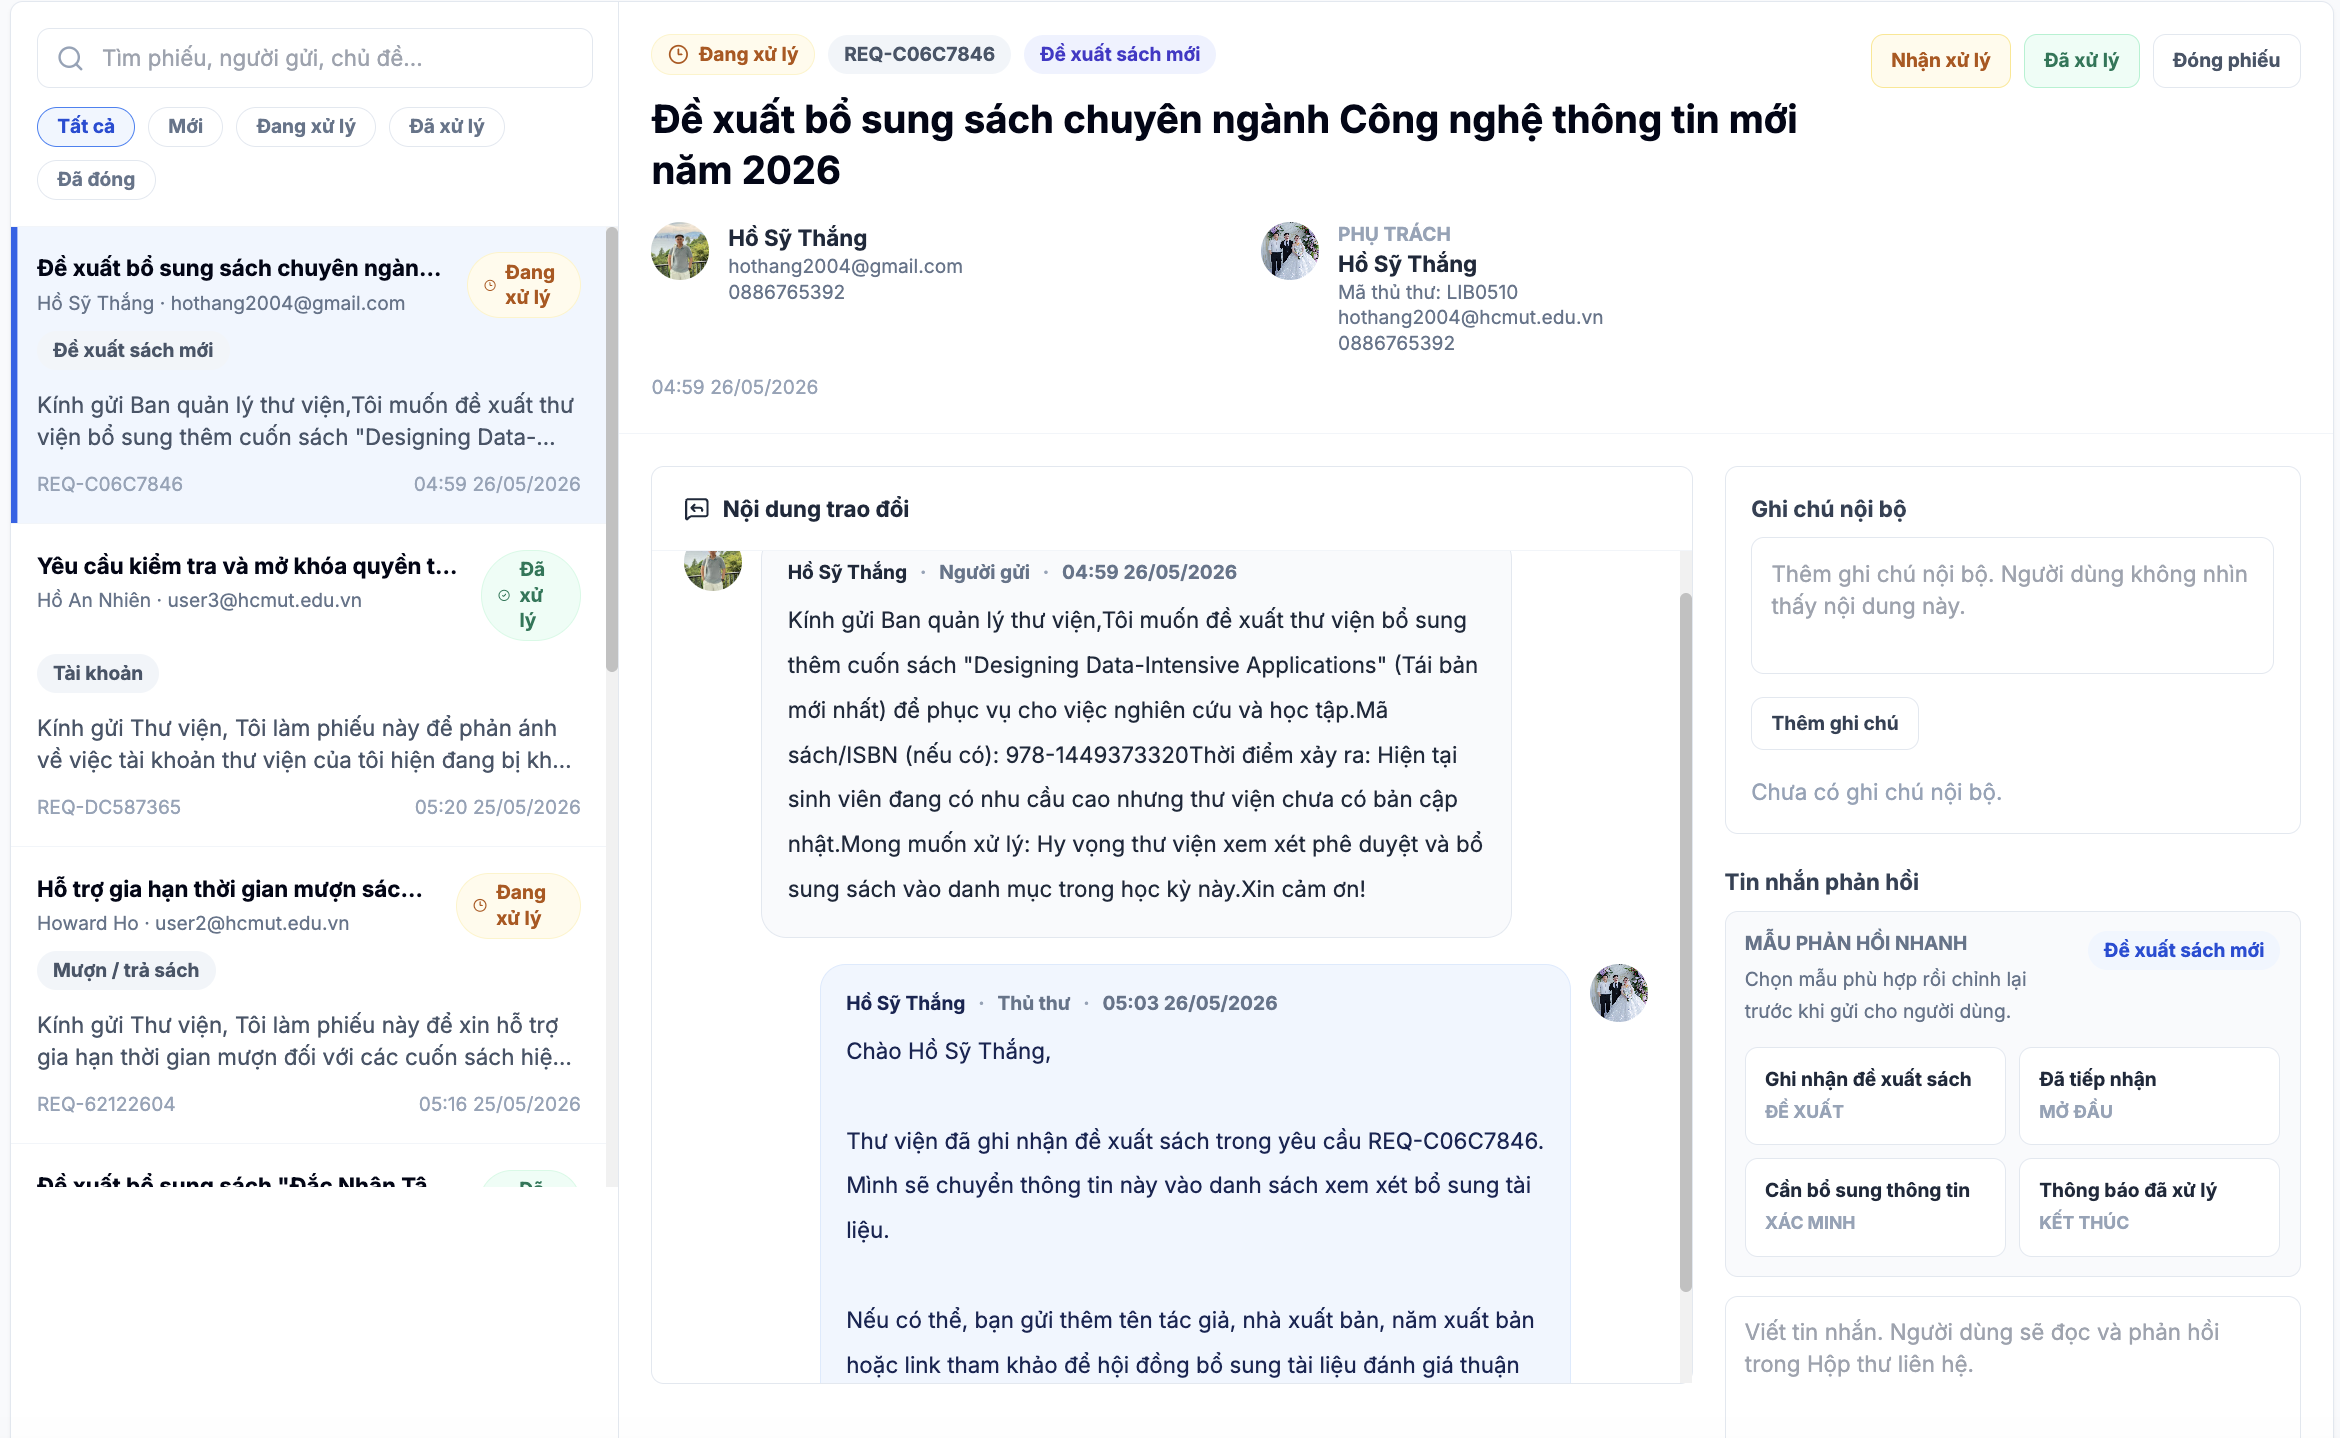
\includegraphics[width=\linewidth]{figures/ch06/frontend/contact_and_support_librarian.png}
        \caption{Tiếp nhận và phản hồi (Thủ thư)}
    \end{subfigure}
    \caption{Luồng giao tiếp và hỗ trợ trực tuyến giữa các nhóm người dùng}
    \label{fig:fe_cross_support}
\end{figure}

\begin{figure}[H]
    \centering
    \begin{subfigure}[b]{0.48\textwidth}
        \centering
        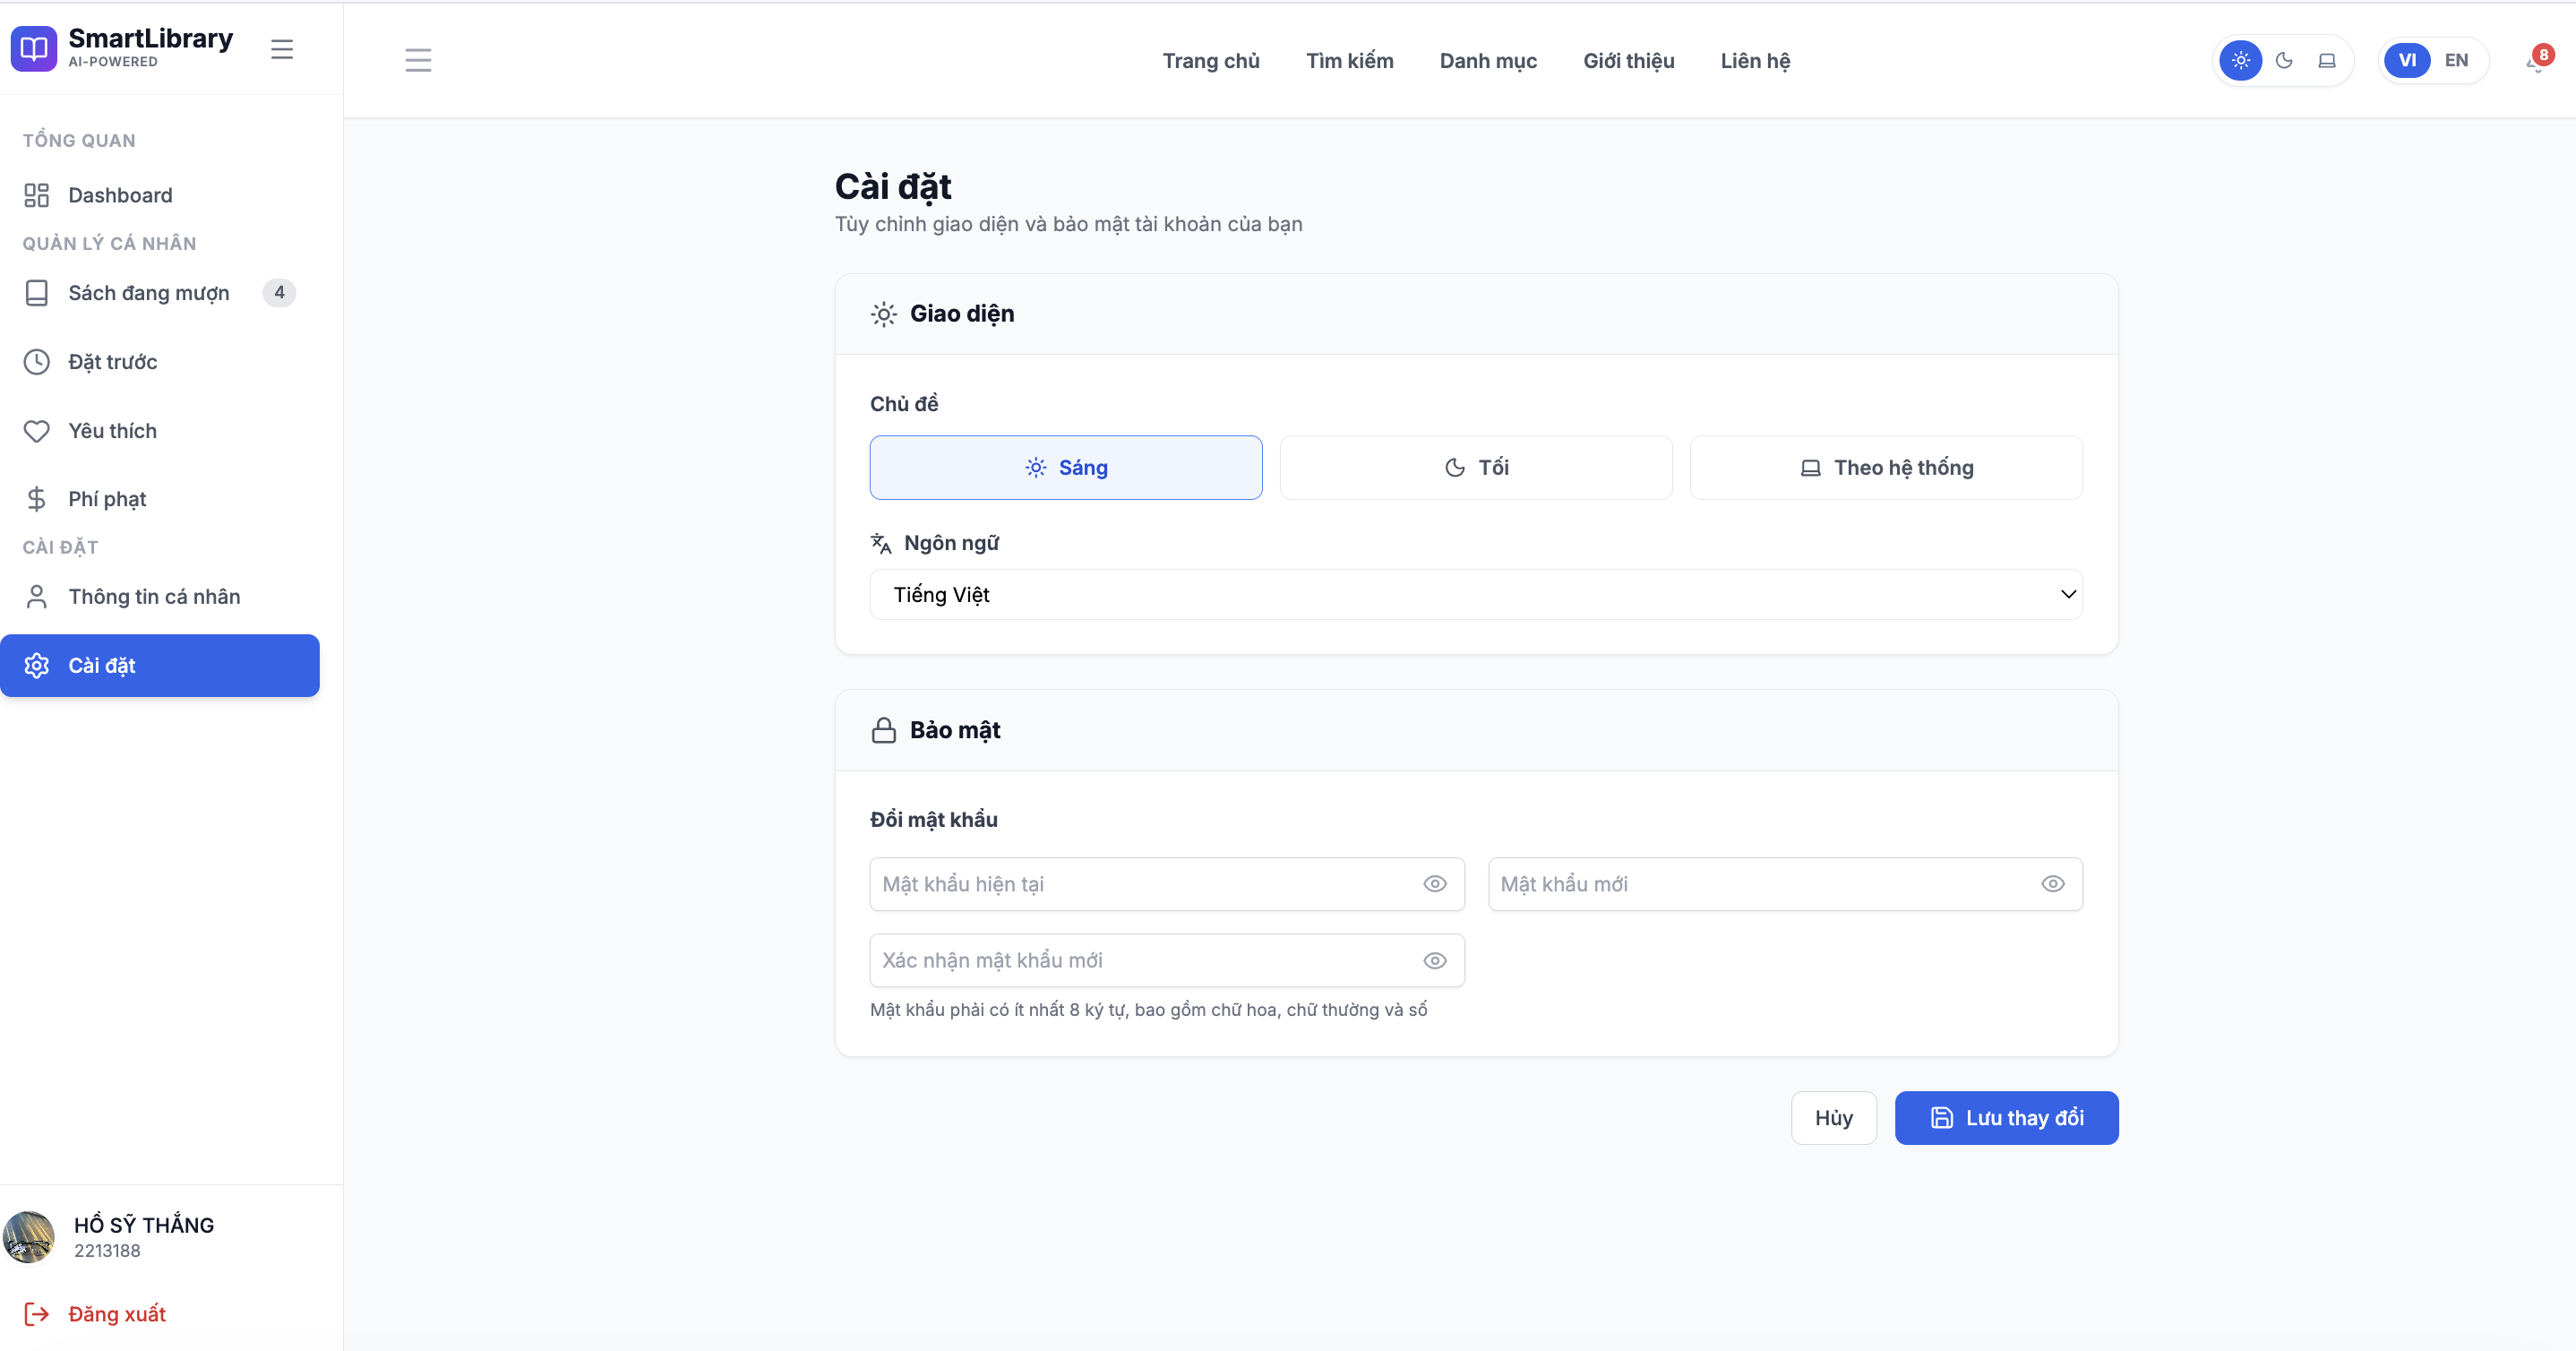
\includegraphics[width=\linewidth]{figures/ch06/frontend/light_theme_and_vietnamese.png}
        \caption{Giao diện sáng (Light) - Tiếng Việt}
    \end{subfigure}
    \hfill
    \begin{subfigure}[b]{0.48\textwidth}
        \centering
        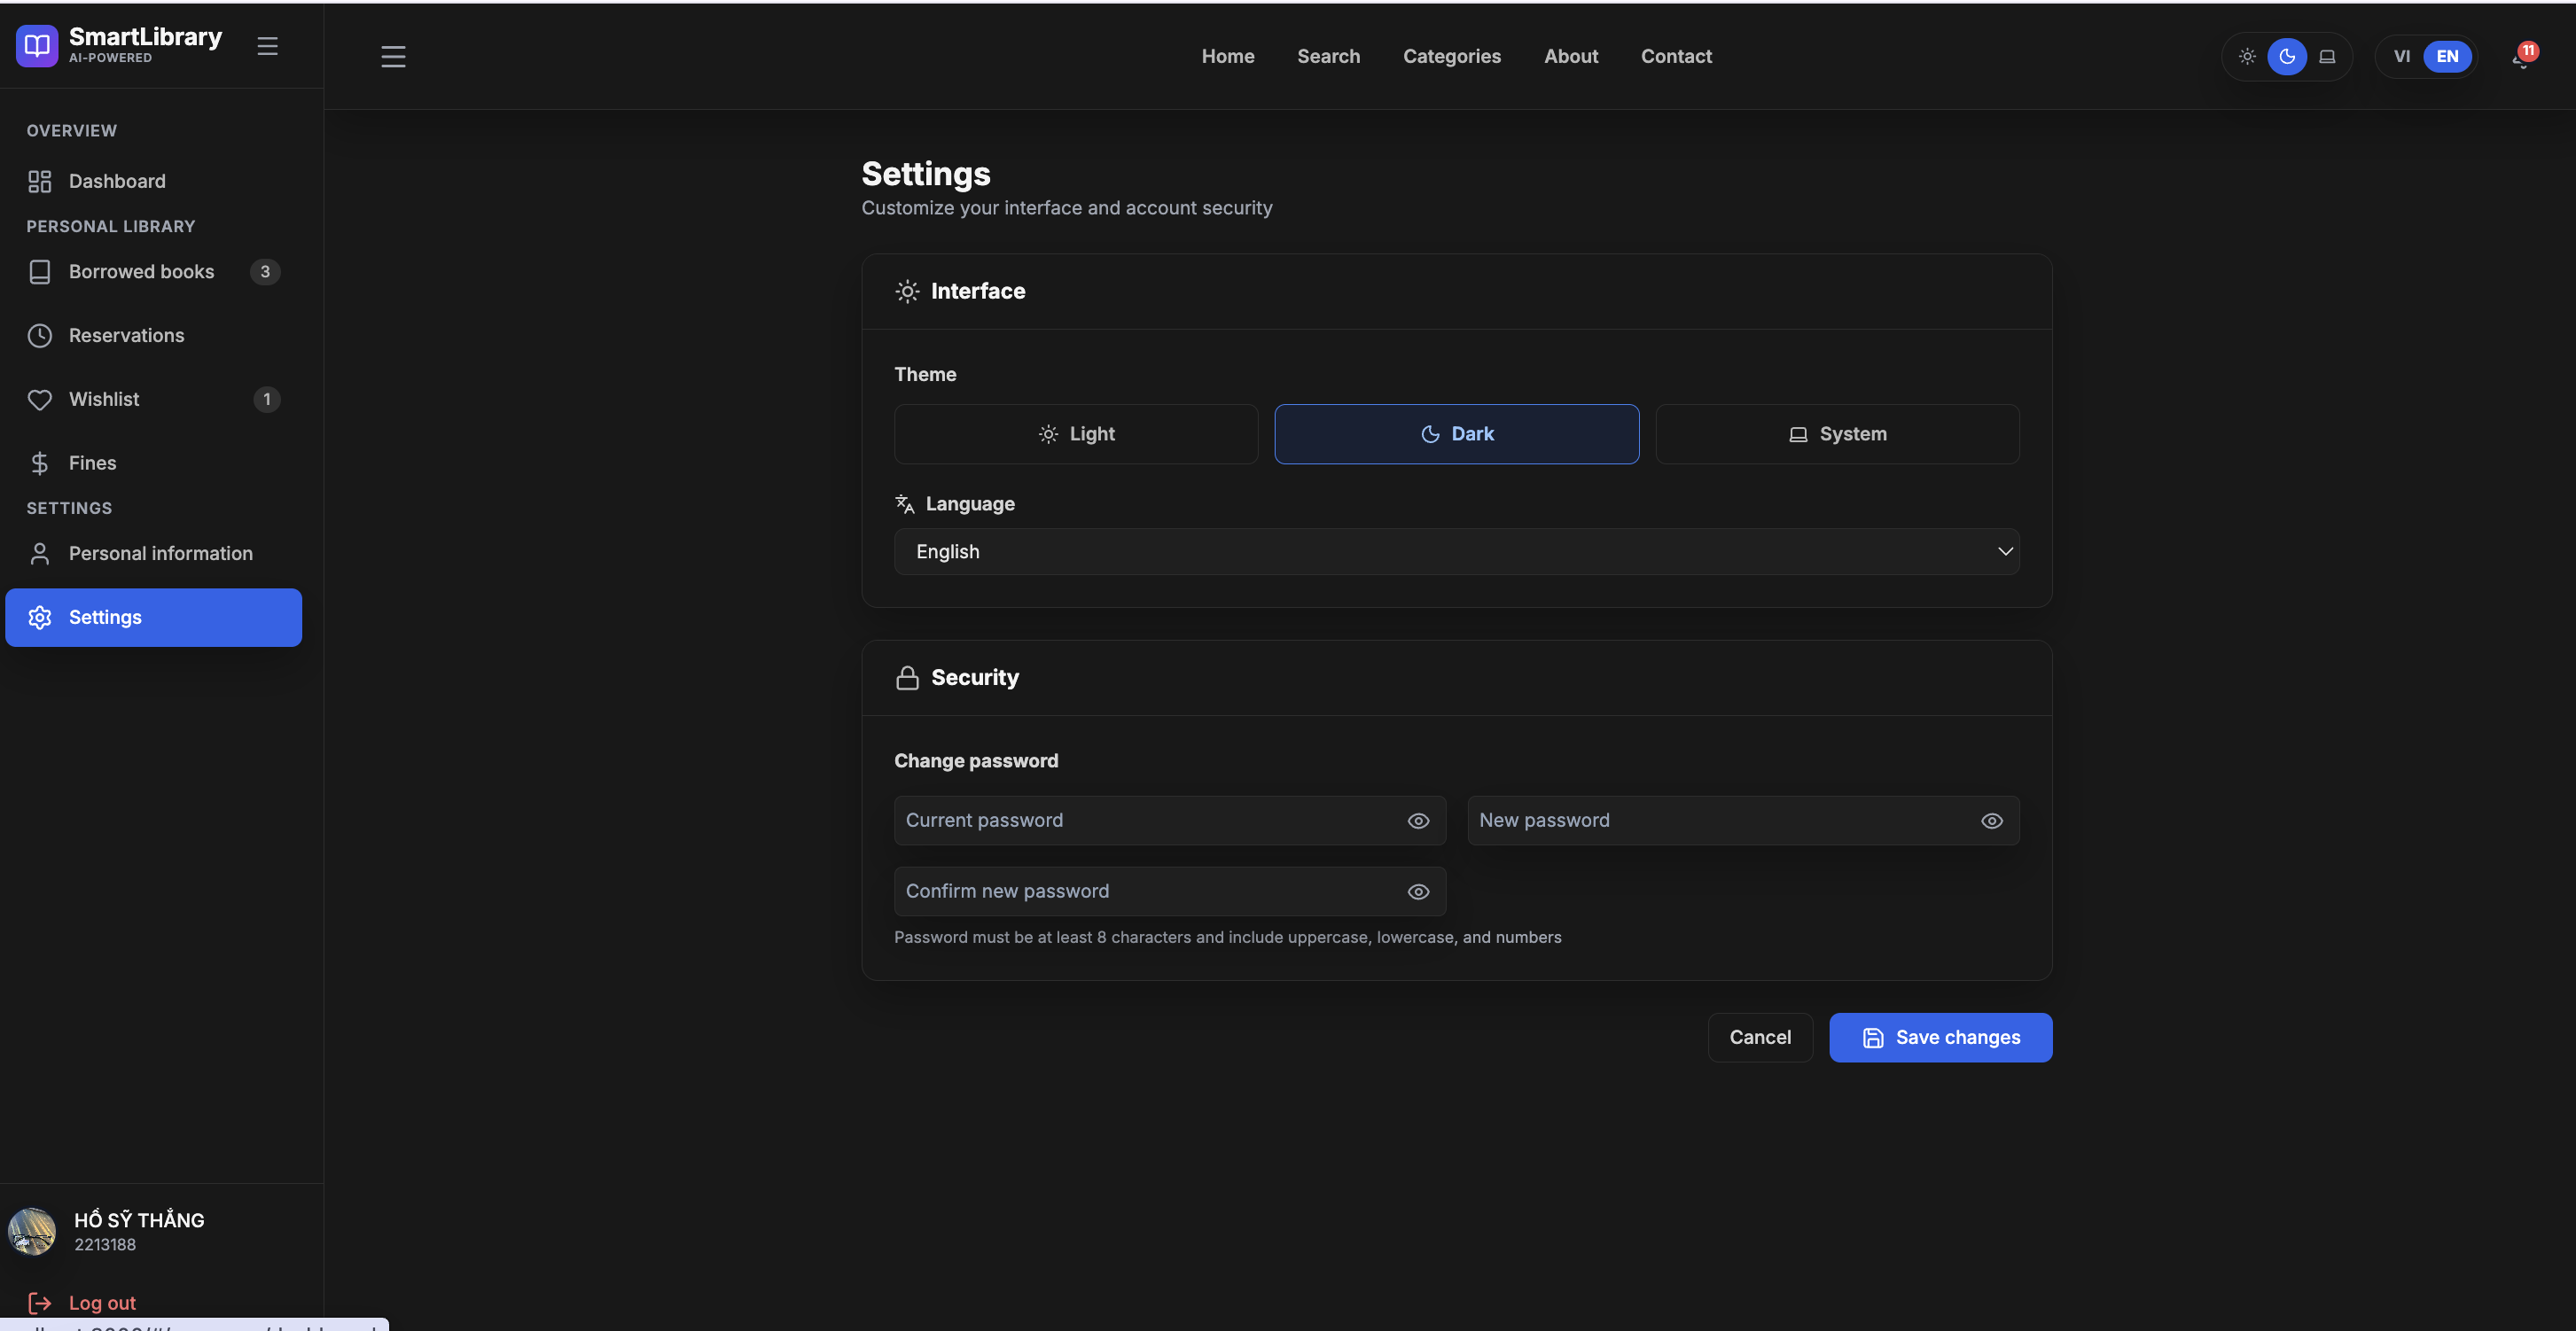
\includegraphics[width=\linewidth]{figures/ch06/frontend/dark_theme_and_english.png}
        \caption{Giao diện tối (Dark) - Tiếng Anh}
    \end{subfigure}
    \caption{Tính năng cá nhân hóa giao diện và đa ngôn ngữ (i18n)}
    \label{fig:fe_system_personalization}
\end{figure}

% --- ĐOẠN CHUYỂN Ý 1: TỪ GIAO DIỆN SANG KỸ THUẬT ---
Đằng sau giao diện trực quan và các trải nghiệm cá nhân hóa linh hoạt, phân hệ Frontend được xây dựng dựa trên một kiến trúc kỹ thuật vững chắc nhằm đảm bảo tính mở rộng và hiệu năng cao. Bảng \ref{tab:fe_technical_summary} tổng hợp các giải pháp kỹ thuật trọng tâm đã được áp dụng để giải quyết các bài toán cốt lõi: từ quản lý trạng thái tập trung, tối ưu giao tiếp API, đến xử lý luồng sự kiện thời gian thực (real-time) và tích hợp an toàn các dịch vụ bên thứ ba.

\begin{table}[H]
\centering
\small
\begin{tabularx}{\textwidth}{|p{3.4cm}|X|}
\hline
\textbf{Hạng mục Frontend} & \textbf{Nội dung đã hiện thực} \\
\hline
Routing và phân quyền &
\texttt{HashRouter}, lazy loading theo page, \texttt{ProtectedRoute}, redirect
theo role \texttt{student}, \texttt{librarian}, \texttt{admin}. \\
\hline
State dùng chung &
\texttt{AuthContext}, \texttt{LanguageContext}, \texttt{ThemeContext},
\texttt{NotificationContext}, \texttt{UploadContext}, \texttt{AppDialogContext}. \\
\hline
Giao tiếp API &
Axios instance, gắn JWT và \texttt{Accept-Language}, unwrap response, xử lý lỗi
nghiệp vụ, refresh token bằng queue để tránh gọi refresh nhiều lần. \\
\hline
Realtime và notification &
STOMP/SockJS, unread count, toast realtime, đánh dấu đã đọc và đồng bộ danh sách
thông báo. \\
\hline
Upload và tài liệu &
Upload bìa/PDF bằng presigned URL, hiển thị progress, cảnh báo khi đóng tab lúc
upload đang chạy, gửi yêu cầu AI xử lý tài liệu. \\
\hline
Thanh toán &
Khởi tạo thanh toán PayOS, hiển thị QR, polling trạng thái, cập nhật UI cho thủ
thư và bạn đọc sau khi thanh toán. \\
\hline
Cá nhân hóa &
Light/dark/system theme, song ngữ Việt--Anh, lưu cấu hình vào
\texttt{localStorage}, cập nhật \texttt{document.lang}. \\
\hline
\end{tabularx}
\caption{Các hạng mục kỹ thuật Frontend}
\label{tab:fe_technical_summary}
\end{table}

% --- ĐOẠN CHUYỂN Ý 2: TỪ KỸ THUẬT SANG GIÁ TRỊ THỰC TIỄN ---
Tất cả các quyết định về mặt kiến trúc và kỹ thuật nêu trên đều hướng tới một mục tiêu duy nhất: chuyển hóa công nghệ thành giá trị sử dụng. Bảng \ref{tab:fe_value_highlights} đúc kết lại những điểm sáng nổi bật của phân hệ, minh chứng cho việc ứng dụng công nghệ không chỉ dừng lại ở mặt hiển thị mà đã thực sự giải quyết triệt để các bài toán vận hành, chuyển đổi toàn diện trải nghiệm của bạn đọc và thủ thư.

\begin{table}[H]
\centering
\small
\begin{tabularx}{\textwidth}{|p{3.4cm}|X|p{3.4cm}|}
\hline
\textbf{Giá trị hiện thực} & \textbf{Cách hệ thống đã làm} & \textbf{Tác động với người dùng} \\
\hline
Tìm kiếm đa hướng &
Kết hợp keyword search, bộ lọc catalog, tag/category alias và semantic search. &
Bạn đọc không cần nhớ chính xác tên sách vẫn có thể tìm tài liệu phù hợp. \\
\hline
Vận hành tại quầy &
Màn hình thủ thư hỗ trợ mượn trực tiếp, xác nhận nhận sách, trả sách, ghi chú và xử lý phí. &
Nghiệp vụ mượn--trả không còn chỉ nằm ở phần demo giao diện. \\
\hline
Tài liệu số &
Upload bìa/PDF, progress upload, presigned URL và kích hoạt AI xử lý nền. &
Thủ thư có thể đưa tài liệu mới vào hệ thống và theo dõi kết quả xử lý. \\
\hline
Phản hồi tức thời &
Toast, notification realtime, unread count và đồng bộ trạng thái thanh toán/đặt trước. &
Người dùng biết ngay khi có thay đổi quan trọng thay vì phải tải lại trang. \\
\hline
\end{tabularx}
\caption{Các điểm giá trị nổi bật ở Frontend}
\label{tab:fe_value_highlights}
\end{table}

\subsection{Hiện thực Backend}

Nhóm đã hiện thực backend bằng Spring Boot 3.3.5 và Java 21 theo mô hình modular
monolith. Backend là lớp kiểm soát chính của hệ thống: xác thực, phân quyền,
giao dịch mượn--trả, trạng thái bản sao, phí phạt, thanh toán, thông báo, audit
và gateway sang AI service đều đi qua backend. Cấu trúc module được chia theo
miền nghiệp vụ để dễ bảo trì nhưng vẫn triển khai trong một ứng dụng thống nhất.


Để hiện thực hóa tư tưởng thiết kế này, hệ thống được phân rã thành các miền nghiệp vụ độc lập (Bounded Contexts) nhưng vẫn chia sẻ chung một lõi nền tảng (\texttt{library-shared}). Hình \ref{fig:be_architecture_diagram} minh họa chi tiết sơ đồ kiến trúc tổng thể của hệ thống. Trong đó, các module giao tiếp với nhau thông qua cơ chế hướng sự kiện (Event-driven) bằng Apache Kafka hoặc qua các giao diện hợp đồng, giúp giảm thiểu tối đa sự phụ thuộc chéo (tight-coupling).

\begin{figure}[H]
    \centering
    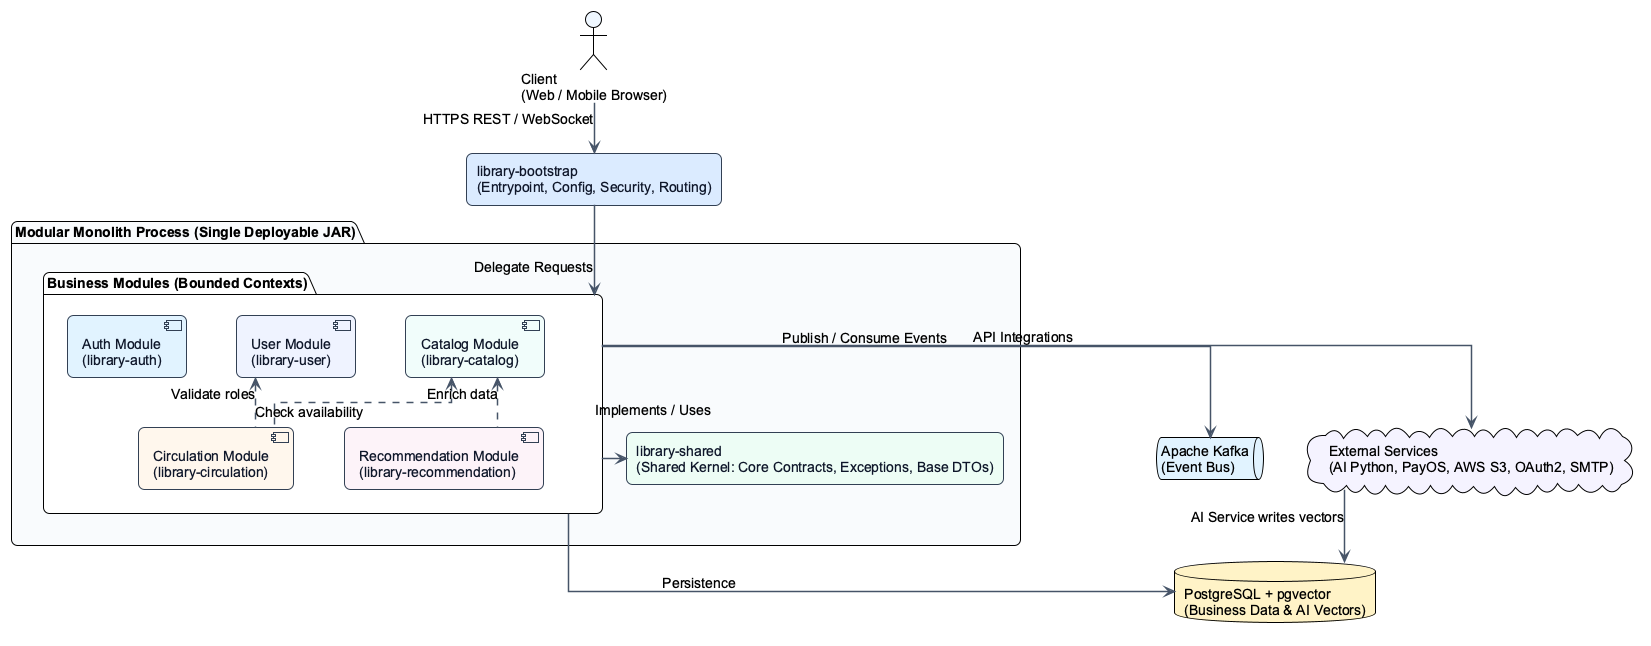
\includegraphics[width=\textwidth]{figures/ch06/backend/backend_architecture.png}
    \caption{Sơ đồ kiến trúc Modular Monolith tổng thể}
    \label{fig:be_architecture_diagram}
\end{figure}

Tương ứng với sơ đồ kiến trúc, mã nguồn vật lý cũng được tổ chức phân rã một cách chặt chẽ. Hình \ref{fig:be_folder_structure} thể hiện cấu trúc thư mục thực tế của dự án, minh chứng cho việc áp dụng triệt để mô hình Modular Monolith vào khâu triển khai mã nguồn.

\begin{figure}[H]
    \centering
    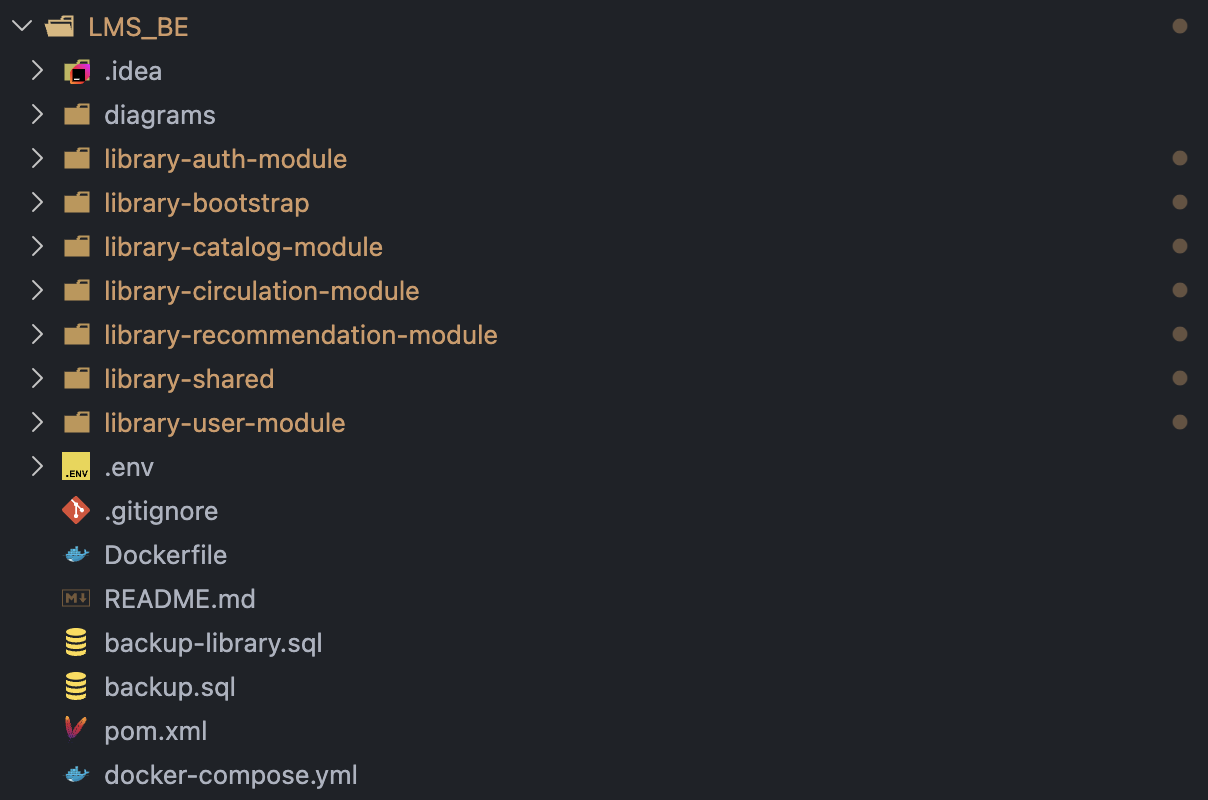
\includegraphics[width=0.45\textwidth]{figures/ch06/backend/backend_folder_tree.png}
    \caption{Cấu trúc thư mục mã nguồn Backend thực tế}
    \label{fig:be_folder_structure}
\end{figure}

Nhờ cấu trúc phân mảnh rõ ràng, toàn bộ các điểm cuối giao tiếp (API endpoints) của hệ thống đều được quy chuẩn hóa và tự động sinh tài liệu thông qua OpenAPI/Swagger. Do quy mô hệ thống lớn với hàng trăm API, Hình \ref{fig:be_swagger_publication} trích xuất giao diện API của module đại diện (Publication Controller) nhằm minh chứng cho mức độ chi tiết và tính chuẩn mực của các API Contract, đảm bảo sự minh bạch khi tích hợp với Frontend và AI Service.

\begin{figure}[H]
    \centering
    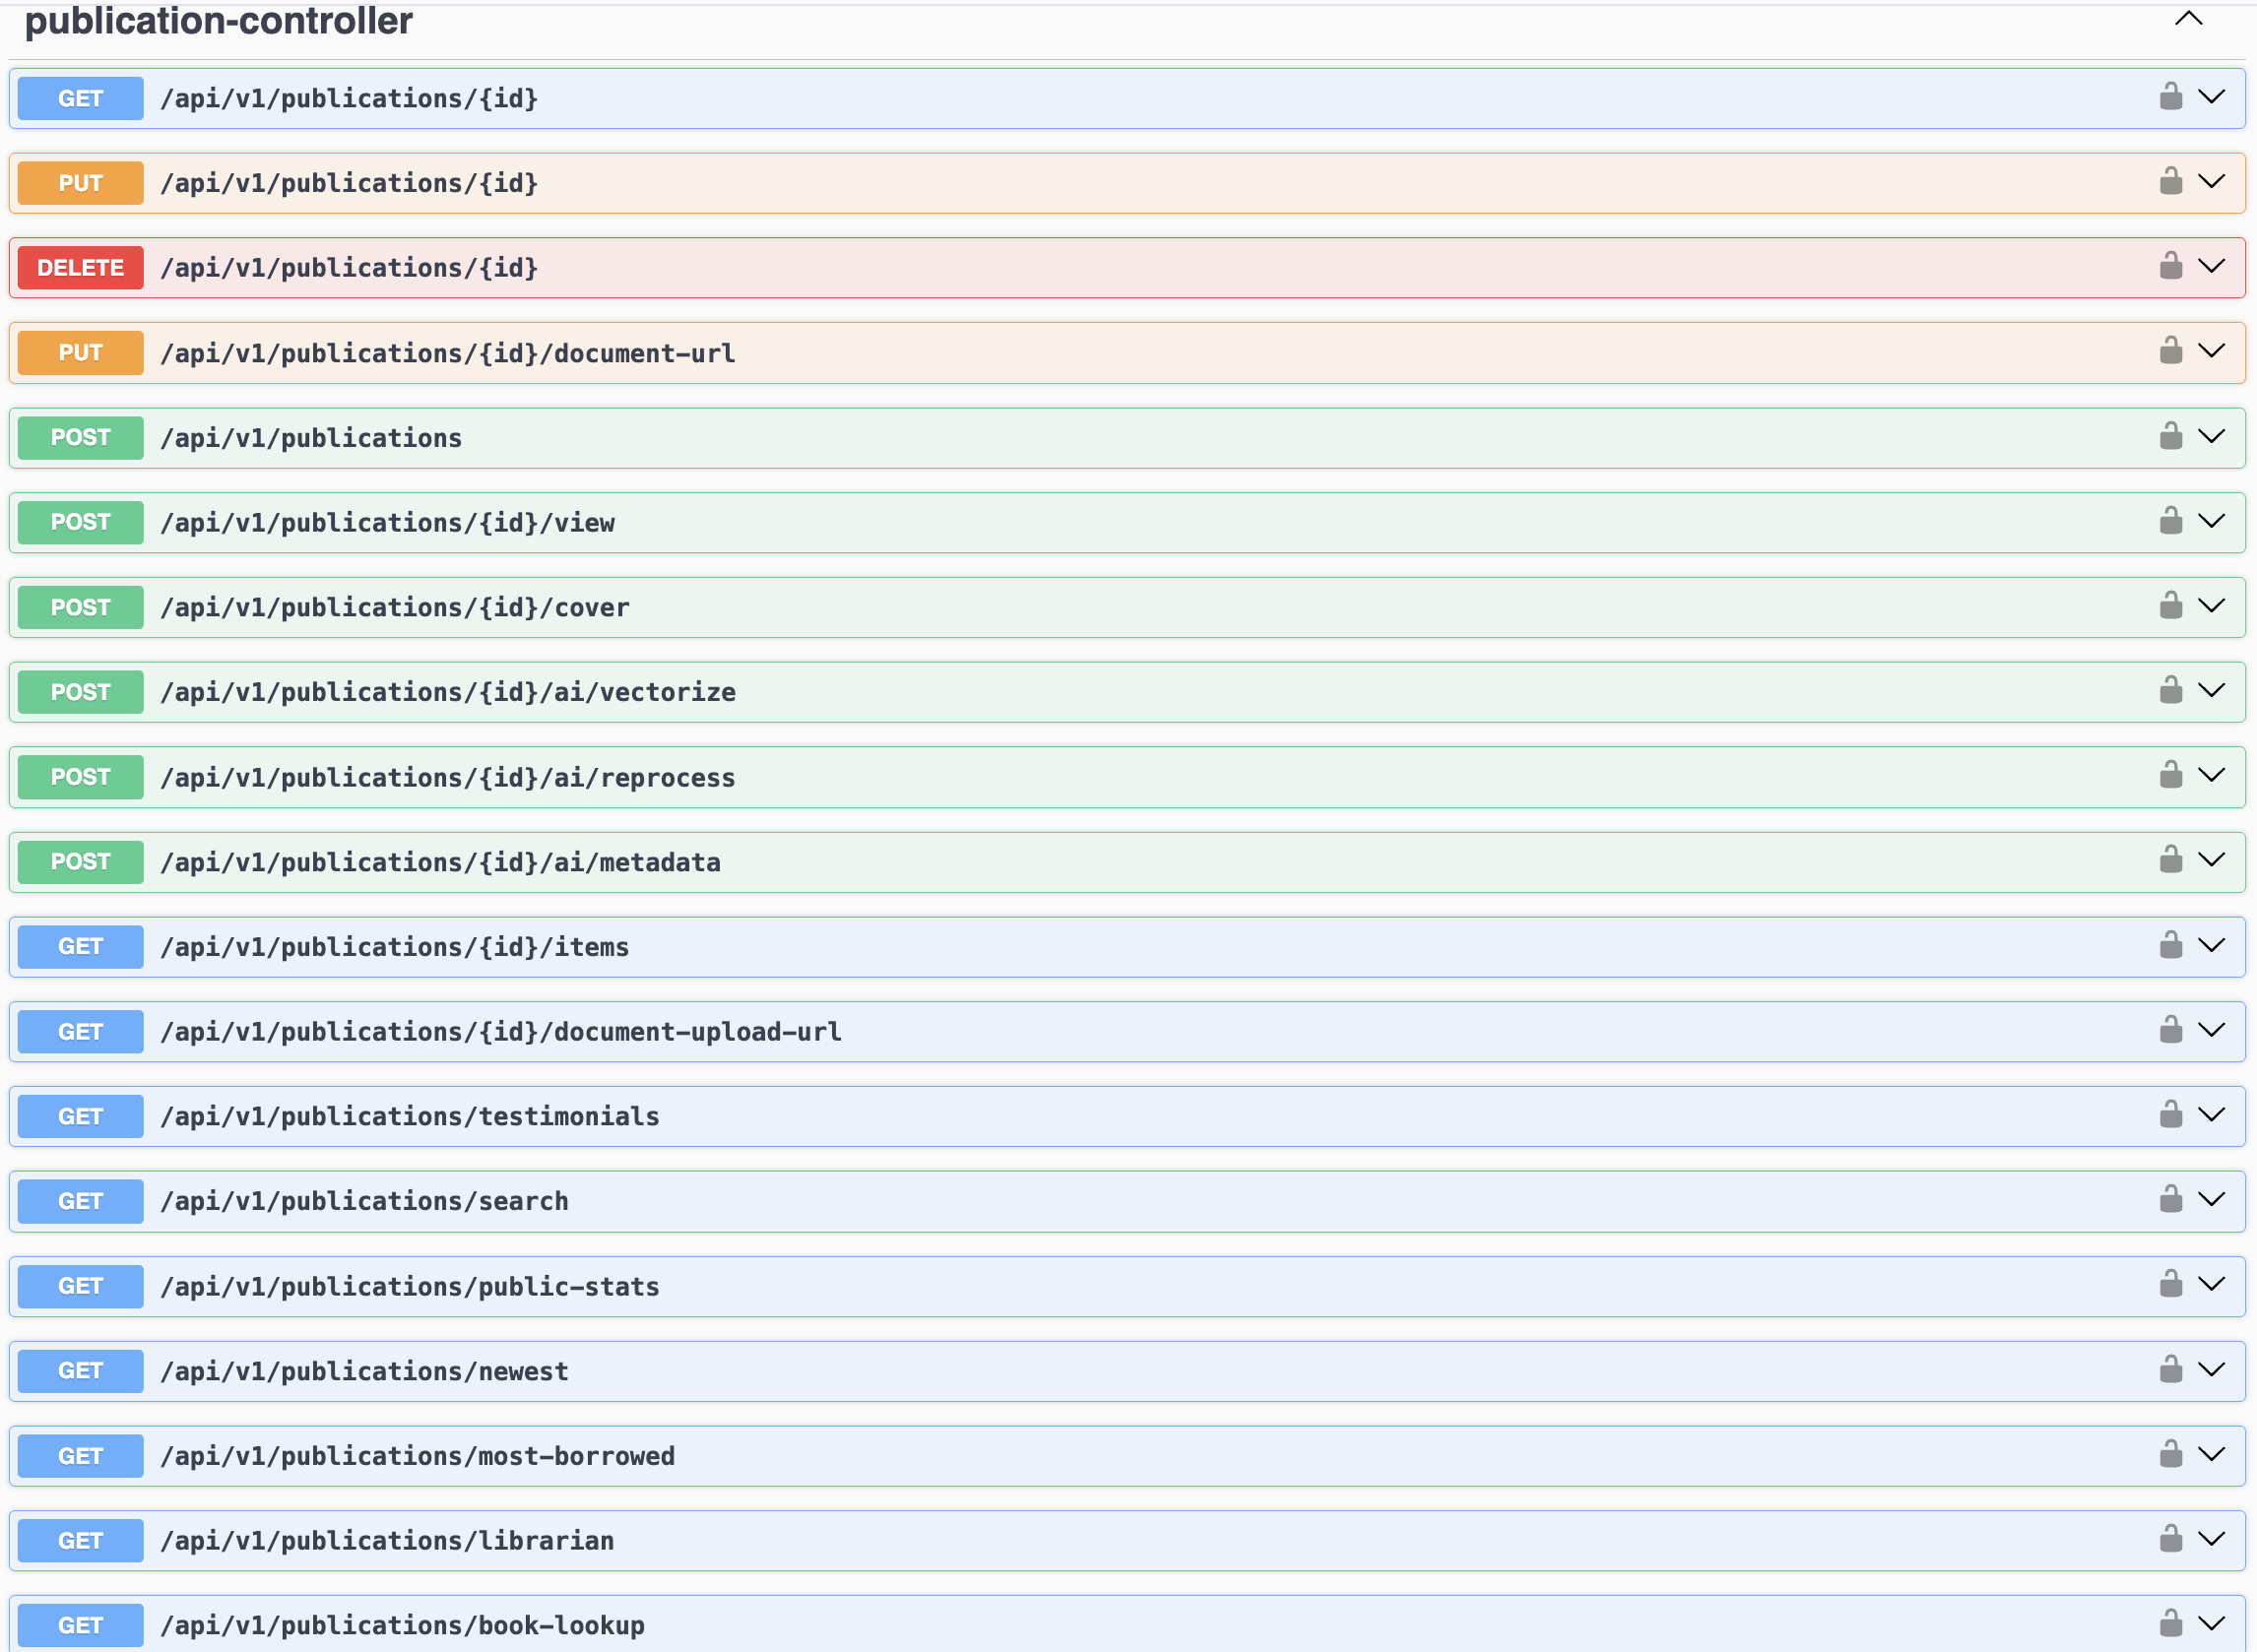
\includegraphics[width=0.85\linewidth]{figures/ch06/backend/publication-controller-swagger.png}
    \caption{Tài liệu hóa API tự động bằng Swagger (Đại diện module Publication)}
    \label{fig:be_swagger_publication}
\end{figure}

Chi tiết nhiệm vụ và nội dung hiện thực của toàn bộ các phân hệ con trong kiến trúc Backend được tổng hợp cụ thể tại Bảng \ref{tab:be_modules_implemented}.

% (Giữ nguyên Bảng \begin{longtable} của bạn ở bên dưới)

\begin{longtable}{|p{3.8cm}|p{4cm}|p{6.5cm}|}
\caption{Các module Backend đã hiện thực}
\label{tab:be_modules_implemented}\\
\hline
\textbf{Module} & \textbf{Nhóm chức năng} & \textbf{Nội dung đã hiện thực} \\
\hline
\endfirsthead
\hline
\textbf{Module} & \textbf{Nhóm chức năng} & \textbf{Nội dung đã hiện thực} \\
\hline
\endhead
\texttt{library-bootstrap} & Khởi động hệ thống &
Cấu hình Spring Boot, datasource, JPA, Flyway, Kafka, mail, OpenAPI, async,
security, CORS và biến môi trường triển khai. \\
\hline
\texttt{library-shared} & Thành phần dùng chung &
Response wrapper, exception, error code, base entity, DTO dùng chung, shared
port, Kafka event, S3 storage port và audit logging aspect. \\
\hline
\texttt{library-auth-module} & Xác thực &
Đăng ký, đăng nhập, refresh token, logout, xác thực email, quên mật khẩu, đặt
lại mật khẩu, Google OAuth2, JWT decoder và WebSocket authentication. \\
\hline
\texttt{library-user-module} & Người dùng và thông báo &
Hồ sơ người dùng, avatar, đổi mật khẩu, vai trò, trạng thái tài khoản, danh sách
notification, Kafka consumer và WebSocket push. \\
\hline
\texttt{library-admin-module} & Quản trị &
Quản lý tài khoản độc giả/thủ thư, tạo thủ thư, khóa/mở khóa, xác minh tài
khoản, cấu hình chính sách mượn trả và audit log. \\
\hline
\texttt{library-catalog-module} & Catalog thư viện &
Ấn phẩm, bản sao, tác giả, nhà xuất bản, danh mục, tag, tìm kiếm công khai,
chi tiết sách, trạng thái bản sao, upload bìa và presigned URL cho PDF. \\
\hline
\texttt{library-circulation-module} & Mượn--trả &
Yêu cầu mượn, mượn trực tiếp, xác nhận nhận sách, trả sách, đặt trước, hàng chờ,
gia hạn trạng thái, báo hư/mất và cập nhật trạng thái bản sao. \\
\hline
\texttt{library-circulation-module} & Phí phạt và scheduler &
Tính phí quá hạn/hư/mất, thanh toán tiền mặt, PayOS, nhắc sắp đến hạn, xử lý quá
hạn, hủy đặt trước hết hạn và dashboard vận hành. \\
\hline
\texttt{library-recommendation-module} & Tương tác bạn đọc &
Wishlist, lịch sử tìm kiếm, lượt xem, rating, comment, phản hồi rating của thủ
thư, đánh giá hệ thống và thống kê tương tác. \\
\hline
\texttt{library-recommendation-module} & AI Gateway &
Gọi semantic search, sách tương tự, recommendation, gửi yêu cầu xử lý PDF, nhận
AI callback có HMAC và cập nhật metadata AI về publication. \\
\hline
\end{longtable}

Để đảm bảo các miền nghiệp vụ nêu trên phối hợp nhịp nhàng và chịu tải tốt, toàn bộ hệ thống được xây dựng trên một bộ tiêu chuẩn kỹ thuật cốt lõi nghiêm ngặt. Bảng \ref{tab:be_technical_summary} trình bày chi tiết các giải pháp nền tảng đã được triển khai, bao gồm chuẩn hóa giao tiếp API, cơ chế bảo mật không trạng thái (stateless), quản trị cơ sở dữ liệu tập trung và các luồng xử lý tác vụ nền bất đồng bộ.

\begin{table}[H]
\centering
\small
\begin{tabularx}{\textwidth}{|p{3.6cm}|X|}
\hline
\textbf{Hạng mục Backend} & \textbf{Nội dung đã hiện thực} \\
\hline
Chuẩn API &
\texttt{ApiResponseApp}, \texttt{PageResponse}, mã lỗi nghiệp vụ, message theo
\texttt{Accept-Language}, \texttt{GlobalExceptionHandler}. \\
\hline
Bảo mật &
Spring Security stateless, JWT, refresh token, Google OAuth2, kiểm tra role bằng
annotation và AOP, khóa tài khoản có hiệu lực ngay khi đăng nhập. \\
\hline
Dữ liệu &
PostgreSQL, Flyway migration, entity audit, phân biệt ấn phẩm và bản sao, lưu
trạng thái giao dịch, fine, reservation, notification và dữ liệu AI. \\
\hline
Tác vụ nền &
Scheduler nhắc hạn, xử lý quá hạn, hủy reservation hết hạn, Kafka event cho
notification và async callback sang frontend. \\
\hline
Tích hợp ngoài &
S3-compatible storage, email SMTP, Google OAuth2, PayOS, AI service, WebSocket
và Swagger/OpenAPI. \\
\hline
Quan sát vận hành &
Audit log, dashboard thủ thư, dashboard admin, lỗi nghiệp vụ có mã rõ ràng và
log cho callback/tác vụ nền. \\
\hline
\end{tabularx}
\caption{Các hạng mục kỹ thuật Backend}
\label{tab:be_technical_summary}
\end{table}

% --- ĐOẠN CHUYỂN Ý 2: TỪ KỸ THUẬT SANG GIÁ TRỊ VẬN HÀNH ---
Việc áp dụng kiến trúc Modular Monolith và các công nghệ phụ trợ không chỉ nhằm mục đích đáp ứng yêu cầu phần mềm, mà còn trực tiếp giải quyết các bài toán vận hành thực tế của một thư viện hiện đại. Bảng \ref{tab:be_value_highlights} đúc kết những giá trị cốt lõi mà thiết kế Backend đã mang lại, từ việc đảm bảo tính toàn vẹn dữ liệu xuyên suốt các giao dịch mượn trả, khả năng bảo trì hệ thống, cho đến độ an toàn tuyệt đối khi giao tiếp với các dịch vụ bên ngoài (External Services).

\begin{table}[H]
\centering
\small
\begin{tabularx}{\textwidth}{|p{3.4cm}|X|p{3.4cm}|}
\hline
\textbf{Điểm hiện thực} & \textbf{Nội dung đã làm} & \textbf{Ý nghĩa vận hành} \\
\hline
Ranh giới module &
Auth, user, admin, catalog, circulation và recommendation tách theo miền nghiệp vụ. &
Dễ đọc code, dễ kiểm thử và giảm phụ thuộc chéo khi mở rộng. \\
\hline
Luồng trạng thái sách &
Backend kiểm soát item, transaction, reservation, fine và notification theo một nguồn dữ liệu thống nhất. &
Tránh lệch trạng thái giữa giao diện bạn đọc và giao diện thủ thư. \\
\hline
Tích hợp ngoài &
PayOS, Google OAuth2, email, storage, AI service, WebSocket và Swagger/OpenAPI. &
Hệ thống có khả năng chạy như một sản phẩm hoàn chỉnh, không chỉ là prototype. \\
\hline
An toàn callback &
Webhook PayOS và callback AI đều có cơ chế kiểm tra chữ ký hoặc token. &
Giảm rủi ro cập nhật trạng thái giả từ request bên ngoài. \\
\hline
\end{tabularx}
\caption{Các điểm giá trị nổi bật ở Backend}
\label{tab:be_value_highlights}
\end{table}

\subsection{Hiện thực AI Service}

AI service được tách thành một tiến trình Python riêng để xử lý các tác vụ có
đặc thù tính toán và phụ thuộc mô hình. Service này không quyết định nghiệp vụ
mượn--trả; nó chỉ sinh metadata, vector, điểm tương đồng hoặc danh sách mã ấn
phẩm. Backend luôn là nơi chuẩn hóa kết quả cuối cùng trước khi trả về frontend.

Để đáp ứng được đặc thù xử lý này, kiến trúc nội bộ của AI Service được phân tách thành luồng xử lý đồng bộ (Synchronous Gateway) và luồng xử lý nền bất đồng bộ (Background Worker). Hình \ref{fig:ai_architecture} mô tả bức tranh tổng thể về cách AI Service tương tác với các thành phần trong hệ thống: từ việc nhận yêu cầu từ Spring Boot, tải tài liệu vật lý từ AWS S3, cho đến việc giao tiếp với LLM (Google Gemini) để trích xuất tri thức. Đặc biệt, để đảm bảo tính toàn vẹn dữ liệu, mọi bản cập nhật trạng thái từ tiến trình xử lý nền (Worker) trả về Backend đều được ký xác thực bằng thuật toán mã hóa HMAC (Hash-based Message Authentication Code).

\begin{figure}[H]
    \centering
    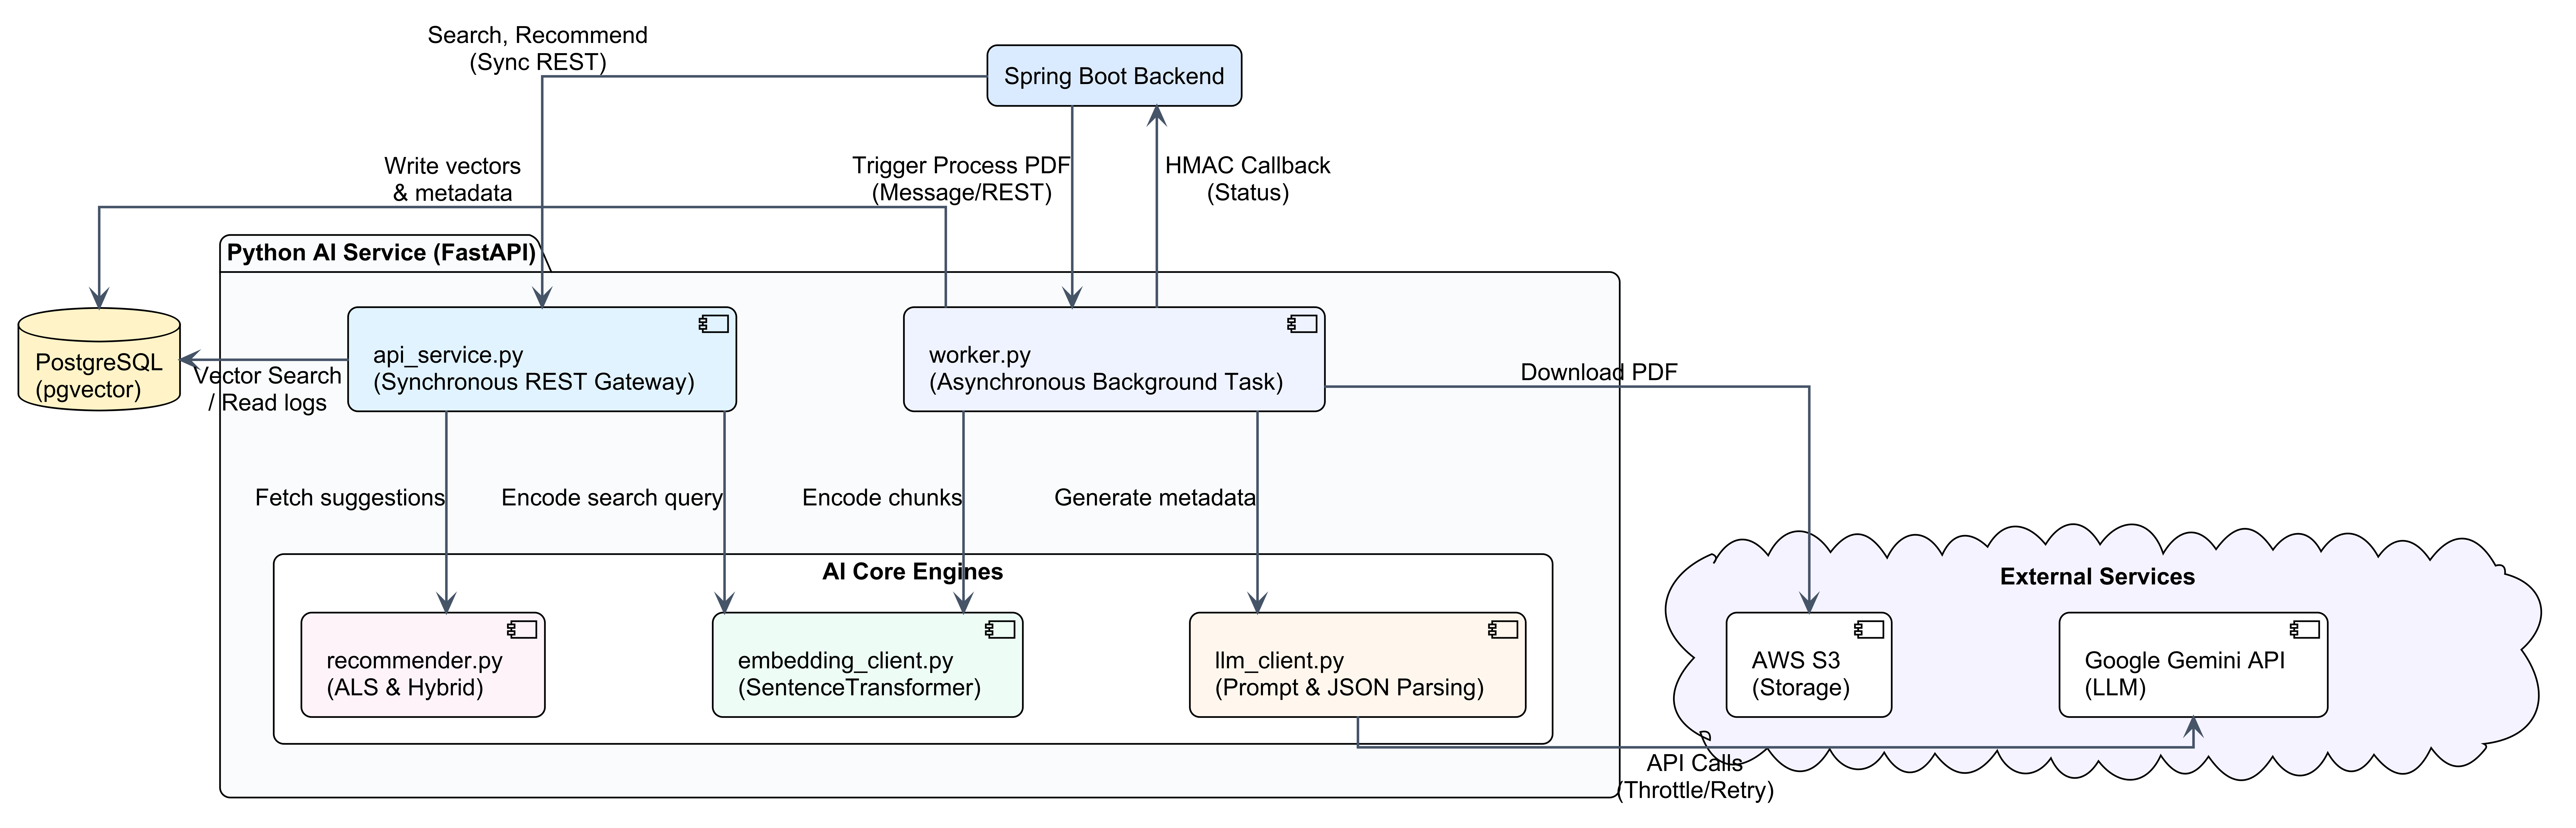
\includegraphics[width=\textwidth]{figures/ch06/ai/ai_architecture.png}
    \caption{Kiến trúc tổng thể và luồng giao tiếp của AI Service}
    \label{fig:ai_architecture}
\end{figure}

Lõi sức mạnh của phân hệ AI nằm ở luồng xử lý và số hóa tài liệu (ETL Pipeline). Khi một tài liệu PDF mới được hệ thống ghi nhận, tiến trình ETL (Hình \ref{fig:ai_etl_pipeline}) sẽ tự động được kích hoạt. Quá trình này trải qua nhiều công đoạn phức tạp: làm sạch nhiễu (Header/Footer), chia nhỏ văn bản bằng kỹ thuật Cửa sổ trượt (Sliding Window), sinh vector nhúng (Embedding) bằng mô hình SentenceTransformer tiếng Việt, và cuối cùng là đúc kết siêu dữ liệu (Tóm tắt, Phân loại độc giả, Gắn thẻ) thông qua LLM trước khi lưu trữ vào cơ sở dữ liệu \texttt{pgvector}.

\begin{figure}[H]
    \centering
    % Hạ tỷ lệ chiều rộng xuống để chiều cao tự động co ngắn lại vừa trang
    \includegraphics[width=0.52\textwidth]{figures/ch06/ai/ai_etl_pipeline.png}
    \caption{Luồng xử lý trích xuất, biến đổi và tải dữ liệu (ETL Pipeline) cho tài liệu PDF}
    \label{fig:ai_etl_pipeline}
\end{figure}

Chi tiết về chức năng và nhiệm vụ cụ thể của từng thành phần mã nguồn bên trong AI Service được thống kê tại Bảng \ref{tab:ai_components_implemented}.

% ================= NỐI TIẾP BẰNG BẢNG CỦA BẠN =================

\begin{longtable}{|p{3.8cm}|p{4cm}|p{6.5cm}|}
\caption{Các thành phần AI Service đã hiện thực}
\label{tab:ai_components_implemented}\\
\hline
\textbf{Thành phần} & \textbf{Nhóm chức năng} & \textbf{Nội dung đã hiện thực} \\
\hline
\endfirsthead
\hline
\textbf{Thành phần} & \textbf{Nhóm chức năng} & \textbf{Nội dung đã hiện thực} \\
\hline
\endhead
\texttt{api\_service.py} & FastAPI gateway &
Cung cấp health check, semantic search, similar publications, recommendation và
xử lý publication theo request đồng bộ. \\
\hline
\texttt{worker.py} & Xử lý nền &
Nhận message xử lý sách, tải PDF, chạy ETL, ghi trạng thái và gửi callback về
backend bằng chữ ký HMAC. \\
\hline
\texttt{pdf\_processing.py} & PDF ETL &
Tải/đọc PDF, trích xuất text bằng PyMuPDF, làm sạch header/footer/số trang, chia
chunk sliding window. \\
\hline
\texttt{pipeline.py} & Điều phối ETL &
Hash skip, sinh embedding, chọn chunk đại diện, reduce metadata bằng LLM, fallback
local khi lỗi và ghi kết quả vào database. \\
\hline
\texttt{embedding\_client.py} & Embedding &
Load SentenceTransformer tiếng Việt, sinh vector 768 chiều, normalize vector và
phục vụ semantic search/similar/recommendation. \\
\hline
\texttt{llm\_client.py} & Metadata AI &
Gọi Gemini, throttle/retry, ép output JSON, sinh summary, audience, tag tiếng
Việt và alias \texttt{tags\_en}. \\
\hline
\texttt{tag\_quality.py} & Làm sạch tag &
Lọc tag rác, chuẩn hóa alias Anh--Việt, map tag tiếng Việt sang thuật ngữ tiếng
Anh để hỗ trợ tìm kiếm song ngữ. \\
\hline
\texttt{recommender.py} & Gợi ý sách &
Huấn luyện ALS implicit feedback, kết hợp content-based, collaborative signal và
trending fallback. \\
\hline
\texttt{init\_schema.sql} & Dữ liệu AI &
Khởi tạo schema \texttt{ai\_engine}, bảng vector, ETL run, search log, index
pgvector và bảng recommendation. \\
\hline
\end{longtable}

% --- ĐOẠN CHUYỂN Ý 1: TỪ MODULE SANG MINH CHỨNG HÌNH ẢNH ---
Để minh chứng cho hoạt động của các thành phần mã nguồn nêu trên, hệ thống ghi nhận các kết quả đầu ra rõ rệt ở cả lớp giao diện người dùng lẫn lớp lưu trữ dữ liệu. Hình \ref{fig:ai_feature_showcase} thể hiện trải nghiệm trực quan của bạn đọc khi sử dụng công cụ tìm kiếm ngữ nghĩa và tiếp nhận các đề xuất sách cá nhân hóa. Song song đó, Hình \ref{fig:ai_etl_vector_showcase} cung cấp bằng chứng kỹ thuật (Technical Evidence) về tiến trình xử lý nền (ETL run) và cấu trúc dữ liệu vector nhiều chiều đã được lưu trữ thành công trong \texttt{pgvector}.

\begin{figure}[H]
    \centering
    \begin{subfigure}[b]{0.48\textwidth}
        \centering
        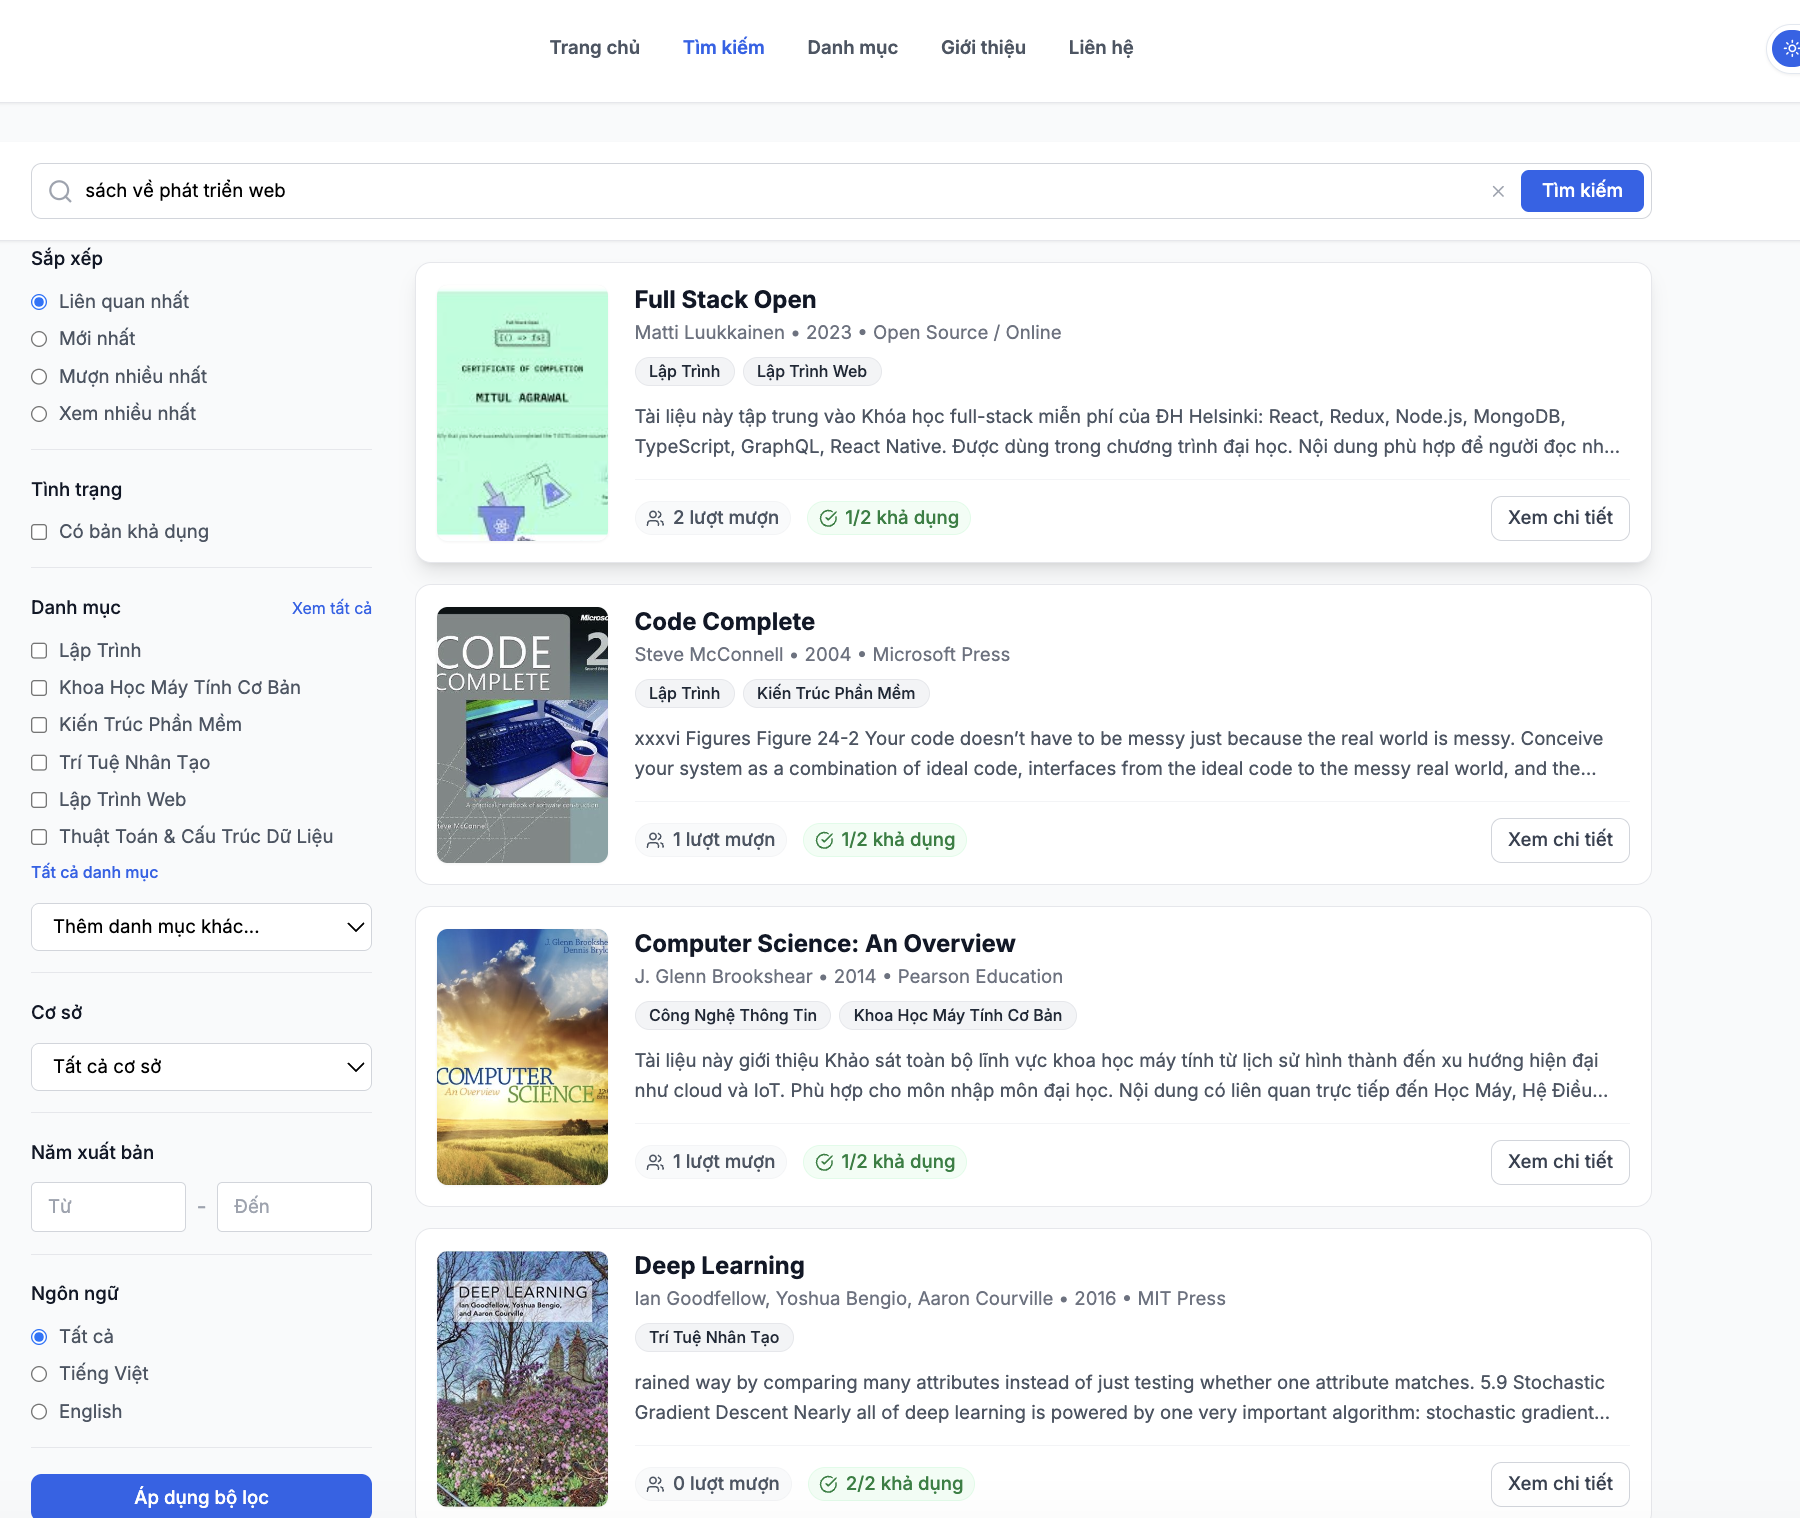
\includegraphics[width=\linewidth]{figures/ch06/ai/semantic_search.png}
        \caption{Semantic search}
    \end{subfigure}
    \hfill
    \begin{subfigure}[b]{0.48\textwidth}
        \centering
        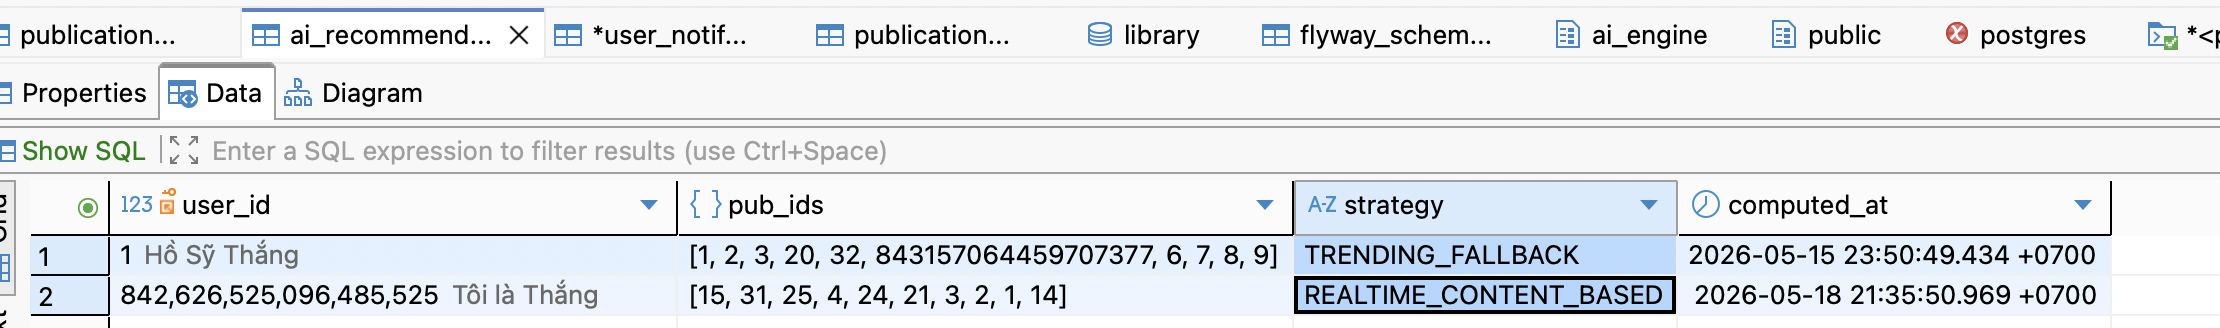
\includegraphics[width=\linewidth]{figures/ch06/ai/recommendation.png}
        \caption{Gợi ý sách}
    \end{subfigure}
    \caption{Các chức năng AI đã tích hợp vào hệ thống}
    \label{fig:ai_feature_showcase}
\end{figure}

\begin{figure}[H]
    \centering
    \begin{subfigure}[b]{0.48\textwidth}
        \centering
        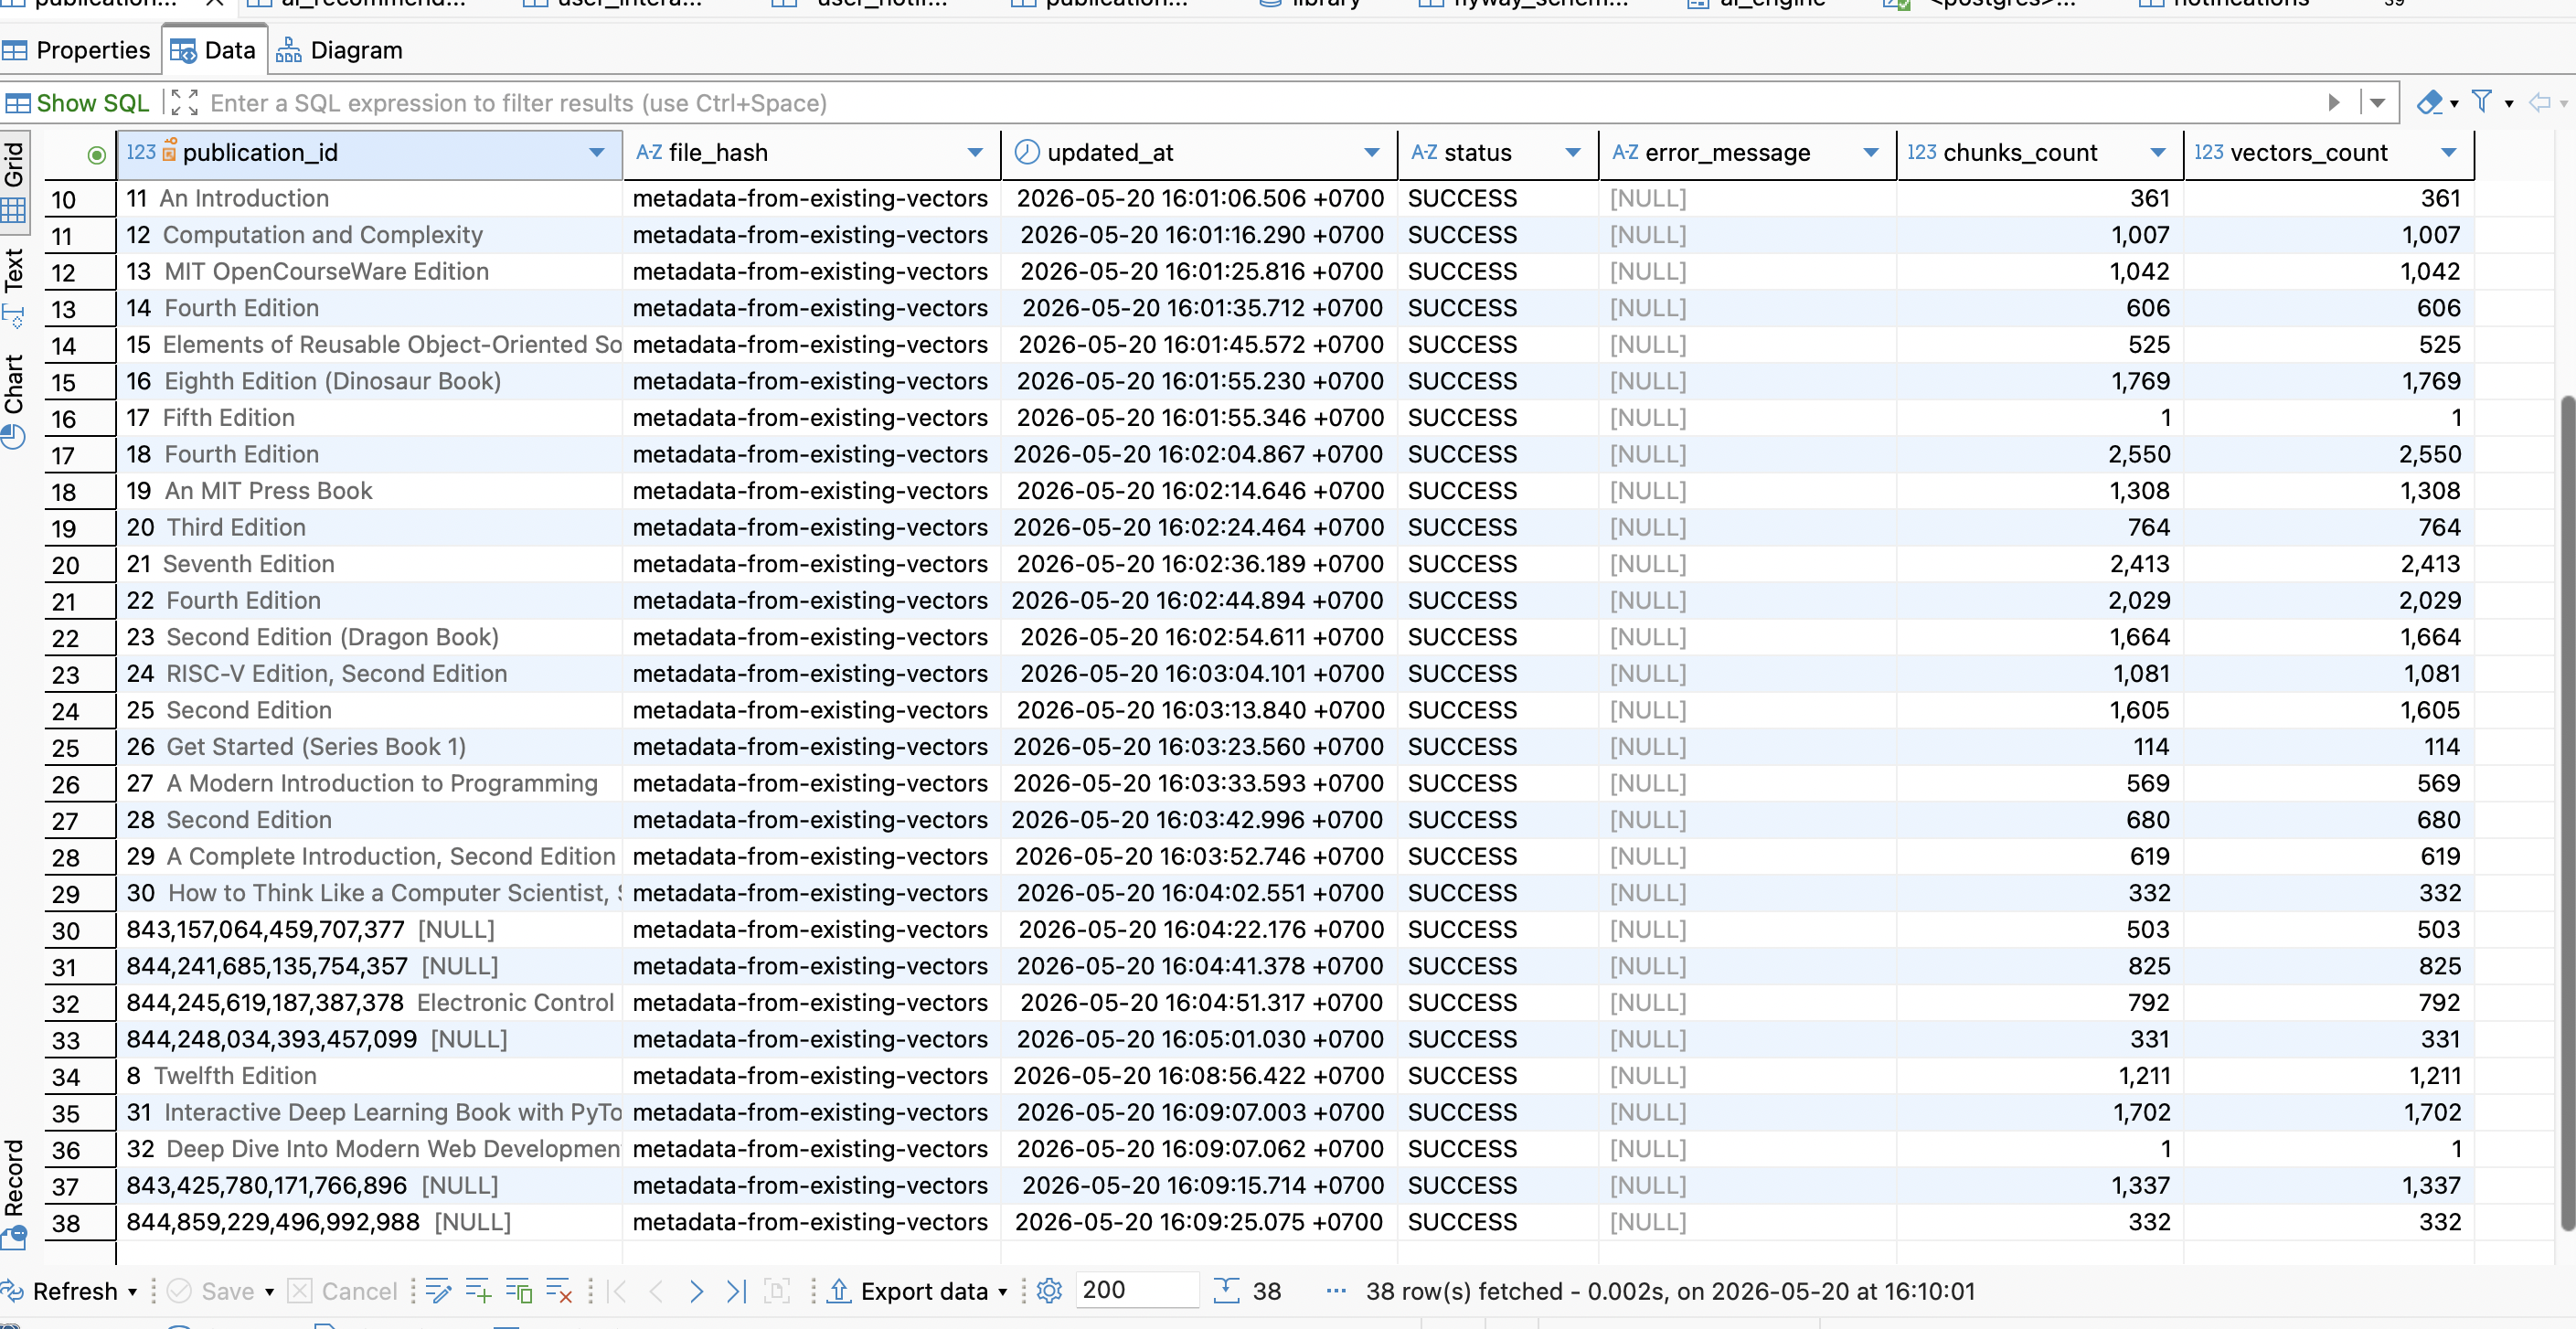
\includegraphics[width=\linewidth]{figures/ch06/ai/etl_run.png}
        \caption{Kết quả chạy ETL}
    \end{subfigure}
    \hfill
    \begin{subfigure}[b]{0.48\textwidth}
        \centering
        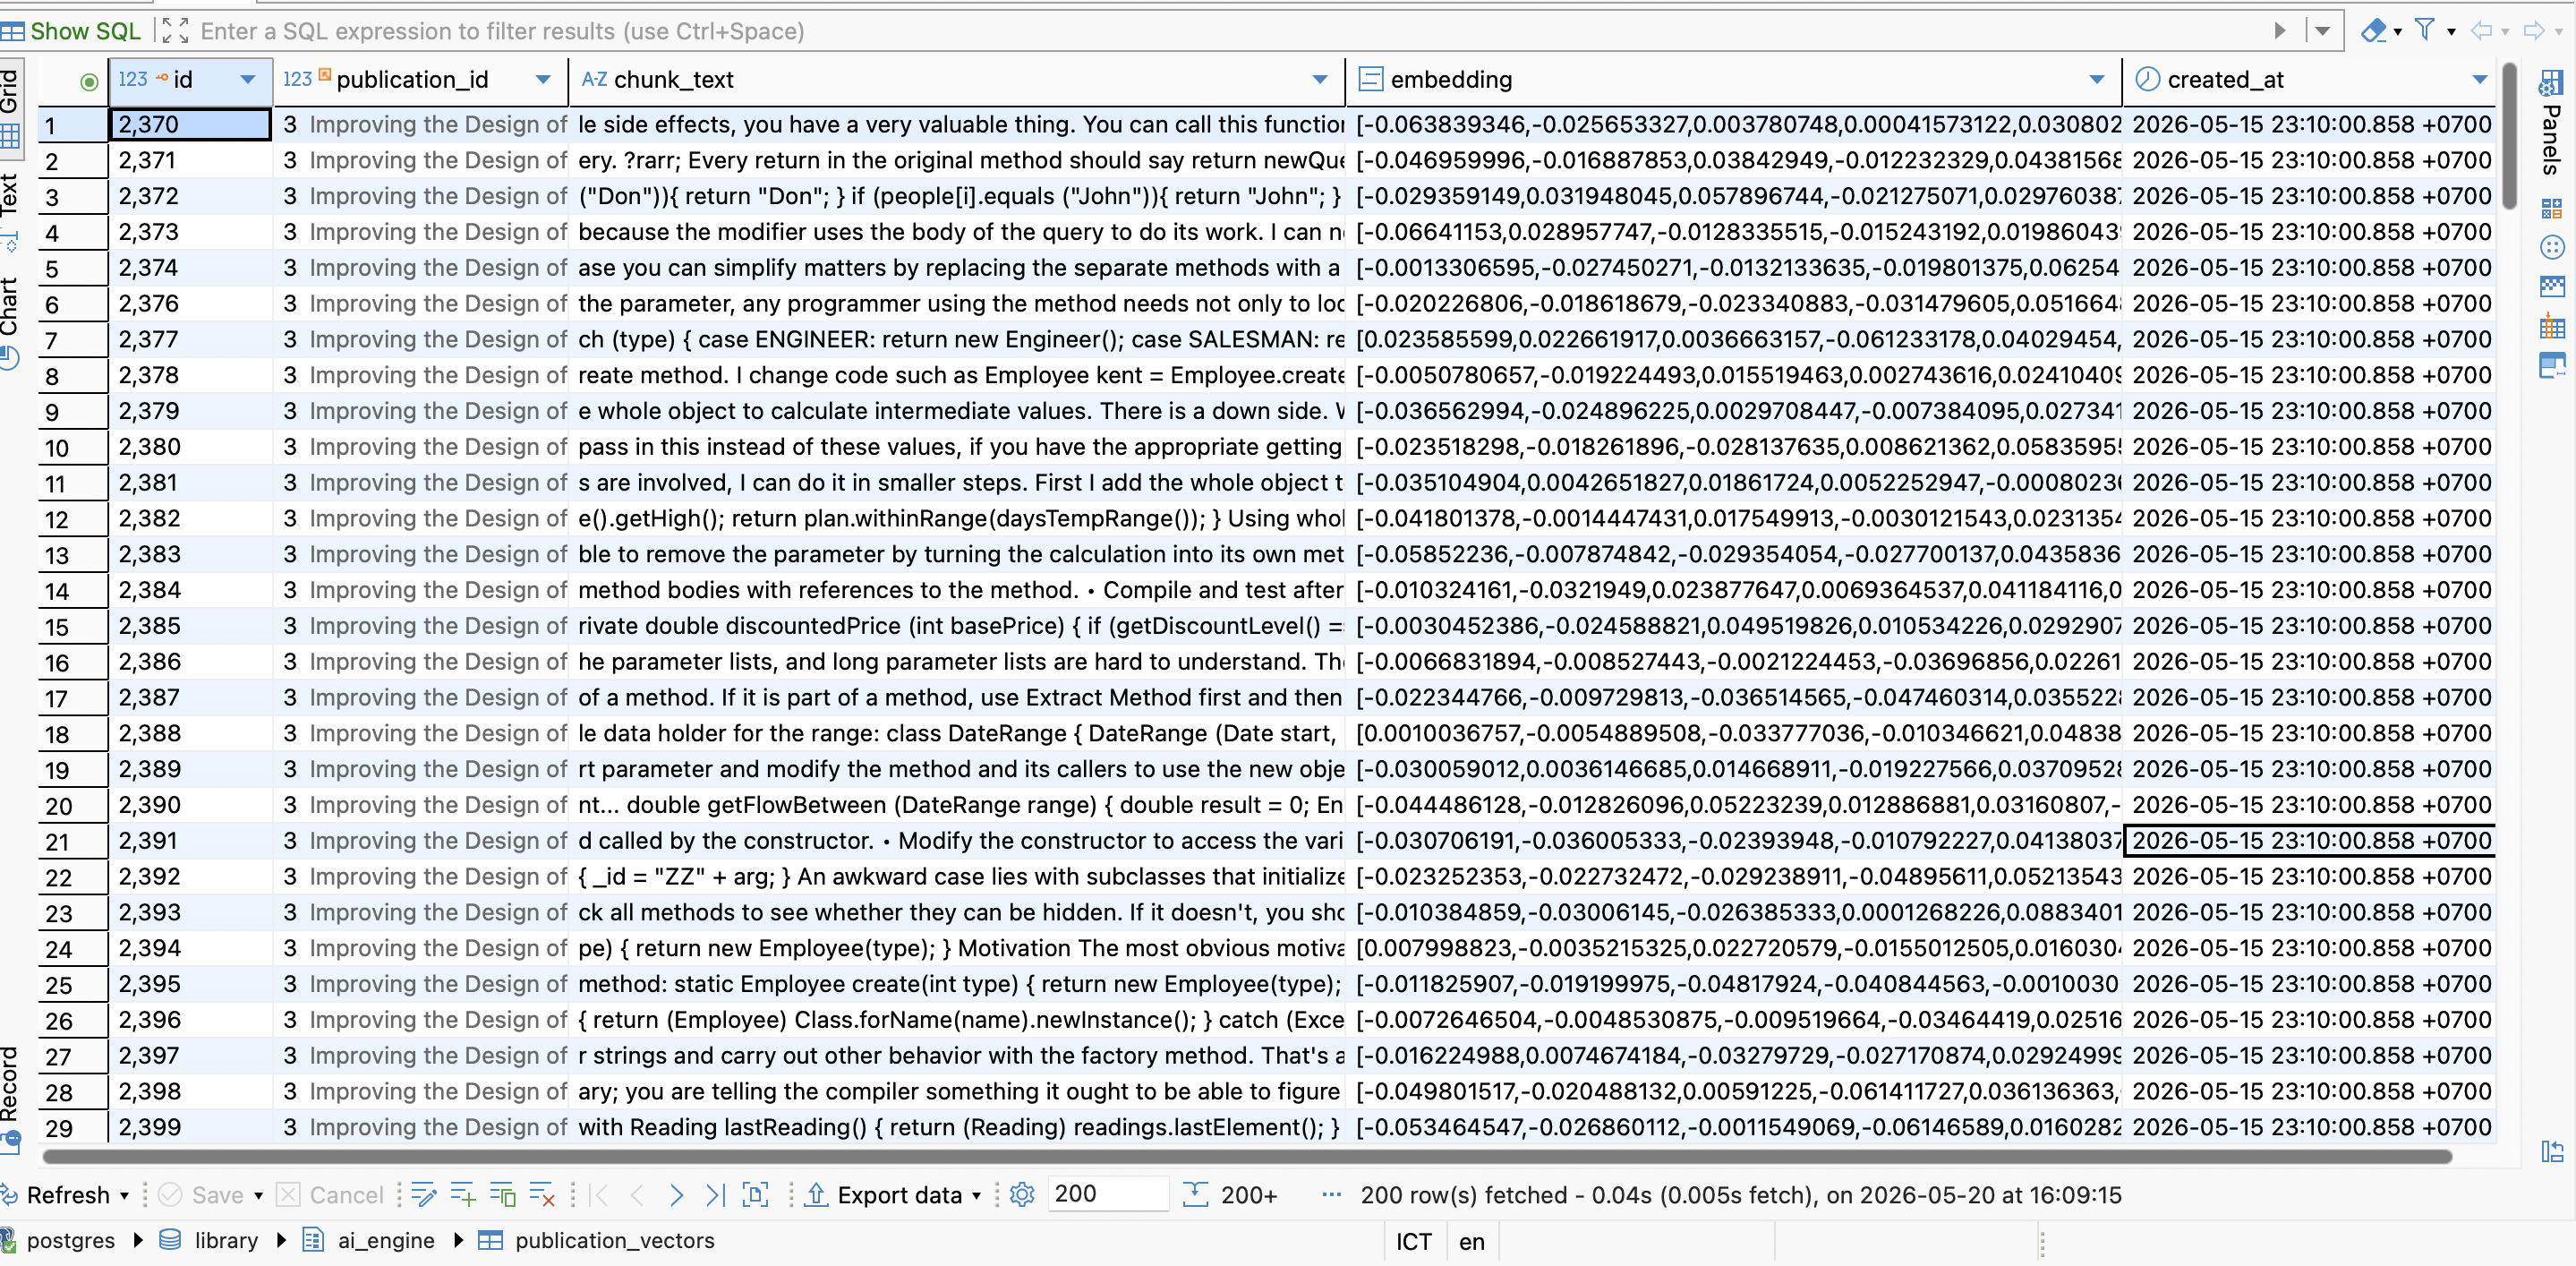
\includegraphics[width=\linewidth]{figures/ch06/ai/vector_db.png}
        \caption{Dữ liệu vector trong PostgreSQL}
    \end{subfigure}
    \caption{Pipeline xử lý PDF và lưu vector}
    \label{fig:ai_etl_vector_showcase}
\end{figure}

% --- ĐOẠN CHUYỂN Ý 2: TỪ HÌNH ẢNH SANG NĂNG LỰC KỸ THUẬT ---
Dựa trên các kết quả trực quan này, Bảng \ref{tab:ai_capability_summary} tổng hợp chi tiết các năng lực trí tuệ nhân tạo cốt lõi mà phân hệ AI Service đã đảm nhiệm. Các năng lực này được thiết kế không chỉ để phô diễn công nghệ, mà còn phải đáp ứng nghiêm ngặt các tiêu chuẩn về an toàn tích hợp, khả năng chịu lỗi (fault tolerance) và cơ chế dự phòng (fallback) khi giao tiếp với mô hình ngôn ngữ lớn (LLM).

\begin{table}[H]
\centering
\small
\begin{tabularx}{\textwidth}{|p{3.5cm}|X|}
\hline
\textbf{Năng lực AI} & \textbf{Nội dung đã hiện thực} \\
\hline
Xử lý PDF &
Upload PDF từ thủ thư, chạy ETL nền, lưu trạng thái \texttt{RUNNING},
\texttt{SUCCESS}, \texttt{FAILED}, không làm gián đoạn nghiệp vụ catalog. \\
\hline
Semantic search &
Sinh embedding cho truy vấn, tìm chunk gần nhất bằng pgvector, gom về
publication id và trả kết quả cho backend lọc nghiệp vụ. \\
\hline
Metadata enrichment &
Sinh summary, audience, tag học thuật, alias tiếng Anh và ghi về publication để
hiển thị trên chi tiết sách/tìm kiếm. \\
\hline
Similar books &
Tính tương đồng dựa trên vector nội dung và metadata để đề xuất sách liên quan
từ trang chi tiết. \\
\hline
Recommendation &
Gợi ý cá nhân hóa theo lịch sử xem, wishlist, mượn, rating; có fallback khi
người dùng mới hoặc dữ liệu tương tác còn ít. \\
\hline
An toàn tích hợp &
Callback HMAC, timeout/retry, fallback local khi LLM lỗi, kiểm thử API contract
và kiểm tra độ trễ cơ bản. \\
\hline
\end{tabularx}
\caption{Các năng lực AI đã tích hợp vào hệ thống}
\label{tab:ai_capability_summary}
\end{table}

% --- ĐOẠN CHUYỂN Ý 3: TỪ KỸ THUẬT SANG GIÁ TRỊ VẬN HÀNH ---
Công nghệ chỉ thực sự có ý nghĩa khi nó phục vụ đúng bài toán con người. Bảng \ref{tab:ai_value_highlights} đúc kết những điểm sáng nổi bật nhất, minh chứng cho việc ứng dụng AI đã thực sự giải phóng sức lao động của thủ thư (thông qua tự động hóa xử lý nền) và nâng tầm trải nghiệm khám phá tri thức của độc giả (thông qua tìm kiếm trên lõi nội dung thay vì từ khóa bề mặt).

\begin{table}[H]
\centering
\small
\begin{tabularx}{\textwidth}{|p{3.4cm}|X|p{3.4cm}|}
\hline
\textbf{Điểm hiện thực} & \textbf{Nội dung đã làm} & \textbf{Giá trị thực tế} \\
\hline
Xử lý nền &
AI worker nhận request, tải PDF, chạy ETL và callback kết quả về backend. &
Thủ thư không phải chờ AI xử lý xong mới tiếp tục thao tác catalog. \\
\hline
Tìm trên nội dung PDF &
Chunk nội dung được embedding và lưu vào pgvector để semantic search. &
Kết quả tìm kiếm dựa trên nội dung sách, không chỉ tiêu đề hoặc mô tả. \\
\hline
Metadata enrichment &
Sinh summary, audience, tag tiếng Việt và alias tiếng Anh. &
Trang chi tiết sách và bộ lọc tìm kiếm có thêm dữ liệu có ích cho người đọc. \\
\hline
Fallback &
Khi LLM lỗi hoặc dữ liệu tương tác ít, hệ thống dùng rule local, content-based và trending. &
Tính năng AI vẫn có kết quả ổn định trong điều kiện demo hoặc quota giới hạn. \\
\hline
\end{tabularx}
\caption{Các điểm giá trị nổi bật ở AI Service}
\label{tab:ai_value_highlights}
\end{table}

% --- ĐOẠN CHUYỂN Ý 4: TỔNG KẾT TOÀN BỘ CHƯƠNG 6 ---
\subsection{Tổng kết kết quả hiện thực}

Khép lại toàn bộ quá trình triển khai từ Frontend, Backend đến AI Service, sự thành công của một hệ thống phần mềm không chỉ nằm ở việc hoàn thiện từng module đơn lẻ, mà là khả năng liên kết chúng thành các luồng nghiệp vụ (Business Flows) thông suốt.

Bảng \ref{tab:implementation_value_flows} tổng hợp 4 luồng giá trị xương sống của dự án, đối chiếu trực tiếp giữa các thành phần công nghệ đã tham gia và những minh chứng rõ nét đã được trình bày xuyên suốt chương này. Đây là thước đo cuối cùng khẳng định hệ thống đã được xây dựng hoàn chỉnh từ đầu đến cuối (end-to-end) và đáp ứng trọn vẹn bài toán thực tiễn đặt ra ban đầu.

\begin{table}[H]
\centering
\small
\begin{tabularx}{\textwidth}{|p{3.4cm}|X|p{3.4cm}|}
\hline
\textbf{Luồng được show} & \textbf{Thành phần tham gia} & \textbf{Kết quả thể hiện trong Chương 6} \\
\hline
Upload và xử lý sách &
Frontend upload, Backend catalog/AI gateway, AI worker, pgvector. &
Có màn hình upload, bảng module, ảnh ETL, ảnh vector DB và callback. \\
\hline
Tìm kiếm thông minh &
Public search UI, Backend search API, AI semantic search, catalog filter. &
Có màn hình tìm kiếm, bảng năng lực AI và ảnh semantic search. \\
\hline
Mượn--trả và thanh toán &
User/librarian UI, circulation module, PayOS, notification realtime. &
Có màn hình dashboard, mượn sách, QR PayOS, cập nhật thanh toán và notification. \\
\hline
Quản trị vận hành &
Admin/librarian pages, audit/policy, scheduler, API documentation. &
Có bảng module Backend, bảng giá trị Backend và ảnh Swagger/cấu trúc module. \\
\hline
\end{tabularx}
\caption{Các luồng giá trị được minh chứng trong phần hiện thực}
\label{tab:implementation_value_flows}
\end{table}

\section{Tổng kết hiện thực}

Về tổng thể, nhóm đã hiện thực hệ thống theo đúng ba lớp: frontend phục vụ tương
tác theo vai trò, backend giữ nghiệp vụ và dữ liệu gốc, AI service xử lý các tác
vụ thông minh. Các chức năng đã làm không chỉ dừng ở demo giao diện, mà đã nối
tới API, cơ sở dữ liệu, tác vụ nền, dịch vụ ngoài, kiểm thử và cấu hình triển
khai. Bảng dưới đây tóm tắt các luồng end-to-end quan trọng nhất.

\begin{table}[H]
\centering
\small
\begin{tabularx}{\textwidth}{|p{3.7cm}|X|}
\hline
\textbf{Luồng end-to-end} & \textbf{Các phần đã nối thông} \\
\hline
Đăng ký/đăng nhập &
Frontend auth pages, backend auth module, email verification, JWT/refresh token,
Google OAuth2 và route guard theo role. \\
\hline
Tra cứu và mượn sách &
Public/user search, catalog API, trạng thái bản sao, circulation API, thông báo
cho bạn đọc và dashboard thủ thư. \\
\hline
Đặt trước &
User reservation page, backend reservation queue, scheduler deadline, xác nhận
nhận sách và notification realtime. \\
\hline
Phí phạt &
Fine API, giao diện bạn đọc/thủ thư, PayOS QR, thanh toán tiền mặt, cập nhật
trạng thái fine và lịch sử giao dịch. \\
\hline
Upload PDF và AI &
Librarian upload, presigned URL, backend AI gateway, worker ETL, Gemini metadata,
pgvector và callback cập nhật publication. \\
\hline
Tìm kiếm/gợi ý thông minh &
Semantic search UI, AI service, recommendation module, behavior tracking, similar
books và fallback khi dữ liệu ít. \\
\hline
Vận hành &
Admin policy, audit log, scheduler, WebSocket notification, Docker Compose,
Nginx reverse proxy và cấu hình môi trường production. \\
\hline
\end{tabularx}
\caption{Các luồng end-to-end đã hiện thực}
\label{tab:end_to_end_summary}
\end{table}

\chapter{Kiểm thử phần mềm}

\section{Kiểm thử Frontend}

Nhóm đã kiểm thử frontend ở mức unit, context, component và service contract
bằng Jest, Testing Library và môi trường \texttt{jsdom}. Mục tiêu của phần kiểm
thử này là bắt các lỗi dễ tái xuất hiện trong giao diện: ánh xạ lỗi nghiệp vụ từ
backend sang thông báo người dùng, trạng thái đăng nhập, đa ngôn ngữ Việt--Anh,
light/dark/system theme, upload panel, nội dung notification, Google Maps ở
trang liên hệ, service layer gọi đúng endpoint, admin audit/policy contract và
các helper xử lý trạng thái đặt trước.

Khác với kiểm thử thủ công chỉ quan sát giao diện, các test này kiểm tra trực
tiếp logic dùng chung trong \texttt{utils} và \texttt{contexts}. Đây là những
vị trí có phạm vi ảnh hưởng rộng: nếu \texttt{LanguageContext} sai, nhiều trang
bị sai ngôn ngữ; nếu \texttt{ThemeContext} sai, toàn bộ SPA bị lệch theme; nếu
\texttt{getFriendlyErrorMessage} sai, cùng một lỗi backend có thể bị hiển thị
thành thông báo không đúng nghiệp vụ. Ngoài ra, các test service contract giúp
nhóm kiểm soát URL, query string và payload gửi về backend/AI service trước khi
chạy tích hợp thật.

\subsection{Môi trường và cấu hình kiểm thử}

Frontend dùng \texttt{jest.config.cjs} để chạy các file
\texttt{*.test.ts} và \texttt{*.test.tsx}. Môi trường \texttt{jsdom} được chọn
vì các context cần thao tác với \texttt{localStorage}, \texttt{document.html},
\texttt{matchMedia} và DOM giống trình duyệt. File \texttt{src/test/setup.ts}
nạp \texttt{@testing-library/jest-dom} để assertion có thể viết gần với hành vi
giao diện hơn, ví dụ \texttt{toHaveTextContent} và \texttt{toHaveClass}.

\begin{table}[H]
\centering
\small
\begin{tabularx}{\textwidth}{|p{3.5cm}|X|}
\hline
\textbf{Thành phần} & \textbf{Cấu hình sử dụng} \\
\hline
Test runner & Jest, chạy bằng script \texttt{npm test -- --runInBand}. \\
\hline
Biên dịch test & \texttt{ts-jest} với JSX mode \texttt{react-jsx}. \\
\hline
Môi trường DOM & \texttt{jest-environment-jsdom}, hỗ trợ kiểm tra DOM, \texttt{localStorage} và \texttt{document}. \\
\hline
Assertion UI & \texttt{@testing-library/jest-dom}. \\
\hline
Mock style & \texttt{identity-obj-proxy} cho file CSS/SCSS. \\
\hline
Alias import & \texttt{@/(.*)} trỏ về thư mục gốc frontend. \\
\hline
\end{tabularx}
\caption{Cấu hình kiểm thử Frontend}
\label{tab:fe_test_env}
\end{table}


\subsection{Phạm vi test đã hiện thực}

Nhóm ưu tiên các phần logic có khả năng ảnh hưởng nhiều màn hình thay vì chỉ
kiểm từng nút bấm riêng lẻ. Bộ test cuối cùng bao phủ 11 suite, gồm logic dùng
chung, context toàn cục, component nhỏ, trang liên hệ và service layer.

\begin{table}[H]
\centering
\scriptsize
\begin{tabularx}{\textwidth}{|p{5.1cm}|X|p{1.5cm}|}
\hline
\textbf{File test} & \textbf{Nội dung kiểm thử} & \textbf{Số test} \\
\hline
\begin{tabular}[c]{@{}l@{}}\texttt{src/utils/}\\\texttt{errorMessages.test.ts}\end{tabular} &
Ánh xạ mã lỗi backend sang thông báo phù hợp cho duplicate email, duplicate review và text lỗi chung. & 4 \\
\hline
\begin{tabular}[c]{@{}l@{}}\texttt{src/utils/}\\\texttt{notification}\\\texttt{Localization.test.ts}\end{tabular} &
Localize notification theo ngôn ngữ, giữ dữ liệu động như tên sách, số tiền và vị trí hàng chờ. & 3 \\
\hline
\begin{tabular}[c]{@{}l@{}}\texttt{src/utils/}\\\texttt{reservationUtils.test.ts}\end{tabular} &
Nhãn/màu trạng thái đặt trước, format ngày, quyền hủy reservation và deadline nhận sách. & 18 \\
\hline
\begin{tabular}[c]{@{}l@{}}\texttt{src/contexts/}\\\texttt{LanguageContext}\\\texttt{.test.tsx}\end{tabular} &
Ngôn ngữ mặc định, fallback text, chuyển sang English, lưu \texttt{localStorage} và cập nhật \texttt{document.lang}. & 2 \\
\hline
\begin{tabular}[c]{@{}l@{}}\texttt{src/contexts/}\\\texttt{ThemeContext}\\\texttt{.test.tsx}\end{tabular} &
Theme mặc định \texttt{system}, dark/light mode, \texttt{prefers-color-scheme}, class \texttt{dark} trên thẻ \texttt{html}. & 3 \\
\hline
\begin{tabular}[c]{@{}l@{}}\texttt{src/contexts/}\\\texttt{AuthContext.test.tsx}\end{tabular} &
Load role đã lưu, login bằng mật khẩu/social, parse role từ JWT và logout xóa token. & 5 \\
\hline
\begin{tabular}[c]{@{}l@{}}\texttt{src/contexts/}\\\texttt{UploadContext}\\\texttt{.test.tsx}\end{tabular} &
Thêm/cập nhật/xóa upload, progress/status và cảnh báo \texttt{beforeunload} khi upload đang chạy. & 5 \\
\hline
\begin{tabular}[c]{@{}l@{}}\texttt{src/components/}\\\texttt{UiComponents.test.tsx}\end{tabular} &
Star rating, password visibility toggle và disabled button. & 3 \\
\hline
\begin{tabular}[c]{@{}l@{}}\texttt{src/components/}\\\texttt{Switchers.test.tsx}\end{tabular} &
Language switcher và theme mode toggle thao tác đúng context toàn cục. & 2 \\
\hline
\begin{tabular}[c]{@{}l@{}}\texttt{src/pages/}\\\texttt{ContactPage.test.tsx}\end{tabular} &
Thông tin liên hệ, iframe Google Maps lazy loading và submit form liên hệ. & 2 \\
\hline
\begin{tabular}[c]{@{}l@{}}\texttt{src/api/}\\\texttt{frontendServices.test.ts}\end{tabular} &
Hợp đồng endpoint/payload cho search, semantic search, PayOS, wishlist, S3 upload, rating, admin audit, circulation policy, system review và ghi chú giao dịch. & 10 \\
\hline
\textbf{Tổng cộng} & \textbf{11 test suites} & \textbf{58} \\
\hline
\end{tabularx}
\caption{Các file test Frontend đã hiện thực}
\label{tab:fe_test_files}
\end{table}


\begin{figure}[H]
    \centering
    \IfFileExists{figures/ch07/test-results/fe-jest-result.png}{
        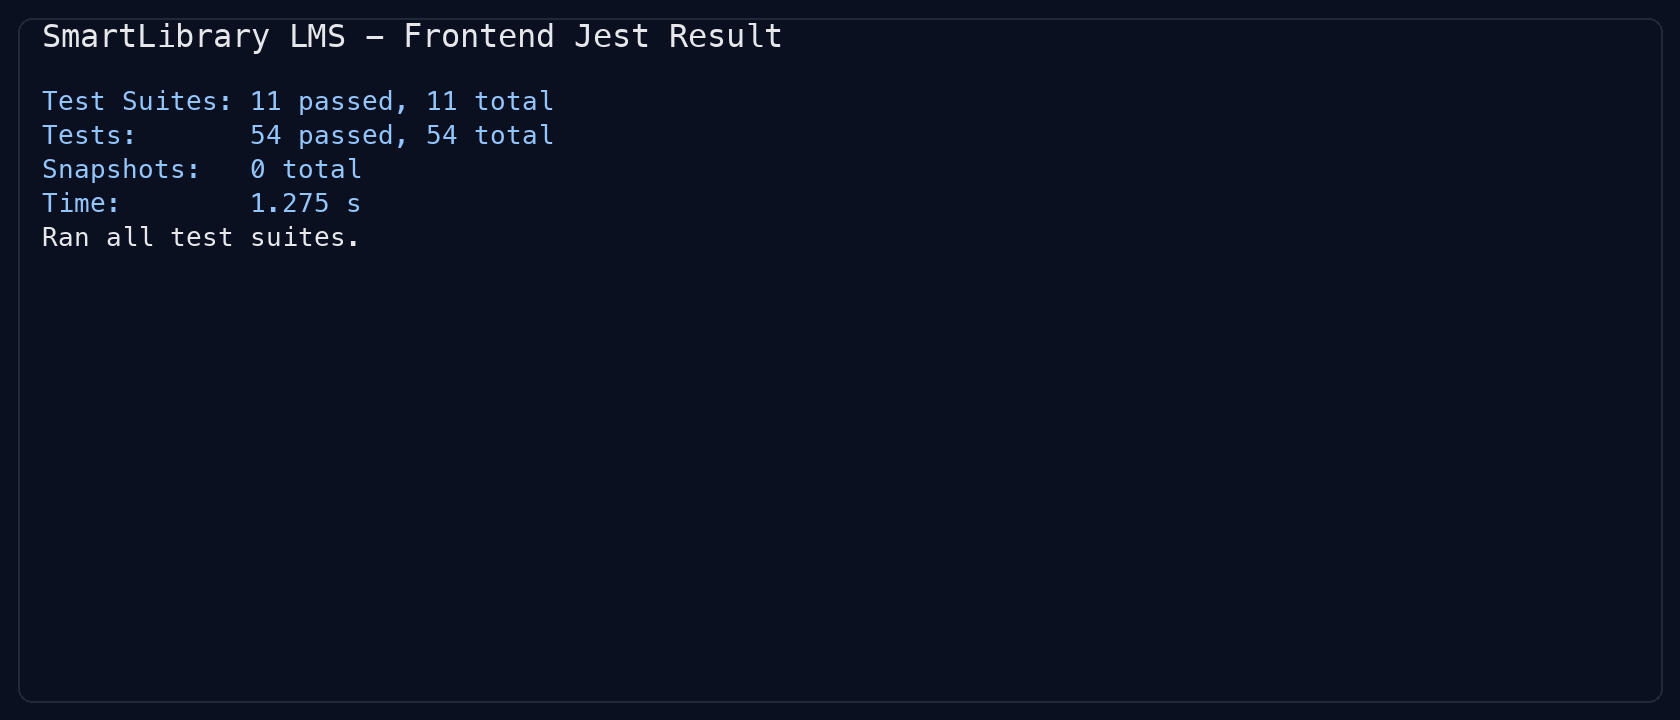
\includegraphics[width=0.9\textwidth]{figures/ch07/test-results/fe-jest-result.png}
    }{
        \fbox{\parbox[c][5cm][c]{0.9\textwidth}{\centering Placeholder: chạy \texttt{npm run test:report} trong \texttt{LMS\_fe} để tạo ảnh tại \texttt{figures/ch07/test-results/fe-jest-result.png}}}
    }
    \caption{Kết quả chạy unit/context test Frontend}
    \label{fig:fe_unit_test_result}
\end{figure}



\subsection{Kết quả thực thi}

Nhóm đã chạy lại bộ test frontend và đồng thời sinh ảnh kết quả bằng script
\texttt{test:report}

\begin{table}[H]
\centering
\small
\begin{tabularx}{\textwidth}{|p{4cm}|X|}
\hline
\textbf{Chỉ số} & \textbf{Kết quả} \\
\hline
Test suites & \textbf{11 passed / 11 total}. \\
\hline
Test cases & \textbf{58 passed / 58 total}. \\
\hline
Snapshot & \textbf{0 total}. \\
\hline
Thời gian chạy & Khoảng \textbf{1.424s} trên môi trường local. \\
\hline
Kết luận & Bộ test frontend pass toàn bộ ở tầng unit/context. \\
\hline
\end{tabularx}
\caption{Kết quả kiểm thử Frontend}
\label{tab:fe_test_result}
\end{table}

\subsection{Kiểm thử tích hợp Gemini thật}

Bên cạnh bộ regression offline, nhóm hiện thực kịch bản live để gọi Gemini thật
trên một PDF mẫu. Script \texttt{scripts/run\_live\_gemini\_report.py} đọc file
PDF bằng cùng hàm \texttt{extract\_pdf\_text}, chia chunk, gọi
\texttt{GeminiClient.reduce\_publication}, đo thời gian xử lý và ghi kết quả
JSON ra thư mục \texttt{figures/test-results}. Artifact JSON được thiết kế để
lưu các trường cần nghiệm thu: \texttt{master\_summary}, \texttt{tags},
\texttt{tags\_en}, \texttt{audience}, số chunk, số ký tự extract và thời gian
xử lý.


\begin{figure}[H]
    \centering
    \IfFileExists{figures/ch07/test-results/ai-gemini-live-result.png}{
        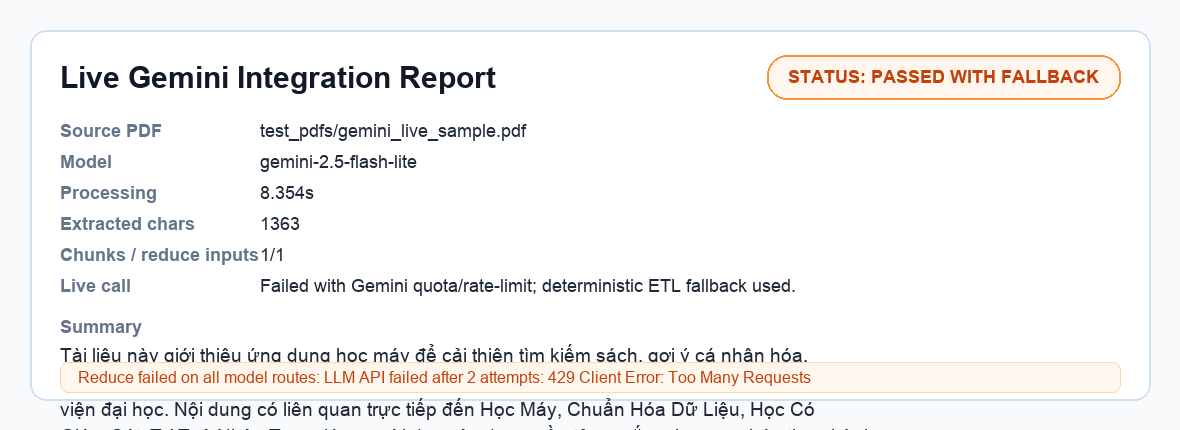
\includegraphics[width=0.9\textwidth]{figures/ch07/test-results/ai-gemini-live-result.png}
    }{
        \fbox{\parbox[c][5cm][c]{0.9\textwidth}{\centering Placeholder: kết quả live Gemini tại \texttt{figures/ch07/test-results/ai-gemini-live-result.png}}}
    }
    \caption{Artifact chạy live Gemini trên PDF mẫu}
    \label{fig:ai_gemini_live_result}
\end{figure}

Kịch bản live này kiểm tra trực tiếp khả năng gọi Gemini và sinh metadata từ PDF
mẫu. Khi khóa API còn quota, artifact thành công chứa
\texttt{master\_summary}, \texttt{tags}, \texttt{tags\_en}, \texttt{audience},
số chunk và thời gian xử lý. Nếu Gemini trả lỗi quota/rate-limit, script ghi rõ
trạng thái live thất bại, redact API key, rồi có thể chạy nhánh fallback xác
định của AI ETL để vẫn nghiệm thu được phần đọc PDF, chia chunk và định dạng
metadata đầu ra.

\subsection{Đánh giá và giới hạn}

Phần kiểm thử frontend đã bao phủ các logic dùng chung và các hợp đồng
giao tiếp có giá trị cao: localize lỗi backend, notification đa ngôn ngữ, theme
toàn cục, language toàn cục, xác thực, upload, contact map, helper đặt trước và
service layer cho search/AI/PayOS/wishlist/rating. Các test này giúp nhóm tự
tin hơn khi sửa UI hoặc đổi message từ backend, vì những lỗi sai ngôn ngữ, sai
role, sai endpoint hoặc sai payload sẽ được phát hiện trước khi demo.

Tuy nhiên, nhóm vẫn phân biệt rõ giữa test frontend trong môi trường
\texttt{jsdom} và kiểm thử E2E trên trình duyệt thật. Bộ test này đủ cho
tầng unit/context/component/service contract, nhưng các luồng end-to-end như
đăng nhập thật, tìm kiếm sách, đặt trước, nhận sách, thanh toán PayOS và nhận
WebSocket notification vẫn nên được kiểm thử bằng Playwright hoặc kịch bản demo
tích hợp sau khi backend/AI service cùng chạy.

\section{Kiểm thử Backend}

Backend được kiểm thử bằng JUnit 5, Mockito, MockMvc, Spring Boot Test và
Testcontainers. Nhóm tách kiểm thử backend thành hai tầng: tầng unit/controller
chạy nhanh với mock để kiểm tra nhánh nghiệp vụ và hợp đồng API; tầng
integration chạy với PostgreSQL thật trong Docker để xác minh migration, dữ
liệu seed và các truy vấn native SQL quan trọng.

\subsection{Môi trường và cấu hình kiểm thử Backend}

Các module backend dùng Maven Surefire để chạy test. Với test tích hợp trong
\texttt{library-bootstrap}, nhóm dùng Testcontainers để khởi động
\texttt{postgres:15-alpine}, sau đó để Flyway chạy toàn bộ migration từ
\texttt{V1} đến \texttt{V22}. Cách này giúp kiểm thử trên schema thật của hệ
thống thay vì dùng database giả hoặc H2 không tương thích hoàn toàn với
PostgreSQL.

\begin{table}[H]
\centering
\small
\begin{tabularx}{\textwidth}{|p{4cm}|X|}
\hline
\textbf{Thành phần} & \textbf{Cấu hình sử dụng} \\
\hline
Test runner & JUnit 5, Maven Surefire, chạy bằng \texttt{mvn test}. \\
\hline
Mock unit test & Mockito và AssertJ cho use case/service. \\
\hline
Controller test & MockMvc standalone, kiểm request binding, validation và response JSON. \\
\hline
Integration test & Spring Boot Test với Testcontainers \texttt{1.21.4}. \\
\hline
Database test & Docker Engine \texttt{29.4.3}, container \texttt{postgres:15-alpine}. \\
\hline
Migration & Flyway chạy 29 migration trên database test, gồm migration dọn schema/index, metadata AI, admin/policy/audit và transaction notes cuối cùng. \\
\hline
Test profile & \texttt{application-test.yml}, tắt Kafka listener và scheduler để test không phụ thuộc dịch vụ ngoài. \\
\hline
\end{tabularx}
\caption{Cấu hình kiểm thử Backend}
\label{tab:be_test_env}
\end{table}


\begin{figure}[H]
    \centering
    \IfFileExists{figures/ch07/test-results/be-test-result.png}{
        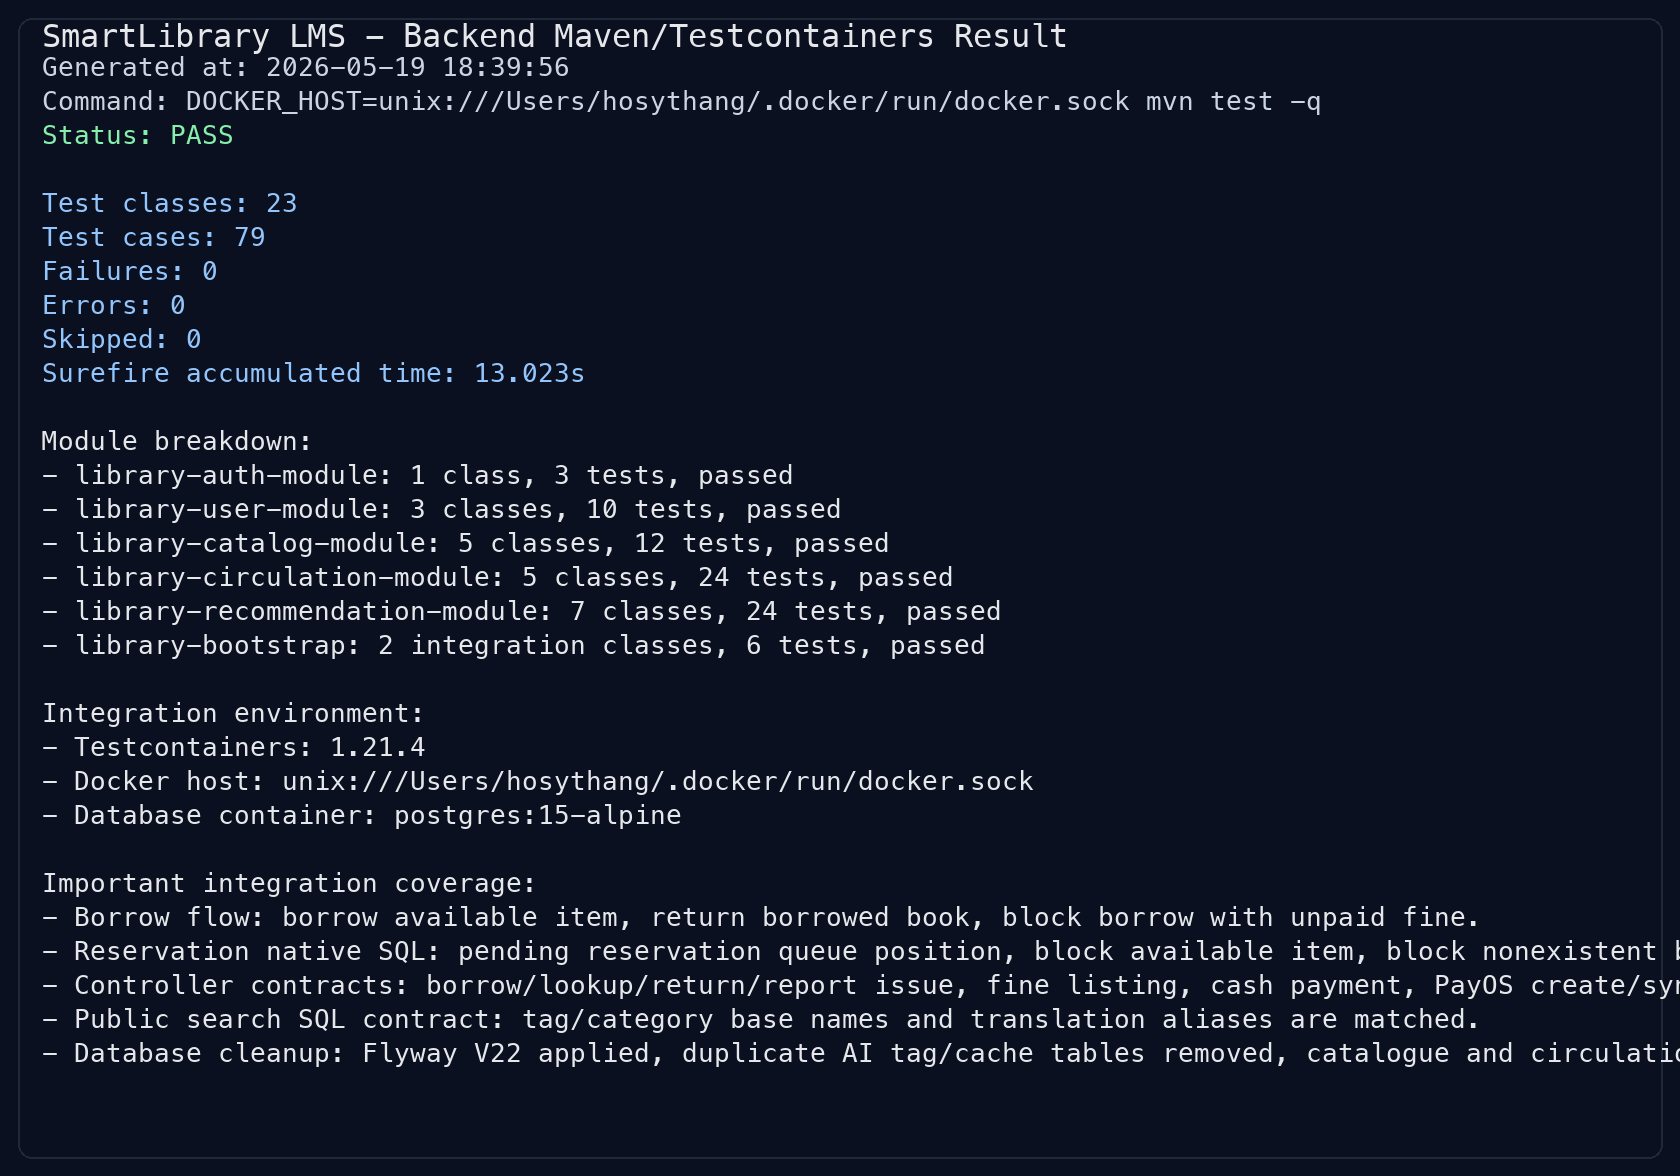
\includegraphics[width=0.9\textwidth]{figures/ch07/test-results/be-test-result.png}
    }{
        \fbox{\parbox[c][5cm][c]{0.9\textwidth}{\centering Placeholder: kết quả backend tại \texttt{figures/ch07/test-results/be-test-result.png}}}
    }
    \caption{Kết quả chạy bộ test Backend}
    \label{fig:be_test_result}
\end{figure}

\subsection{Phạm vi test Backend đã hiện thực}

Bộ test backend có 23 test class với 79 test case. Phạm vi được chọn
theo các luồng cốt lõi nhóm đã xây dựng: đăng ký/xác thực, notification, catalog
tài liệu, mượn--trả sách, đặt trước, rating/wishlist, AI gateway và callback từ
AI service. Với admin console và quy định mượn trả cấu hình từ DB, các test
circulation sử dụng mock \texttt{CirculationPolicyService}, bảo đảm unit test
phản ánh đúng cách runtime đọc policy thay vì giả định hằng số cứng.

\begin{table}[H]
\centering
\small
\begin{tabularx}{\textwidth}{|p{4.2cm}|p{2.2cm}|p{2cm}|X|}
\hline
\textbf{Module} & \textbf{Số class} & \textbf{Số test} & \textbf{Nội dung chính} \\
\hline
\texttt{library-auth-module} & 1 & 3 & Controller đăng ký, payload hợp lệ và validation email/student id. \\
\hline
\texttt{library-user-module} & 3 & 10 & Signup use case, notification page, unread count, mark read và mark all read. \\
\hline
\texttt{library-catalog-module} & 5 & 12 & Tạo publication/item, document upload URL, save document URL, public search SQL contract và publication controller. \\
\hline
\texttt{library-circulation-module} & 5 & 24 & Borrow request, return book, overdue fine, unpaid fine, borrow/reservation limit lấy từ \texttt{CirculationPolicyService}, reservation use case, transaction controller và fine/PayOS controller. \\
\hline
\texttt{library-recommendation-module} & 7 & 24 & Wishlist, rating, AI gateway fallback, semantic/recommendation contract và signed AI callback. \\
\hline
\texttt{library-bootstrap} & 2 & 6 & Integration với PostgreSQL thật: borrow/return flow và reservation native SQL. \\
\hline
\textbf{Tổng cộng} & \textbf{23} & \textbf{79} & \textbf{Toàn bộ pass}. \\
\hline
\end{tabularx}
\caption{Tổng hợp test Backend theo module}
\label{tab:be_test_modules}
\end{table}

\subsection{Kết quả thực thi Backend}

Bộ test backend cuối cùng chạy thành công toàn bộ. Kết quả chi tiết được lưu tại
thư mục \texttt{figures/test-results}, gồm file tóm tắt
\texttt{be-test-result.txt} và log Maven đầy đủ
\texttt{be-full-test-result.txt}.

\begin{table}[H]
\centering
\small
\begin{tabularx}{\textwidth}{|p{4cm}|X|}
\hline
\textbf{Chỉ số} & \textbf{Kết quả} \\
\hline
Test classes & \textbf{23}. \\
\hline
Test cases & \textbf{79 passed / 79 total}. \\
\hline
Failures & \textbf{0}. \\
\hline
Errors & \textbf{0}. \\
\hline
Skipped & \textbf{0}. \\
\hline
Thời gian Surefire & Khoảng \textbf{13.023s}. \\
\hline
Kết luận & Bộ test backend pass toàn bộ ở tầng unit/controller và integration PostgreSQL. \\
\hline
\end{tabularx}
\caption{Kết quả kiểm thử Backend}
\label{tab:be_test_result}
\end{table}

\subsection{Đánh giá và giới hạn}

Bộ test backend đã bao phủ các thành quả chính của hệ thống: quản lý
ấn phẩm, upload tài liệu, tìm kiếm public, đăng ký người dùng, notification,
mượn--trả sách, đặt trước, phí phạt/thanh toán, rating, wishlist và tích hợp AI. Đặc biệt, nhóm đã
kiểm thử integration với PostgreSQL thật bằng Testcontainers để chứng minh các
native SQL và migration hoạt động trên môi trường gần với triển khai thực tế.

Giới hạn còn lại là bộ test chưa thay thế hoàn toàn kiểm thử E2E nhiều dịch vụ
cùng lúc với frontend, backend, AI service, Kafka và PayOS sandbox đều đang
chạy. Tuy nhiên, ở phạm vi backend độc lập, bộ test đủ để chứng minh
các use case cốt lõi, controller contract và truy vấn database quan trọng hoạt
động đúng.

\section{Kiểm thử AI Service}

AI service là phần chịu trách nhiệm xử lý tài liệu PDF, tạo vector embedding,
sinh metadata học thuật, tìm kiếm ngữ nghĩa và gợi ý sách. Vì vậy nhóm không chỉ
kiểm thử API trả đúng schema, mà còn kiểm thử các ràng buộc chất lượng ở bên
trong pipeline: làm sạch PDF, chia chunk ổn định, reduce không dùng metadata
catalog để viết summary, tag tiếng Việt đúng 5 nhãn, alias tiếng Anh khớp
1--1, SQL ghi vào đúng schema \texttt{public}/\texttt{ai\_engine}, hybrid search
ưu tiên lexical trước semantic với truy vấn ngắn, recommender có fallback và
worker callback có chữ ký HMAC.

Riêng đối với phân hệ schema AI, kiểm thử giao ước dữ liệu (test contract) tập trung xác nhận pipeline thực hiện ghi nhận chính xác vào các đích lưu trữ sau:
\begin{itemize}
    \item \textbf{Dữ liệu Vector:} Ghi cấu trúc vector vào bảng \texttt{ai\_engine.publication\_vectors}.
    \item \textbf{Phân loại dữ liệu (Tags):} Định tuyến dữ liệu tag vào phân hệ chung thông qua \texttt{public.tags} và \texttt{public.publication\_tags}.
    \item \textbf{Bản địa hóa ngôn ngữ:} Lưu trữ cấu hình alias tại \texttt{public.tag\_translations}.
\end{itemize}
Đồng thời, phạm vi kiểm thử đảm bảo hệ thống hoàn toàn cô lập, không phát sinh phụ thuộc vào các bảng nằm ngoài cấu trúc schema đích bao gồm: \texttt{ai\_engine.tags}, \texttt{ai\_engine.publication\_tags} và \texttt{ai\_engine.recommendation\_cache}.

\subsection{Môi trường kiểm thử AI}

Bộ test AI được viết bằng \texttt{pytest}. Các test chính chạy offline, không gọi
Gemini thật, không cần PostgreSQL, RabbitMQ hoặc backend đang chạy. Những test
tích hợp live cho API vẫn được giữ trong thư mục \texttt{tests/integration} và
chỉ chạy khi bật biến môi trường \texttt{RUN\_LIVE\_AI\_CONTRACT\_TESTS=1}.
Cách tách này giúp nhóm có một bộ regression nhanh để chạy thường xuyên, đồng
thời vẫn có đường kiểm thử end-to-end khi cần đo latency với service thật.

\begin{table}[H]
\centering
\small
\begin{tabularx}{\textwidth}{|p{4cm}|X|}
\hline
\textbf{Thành phần} & \textbf{Cấu hình sử dụng} \\
\hline
Test runner & \texttt{pytest 8.3.5}, chạy bằng \texttt{PYTHONPATH=. ./venv/bin/python -m pytest -q}. \\
\hline
Mock LLM & Stub \texttt{GeminiClient.\_call} để trả JSON cố định, không gọi API ngoài. \\
\hline
Mock database & Fake connection/cursor để bắt SQL và tham số, không cần PostgreSQL thật. \\
\hline
Mock gateway & Monkeypatch các hàm search/recommendation để kiểm thứ tự merge, limit và fallback. \\
\hline
Mock worker & Mock Celery signal/app và HTTP request để kiểm payload, download và HMAC callback. \\
\hline
Live integration & 3 test contract/latency được skip mặc định, chỉ bật khi có AI API thật qua \texttt{AI\_API\_BASE\_URL}. \\
\hline
\end{tabularx}
\caption{Cấu hình kiểm thử AI Service}
\label{tab:ai_test_env}
\end{table}


\begin{figure}[H]
    \centering
    \IfFileExists{figures/ch07/test-results/ai-pytest-result.png}{
        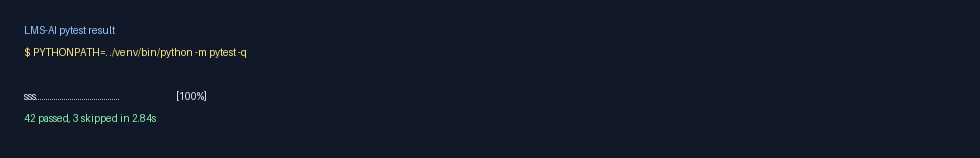
\includegraphics[width=0.9\textwidth]{figures/ch07/test-results/ai-pytest-result.png}
    }{
        \fbox{\parbox[c][5cm][c]{0.9\textwidth}{\centering Placeholder: kết quả AI pytest tại \texttt{figures/ch07/test-results/ai-pytest-result.png}}}
    }
    \caption{Kết quả chạy bộ test AI Service}
    \label{fig:ai_pytest_result}
\end{figure}

\subsection{Phạm vi test AI đã hiện thực}

Bộ test AI có 9 file test với 47 test case được collect. Trong đó 44
test offline pass và 3 test live integration được skip mặc định. Các test được
chia theo module thay vì chỉ theo endpoint, vì lỗi trong AI thường xuất hiện ở
giữa pipeline: PDF nhiễu làm chunk sai, LLM trả JSON lệch, tag bị generic, SQL
ghi sai schema hoặc hybrid search merge sai thứ tự.

\begin{table}[H]
\centering
\small % Nâng cỡ chữ lên để đọc rõ ràng, tương thích chuẩn báo cáo
\renewcommand{\arraystretch}{1.5} % Tạo không gian thở rộng rãi cho từng dòng
\begin{tabularx}{\textwidth}{|p{5.6cm}|>{\raggedright\arraybackslash}X|p{1.8cm}|}
\hline
\textbf{File test} & \textbf{Nội dung kiểm thử} & \textbf{Số test} \\
\hline
\texttt{tests/test\_ai\_metadata\_} \newline \texttt{quality.py} & Fallback tag, summary chỉ dựa trên PDF content, lọc tag generic/title/category và alias tiếng Anh. & 5 \\
\hline
\texttt{tests/test\_pdf\_processing.py} & Làm sạch header/footer/số trang, bỏ ký tự null, ghép từ bị xuống dòng, chunk id ổn định và validate \texttt{chunk\_overlap}. & 4 \\
\hline
\texttt{tests/test\_llm\_client.py} & Parse JSON từ Gemini, lỗi response rỗng, reduce metadata, lọc tag xấu, giữ alias \texttt{tags\_en} đúng cặp và reject summary kiểu catalog. & 6 \\
\hline
\texttt{tests/test\_pipeline\_core.py} & Chọn representative chunks, áp budget reduce, fallback khi LLM lỗi, optional English metadata translation và hash file/URL. & 7 \\
\hline
\texttt{tests/test\_database\_sql\_} \newline \texttt{contract.py} & SQL contract cho vector, publication tags, \texttt{public.tags}, \texttt{public.tag\_translations} và điều kiện đủ AI output. & 5 \\
\hline
\texttt{tests/test\_api\_service\_} \newline \texttt{contract.py} & pgvector literal, tokenize tiếng Việt không dấu, merge hybrid search, giới hạn \texttt{limit}, lexical-first cho query ngắn và fallback recommendation khi ALS lỗi. & 9 \\
\hline
\texttt{tests/test\_recommender\_} \newline \texttt{engine.py} & ALS bundle settings, trọng số interaction, cold user và danh sách publication id từ model recommendation. & 4 \\
\hline
\texttt{tests/test\_worker\_contract.py} & Validate payload RabbitMQ, download PDF tạm, webhook JSON compact và chữ ký HMAC \texttt{timestamp.body}. & 4 \\
\hline
\texttt{tests/integration/test\_api\_} \newline \texttt{contract\_and\_latency.py} & Health, semantic search và recommendation contract/latency với AI API thật; skip mặc định. & 3 skip \\
\hline
\textbf{Tổng cộng} & \textbf{44 pass, 3 skip} & \textbf{47} \\
\hline
\end{tabularx}
\caption{Các file test AI Service đã hiện thực}
\label{tab:ai_test_files}
\end{table}
\subsection{Kết quả thực thi AI}

Bộ test AI cuối cùng chạy thành công toàn bộ phần offline. Ba test integration
live được collect nhưng skip mặc định vì chúng yêu cầu AI API thật đang chạy và
có dữ liệu/embedding trong database.

\begin{table}[H]
\centering
\small
\begin{tabularx}{\textwidth}{|p{4cm}|X|}
\hline
\textbf{Chỉ số} & \textbf{Kết quả} \\
\hline
Test files & \textbf{9}. \\
\hline
Test cases collected & \textbf{47}. \\
\hline
Passed & \textbf{44}. \\
\hline
Skipped & \textbf{3} live integration tests. \\
\hline
Failures/Errors & \textbf{0}. \\
\hline
Thời gian chạy & Khoảng \textbf{3.94s} trên môi trường local. \\
\hline
Kết luận & Bộ test AI pass toàn bộ ở tầng unit/contract offline; test live được giữ để chạy khi có môi trường tích hợp. \\
\hline
\end{tabularx}
\caption{Kết quả kiểm thử AI Service}
\label{tab:ai_test_result}
\end{table}

\subsection{Benchmark định lượng chất lượng AI}

Để tránh đánh giá AI bằng nhận xét cảm tính, nhóm bổ sung benchmark định lượng
trên bộ dữ liệu thật \texttt{evaluation/ai\_quality\_cases.real.json}. Bộ này
gồm 6 đầu sách đã được force reprocess bằng pipeline AI hiện tại và 4 truy vấn
tìm kiếm ngữ nghĩa có ground truth thủ công. Script
\texttt{scripts/ai\_quality\_benchmark.py} đọc metadata mới nhất từ PostgreSQL,
gọi live endpoint \texttt{/api/v1/semantic-search}, sau đó tính các metric phù
hợp với từng bài toán: \texttt{Precision/Recall/F1} cho tag,
\texttt{Keyword coverage} và \texttt{Hallucination guard} cho summary,
\texttt{MRR}, \texttt{Recall@5} và \texttt{nDCG@5} cho ranking, đồng thời đo
\texttt{p50}/\texttt{p95} latency.

\begin{figure}[H]
    \centering
    \IfFileExists{figures/ch07/test-results/ai-quality-benchmark-result.png}{
        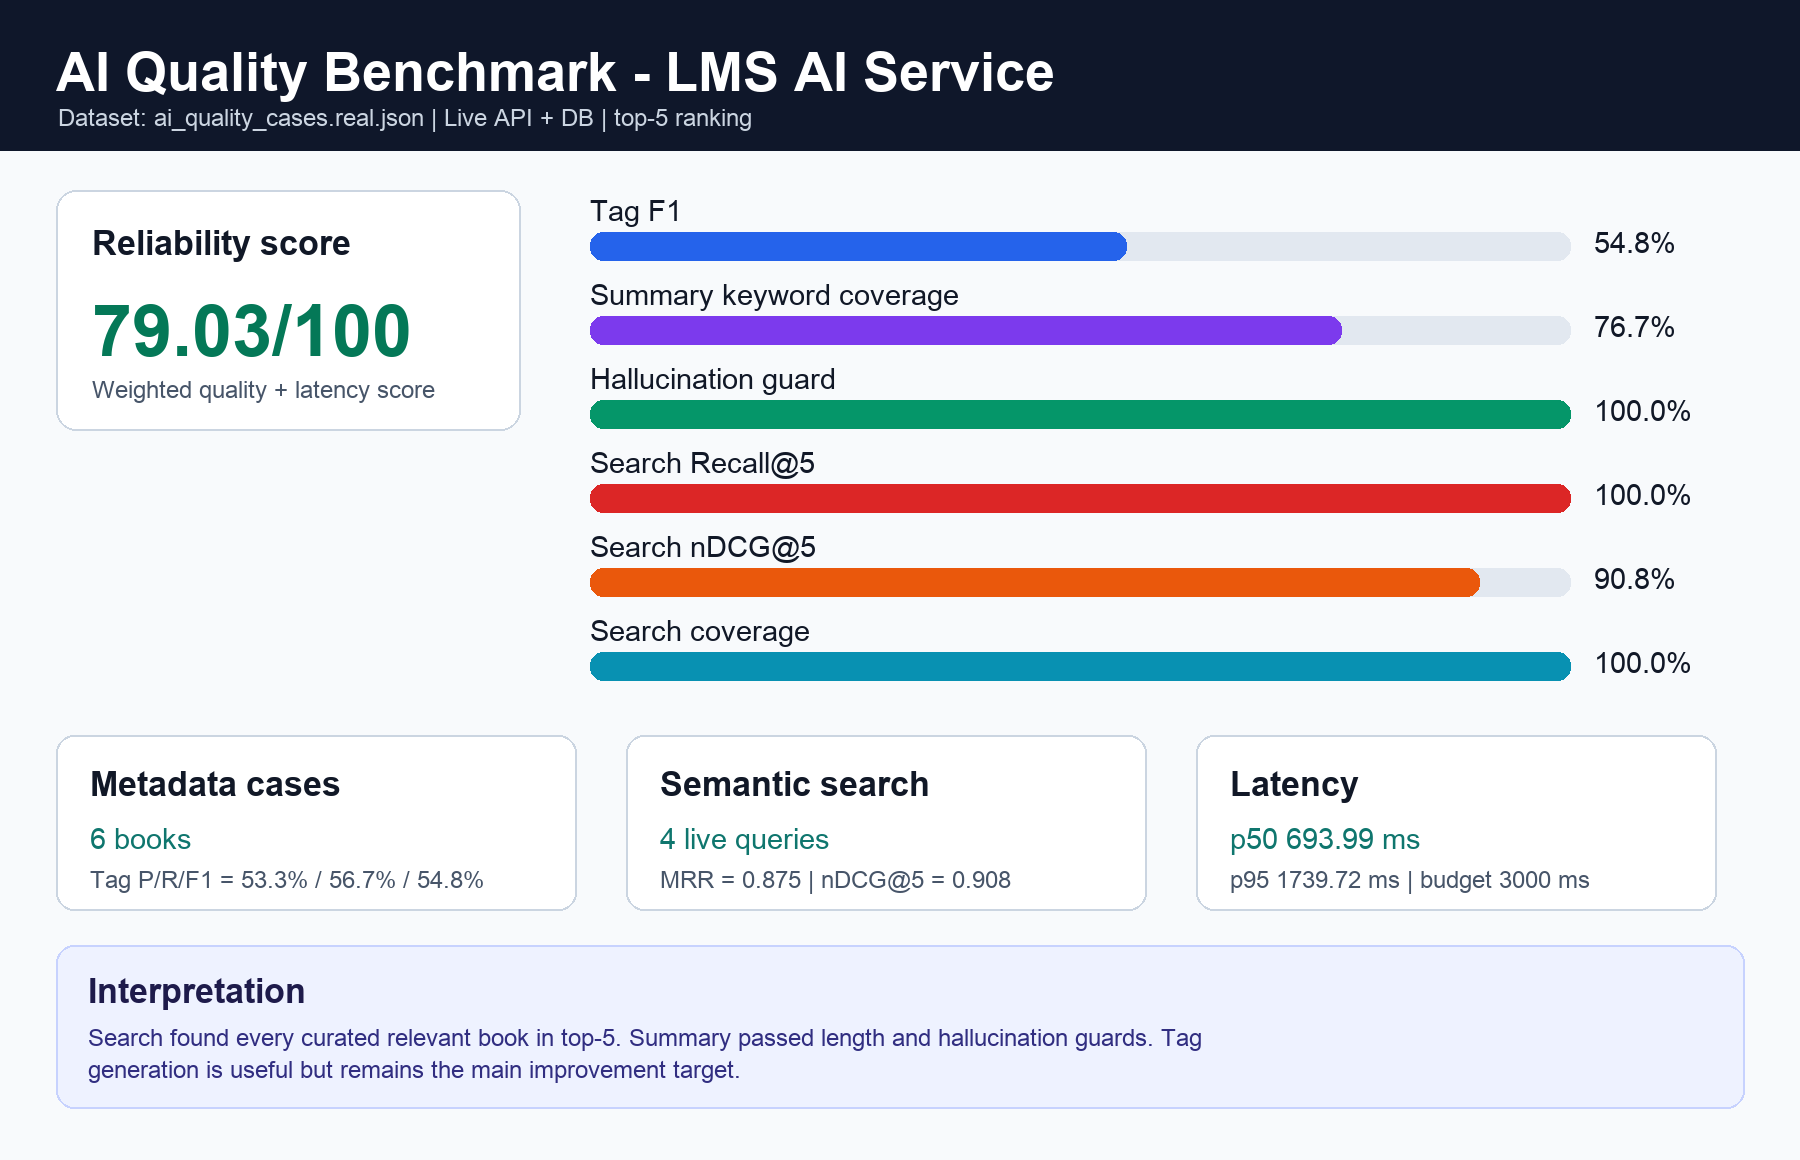
\includegraphics[width=0.95\textwidth]{figures/ch07/test-results/ai-quality-benchmark-result.png}
    }{
        \fbox{\parbox[c][5cm][c]{0.9\textwidth}{\centering Placeholder: kết quả benchmark AI tại \texttt{figures/ch07/test-results/ai-quality-benchmark-result.png}}}
    }
    \caption{Kết quả benchmark định lượng chất lượng AI trên dữ liệu thật}
    \label{fig:ai_quality_benchmark_result}
\end{figure}

\begin{table}[H]
\centering
\small
\begin{tabularx}{\textwidth}{|p{4.5cm}|X|p{2.5cm}|}
\hline
\textbf{Nhóm đánh giá} & \textbf{Metric} & \textbf{Kết quả} \\
\hline
Tổng hợp & Reliability score có trọng số từ metadata, search và latency & \textbf{79.03/100} \\
\hline
Metadata & Tag precision / recall / F1 so với tag chuẩn thủ công & \textbf{53.3\% / 56.7\% / 54.8\%} \\
\hline
Summary & Keyword coverage, length OK và hallucination guard & \textbf{76.7\%, 100.0\%, 100.0\%} \\
\hline
Semantic search & Recall@5, MRR và nDCG@5 trên 4 truy vấn live & \textbf{100.0\%, 0.875, 0.908} \\
\hline
Coverage & Tỉ lệ query trả về danh sách kết quả khác rỗng & \textbf{100.0\%} \\
\hline
Runtime & p50 / p95 latency khi gọi live AI API, budget 3000ms & \textbf{693.99ms / 1739.72ms} \\
\hline
\end{tabularx}
\caption{Kết quả benchmark AI trên bộ ground truth thật}
\label{tab:ai_quality_benchmark_result}
\end{table}

Kết quả này cho thấy phần search là điểm mạnh rõ nhất: toàn bộ truy vấn đều tìm
được sách đúng trong top 5, với \texttt{nDCG@5 = 0.908} và \texttt{MRR = 0.875},
tức là kết quả đúng thường xuất hiện rất sớm trong danh sách. Summary cũng đạt
ngưỡng an toàn tốt: độ phủ keyword đạt \textbf{76.7\%}, tất cả summary nằm trong
giới hạn độ dài và không chứa forbidden terms trong bộ kiểm thử.

Điểm cần cải thiện nằm ở sinh tag. \texttt{Tag F1 = 54.8\%} chưa đạt ngưỡng
mong muốn cho báo cáo dài hạn, nhưng đây là số liệu thật và có thể giải thích
được: một số tag đúng hướng nhưng khác cách đặt nhãn so với ground truth, và có
trường hợp sinh một tag lệch domain. Nhóm vẫn đưa chỉ số này vào báo cáo thay vì
ẩn đi, vì mục tiêu kiểm thử AI là chứng minh hệ thống được đo lường và kiểm soát
bằng số liệu lặp lại được, không phải chỉ trình bày các ví dụ đẹp.

Phần recommendation chưa được chấm trong benchmark này vì chưa có bộ user
profile ground truth được curator gán thủ công. Nếu tự gán bừa nhãn recommend để
làm đẹp điểm thì kết quả không có giá trị kiểm thử. Do đó báo cáo hiện tại chỉ
kết luận định lượng cho metadata, summary, semantic search và latency; còn
recommendation được kiểm bằng unit/contract test và cần bổ sung bộ ground truth
riêng khi có đủ dữ liệu hành vi người dùng thật.

\subsection{Đánh giá và giới hạn}

Bộ test AI đã bao phủ các tính năng chính của service: xử lý PDF,
chunking, metadata reduce, tag quality, fallback khi LLM lỗi, alias tiếng Anh,
ghi SQL đúng schema, semantic search hybrid, recommendation CBF/ALS/trending và
worker callback bảo mật. Quan trọng hơn, các test đã bắt được lỗi thật trong
pipeline PDF và align \texttt{tags\_en}, qua đó giúp chất lượng AI output ổn
định hơn trước khi demo.

Giới hạn còn lại là các test offline chưa đo chất lượng ngôn ngữ thực tế của
Gemini và chưa đo latency thật trên tập dữ liệu lớn. Vì vậy nhóm vẫn giữ 3 test
integration live để chạy khi PostgreSQL, model embedding và AI API đang hoạt
động; các test này phù hợp cho giai đoạn nghiệm thu tích hợp hoặc benchmark
riêng, còn bộ 44 test offline phù hợp để chạy thường xuyên sau mỗi lần sửa code.

\section{Kiểm thử theo yêu cầu phi chức năng}

Bên cạnh kiểm thử chức năng theo từng phân hệ, nhóm đối chiếu lại các yêu cầu
phi chức năng đã nêu ở Mục~\ref{subsec:YeuCauPhiChucNang}. Không phải mọi yêu
cầu phi chức năng đều đo được hoàn toàn bằng unit test; ví dụ tính dễ học của
giao diện vẫn cần đánh giá thủ công trong quá trình demo. Tuy nhiên, các yêu
cầu có tiêu chí kỹ thuật rõ ràng như giới hạn truy vấn, timeout, fallback,
phân quyền, chữ ký callback và cấu trúc module đều có thể được kiểm chứng bằng
test tự động hoặc test contract.

\begin{table}[H]
\centering
\scriptsize
\begin{tabularx}{\textwidth}{|p{3.1cm}|p{4.4cm}|X|p{2.1cm}|}
\hline
\textbf{Yêu cầu phi chức năng} & \textbf{Tiêu chí kiểm chứng được} & \textbf{Test/nhóm test liên quan} & \textbf{Kết quả} \\
\hline
Tính khả dụng & Các state toàn cục và helper UI phải nhất quán: ngôn ngữ, theme, thông báo, trạng thái đặt trước, lỗi nghiệp vụ và upload. & \texttt{LanguageContext}, \texttt{ThemeContext}, notification localization, \texttt{reservationUtils}, component dùng chung và service contract frontend. & 58/58 frontend pass. \\
\hline
Hiệu năng & Request có phân trang/giới hạn kết quả; truy vấn AI và recommendation không được nhận limit không kiểm soát; SQL dài có statement timeout. & Public search backend cap page size tối đa 50; AI semantic search cap \texttt{limit} theo cấu hình; recommender dùng \texttt{SET LOCAL statement\_timeout}; live latency test giữ để benchmark khi có môi trường thật. & Pass; live latency skip mặc định. \\
\hline
Độ tin cậy & Dịch vụ phụ trợ lỗi không được làm sập nghiệp vụ chính; AI/Gemini lỗi phải có fallback xác định. & AI gateway backend trả fallback khi HTTP 500; AI ETL fallback metadata khi LLM lỗi; recommendation fallback sang content-based/trending khi ALS lỗi; worker callback ghi trạng thái rõ ràng. & Pass. \\
\hline
Bảo mật & API nhạy cảm phải dựa trên JWT/role; callback/webhook phải xác thực chữ ký; upload PDF không đi qua endpoint mở tùy ý. & Auth/controller test, admin endpoint contract, PayOS webhook reject chữ ký sai, AI callback HMAC reject thiếu/sai chữ ký, frontend upload dùng presigned URL và raw axios. & Pass. \\
\hline
Khả năng bảo trì và mở rộng & Code tách theo frontend, backend module và AI service; hợp đồng giữa các service ổn định để thay đổi nội bộ không làm vỡ tích hợp. & 11 frontend suite, 23 backend test class và 9 AI test file tách theo module; service contract kiểm URL/payload; SQL contract kiểm schema \texttt{public}/\texttt{ai\_engine}. & Pass. \\
\hline
\end{tabularx}
\caption{Đối chiếu kiểm thử với yêu cầu phi chức năng}
\label{tab:nfr_test_mapping}
\end{table}

Từ bảng~\ref{tab:nfr_test_mapping}, các yêu cầu phi chức năng có khả năng
kiểm chứng bằng mã nguồn đều đã được đưa vào bộ test regression. Phần hiệu năng
ở mức unit/contract tập trung vào các ràng buộc chống quá tải như pagination,
limit và timeout; phần đo latency thật được tách thành nhóm integration live để
chỉ chạy khi có đủ backend, database, model embedding và dữ liệu mẫu. Cách tách
này giúp bộ test thường xuyên vẫn chạy nhanh, đồng thời vẫn giữ được kịch bản
nghiệm thu phi chức năng khi triển khai trong môi trường tích hợp. Các kết quả
chạy test đã được lưu thành artifact ảnh tại
\texttt{figures/ch07/test-results/} và được nhúng trực tiếp trong các mục kiểm
thử frontend, backend và AI ở phía trên, nhờ đó phần đối chiếu phi chức năng
không chỉ dừng ở mô tả mà có bằng chứng thực nghiệm đi kèm.

\chapter{Triển khai hệ thống}

\section{Caddy --- Reverse Proxy}

\subsection{Vai trò của Caddy}

Caddy đóng vai trò là reverse proxy trung tâm, tiếp nhận toàn bộ traffic public
từ bên ngoài trên cổng 80/443, tự động cấp HTTPS và định tuyến request đến đúng
dịch vụ nội bộ. Kiến trúc này mang lại hai lợi ích chính: thứ nhất, các cổng
nội bộ của từng container không bị lộ trực tiếp ra internet; thứ hai, client chỉ
cần giao tiếp với một địa chỉ duy nhất là \texttt{https://library74.uk}. Trong
mô hình hiện tại, Nginx vẫn được sử dụng bên trong container frontend để phục vụ
static build của React/Vite, còn Caddy là lớp entrypoint và reverse proxy ở bên
ngoài.

\section{Môi trường sản xuất}

\subsection{Docker Compose sản xuất}

Trong repository hiện tại, cấu hình container được tách theo từng thành phần:
\texttt{LMS\_BE/docker-compose.yml} quản lý PostgreSQL và Kafka cho backend,
còn \texttt{LMS-AI/docker-compose.yml} quản lý RabbitMQ, FastAPI API server và
Celery worker. Frontend và backend có Dockerfile riêng để build image triển
khai. Khi đưa lên server, các thành phần này cần được đặt trong cùng một mạng
triển khai hoặc được cấu hình endpoint rõ ràng thông qua biến môi trường.

Luồng kết nối quan trọng nhất là backend gọi AI qua
\texttt{AI\_GATEWAY\_BASE\_URL}, còn AI service gọi ngược backend qua
\texttt{BACKEND\_WEBHOOK\_URL}. Secret ký callback của hai phía phải khớp nhau:
\texttt{AI\_CALLBACK\_SECRET} ở backend và \texttt{BACKEND\_WEBHOOK\_SECRET}
ở AI service.

Một điểm khác biệt quan trọng so với cấu hình phát triển là giá trị
\texttt{KAFKA\_CFG\_ADVERTISED\_LISTENERS} được thay đổi từ
\texttt{PLAINTEXT://localhost:9092} thành \texttt{PLAINTEXT://kafka:9092}.
Trong môi trường phát triển, Spring Boot chạy trên máy host nên dùng
\texttt{localhost}; trong môi trường container, Spring Boot nằm trong một
container khác và phải kết nối đến Kafka qua tên service Docker.

\begin{verbatim}
# Hạ tầng Backend
cd LMS_BE && docker compose up -d

# AI Service
cd ../LMS-AI && docker compose up -d --build

# Build image Backend và Frontend khi triển khai container hóa đầy đủ
cd ../LMS_BE && docker build -t lms-backend .
cd ../LMS_fe && docker build -t lms-frontend .
\end{verbatim}

\subsection{Quản lý biến môi trường và bảo mật}

Tất cả thông tin nhạy cảm của hệ thống được quản lý thông qua file \texttt{.env}
và không bao giờ được đưa vào mã nguồn (được liệt kê trong \texttt{.gitignore}).
Bảng~\ref{tab:env_vars} liệt kê các nhóm biến môi trường chính.

\begin{table}[h]
\centering
\small
\caption{Các nhóm biến môi trường của hệ thống}
\label{tab:env_vars}
\begin{tabularx}{\textwidth}{|p{2.8cm}|p{6.3cm}|X|}
\hline
\textbf{Nhóm} & \textbf{Biến} & \textbf{Mục đích} \\
\hline
Cơ sở dữ liệu
  & \texttt{DATABASE\_URL} \newline
    \texttt{DATABASE\_USERNAME} \newline
    \texttt{DATABASE\_PASSWORD}
  & Kết nối PostgreSQL \\
\hline
JWT
  & \texttt{EXP\_TOKEN} \newline
    \texttt{EXP\_REFRESH\_TOKEN}
  & Thời hạn Access/Refresh token \\
\hline
OAuth2 Google
  & \texttt{GOOGLE\_CLIENT\_ID} \newline
    \texttt{GOOGLE\_CLIENT\_SECRET} \newline
    \texttt{OAUTH2\_REDIRECT\_URI}
  & Đăng nhập Google \\
\hline
Email
  & \texttt{MAIL\_SENDER\_USERNAME} \newline
    \texttt{MAIL\_SENDER\_PASSWORD}
  & Gửi email qua SMTP \\
\hline
AWS S3
  & \texttt{AWS\_ACCESS\_KEY} \newline
    \texttt{AWS\_SECRET\_KEY}
  & Lưu trữ file (ảnh bìa, tài liệu) \\
\hline
AI Gateway
  & \texttt{AI\_GATEWAY\_BASE\_URL} \newline
    \texttt{AI\_CALLBACK\_SECRET} \newline
    \texttt{AI\_CALLBACK\_MAX\_CLOCK\_} \newline
    \texttt{SKEW\_SECONDS}
  & Backend gọi AI service và xác thực callback \\
\hline
AI Service
  & \texttt{GEMINI\_API\_KEY} \newline
    \texttt{RABBITMQ\_URL} \newline
    \texttt{BACKEND\_WEBHOOK\_URL} \newline
    \texttt{BACKEND\_WEBHOOK\_SECRET}
  & Chạy FastAPI, Celery, Gemini và webhook \\
\hline
PayOS
  & \texttt{CLIENT\_ID\_PAYOS} \newline
    \texttt{API\_KEY\_PAYOS} \newline
    \texttt{CHECKSUM\_KEY\_PAYOS}
  & Tạo và xác thực thanh toán phí phạt \\
\hline
Frontend
  & \texttt{VITE\_API\_BASE\_URL} \newline
    \texttt{VITE\_API\_TIMEOUT}
  & Cấu hình endpoint API và timeout khi build Vite \\
\hline
\end{tabularx}
\end{table}

Khi triển khai lên máy chủ, mỗi thành phần có file môi trường riêng:
\texttt{LMS\_BE/.env}, \texttt{LMS-AI/.env} và cấu hình build cho
\texttt{LMS\_fe}. Các file này được tạo từ \texttt{.env.example}, điền giá trị
thực tế trên server và không đưa vào lịch sử git. Với Docker Compose, các biến
được tham chiếu qua \texttt{env\_file} hoặc truyền vào build argument để tránh
nhúng secret vào Docker image.

\subsection{Flyway Migration tự động}

Hệ thống sử dụng Flyway để quản lý phiên bản schema cơ sở dữ liệu. Khi
container Spring Boot khởi động, Flyway tự động thực thi các file migration
chưa được áp dụng theo thứ tự phiên bản trước khi ứng dụng nhận request.
Điều này đảm bảo schema cơ sở dữ liệu luôn đồng bộ với phiên bản ứng dụng
mà không cần can thiệp thủ công.

\begin{verbatim}
library-bootstrap/src/main/resources/db/migration/
+-- V1__create_schema.sql
+-- V8__ai_publication_etl_status.sql
+-- V14__metadata_translations.sql
+-- V20__schema_cleanup_and_ai_indexes.sql
\-- V22__cleanup_ai_metadata_junk.sql
\end{verbatim}

\section{Quy trình triển khai}

Quy trình triển khai hệ thống lên một máy chủ Linux mới bao gồm các bước sau:

\begin{enumerate}
    \item \textbf{Chuẩn bị máy chủ:} Cài đặt Docker Engine và Docker Compose
          Plugin trên máy chủ Ubuntu.

    \begin{verbatim}
curl -fsSL https://get.docker.com | sh
    \end{verbatim}

    \item \textbf{Sao chép mã nguồn:} Clone repository về máy chủ.

    \begin{verbatim}
git clone <repository-url>
cd LMS
    \end{verbatim}

    \item \textbf{Cấu hình môi trường:} Tạo file \texttt{.env} từ template và
          điền các giá trị thực tế (database credentials, API keys, v.v.).

    \begin{verbatim}
cp LMS_BE/.env.example LMS_BE/.env
cp LMS-AI/.env.example LMS-AI/.env
cp LMS_fe/.env.example LMS_fe/.env
# Chỉnh sửa các file .env với giá trị thực tế
    \end{verbatim}

    \item \textbf{Khởi động hệ thống:} Build image và khởi động tất cả container.

    \begin{verbatim}
cd LMS_BE && docker compose up -d
cd ../LMS-AI && docker compose up -d --build
    \end{verbatim}

    \item \textbf{Kiểm tra trạng thái:} Xác nhận tất cả container đang chạy.

    \begin{verbatim}
cd LMS_BE && docker compose ps
cd ../LMS-AI && docker compose ps
docker logs lms_ai_api
docker logs lms_ai_worker
    \end{verbatim}
\end{enumerate}

Sau khi khởi động, Flyway tự động chạy các migration của backend. AI service
kiểm tra schema AI, kết nối RabbitMQ, tải model embedding khi cần và sẵn sàng
nhận request tại endpoint đã cấu hình.

\section{Hạ tầng mạng: Domain và HTTPS}

\subsection{Tên miền (Domain)}

Trong bản triển khai demo, hệ thống sử dụng tên miền \texttt{library74.uk} để
người dùng truy cập bằng một địa chỉ ổn định thay vì ghi nhớ IP hoặc cổng dịch
vụ. DNS của domain được quản lý qua Cloudflare và trỏ về Google Cloud VPS. Tại
VPS, Caddy nhận request HTTPS, tự động xử lý chứng chỉ TLS và định tuyến request
đến frontend, backend API hoặc WebSocket theo path tương ứng.

Luồng kết nối sau khi đi vào backend tiếp tục được phân tách theo trách nhiệm:
Spring Boot xử lý nghiệp vụ chính và kết nối PostgreSQL/Kafka; backend gọi AI
Service qua \texttt{AI\_GATEWAY\_BASE\_URL}; AI worker xử lý PDF bất đồng bộ qua
RabbitMQ và callback kết quả về backend bằng chữ ký HMAC. Các tích hợp ngoài
như S3-compatible storage, PayOS, Gmail SMTP, Google OAuth2 và Gemini API được
kết nối từ backend hoặc AI worker theo đúng vai trò của từng dịch vụ.

\begin{figure}[h]
    \centering
    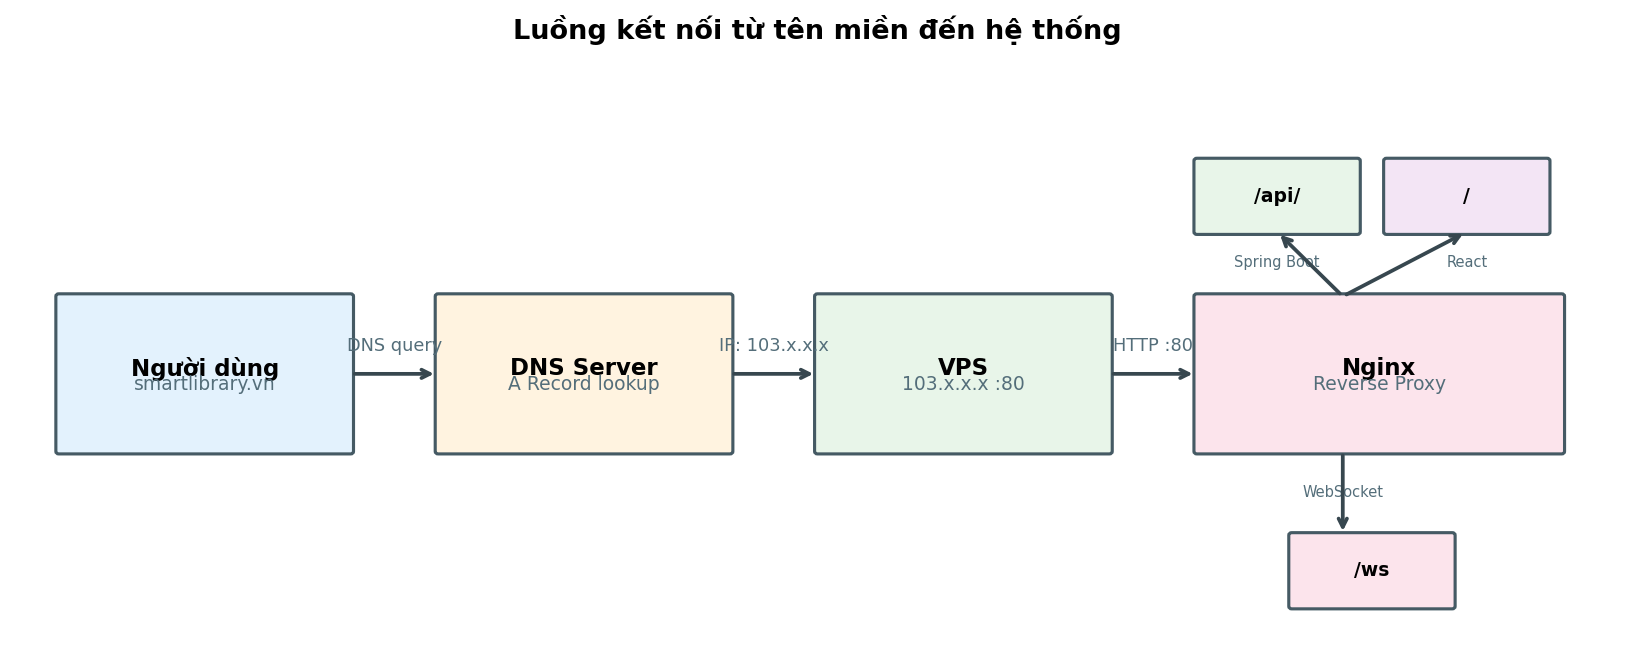
\includegraphics[width=0.95\textwidth]{figures/ch09/dns_flow.png}
    \caption{Luồng kết nối từ tên miền Library74 đến hệ thống production}
    \label{fig:dns_flow}
\end{figure}

\subsection{Tổng chi phí vận hành}

Bảng~\ref{tab:hosting_cost} được điều chỉnh theo chi phí triển khai hiện tại.
Tên miền \texttt{library74.uk} được mua theo năm, còn máy chủ demo đang chạy
trên Google Cloud Platform với cấu hình ước tính khoảng 92 USD/năm. Tại thời
điểm triển khai demo, GCP đang có ưu đãi miễn phí 3 tháng nên chi phí thực trả
ban đầu thấp hơn chi phí vận hành ổn định về sau.

\begin{table}[h]
\centering
\small
\caption{Chi phí vận hành hệ thống trong cấu hình demo}
\label{tab:hosting_cost}
\begin{tabularx}{\textwidth}{|p{3.5cm}|p{3.3cm}|p{2cm}|X|}
\hline
\textbf{Thành phần} & \textbf{Chi phí} & \textbf{Chu kỳ} & \textbf{Ghi chú} \\
\hline
Tên miền \texttt{library74.uk} & 5,3 USD & Năm & Khoản bắt buộc để giữ địa chỉ public của demo. \\
\hline
SSL/HTTPS & Miễn phí & 90 ngày hoặc tự động & Let's Encrypt hoặc chứng chỉ tự động từ reverse proxy/nhà cung cấp. \\
\hline
Google Cloud Platform & 92 USD & Năm & Chi phí theo cấu hình máy chủ demo; hiện đang được miễn phí 3 tháng đầu. \\
\hline
Lưu trữ file & Theo mức sử dụng & Tháng & Ảnh bìa/PDF dùng object storage hoặc cấu hình tương đương; chi phí phụ thuộc dung lượng thực tế. \\
\hline
API ngoài & Miễn phí trong phạm vi demo & Tháng & Google OAuth, Gmail SMTP, PayOS sandbox/quota demo và Gemini quota thử nghiệm. \\
\hline
\textbf{Tổng cố định ước tính} & \textbf{97,3 USD} & \textbf{Năm} & Chưa tính ưu đãi miễn phí 3 tháng GCP và chi phí phát sinh theo dung lượng/request thực tế. \\
\hline
\end{tabularx}
\end{table}

\noindent Như vậy, sau giai đoạn miễn phí ban đầu, chi phí cố định tối thiểu của
hệ thống chủ yếu gồm tên miền và máy chủ GCP, khoảng 97,3 USD/năm theo cấu hình
demo. Khi triển khai production thật, nhóm cần cập nhật lại theo dung lượng PDF,
số lượt truy vấn AI và chính sách giá của nhà cung cấp tại thời điểm vận hành.

% --- BẮT ĐẦU PHẦN TỔNG KẾT ---

\chapter{Tổng kết}

Dự án ``Hệ thống Quản lý Thư viện Trực tuyến tích hợp AI'' được xây dựng nhằm
số hóa các nghiệp vụ thư viện, đồng thời cải thiện trải nghiệm tra cứu và gợi ý
sách cho người dùng. Sau quá trình phân tích, thiết kế, hiện thực và kiểm thử,
nhóm đã hoàn thiện một hệ thống có đầy đủ ba lớp chính: Back-end nghiệp vụ,
Front-end người dùng và AI Service độc lập.

\section{Kết quả đạt được}

\subsection{Back-end nghiệp vụ}

Back-end được xây dựng bằng Spring Boot theo hướng \textbf{Modular Monolith},
tách thành các module có ranh giới rõ ràng:

\begin{itemize}
    \item \textbf{Auth/User:} Đăng ký, đăng nhập, JWT, refresh token, xác thực email,
    OAuth2, hồ sơ người dùng, phân quyền theo vai trò.
    \item \textbf{Catalog:} Quản lý ấn phẩm, tác giả, thể loại, nhà xuất bản, bản sao
    sách, upload tài liệu và metadata phục vụ AI.
    \item \textbf{Circulation:} Mượn/trả sách, đặt trước, xác nhận nhận sách, phí phạt,
    thanh toán, dashboard thủ thư và các tác vụ định kỳ.
    \item \textbf{Recommendation:} Wishlist, đánh giá sách, lịch sử tìm kiếm, gọi AI
    Gateway, nhận callback xử lý AI có kiểm tra chữ ký.
    \item \textbf{Shared Infrastructure:} Exception handling, audit log, email, storage,
    Kafka/event, security annotation và các port dùng chung.
\end{itemize}

Cách tổ chức này giúp hệ thống giữ được cấu trúc rõ ràng, dễ mở rộng, nhưng
không tạo thêm độ phức tạp vận hành như mô hình microservices hoàn chỉnh.

\subsection{Front-end người dùng}

Front-end được hiện thực bằng \textbf{React, TypeScript và Vite}. Ứng dụng chia
rõ các vùng chức năng:

\begin{itemize}
    \item \textbf{Trang công khai:} Trang chủ, tìm kiếm, chi tiết sách, đăng nhập,
    đăng ký, hướng dẫn và các trang thông tin.
    \item \textbf{Khu vực độc giả:} Dashboard, sách đang mượn, đặt trước, phí phạt,
    wishlist, hồ sơ, thông báo và tìm kiếm.
    \item \textbf{Khu vực thủ thư/admin:} Quản lý đầu sách, bản sao, giao dịch,
    lưu thông, người dùng, chính sách và dashboard vận hành.
    \item \textbf{Trải nghiệm hệ thống:} Tự động refresh token, đa ngôn ngữ, dark mode,
    thông báo realtime, upload panel và tích hợp các API AI.
\end{itemize}

\subsection{AI Service}

AI Service được tách thành một dịch vụ độc lập bằng \textbf{Python FastAPI} và
worker nền. Các chức năng chính gồm:

\begin{itemize}
    \item \textbf{Xử lý PDF:} Trích xuất văn bản bằng PyMuPDF, làm sạch nội dung,
    chia chunk và bỏ qua xử lý lại khi file không thay đổi.
    \item \textbf{Tìm kiếm ngữ nghĩa:} Sinh embedding bằng SBERT tiếng Việt, lưu vector
    vào PostgreSQL/pgvector và truy vấn nearest-neighbor cho semantic search.
    \item \textbf{Metadata AI:} Dùng Gemini ở bước reduce để tạo tóm tắt, đối tượng
    độc giả và tag; có fallback deterministic khi LLM lỗi hoặc hết quota.
    \item \textbf{Gợi ý sách:} Kết hợp ALS implicit feedback, content-based realtime
    và trending fallback để phục vụ cả người dùng mới lẫn người dùng có lịch sử.
    \item \textbf{Tích hợp bất đồng bộ:} Worker nhận message qua RabbitMQ/Celery và
    callback kết quả về Back-end.
\end{itemize}

\subsection{Kiểm thử và chất lượng}

Nhóm đã xây dựng bộ kiểm thử ở nhiều lớp:

\begin{itemize}
    \item Back-end có 79 test case trên 23 test class, bao phủ auth, catalog,
    circulation, recommendation và các luồng tích hợp với PostgreSQL qua Testcontainers.
    \item Front-end có Jest và Testing Library để kiểm thử service contract, xử lý lỗi,
    ngôn ngữ, theme và các luồng giao diện quan trọng.
    \item AI Service có pytest cho PDF processing, LLM client, SQL contract, worker
    contract, recommender engine và API contract.
\end{itemize}

\subsection{Đóng gói và hạ tầng}

Các thành phần chính đã được chuẩn bị Dockerfile và Docker Compose để phục vụ
chạy thử, kiểm thử và định hướng triển khai. Nhóm cũng đã nghiên cứu mô hình
triển khai với NGINX Reverse Proxy, biến môi trường, DNS, HTTPS/SSL và tách biệt
môi trường build/runtime bằng multi-stage build.

\section{Đánh giá}

Nhìn chung, hệ thống đã đạt được các mục tiêu quan trọng của đồ án:

\begin{itemize}
    \item Hoàn thiện lõi nghiệp vụ thư viện từ quản lý sách đến mượn/trả, đặt trước,
    phí phạt và thông báo.
    \item Tích hợp AI theo hướng thực dụng, có API riêng, xử lý bất đồng bộ và có
    cơ chế fallback khi dịch vụ AI bên ngoài không ổn định.
    \item Front-end có đủ giao diện cho độc giả, thủ thư và admin, đồng thời kết nối
    được với các luồng nghiệp vụ chính.
    \item Kiến trúc tổng thể đủ rõ để tiếp tục mở rộng mà không cần viết lại toàn bộ
    hệ thống.
\end{itemize}

\section{Hạn chế}

Một số điểm vẫn cần tiếp tục hoàn thiện:

\begin{itemize}
    \item Chất lượng gợi ý phụ thuộc vào lượng tương tác của người dùng, nên vẫn còn
    bài toán cold-start cho tài khoản hoặc đầu sách mới.
    \item Pipeline AI phụ thuộc vào quota và độ ổn định của Gemini, dù đã có fallback
    để giảm rủi ro.
    \item Dữ liệu kiểm thử hiện còn giới hạn, chưa phản ánh đầy đủ quy mô vận hành của
    một thư viện lớn.
\end{itemize}

\section{Hướng phát triển}

Trong các phiên bản tiếp theo, hệ thống có thể được mở rộng theo các hướng:

\begin{itemize}
    \item Bổ sung cơ chế incremental indexing để cập nhật vector nhanh hơn khi sách
    hoặc tài liệu thay đổi.
    \item Cải thiện mô hình gợi ý bằng thêm tín hiệu hành vi và đánh giá thực tế từ
    người dùng.
    \item Mở rộng dashboard thống kê cho thủ thư và admin, hỗ trợ ra quyết định về
    tồn kho, nhu cầu mượn và chất lượng tài liệu.
\end{itemize}

\section{Kết luận}

Dự án đã xây dựng được một hệ thống quản lý thư viện trực tuyến có cấu trúc tốt,
có khả năng xử lý các nghiệp vụ cốt lõi và tích hợp AI ở mức có thể vận hành thử
nghiệm. Kết quả này tạo nền tảng vững chắc để nhóm tiếp tục hoàn thiện triển
khai thực tế, tối ưu chất lượng gợi ý và mở rộng hệ thống cho các nhu cầu thư
viện quy mô lớn hơn.

\input{tex/appendices/01_project_resources}
% Tài liệu tham khảo
\newpage
\addcontentsline{toc}{chapter}{Tài liệu tham khảo}
\renewcommand{\bibname}{Tài liệu tham khảo} % Đổi tên References thành Tiếng Việt
\bibliographystyle{IEEEtran}
\nocite{*}
\bibliography{references} % Đảm bảo file references.bib tồn tại

\end{document}
